\documentclass[11pt,oneside]{book}
\usepackage{fontspec}
\usepackage[CJKspace]{xeCJK}
\setmainfont{Latin Modern Roman}
\setCJKmainfont[ItalicFont={Noto Serif CJK KR},BoldItalicFont={Noto Serif CJK KR Bold}]{Noto Serif CJK KR}
\setCJKsansfont{Noto Sans CJK KR}
\setCJKmonofont{Noto Sans Mono CJK KR}
\newfontfamily\proseunicodefont{DejaVu Serif}
\usepackage[margin=1in]{geometry}
\usepackage{microtype}
\usepackage{amsmath,amssymb,amsthm,mathtools,bm}
\usepackage{graphicx}
\usepackage{xcolor}
\usepackage{booktabs}
\usepackage{array}
\usepackage{longtable}
\usepackage{enumitem}
\usepackage{float}
\usepackage{caption}
\usepackage{hyperref}
\usepackage{fancyhdr}
\usepackage{tikz}
\usetikzlibrary{arrows.meta,positioning,calc,decorations.pathmorphing}

\hypersetup{
  colorlinks=true,
  linkcolor=blue!50!black,
  urlcolor=blue!50!black,
  citecolor=blue!50!black
}

\setlength{\parskip}{0.5em}
\setlength{\parindent}{0pt}
\setlist[itemize]{topsep=0.25em,itemsep=0.2em}
\setlist[enumerate]{topsep=0.25em,itemsep=0.2em}
\setlength{\headheight}{40pt}
\numberwithin{equation}{chapter}

\newtheorem{theorem}{정리}[chapter]
\newtheorem{proposition}[theorem]{명제}
\newtheorem{lemma}[theorem]{보조정리}
\newtheorem{corollary}[theorem]{따름정리}
\theoremstyle{definition}
\newtheorem{definition}[theorem]{정의}
\newtheorem{example}[theorem]{예}
\theoremstyle{remark}
\newtheorem{remark}[theorem]{비고}

\providecommand{\ket}[1]{\left\lvert#1\right\rangle}
\providecommand{\bra}[1]{\left\langle#1\right\rvert}
\providecommand{\braket}[2]{\left\langle#1\,\middle|\,#2\right\rangle}
\providecommand{\expect}[1]{\left\langle#1\right\rangle}
\newcommand{\lectureoverview}[1]{\paragraph{개요.} #1}
\newenvironment{classroomqa}{%
  \par\medskip
  \begin{minipage}{0.96\textwidth}
}{%
  \end{minipage}
  \par\medskip
}
\newcommand{\audiencequestion}[1]{\noindent\textbf{청중 질문.} #1\par\smallskip}
\newcommand{\lecturerresponse}[1]{\noindent\textbf{답변.} #1\par}
\newcommand{\lecturetimestamp}[1]{\footnote{강의 시각: #1.}}
\newcommand{\lectureframe}[1]{\par\smallskip{\centering\footnotesize\itshape 강의 화면: #1.\par}}
\newcommand{\editorialnote}[1]{\footnote{편집자 설명: #1}}

\makeatletter
\newcommand{\course@headerfont}{\normalfont\small\itshape}
\newcommand{\course@pagefont}{\normalfont\small}
\newcommand{\course@headerraise}{14pt}
\newlength{\course@headerboxheight}
\setlength{\course@headerboxheight}{\dimexpr\headheight-\course@headerraise-9pt\relax}
\newcommand{\course@leftheadbox}[1]{%
  \raisebox{\course@headerraise}{%
    \parbox[t][\course@headerboxheight][t]{0.82\textwidth}{%
      \raggedright\course@headerfont\strut\MakeUppercase{#1}\strut%
    }%
  }%
}
\newcommand{\course@rightheadbox}[1]{%
  \raisebox{\course@headerraise}{%
    \parbox[t][\course@headerboxheight][t]{0.82\textwidth}{%
      \raggedleft\course@headerfont\strut\MakeUppercase{#1}\strut%
    }%
  }%
}
\renewcommand{\chaptermark}[1]{\markboth{\MakeUppercase{\chaptername\ \thechapter.\ #1}}{}}
\renewcommand{\sectionmark}[1]{\markright{\MakeUppercase{\thesection\hspace{0.4em}#1}}}
\fancyhf{}
\fancyhead[L]{\course@leftheadbox{\leftmark}}
\fancyhead[R]{\course@pagefont\thepage}
\renewcommand{\headrulewidth}{0.5pt}
\pagestyle{fancy}
\fancypagestyle{plain}{%
  \fancyhf{}
  \fancyhead[L]{\course@leftheadbox{\leftmark}}
  \fancyhead[R]{\course@pagefont\thepage}
  \renewcommand{\headrulewidth}{0.5pt}
}
\makeatother

\renewcommand{\contentsname}{목차}
\renewcommand{\chaptername}{장}
\renewcommand{\figurename}{그림}
\renewcommand{\tablename}{표}
\renewcommand{\proofname}{증명}
\renewcommand{\bibname}{참고문헌}
\emergencystretch=2em
\pdfstringdefDisableCommands{\def\proseunicodefont{}}

\geometry{paperwidth=177.6mm,paperheight=252mm,left=16mm,right=16mm,
 top=18mm,bottom=18mm,includeheadfoot,headheight=28pt,headsep=7mm,footskip=9mm}
\usepackage{scrextend}
\changefontsizes[17pt]{12pt}
\raggedbottom
\renewenvironment{classroomqa}{\par\medskip\begingroup}{\par\endgroup\medskip}
\fancyhf{}
\setlength{\headwidth}{\textwidth}
\fancyhead[L]{\parbox{\textwidth}{\raggedright\fontsize{9}{11}\selectfont\nouppercase{\leftmark}}}
\fancyfoot[C]{\small\thepage}
\renewcommand{\headrulewidth}{0.3pt}
\fancypagestyle{plain}{\fancyhf{}\fancyfoot[C]{\small\thepage}\renewcommand{\headrulewidth}{0pt}}

\graphicspath{{../../../generated_course_notes/core/special_relativity/2012_spring_theoretical_minimum/figures/}{../../../generated_course_notes/core/special_relativity/2012_spring_theoretical_minimum/assets/}}
\begin{document}
\frontmatter
\hypersetup{pageanchor=false}
\begin{titlepage}
\hyphenpenalty=10000\exhyphenpenalty=10000
\thispagestyle{empty}
\begin{tikzpicture}[remember picture,overlay]
  \node[anchor=south west,inner sep=0] at (current page.south west) {%
    \includegraphics[width=\paperwidth,height=\paperheight,keepaspectratio=false]{../../../generated_course_notes/core/special_relativity/2012_spring_theoretical_minimum/assets/cover-art.png}%
  };
  \node[
    anchor=north west,
    align=left,
    text width=0.78\paperwidth,
    fill=white,
    fill opacity=0.9,
    rounded corners=8pt,
    inner xsep=10pt,
    inner ysep=8pt
  ] at ([xshift=0.08\paperwidth,yshift=-0.06\paperheight]current page.north west) {%
    {\fontsize{30}{33}\selectfont\bfseries\color{black!88} 특수상대성이론\\[0.85em]}
    {\large\color{black!72} 한국어판 / 2012년 봄 · 이론적 최소한}
  };
  \node[
    anchor=south west,
    align=left,
    text width=0.68\paperwidth,
    fill=white,
    fill opacity=0.82,
    text opacity=1,
    rounded corners=6pt,
    inner sep=12pt
  ] at ([xshift=0.08\paperwidth,yshift=0.08\paperheight]current page.south west) {%
    {\normalsize\color{black!78} 원 강의: Leonard Susskind\\[0.35em]}
    {\small\color{black!72} 보조 강의 노트: \href{https://lazying.art}{LazyingArt LLC} / \href{https://github.com/lachlanchen/Video2Book}{Video2Book}.}
  };
\end{tikzpicture}
\mbox{}
\end{titlepage}
\hypersetup{pageanchor=true}

\clearpage
\chapter{이 노트에 대하여}
이 독립적으로 편집된 보충 노트는 Leonard Susskind의 강의를 따릅니다. 기계 전사문, 자막, 일부 칠판 화면을 바탕으로 재구성한 뒤, 이용 가능한 원자료와 대조해 확인했습니다. 이 노트는 Susskind 교수가 직접 쓴 원고가 아니며, 교수의 검토나 승인을 받지 않았습니다.

이 판본은 \href{https://lazying.art}{LazyingArt LLC}가 오픈소스 \href{https://github.com/lachlanchen/Video2Book}{Video2Book} 워크플로를 사용해 제작했습니다.
기계 전사문은 별도로 제공되며 음성 인식 오류가 있을 수 있습니다. 편집상의 설명과 중요한 재구성은 각주에 표시했습니다.
\clearpage
\tableofcontents
\mainmatter
\graphicspath{{../../../generated_course_notes/core/special_relativity/2012_spring_theoretical_minimum/chapters/lecture_01/}{../../../generated_course_notes/core/special_relativity/2012_spring_theoretical_minimum/figures/}{../../../generated_course_notes/core/special_relativity/2012_spring_theoretical_minimum/assets/}}
\chapter{기준계, 빛, 그리고 시공간의 기하학}

\section{상대성이론으로 다시 시작하는 강의}

이번 학기에는 고전물리학으로 돌아가지만, 공간과 시간이 서로 독립적이고 보편적이라고 보는 뉴턴 역학의 관점으로 돌아가지는 않는다. 이번에 다룰 주제는 특수상대성이론과 고전장 이론, 특히 전자기학이다. 양자역학은 사용하지 않는다. 앞선 역학 강의에서는 작용 원리와 해밀턴 및 라그랑주 기술을 다루었고, 양자 강의에서는 기본 원리를 다루었다. 다만 조화 진동자조차 나중에 다시 다루기로 하고 남겨 두어야 했다. 빛도 대부분 다루지 않았다. 빛은 본질적으로 상대론적이므로, 이제 그 빠진 내용을 보충한다.

수강생 대부분은 특수상대성이론을 전에 접해 보았다. 그래도 손을 들어 조사해 보니 처음부터 다시 세우는 편이 낫다는 의견이 더 많다. 그것이 유익한 선택이다. 로런츠 변환을 외워야 할 공식으로 제시해서는 안 된다. 공간과 시간의 조작적 측정이 갈릴레이 운동학과 관측된 빛의 전파 법칙을 동시에 만족시킬 수 없기 때문에 로런츠 변환이 도출되어야 한다.

\subsection{물리적 장치로서의 좌표}

데카르트 좌표계를 생각해 보자. 원점과 방향이 정해진 세 축, 그리고 좌표 \(x,y,z\)가 있다. 이를 구체적으로 구현하는 한 방법은 공간 전체에 미터 자로 된 단단한 격자를 놓는 것이다. 단순히 장소를 지정하는 것이 아니라 사건을 특정하려면 격자의 각 지점에 시계도 있어야 한다. 그러면 사건은 다음과 같이 표시된다.
\begin{equation}
(x,y,z,t).
\end{equation}
시계들은 명시된 절차에 따라 동기화해야 한다. 이 요건이 곧 구성에서 까다로운 부분이 된다.

\begin{definition}
기준계란 공간 좌표 격자와 그 격자 전체에 분포한 동기화 시계들의 체계다. 관성계란 회전하거나 가속하지 않는 기준계로, 그 안에서는 힘을 받지 않는 모든 입자가 일정한 속도로 운동한다.
\end{definition}

서로 등속 운동하는 두 기준계는 같은 사건에 서로 다른 좌표를 부여한다. 움직이는 기준계에 고정된 점의 좌표 \(x'\)는 일정하지만, 그 점의 비프라임 좌표는 변한다. 뉴턴 물리학에서 \(x\) 방향의 운동에 대한 공간 좌표 관계는 다음과 같다.
\begin{equation}
x'=x-vt.
\label{eq:sr1-galilean-space}
\end{equation}
눈에 덜 띄는 뉴턴 역학의 가정은 잘 맞춰진 모든 시계가 어디서나 동기화되어 있다는 것이다.
\begin{equation}
t'=t.
\label{eq:sr1-absolute-time}
\end{equation}

\subsection{상대성 원리}

상대성이론은 아인슈타인과 함께 시작된 것이 아니다. 갈릴레이와 뉴턴도 물리 법칙이 모든 관성계에서 같은 형태를 갖는다는 원리를 이미 사용했다. 뉴턴의 법칙 \(F=ma\), 역제곱 중력 법칙, 쿨롱 힘은 실험실이 등속 운동한다고 해서 새로운 형태를 갖지 않는다.

친숙한 사고실험은 창문이 밀폐된 열차 칸이다. 열차가 매끄럽게 움직이고 창밖을 볼 수 없다면, 공을 저글링하는 동작은 정지한 방에서와 똑같다. 공은 평소처럼 올라갔다 내려와 손으로 돌아온다. 열차 칸 안에서만 하는 실험으로는 열차의 등속도를 알아낼 수 없다. 가속이나 회전은 내부에서 감지할 수 있지만, 일정한 병진 운동은 감지할 수 없다.

아인슈타인은 이 오래된 원리에 물리 법칙 하나를 더한다. 진공에서 빛은 다음 속도로 전파된다.
\begin{equation}
c \simeq 1.86\times 10^5\ {\rm miles/s}
   \simeq 3.00\times 10^8\ {\rm m/s}.
\end{equation}
이것이 자연 법칙이고 모든 관성계에서 법칙이 같다면, 모든 관성 관측자는 같은 \(c\)를 측정해야 한다.

\section{갈릴레이 변환이 실패하는 이유}

한 공간 차원만으로도 충돌을 드러내기에 충분하다. 가로축을 \(x\), 세로축을 \(t\)로 하는 시공간 도표를 그려 보자. 원점에서 방출되어 오른쪽으로 진행하는 빛 펄스는 다음 궤적을 따른다.
\begin{equation}
x=ct.
\label{eq:sr1-light-right}
\end{equation}
속력 \(v\)로 오른쪽으로 움직이는 기준계의 원점은 다음 궤적 위에 놓인다.
\begin{equation}
x=vt,
\qquad
x'=0.
\label{eq:sr1-moving-origin}
\end{equation}

\begin{figure}[htbp]\centering
\includegraphics[width=0.90\textwidth]{lecture_01_figure_01.png}\caption{오른쪽으로 진행하는 빛의 광선과 움직이는 원점 \(x=vt\). 프라임 관측자는 이 원점을 \(x'=0\)라고 표시한다.}\lectureframe{00:15:24}\end{figure}

빛의 광선에 갈릴레이 규칙 \eqref{eq:sr1-galilean-space}--\eqref{eq:sr1-absolute-time}을 적용해 보자.
\begin{align}
x'&=x-vt=(c-v)t,\\
t'&=t.
\end{align}
그러면 프라임 관측자는 다음과 같이 추론하게 된다.
\begin{equation}
x'=(c-v)t',
\end{equation}
따라서 오른쪽으로 진행하는 빛의 속력은 \(c-v\)가 된다. 왼쪽으로 진행하는 광선 \(x=-ct\)에 대해서는
\begin{equation}
x'=-(c+v)t',
\end{equation}
속력의 크기가 \(c+v\)이다.

\begin{figure}[htbp]\centering
\includegraphics[width=0.90\textwidth]{lecture_01_figure_02.png}\caption{갈릴레이 치환은 오른쪽으로 진행하는 빛의 광선에 대해 \(c-v\)를 예측하므로, 기준계에 무관한 빛의 속도와 모순된다.}\lectureframe{00:17:23}\end{figure}

일반적인 속도 덧셈은 느린 역학적 운동에서 훌륭한 근사이지만, 빛을 측정해도 예측된 \(c-v\)와 \(c+v\)가 관측되지는 않는다. 빛의 공리를 바꿀 것이 아니라 변환 법칙을 재고해야 한다. 핵심적으로 의심해야 할 것은 겉보기에는 무해한 명제 \(t'=t\)이다. 이 명제는 절대적 동시성의 개념을 가정한다.

\section{멀리 떨어진 시계 동기화하기}

서로 다른 위치의 두 시계가 같은 시각을 가리킨다고 말하려면 실험이 필요하다. 두 시계의 중간 지점에 세 번째 관측자를 두고, 미터 자로 두 시계까지의 거리가 같음을 확인한다. 양 끝의 시계가 정오를 가리킬 때 섬광을 내도록 한다. 섬광이 중간 지점에 동시에 도착하면 두 시계를 동기화된 것으로 정의한다.

이것은 물리 위에 덧씌우는 철학적 정의가 아니다. 시계, 거리, 빛 신호로 수행하는 재현 가능한 조작이다.

이제 한 관측자가 중간 지점을 지나가며 움직인다고 하자. 정지한 중간 지점에 동시에 도착한 양 끝의 섬광은 움직이는 관측자에게는 동시에 도착하지 않는다. 빛이 이동하는 동안 관측자는 한쪽 섬광 쪽으로 다가가고 다른 쪽 섬광에서는 멀어지기 때문이다. 따라서 정지한 시계들로 동시에 판정한 사건들은, 움직이는 기준계에서 똑같이 타당한 동기화 절차를 따르면 동시가 아니다.

비프라임 기준계에서 동시 사건들의 직선은 다음과 같다.
\begin{equation}
t=\text{constant}.
\end{equation}
이에 대응하는 프라임 직선은 \(x\)-\(t\) 도표에서 기울어진다. 변환 공식을 묻기 전에 빛 신호로 그 기울기를 구성할 수 있다.

\section{빛으로 그린 움직이는 기준계}

\(c=1\)로 두자. 시간을 초로 잴 때 거리를 광초로 잴 수도 있고, 정한 길이 단위를 빛이 가로지르는 데 걸리는 시간으로 시간을 잴 수도 있다. 어느 관례를 따르든 빛의 광선은 다음과 같다.
\begin{equation}
x=\pm t,
\label{eq:sr1-light-units}
\end{equation}
따라서 두 축의 눈금을 같은 비율로 잡으면 \(45^\circ\) 직선이 된다.

먼저 빛의 광선을 그린다. 그런 다음 움직이는 기준계에서 정지해 있는 관측자들의 무리를 그린다.
\begin{equation}
x=vt,\qquad x=vt+1,\qquad x=vt+2.
\label{eq:sr1-moving-family}
\end{equation}
관측자들은 자기 관성 격자에서 서로 간격을 일정하게 유지하므로, 이들의 세계선은 서로 평행하다.

\begin{figure}[htbp]\centering
\includegraphics[width=0.90\textwidth]{lecture_01_figure_03.png}\caption{\(45^\circ\)의 빛 광선과 움직이는 좌표 격자의 평행한 세계선 \(x=vt\), \(x=vt+1\), \(x=vt+2\).}\lectureframe{00:29:55}\end{figure}

\subsection{프레드, 메리, 시모어}

프레드는 \(x=vt\)에, 메리는 \(x=vt+1\)에, 시모어는 \(x=vt+2\)에 있다고 하자. 원점 \(O\)에서 프레드는 오른쪽으로 진행하는 빛 신호를 메리에게 보낸다. 시모어도 왼쪽으로 진행하는 신호를 보내 두 섬광이 같은 사건 \(a\)에서 메리에게 도달하게 한다. 움직이는 기준계의 중점 동기화 규칙에 따르면 시모어가 신호를 방출한 사건 \(b\)은 프레드가 \(O\)에서 신호를 방출한 사건과 동시다. 그러므로 \(O\)과 \(b\)을 지나는 직선은 \(t'=0\)이다.

사건 \(a\)은 두 식 모두를 만족한다.
\begin{equation}
x=t
\end{equation}
그리고
\begin{equation}
x=vt+1.
\end{equation}
따라서
\begin{equation}
t_a=x_a=\frac{1}{1-v}.
\label{eq:sr1-event-a}
\end{equation}

\(a\)을 지나는 왼쪽 방향의 빛 광선은 다음 관계를 만족한다.
\begin{equation}
x+t=x_a+t_a=\frac{2}{1-v}.
\label{eq:sr1-ab-light}
\end{equation}
사건 \(b\)도 시모어의 세계선 위에 있으므로,
\begin{equation}
x-vt=2.
\label{eq:sr1-seymour-line}
\end{equation}
\eqref{eq:sr1-ab-light}와 \eqref{eq:sr1-seymour-line}을 풀면 다음을 얻는다.
\begin{align}
t_b&=\frac{2v}{1-v^2},\\
x_b&=\frac{2}{1-v^2}.
\label{eq:sr1-event-b}
\end{align}
따라서 \(O\)에서 \(b\)까지 잇는 직선의 기울기는 다음과 같다.
\begin{equation}
\frac{t_b}{x_b}=v,
\end{equation}
그러므로 움직이는 기준계의 동시성 직선은 다음과 같다.
\begin{equation}
t=vx,
\qquad
t'=0.
\label{eq:sr1-moving-simultaneity}
\end{equation}

\begin{figure}[htbp]\centering
\includegraphics[width=0.93\textwidth]{lecture_01_figure_04.png}\caption{프레드--메리--시모어의 동기화 구성. 도착 시각이 같은 빛 신호를 이용하면 움직이는 기준계에서 \(O\)와 \(b\)가 동시임을 확인할 수 있으며, 그 결과 \(t=vx\)을 얻는다.}\lectureframe{00:44:38}\end{figure}

이제 프라임 기준계의 두 축은 각각 다음과 같은 평행선이다.
\begin{align}
x'=0 &\quad\Longleftrightarrow\quad x=vt,\\
t'=0 &\quad\Longleftrightarrow\quad t=vx.
\end{align}
두 축은 오른쪽으로 진행하는 빛의 직선 \(x=t\)을 기준으로 서로 거울 대칭이다. 이 기하학적 구성은 이미 보편적 동시성을 대신하고 있다.

\begin{classroomqa}
\audiencequestion{\(v=1\) 또는 \(v=-1\)일 때 이 구성에는 어떤 일이 일어나는가?}
\lecturerresponse{\eqref{eq:sr1-event-a}--\eqref{eq:sr1-event-b}의 분모가 0이 되어 해당 교점들은 무한대로 멀어진다. \(\lvert v\rvert=1\)일 때 질량을 가진 관측자는 빛의 광선을 따라 움직이게 되어 통상적인 중점 교환을 완료할 수 없다. 이러한 특이 거동은 \(c\)가 한계 속도임을 보여 주는 최초의 기하학적 경고이다. \lecturetimestamp{00:40:43}}
\end{classroomqa}

\section{로런츠 변환 유도하기}

\(x'=0\)일 때 \(x=vt\)이므로 \(x'\)에는 \(x-vt\) 인자가 포함되어야 한다. 마찬가지로 \(t'=0\)일 때 \(t=vx\)이므로 \(t-vx\) 인자가 포함되어야 한다. 시공간의 균질성으로 변환은 선형이므로 다음과 같이 쓴다.
\begin{align}
x'&=(x-vt)f(v),\\
t'&=(t-vx)g(v).
\label{eq:sr1-linear-ansatz}
\end{align}

\begin{figure}[htbp]\centering
\includegraphics[width=0.90\textwidth]{lecture_01_figure_05.png}\caption{선형 변환은 두 영점 조건으로 구성되며, 속도에 따라 달라지는 스케일 인자 \(f(v)\)와 \(g(v)\)를 포함한다.}\lectureframe{00:49:35}\end{figure}

오른쪽으로 진행하는 빛의 광선 \(x=t\)을 따라가면, 빛의 속도 불변성에 따라 \(x'=t'\)이어야 한다. 식~\eqref{eq:sr1-linear-ansatz}은 그러면 다음과 같이 된다.
\begin{align}
x'&=(1-v)x f(v),\\
t'&=(1-v)x g(v),
\end{align}
따라서
\begin{equation}
f(v)=g(v).
\label{eq:sr1-f-equals-g}
\end{equation}
그리하여 공통 스케일 인자 하나만 남는다.
\begin{align}
x'&=(x-vt)f(v),\\
t'&=(t-vx)f(v).
\label{eq:sr1-direct-unscaled}
\end{align}
이는 아인슈타인의 첫 상대성이론 논문에서 사용한 간결한 논증과 사실상 같다. 조작적으로 정의한 동시성과 불변인 빛의 속도로 변환을 결정한다.

\subsection{상호성이 스케일을 결정한다}

\emph{실제로 움직이는} 특별한 관성계는 없다. 프라임 기준계가 비프라임 기준계에 대해 \(v\)로 움직인다면, 비프라임 기준계는 프라임 기준계에 대해 \(-v\)로 움직인다. 따라서 역변환도 \(v\)의 부호만 반대로 바뀐 같은 형태여야 한다.
\begin{align}
x&=(x'+vt')f(v),\\
t&=(t'+vx')f(v).
\label{eq:sr1-inverse-unscaled}
\end{align}

\begin{figure}[htbp]\centering
\includegraphics[width=0.90\textwidth]{lecture_01_figure_06.png}\caption{상호성에 따라 상대 속도의 부호를 반대로 바꾸면 같은 스케일 인자를 유지한 역변환을 얻는다.}\lectureframe{00:55:12}\end{figure}

\eqref{eq:sr1-direct-unscaled}을 \eqref{eq:sr1-inverse-unscaled}의 첫 번째 식에 대입하자.
\begin{align}
x
&=\left[(x-vt)f(v)+v(t-vx)f(v)\right]f(v)\\
&=x(1-v^2)f(v)^2.
\end{align}
이 합성 변환은 항등 변환이어야 하므로,
\begin{equation}
(1-v^2)f(v)^2=1,
\end{equation}
따라서
\begin{equation}
f(v)=\pm\frac{1}{\sqrt{1-v^2}}.
\label{eq:sr1-factor-roots}
\end{equation}

\begin{figure}[htbp]\centering
\includegraphics[width=0.90\textwidth]{lecture_01_figure_07.png}\caption{순변환과 역변환을 합성하면 공통 인자 \(f(v)\)의 크기가 결정된다.}\lectureframe{00:59:31}\end{figure}

\begin{classroomqa}\audiencequestion{\eqref{eq:sr1-factor-roots}에서 음의 제곱근을 버리는 이유는 무엇인가?}\lecturerresponse{상대 속도가 0일 때 변환은 연속적으로 항등 변환에 가까워져야 한다. 즉, \(x'=x\)이고 \(t'=t\)이어야 한다. 음의 가지를 택하면 대신 \(x'=-x\)과 \(t'=-t\)이 되어 두 좌표의 방향이 모두 뒤집힌다. 이를 택하면 기준계가 연속적으로 움직이는 대신 갑작스러운 반사가 도입된다. \lecturetimestamp{00:59:27}}\end{classroomqa}

양의 가지를 택하고 \(c=1\) 단위를 사용하면 로런츠 변환은 다음과 같다.
\begin{align}
x'&=\frac{x-vt}{\sqrt{1-v^2}},&
t'&=\frac{t-vx}{\sqrt{1-v^2}}.
\label{eq:sr1-lorentz-c1}
\end{align}

\begin{figure}[htbp]\centering
\includegraphics[width=0.90\textwidth]{lecture_01_figure_08.png}\caption{빛의 속도를 1로 둔 단위계에서 완성된 로런츠 변환.}\lectureframe{01:02:05}\end{figure}

\subsection{일반 단위로 되돌리기}

차원 분석을 통해 일반 단위를 복원할 수 있다. 분모에는 무차원 비 \(v^2/c^2\)만 들어갈 수 있고, 시간 방정식의 \(vx\)는 \(vx/c^2\)가 되어야 한다.
\begin{align}
x'&=\gamma(x-vt),&
t'&=\gamma\left(t-\frac{vx}{c^2}\right),
\label{eq:sr1-lorentz-dimensional}\\
\gamma&=\frac{1}{\sqrt{1-v^2/c^2}}.
\label{eq:sr1-gamma}
\end{align}
역변환은 다음과 같다.
\begin{align}
x&=\gamma(x'+vt'),&
t&=\gamma\left(t'+\frac{vx'}{c^2}\right).
\label{eq:sr1-lorentz-inverse-dimensional}
\end{align}

\begin{figure}[htbp]\centering
\includegraphics[width=0.90\textwidth]{lecture_01_figure_09.png}\caption{\(c\)를 복원한 로런츠 공식. \(v^2/c^2\)은 스케일을 결정하고 \(vx/c^2\)는 위치를 시간에 섞는다.}\lectureframe{01:05:01}\end{figure}

\(v\ll c\)일 때,
\begin{equation}
\gamma=1+\frac{1}{2}\frac{v^2}{c^2}+O\!\left(\frac{v^4}{c^4}\right),
\end{equation}
변환은 다음과 같이 된다.
\begin{equation}
x'\approx x-vt,
\qquad
t'\approx t.
\end{equation}
지상에서의 속도에서는 이 비들이 대개 매우 작으므로 뉴턴 운동학이 잘 들어맞는다. \(c\)에 가까워지면 보정 효과가 커진다.

운동 방향은 \(x\)축을 따라가도록 정했다. 상호성을 어기지 않고서는 횡방향 측정 막대로 두 관성계를 구별할 수 없으므로,
\begin{equation}
y'=y,
\qquad
z'=z.
\end{equation}

\section{움직이는 막대의 길이 측정}

길이는 측정하는 기준계에서 동시에 측정한 두 끝점 사이의 거리다. 사진에 찍힌 물체의 겉보기 각크기를 뜻하지는 않는다. 빛의 이동 시간 지연으로 별도의 광학 문제가 생기기 때문이다.

비프라임 기준계에서 정지해 있는 막대의 양 끝점이 다음과 같다고 하자.
\begin{equation}
x=0,
\qquad
x=1.
\end{equation}
프라임 관측자는 프라임 기준계의 한 동시성 단면에서 두 끝점에 해당하는 사건을 측정한다. 예를 들어 \(t'=0\)를 택하자. 먼 쪽 끝점 \(x=1\)에서
\begin{equation}
t'=0
\quad\Longrightarrow\quad
t=\frac{vx}{c^2}.
\end{equation}
잠시 \(c=1\) 기준계로 돌아가면, 이 사건은 \(t=v\)이고
\begin{equation}
x'=\frac{x-vt}{\sqrt{1-v^2}}
   =\frac{1-v^2}{\sqrt{1-v^2}}
   =\sqrt{1-v^2}.
\end{equation}

\begin{figure}[htbp]\centering
\includegraphics[width=0.90\textwidth]{lecture_01_figure_10.png}\caption{비프라임 기준계에서 정지한 막대의 세계선 \(x=0\)과 \(x=1\). 움직이는 관측자는 하나의 \(t'\) 단면에서 두 세계선을 비교해야 한다.}\lectureframe{01:11:14}\end{figure}

\begin{figure}[htbp]\centering
\includegraphics[width=0.90\textwidth]{lecture_01_figure_11.png}\caption{프라임 기준계에서 동시에 측정한 막대 양 끝점의 거리는 \(\sqrt{1-v^2}\)만큼 수축한다. 여기서는 \(c=1\) 단위를 쓴다.}\lectureframe{01:16:03}\end{figure}

일반 단위와 임의의 정지 길이 \(L_0\)로 되돌리면,
\begin{equation}
L=\frac{L_0}{\gamma}
 =L_0\sqrt{1-\frac{v^2}{c^2}}.
\label{eq:sr1-length-contraction}
\end{equation}

\begin{classroomqa}\audiencequestion{\(x=1\)에 막대의 먼 쪽 끝이 있다면 그 좌표도 \(x'=1\)이어야 하지 않나요?}\lecturerresponse{아니다. 막대는 비프라임 기준계에서 정지해 있으므로, 그 기준계에서 \(x=0\)와 \(x=1\)는 막대의 고정된 양 끝점을 나타낸다. 먼 쪽 끝점의 프라임 좌표는 시간에 따라 변한다. 측정 단면 \(t'=0\)에서의 그 좌표를 로런츠 변환으로 계산한다. \lecturetimestamp{01:14:24}}\end{classroomqa}

\begin{classroomqa}\audiencequestion{각 관성 관측자가 상대방의 막대가 더 짧다고 일관되게 말할 수 있는 이유는 무엇인가?}\lecturerresponse{두 관측자는 서로 다른 끝점 사건 쌍을 측정한다. 비프라임 관측자는 \(t\)가 같은 사건을 요구하고, 프라임 관측자는 \(t'\)가 같은 사건을 요구한다. 동시성이 기준계에 따라 달라지므로, 이 두 끝점 사건 쌍은 같은 사건 쌍이 아니다. 따라서 상호성은 모순을 낳지 않는다. \lecturetimestamp{01:16:28}}\end{classroomqa}

조작적 의미를 분명히 해 두자. 측정 기준계 곳곳에 동기화된 시계와 보조자를 둔다. 미리 정한 현지 시각에 각 보조자가 가까이 지나가는 막대 끝점의 위치를 기록한다. 동시에 기록한 두 위치를 빼면 그 기준계에서 막대의 길이가 나온다. 막대가 어떻게 보이는지는 전혀 관계없다.

\begin{classroomqa}\audiencequestion{\(c=1\)일 때 단위 막대의 길이는 반드시 광초여야 하나요?}\lecturerresponse{시간을 초로 측정할 때에만 그렇다. 길이는 미터로 쓰고 시간을 1미터를 빛이 가로지르는 데 걸리는 시간으로 잴 수도 있다. \(c=1\)로 두면 시간과 길이의 단위가 서로 연결되지만, 어떤 물리적 단위를 먼저 선택해야 하는지를 정하는 것은 아니다. \lecturetimestamp{01:21:17}}\end{classroomqa}

\section{움직이는 시계와 쌍둥이 문제}

이제 프라임 기준계에서 정지한 시계를 따라가 보자. 그 시계의 세계선을 따라
\begin{equation}
x'=0.
\end{equation}
그 시계가 \(t'=1\)를 가리키는 사건을 원점 사건과 비교하자. 역변환을 적용하면
\begin{equation}
t=\gamma\left(t'+\frac{vx'}{c^2}\right)=\gamma.
\end{equation}
따라서 움직이는 시계에서 경과한 시간 1단위는 비프라임 좌표 시간 \(\gamma\) 단위에 해당한다.
\begin{equation}
\Delta t=\gamma\,\Delta\tau,
\qquad
\Delta\tau=\frac{\Delta t}{\gamma}.
\label{eq:sr1-time-dilation}
\end{equation}

\begin{figure}[htbp]\centering
\includegraphics[width=0.90\textwidth]{lecture_01_figure_12.png}\caption{\(x'=0\)를 따라가는 시계는 같은 두 사건 사이에서 정지한 좌표계의 시각보다 적은 시간을 기록한다. 즉, \(t=\gamma t'\)이다.}\lectureframe{01:26:42}\end{figure}

이 효과는 시계라고 부르는 기계 장치에만 국한되지 않고 모든 물리적 시계에 적용된다. 손목시계, 원자 전이, 신진대사, 생물학적 노화 모두 같은 고유 시간을 따른다. 뉴욕 거리에서 산 싸구려 시계도 롤렉스보다 성능이 떨어진다고 해서 상대성이론을 피할 수는 없다. 정확한 시각을 유지하지 못할 수는 있지만, 어떤 과정을 이용하든 그 과정에는 같은 운동학이 적용된다.

\begin{classroomqa}\audiencequestion{각 관성 관측자는 상대방의 시계가 느리게 간다고 보는데, 여행한 쌍둥이가 더 젊은 모습으로 돌아오는 이유는 무엇인가?}\lecturerresponse{왕복 여행은 전역적으로 동등한 두 관성 세계선을 비교하는 상황이 아니다. 여행자는 방향을 바꾸어 다른 관성계에 들어가야 하지만, 집에 남은 쌍둥이는 하나의 관성 세계선에 머문다. 방향 전환으로 교환 대칭성이 깨지므로 누적된 고유 시간은 서로 다를 수 있다. \lecturetimestamp{01:26:37}}\end{classroomqa}

\begin{classroomqa}\audiencequestion{방향을 바꾸는 동안의 가속 자체가 나이 차이를 일으키나요?}\lecturerresponse{가속은 대칭성이 깨지는 지점을 표시하지만, 나이 차이는 전체 경로를 따라 고유 시간을 적분해 계산한다. 방향 전환을 짧게 하거나 관성 운동 구간 사이의 변화로 다루어도, 서로 다른 시공간 경로에서는 여전히 고유 시간이 다르다. \lecturetimestamp{01:29:20}}\end{classroomqa}

\section{불변 기하학}

시간 지연 도표를 유클리드 기하학으로 읽으면 모순처럼 보인다. 기울어진 경로가 빗변처럼 보이지만 수직 경로보다 고유 시간이 짧다. 이를 해결하는 것은 대수적 속임수가 아니다. 시공간의 계량이 다르기 때문이다.

유클리드 평면에서 회전은 \(x\)와 \(y\)를 바꾸지만 다음 양은 보존한다.
\begin{equation}
x'^2+y'^2=x^2+y^2.
\label{eq:sr1-euclidean-invariant}
\end{equation}
로런츠 변환이 \(t^2+x^2\)을 보존하는지 확인해 볼 수 있다. 보존하지 않는다. \(c=1\) 단위에서는
\begin{align}
t'^2
&=\frac{t^2-2vtx+v^2x^2}{1-v^2},\\
x'^2
&=\frac{x^2-2vtx+v^2t^2}{1-v^2}.
\end{align}
두 식을 더하면 계수가 맞지 않게 된다. 대신 빼면 혼합항들이 상쇄되어 다음을 얻는다.
\begin{align}
t'^2-x'^2
&=
\frac{t^2-2vtx+v^2x^2-x^2+2vtx-v^2t^2}{1-v^2}\\
&=t^2-x^2.
\label{eq:sr1-interval-invariance}
\end{align}

\begin{figure}[htbp]\centering
\includegraphics[width=0.90\textwidth]{lecture_01_figure_13.png}\caption{변환된 좌표의 제곱을 서로 빼면 교차항이 상쇄되어 불변량 \(t^2-x^2\)이 드러난다.}\lectureframe{01:38:07}\end{figure}

좌표는 기준계에 따라 달라지는 성분이다. 하지만 다음 조합은
\begin{equation}
\Delta s^2=c^2\Delta t^2-\Delta x^2
\label{eq:sr1-spacetime-interval}
\end{equation}
모든 관성계에서 같다. 공간 차원이 더 많으면
\begin{equation}
\Delta s^2
=c^2\Delta t^2-\Delta x^2-\Delta y^2-\Delta z^2.
\end{equation}

\begin{classroomqa}\audiencequestion{빗변이 더 길다는 통상적인 기하학 법칙을 버려도 되는 이유는 무엇인가요?}\lecturerresponse{그 법칙은 양의 정부호인 유클리드 계량에 속한다. 여기서 좌표는 자, 시계, 빛 신호를 이용해 조작적으로 정의했으며, 그 좌표의 변환은 제곱의 차를 보존한다. 민코프스키 기하학은 역설을 피하려고 가정한 것이 아니라, 이러한 측정에서 발견한 것이다. \lecturetimestamp{01:43:21}}\end{classroomqa}

\subsection{고유 시간}

시계의 세계선 위에 있는 두 사건을 생각하고 그 시계의 정지 기준계를 택하자. 그 기준계에서는 \(\Delta x'=0\)이므로 불변성에 따라
\begin{equation}
c^2\Delta\tau^2
=c^2\Delta t^2-\Delta x^2,
\end{equation}
또는
\begin{equation}
\Delta\tau
=\sqrt{\Delta t^2-\frac{\Delta x^2}{c^2}}.
\label{eq:sr1-proper-time}
\end{equation}
이것이 두 사건 사이에서 시계가 실제로 기록하는 시간이다.

\begin{figure}[htbp]
\centering
\includegraphics[width=0.90\textwidth]{lecture_01_figure_14.png}
\caption{시계의 정지계에서는 공간적 분리가 사라지므로, 불변 간격은 고유 시간의 제곱이 됩니다.}
\lectureframe{01:41:28}
\end{figure}

\begin{classroomqa}\audiencequestion{고유 시간은 \(t^2-x^2/c^2\)인가요, 아니면 그 제곱근인가요?}\lecturerresponse{제곱의 차가 고유 시간의 제곱이다. 공통 원점으로부터 잰 분리에 대해 시계가 읽는 경과 시간은 \(\tau=\sqrt{t^2-x^2/c^2}\)이다. 처음 설명에서 빠진 제곱근을 복원해야 한다. \lecturetimestamp{01:51:02}}\end{classroomqa}

\subsection{시간꼴, 광꼴, 공간꼴 분리}

서로 다른 두 사건의 간격이 0일 수 있다. \(c=1\) 단위에서는
\begin{equation}
\Delta t^2-\Delta x^2=0
\quad\Longleftrightarrow\quad
\Delta x=\pm\Delta t.
\end{equation}
이러한 사건들은 빛의 광선으로 연결된다.

\begin{figure}[htbp]
\centering
\includegraphics[width=0.90\textwidth]{lecture_01_figure_15.png}
\caption{빛꼴로 분리된 사건들은 \(x=\pm t\) 위에 놓이며, 시공간 간격과 빛과 같은 경로를 따른 고유 시간은 영이 됩니다.}
\lectureframe{01:46:40}
\end{figure}

빛이 보통의 시계를 운반할 수 있다면, 방출과 흡수 사이에 고유 시간 눈금은 하나도 흐르지 않는다. 이것은 빛의 정지 기준계를 뜻하지 않는다. 모든 광꼴 구간의 고유 시간이 0이라는 극한적 진술이다.

빛의 광선은 시공간을 세 가지 불변 분류로 나눈다.
\begin{align}
c^2\Delta t^2-\Delta x^2&>0
&&\text{timelike},\\
c^2\Delta t^2-\Delta x^2&=0
&&\text{null},\\
c^2\Delta t^2-\Delta x^2&<0
&&\text{spacelike}.
\end{align}
물리적 시계는 시간꼴로 분리된 사건들을 연결할 수 있으며, 양의 간격으로 시계의 고유 시간을 정한다. 아광속 물체는 공간꼴로 분리된 사건들을 연결할 수 없다. 공간꼴 사건 쌍에 대해서는 두 사건이 동시에 일어나는 기준계를 택해 고유 거리
\begin{equation}
\ell_{\rm proper}
=\sqrt{\Delta x^2-c^2\Delta t^2}.
\end{equation}
를 정의할 수 있다.

\begin{figure}[htbp]\centering
\includegraphics[width=0.90\textwidth]{lecture_01_figure_16.png}\caption{빛원뿔은 시계로 연결할 수 있는 시간꼴 사건 쌍과 아광속 물체로 연결할 수 없는 공간꼴 사건 쌍을 가른다.}\lectureframe{01:48:47}\end{figure}

\begin{classroomqa}\audiencequestion{불변량을 고유 시간이라고 부르고 고유 길이라고 부르는 때는 각각 언제인가요?}\lecturerresponse{시간꼴 사건 쌍에는 두 사건이 같은 장소에서 일어나는 정지 기준계가 있으며, 이때 간격은 고유 시간을 준다. 공간꼴 사건 쌍에는 두 사건이 같은 시각에 일어나는 기준계가 있으며, 부호가 반대인 불변량은 두 사건 사이의 고유 거리를 준다. 광꼴 분리는 이 두 경우의 경계다. \lecturetimestamp{01:47:22}}\end{classroomqa}

\begin{classroomqa}\audiencequestion{\(c\)는 \(c=1\)로 정하지 않은 단위계에서 어디에 들어가나요?}\lecturerresponse{불변량은 \(c^2\Delta t^2-\Delta x^2\)이며, 차원은 길이의 제곱이다. 이를 \(c^2\)로 나누면 시간의 제곱 차원을 갖는 \(\Delta\tau^2=\Delta t^2-\Delta x^2/c^2\)를 얻는다. \lecturetimestamp{01:49:56}}\end{classroomqa}

\section{로런츠 대칭성과 그 역사적 의미}

\begin{classroomqa}\audiencequestion{로런츠 변환을 회전으로 볼 수 있나요?}\lecturerresponse{그렇다. 다만 보통의 유클리드 회전은 아니다. 로런츠 변환은 \(t^2-x^2\)을 보존하는 쌍곡 회전이다. 역사적으로는 허수각만큼의 회전이라고 설명할 수 있고, 현대에는 급속도를 이용해 실수로 매개화한다. \lecturetimestamp{01:51:40}}\end{classroomqa}

아인슈타인이 택한 접근은 전자기학과 밀접하게 연결되어 있었다. 훗날 회고에 따르면, 그는 십 대 때 이미 빛의 파동을 쫓아가면 어떻게 될지 궁금해했다. 갈릴레이식 속도 뺄셈에 따르면 파동이 정지한 것으로 보이겠지만, 맥스웰 방정식에는 진공에서 정지해 진동하는 빛의 파동에 해당하는 해가 없다. 이 충돌은 측정 막대의 특이한 역학적 성질이 아니라 운동학을 가리켰다.

\begin{classroomqa}\audiencequestion{아인슈타인의 논증은 주로 마이컬슨--몰리 같은 실험에 대한 대응이었나요?}\lecturerresponse{실험적 배경은 역사적으로 중요했지만, 아인슈타인 자신의 회고에서는 맥스웰 방정식의 구조와 빛줄기를 쫓아가는 사고실험이 강조되었다. 그가 특정 간섭계 실험 결과를 얼마나 알고 있었거나 논증에 얼마나 의존했는지는 역사학자들 사이에서 논쟁 중이다. 따라서 명확한 물리적 요점은 맥스웰 이론과 갈릴레이 변환 사이의 대칭성 충돌이다. \lecturetimestamp{01:52:04}}\end{classroomqa}

맥스웰 방정식은 갈릴레이 변환이 아니라 로런츠 변환에 대해 불변이다. 로런츠와 피츠제럴드도 에테르의 존재를 유지하고 수축을 에테르 속 운동에 따른 역학적 변형으로 해석하면서 관련된 수축 공식을 이미 찾아냈다. 그 관점에서는 이 효과가 추가 보정을 수반하는 근사적인 물질의 반응일 수 있었다.

아인슈타인의 결정적인 진전은 상대성 원리와 빛의 속도 불변성을 정확한 운동학적 원리로 삼은 것이었다. 그러면 길이 수축과 시간 지연은 적절한 모든 막대와 시계에 적용된다. 이것들은 에테르가 가하는 특수한 힘이 아니라 관성계 사이의 기하학적 관계를 나타내기 때문이다. 다음 과제는 이 기하학 안에서 입자의 운동을 정식화하는 것이다.

\graphicspath{{../../../generated_course_notes/core/special_relativity/2012_spring_theoretical_minimum/chapters/lecture_02/}{../../../generated_course_notes/core/special_relativity/2012_spring_theoretical_minimum/figures/}{../../../generated_course_notes/core/special_relativity/2012_spring_theoretical_minimum/assets/}}
\chapter{속도 합성, 빛원뿔, 그리고 사차원 벡터}

\section{하나의 철로 위에 놓인 두 기준계}

앞서 유도한 로렌츠 변환은 상대 운동이 한 축을 따라 일어나는 특수한 기하를 다뤘다. 긴 철로를 떠올려 보자. 한 무리의 관측자는 역에 머물고, 다른 무리는 철로를 따라 움직이는 열차에 탄다. 횡방향도 존재하지만, 나중에 다시 고려하기 전까지는 아무 역할도 하지 않는다.

각 기준계는 조작적으로 정의되는 좌표계다. 그 기준계에 정지해 있는 미터 막대가 공간 좌표를 정하고, 같은 기준계에 정지해 있는 동기화된 시계가 시간을 정한다. 이들 사이의 관계를 결정하는 가정은 모든 관성 관측자가 같은 빛의 속력을 측정한다는 것이다.

대부분의 계산에서는 \(c=1\)를 사용한다. 시간은 초, 거리는 광초로 재거나, 시간을 년, 거리를 광년으로 잴 수 있다. 그러면 속도는 빛의 속력에 대한 무차원 비율이 된다. 보통 단위가 필요할 때는 차원 일관성에 따라 \(c\)의 인자를 유일하게 복원한다. 예를 들어, 무차원 로렌츠 인자에서 \(v^2\)는 \(v^2/c^2\)가 된다.

\subsection{정변환과 역변환}

열차 안이나 그 근처 어딘가에서 섬광이 일어난다고 하자. 이는 누가 기술하든 동일한 하나의 사건이다. 역에 있는 관측자는 \((x,t)\)로 좌표를 정하고, 열차 관측자는 \((x',t')\)로 좌표를 정한다. 단위 \(c=1\)에서,
\begin{align}
x'&=\gamma_v(x-vt),&
t'&=\gamma_v(t-vx),
\label{eq:sr2-direct}\\
\gamma_v&=\frac{1}{\sqrt{1-v^2}}.
\end{align}
뉴턴 역학에서도 변위 \(x-vt\)는 익숙한 형태다. 상대론적 변화는 인자 \(\gamma_v\)와 \(x\)가 \(t'\)에 섞이는 데 있다.

\begin{figure}[htbp]
\centering
\includegraphics[width=0.90\textwidth]{lecture_02_figure_01.png}
\caption{역 좌표 \((x,t)\)와 열차 좌표 \((x',t')\)를 연결하는 정 로렌츠 변환.}
\lectureframe{00:07:52}
\end{figure}

상호성에 따라 상대 속도의 부호를 바꾸면 역변환을 얻는다:
\begin{align}
x&=\gamma_v(x'+vt'),&
t&=\gamma_v(t'+vx').
\label{eq:sr2-inverse}
\end{align}
역이 절대적으로 정지해 있는 것은 아니다. 그저 프라임이 없는 기준계로 부를 뿐이며, 열차에서는 역이 \(-v\)의 속도로 움직이는 것으로 보인다.

\begin{figure}[htbp]
\centering
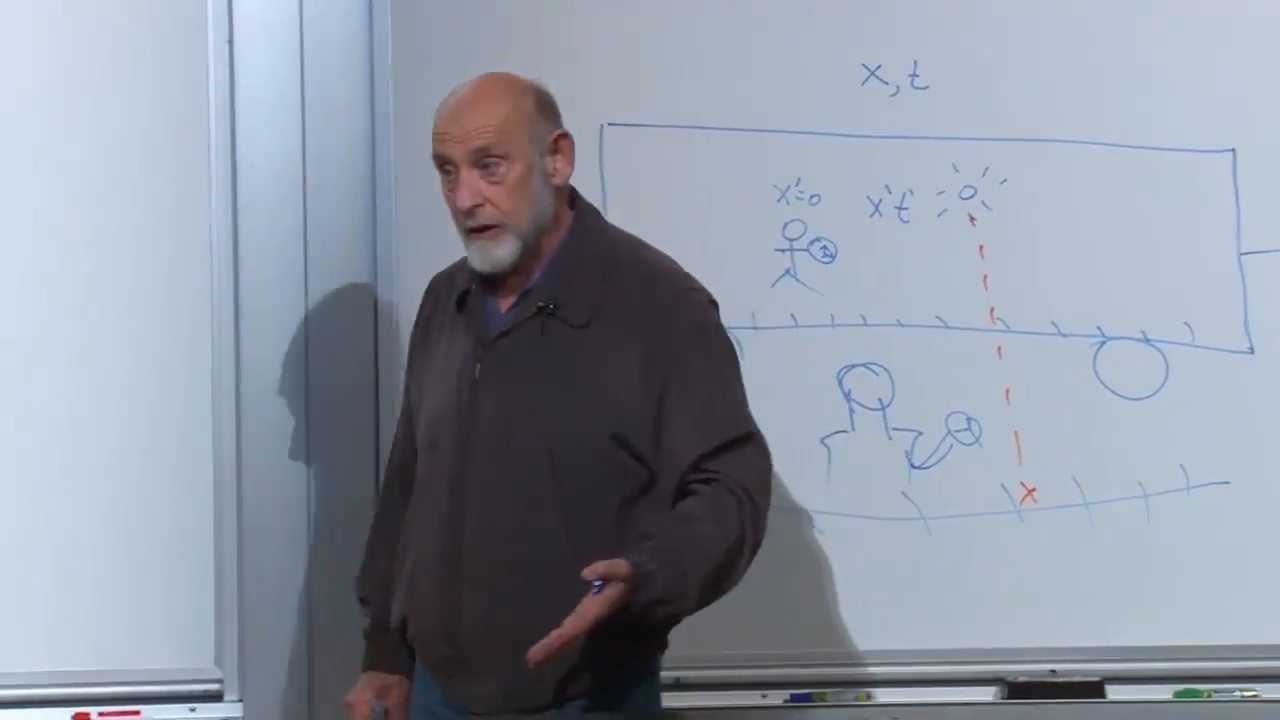
\includegraphics[width=0.90\textwidth]{lecture_02_figure_02.png}
\caption{역변환에도 같은 로렌츠 인자가 나타나며, 상대 속도의 부호만 반대다.}
\lectureframe{00:09:15}
\end{figure}

\(x\)축을 따른 부스트에서는 횡좌표가 변하지 않는다:
\begin{equation}
y'=y,
\qquad
z'=z.
\end{equation}

분모를 살펴보지 않아도 공간 방정식에서 상대 속도를 읽을 수 있다. 열차의 원점은 \(x'=0\)로 정의되므로,
\begin{equation}
x'=0
\quad\Longleftrightarrow\quad
x-vt=0
\quad\Longleftrightarrow\quad
x=vt.
\label{eq:sr2-origin-worldline}
\end{equation}
이 세계선에서 \(t\)의 계수가 역 좌표계로 나타낸 열차의 속도다.

\section{세 기준계와 부스트의 합성}

열차 안에 작은 장난감 자동차를 놓자. 열차는 역에 대해 속력 \(v\)로 움직이고, 자동차는 열차 승객에 대해 통로를 따라 속력 \(u\)로 움직인다. 자동차의 역에 대한 속력을 \(w\)라고 하자. 뉴턴 역학의 직관은 \(w=u+v\)라고 예상하지만, 답은 로렌츠 변환으로 구해야 한다.

이제 좌표계가 세 개다:
\begin{equation}
(x,t),\qquad (x',t'),\qquad (x'',t'').
\end{equation}
첫 번째는 역, 두 번째는 열차, 세 번째는 자동차에 속한다. 열차와 자동차 사이의 변환은 다음과 같다:
\begin{align}
x''&=\gamma_u(x'-ut'),&
t''&=\gamma_u(t'-ux'),
\label{eq:sr2-second-boost}\\
\gamma_u&=\frac{1}{\sqrt{1-u^2}}.
\end{align}

\begin{figure}[htbp]
\centering
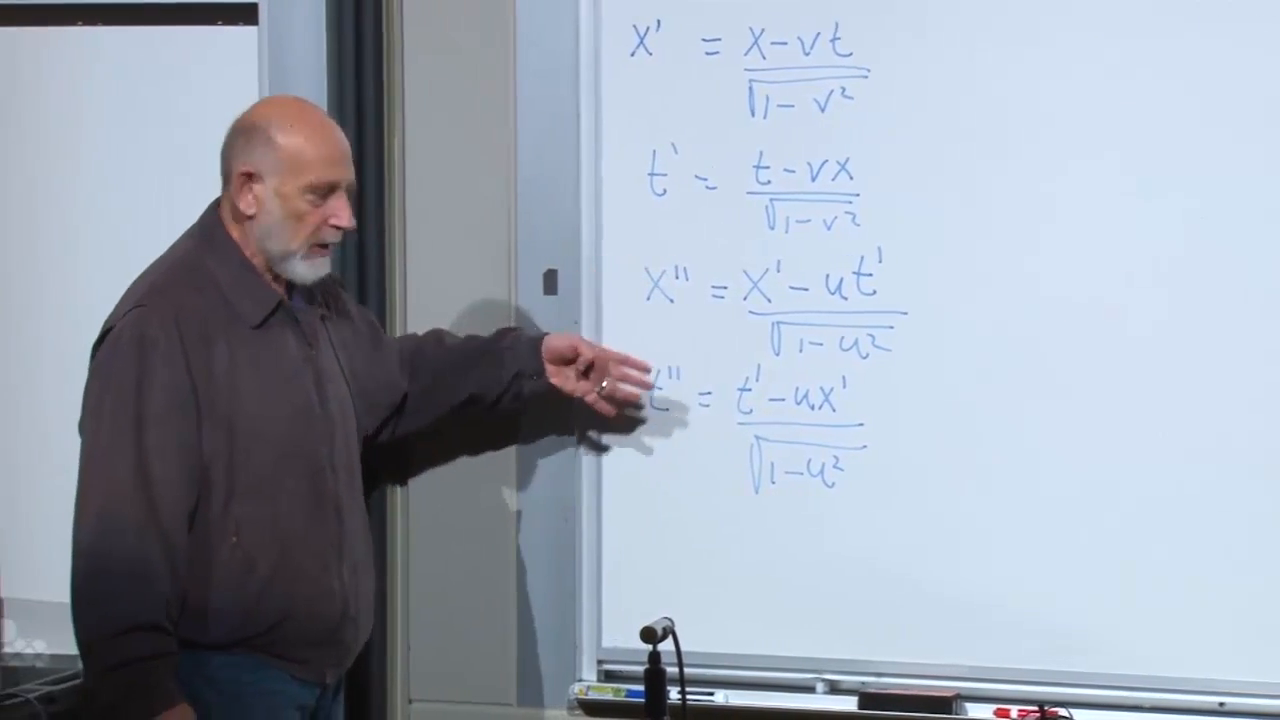
\includegraphics[width=0.90\textwidth]{lecture_02_figure_03.png}
\caption{역에서 프라임 좌표계로 가는 정변환에 이어, 프라임 좌표계에서 이중 프라임 좌표계로 가는 두 번째 로렌츠 변환을 적용한다.}
\lectureframe{00:14:55}
\end{figure}

\subsection{한 부스트를 다른 부스트에 대입하기}

\(w\)를 구하는 데에는 공간 방정식이면 충분하다. \eqref{eq:sr2-direct}를 \eqref{eq:sr2-second-boost}의 첫 번째 방정식에 대입하자:
\begin{align}
x''
&=\gamma_u(x'-ut')\\
&=\gamma_u\gamma_v\left[(x-vt)-u(t-vx)\right]\\
&=\gamma_u\gamma_v\left[(1+uv)x-(u+v)t\right].
\label{eq:sr2-composed-space}
\end{align}
\(uvx\) 항에 있는 두 음수 부호 때문에 그 항은 양수가 된다. 두 시간 항은 \(-(u+v)t\)로 합쳐진다.

\begin{figure}[htbp]
\centering
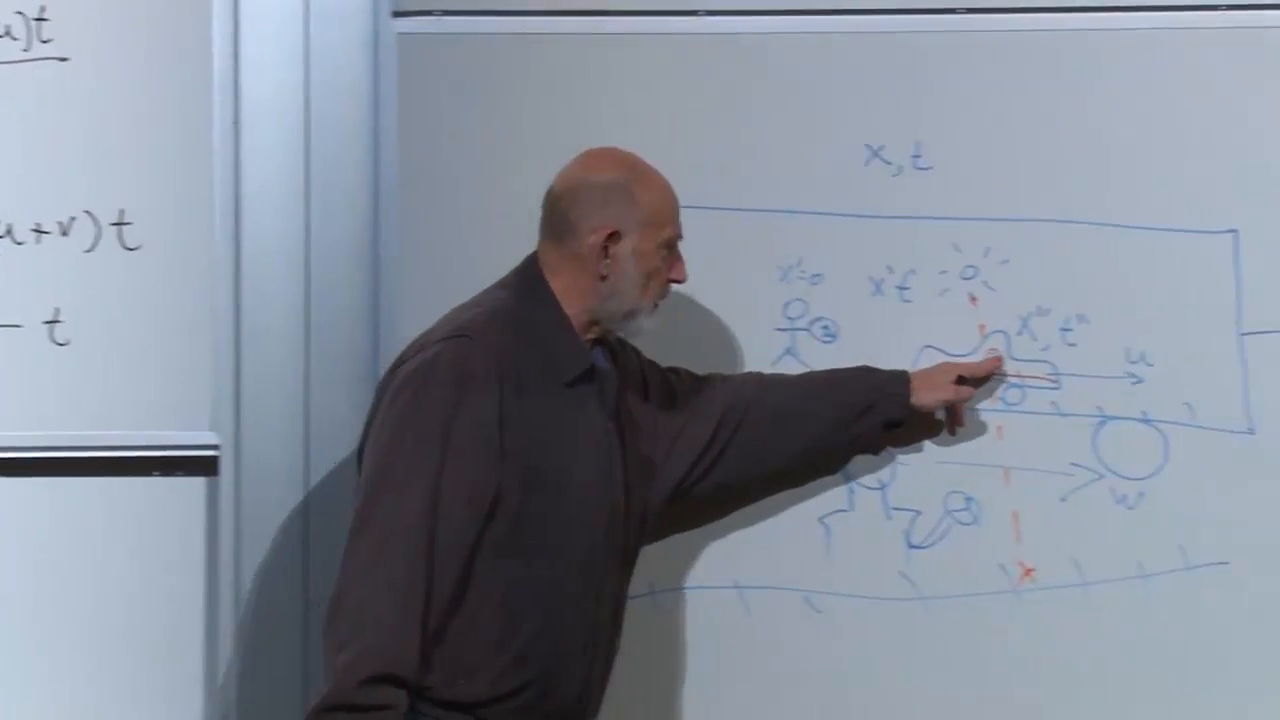
\includegraphics[width=0.91\textwidth]{lecture_02_figure_04.png}
\caption{합성된 부스트에서 \(x\) 항과 \(t\) 항을 모으기 전의 중첩 대입.}
\lectureframe{00:16:30}
\end{figure}

앞서와 마찬가지로, 움직이는 원점의 위치를 찾을 때 분모는 중요하지 않다. 꼬마 자동차는 \(x''=0\)에서 정지해 있으므로, \eqref{eq:sr2-composed-space}의 대괄호 안의 값은 영이어야 한다:
\begin{equation}
(1+uv)x-(u+v)t=0.
\end{equation}
따라서 정거장 좌표계에서 이 자동차의 세계선은
\begin{equation}
x=\frac{u+v}{1+uv}\,t,
\end{equation}
속도는
\begin{equation}
\boxed{w=\frac{u+v}{1+uv}}.
\label{eq:sr2-velocity-add-c1}
\end{equation}

\begin{figure}[htbp]
\centering
\includegraphics[width=0.91\textwidth]{lecture_02_figure_05.png}
\caption{정리한 분자와 세계선 \(x=[(u+v)/(1+uv)]t\)에서 합성된 속도를 알 수 있다.}
\lectureframe{00:19:30}
\end{figure}

시간 방정식도 일관되게 합성된다. 역에서 자동차로 가는 전체 변환은 로렌츠 변환의 형태를 갖는다:
\begin{align}
x''&=\gamma_w(x-wt),&
t''&=\gamma_w(t-wx),
\end{align}
여기서
\begin{equation}
\gamma_w=\frac{1}{\sqrt{1-w^2}}.
\end{equation}
실제로,
\begin{equation}
\gamma_w=\gamma_u\gamma_v(1+uv),
\end{equation}
이는 \eqref{eq:sr2-velocity-add-c1}를 대입하고 식을 정리하면 얻어진다. 따라서 같은 직선상에서 일어나는 두 부스트의 합성은 또 다른 같은 직선상의 부스트다.

\subsection{차원을 복원하기}

\begin{classroomqa}
\audiencequestion{보통 단위에서 분모 \(1+uv\)가 차원상 맞지 않는 이유는 무엇인가?}
\lecturerresponse{이는 \(c=1\)이어서 모든 속도가 빛의 속력에 대한 무차원 비율이 되기 때문에만 맞는 표현이다. 통상적인 단위에서는 곱이 \(uv/c^2\)로 나타나야 하며, 이 양은 무차원이다. \lecturetimestamp{00:21:11}}
\end{classroomqa}

차원을 고려한 속도 합성 법칙은 다음과 같다:
\begin{equation}
\boxed{
w=\frac{u+v}{1+\dfrac{uv}{c^2}}
}.
\label{eq:sr2-velocity-add}
\end{equation}

\begin{figure}[htbp]
\centering
\includegraphics[width=0.90\textwidth]{lecture_02_figure_06.png}
\caption{차원 일관성을 맞추면 곱 \(uv\) 아래에 \(c^2\)이 복원된다.}
\lectureframe{00:22:06}
\end{figure}

\(\lvert u\rvert,\lvert v\rvert\ll c\)일 때,
\begin{equation}
\frac{uv}{c^2}\ll 1,
\end{equation}
따라서
\begin{equation}
w\approx u+v.
\end{equation}
뉴턴식 덧셈은 별개의 법칙이 아니라 저속 근사다.

\subsection{두 가지 수치 영역}

먼저 다음 경우를 보자:
\begin{equation}
u=v=0.01c.
\end{equation}
단위 \(c=1\)에서,
\begin{equation}
w=\frac{0.02}{1.0001}\approx 0.019998.
\end{equation}
빛의 속력의 1퍼센트는 이미 약 \(3\times10^6\ {\rm m/s}\)이지만, 상대론적 보정은 만분의 일에 불과하다. 결과는 뉴턴 역학에서 예상하는 \(0.02c\)보다 약간 작다.

\begin{figure}[htbp]
\centering
\includegraphics[width=0.90\textwidth]{lecture_02_figure_07.png}
\caption{\(u=v=0.01c\)에서 분모는 1과 겨우 \(10^{-4}\)만큼 차이 난다.}
\lectureframe{00:24:23}
\end{figure}

이제 다음 경우를 보자:
\begin{equation}
u=v=0.9c.
\end{equation}
뉴턴 역학에서는 \(1.8c\)를 예측한다. 상대론에서는
\begin{equation}
\frac{w}{c}
=\frac{0.9+0.9}{1+0.9^2}
=\frac{1.8}{1.81}
\approx 0.9945.
\label{eq:sr2-fast-example}
\end{equation}

\begin{figure}[htbp]
\centering
\includegraphics[width=0.90\textwidth]{lecture_02_figure_08.png}
\caption{속력 \(0.9c\)인 두 물체의 속도를 합성하면 \(1.8/1.81\)가 되며, 여전히 빛의 속력보다 작다.}
\lectureframe{00:25:48}
\end{figure}

빛보다 느린 부스트를 연속해서 적용해도 \(c\)를 넘을 수 없다. \(u<c\)이고 \(v<c\)이면,
\begin{equation}
1-\frac{w}{c}
=
\frac{\left(1-\frac{u}{c}\right)
      \left(1-\frac{v}{c}\right)}
     {1+\frac{uv}{c^2}}
>0.
\end{equation}
부스트를 하나씩 더할 때마다 결과는 \(c\)에 더 가까워질 수 있지만, 결코 그 값을 넘지는 않는다. 극한값 \(u=c\)에서는,
\begin{equation}
w=\frac{c+v}{1+v/c}=c.
\end{equation}
빛의 속력은 합성 법칙의 고정점이다.

\section{좌표 측정은 시각적 모습과 다르다}

\begin{classroomqa}
\audiencequestion{열차에 유리 벽이 있다면, 역의 관측자는 승객과 장난감 자동차를 함께 바라보고 그 운동을 직접 알아낼 수 있는가?}
\lecturerresponse{로렌츠 변환은 공간 곳곳에 놓인 막대와 동기화된 시계를 사용해 얻는 좌표 측정에 관한 것이다. 시각적 영상에는 서로 다른 사건에서 관측자에게 도달하는 빛의 이동 시간이 서로 다르다는 점도 반영된다. 유리는 보이는 모습만 바꿀 뿐 좌표 관계는 바꾸지 않는다. 영상 하나를 동시각의 자료로 취급하면 상대론이 바로잡은 동시성 가정을 다시 들여오게 된다. \lecturetimestamp{00:27:53}}
\end{classroomqa}

그 순간에 누군가 사건을 보는지와 관계없이, 각 기준계에서 사건의 위치와 시간은 정해져 있다. 광학적 모습도 정당한 연구 대상이지만, 그러려면 각 사건에서 눈까지 빛이 이동하는 경로를 추적하는 별도의 계산이 필요하다. 변환 법칙 자체는 보편적이며 열차의 벽과 무관하다.

\section{세 공간 차원에서의 고유 간격}

두 사건으로 돌아가자. 첫 번째 사건은 원점에 있고, 두 번째 사건은 \((x,t)\)에 있다고 하자. 공간 차원이 하나일 때는,
\begin{equation}
\tau^2=t^2-x^2
\label{eq:sr2-interval-1d}
\end{equation}
단위 \(c=1\)에서 모든 관성계가 다음 값에 동의한다:
\begin{equation}
\tau^2
=t^2-x^2
=t'^2-x'^2
=t''^2-x''^2.
\end{equation}
좌표는 변하지만 고유 간격은 변하지 않는다.

시간꼴 분리에서는 시계가 두 사건 사이를 이동할 수 있다. 첫 사건에서 정오를 가리키던 시계가 두 번째 사건에서 가리키는 시각까지의 경과 시간은 고유시간 \(\tau\)이다. 어느 좌표계에서 간격을 계산하든 이 진술은 달라지지 않는다.

\begin{figure}[htbp]
\centering
\includegraphics[width=0.90\textwidth]{lecture_02_figure_09.png}
\caption{고유시간의 불변 관계 \(\tau^2=t^2-x^2\)를 상기한 뒤 횡방향을 다시 도입한다.}
\lectureframe{00:30:18}
\end{figure}

\subsection{공간 회전으로 횡방향 복원하기}

부스트를 다시 살펴보기 전에 공간축을 보통 방식으로 회전해 보자. \(x\)축 위에 놓이지 않은 점의 제곱 공간 거리는
\begin{equation}
r^2=x^2+y^2+z^2,
\end{equation}
이며, 보통의 피타고라스 정리에 따라 회전해도 변하지 않는다. 따라서 \(3+1\) 시공간 간격은
\begin{equation}
\boxed{
\tau^2=t^2-x^2-y^2-z^2
}.
\label{eq:sr2-interval-3d}
\end{equation}
\(c\)를 복원하면,
\begin{equation}
c^2\tau^2
=c^2t^2-x^2-y^2-z^2.
\end{equation}

\begin{figure}[htbp]
\centering
\includegraphics[width=0.90\textwidth]{lecture_02_figure_10.png}
\caption{피타고라스 정리에 따른 공간 거리를 이용하면 불변량이 \(t^2-x^2\)에서 \(t^2-x^2-y^2-z^2\)로 확장된다.}
\lectureframe{00:34:23}
\end{figure}

공간 회전과 로렌츠 부스트를 어떻게 조합하든 \eqref{eq:sr2-interval-3d}는 보존된다. 보통의 좌표축들은 성분은 서로 다르게 나타내지만 유클리드 거리는 같게 나타낸다. 관성 시공간 기준계들은 공간과 시간 성분은 서로 다르게 나타내지만 이 제곱들의 차는 같게 나타낸다. 이 불변량이 특수상대성이론의 핵심 기하학적 사실이다.

\begin{classroomqa}
\audiencequestion{승객이 장난감 자동차 대신 앞쪽으로 손전등을 비추면 열차 관측자와 역 관측자는 같은 빛의 속력을 얻는가?}
\lecturerresponse{\(u=c\)를 \eqref{eq:sr2-velocity-add}에 대입하자. 그러면 \(w=(c+v)/(1+v/c)=c\)이다. 단위 \(c=1\)에서는 그 비가 단순히 \((1+v)/(1+v)=1\)이다. 요구되는 대로 두 기준계 모두 정확히 같은 속력을 측정한다. \lecturetimestamp{00:35:53}}
\end{classroomqa}

따라서 앞서 제기된 유리 벽의 문제는 빛의 속력이 불변이라는 사실이 실패하는 경우가 아니다. 좌표 측정과 지연되어 보이는 시각적 영상, 궁극적으로는 동시성에 관한 혼동이다.

\section{빛살과 빛원뿔}

한 공간 차원에서 오른쪽과 왼쪽으로 진행하는 빛살은 다음을 만족한다:
\begin{equation}
x=\pm t.
\end{equation}
이 빛살의 시공간 간격은 영이다:
\begin{equation}
t^2-x^2=0.
\end{equation}
유클리드 거리와 달리, 시공간 간격이 영이라고 해서 두 사건이 일치해야 하는 것은 아니다. 이는 빛 신호가 두 사건을 연결할 수 있음을 뜻한다.

공간 방향을 모두 복원하면 빛살은 다음을 만족한다:
\begin{equation}
t^2-x^2-y^2-z^2=0,
\label{eq:sr2-null}
\end{equation}
또는
\begin{equation}
r=t
\end{equation}
단위 \(c=1\)에서 미래 방향으로 진행하는 빛에 대해 성립한다.

\begin{figure}[htbp]
\centering
\includegraphics[width=0.90\textwidth]{lecture_02_figure_11.png}
\caption{어느 공간 방향으로 진행하든 빛은 \(t^2-(x^2+y^2+z^2)=0\)을 만족하는 영 궤적을 따른다.}
\lectureframe{00:39:28}
\end{figure}

\(1+1\)차원에서는 영집합이 \(45^\circ\)인 두 직선이다. 공간 차원 둘과 시간 차원 하나에서는 원뿔이 된다. 공간 차원이 셋이면 칠판에 온전히 그릴 수 없지만, 이를 정의하는 방정식은 그대로다.

미래 빛원뿔은 원점에서 방출된 빛이 도달할 수 있는 사건들로 이루어진다. 과거 빛원뿔은 빛이 원점에 도달할 수 있는 사건들로 이루어진다. 하나는 다른 하나를 시간에 대해 뒤집은 것이다.

\begin{figure}[htbp]
\centering
\includegraphics[width=0.90\textwidth]{lecture_02_figure_12.png}
\caption{\(45^\circ\)인 영광선들이 더 높은 차원의 시공간 그림에서 미래와 과거 빛원뿔을 이룬다.}
\lectureframe{00:40:47}
\end{figure}

\begin{classroomqa}
\audiencequestion{뉴턴 역학의 갈릴레이 변환에서 이에 대응하는 불변량은 무엇인가?}
\lecturerresponse{시간 간격 자체다. 뉴턴 역학의 관측자들은 공간 변위에는 동의하지 않지만 모두 \(\Delta t\)에는 동의한다. 상대론은 보편적 시간을 포기하고 그 자리에 불변 시공간 간격을 둔다. \lecturetimestamp{00:41:53}}
\end{classroomqa}

\section{공간 벡터에서 사차원 벡터로}

여기서 벡터는 양자 상태 벡터가 아니라 기하학적 벡터다. 보통 공간에서 두 점 사이의 변위에는 크기와 방향이 있다. 벡터의 꼬리를 옮겨 원점에 놓아도 벡터는 바뀌지 않으며, 그 세 성분은 다음과 같이 쓸 수 있다:
\begin{equation}
x^i=(x^1,x^2,x^3)=(x,y,z),
\qquad i=1,2,3.
\end{equation}
라틴 지표 \(i\)는 공간 방향만을 나타낸다.

사건에는 시간이라는 성분이 하나 더 필요하다. 따라서 시공간 위치는 다음과 같이 쓴다:
\begin{equation}
x^\mu=(x^0,x^1,x^2,x^3)=(t,x,y,z),
\qquad \mu=0,1,2,3.
\label{eq:sr2-four-position}
\end{equation}
역사적 관례에 따라 시간은 네 번째 성분이 아니라 영 번째 성분으로 둔다:
\begin{equation}
x^0=t,\qquad x^1=x,\qquad x^2=y,\qquad x^3=z.
\end{equation}
\(\mu\)와 같은 그리스 첨자는 시공간 성분을, \(i\)와 같은 라틴 첨자는 공간 성분을 나타낸다.

\begin{figure}[htbp]
\centering
\includegraphics[width=0.90\textwidth]{lecture_02_figure_13.png}
\caption{공간 성분 \(x^i\)를 네 성분으로 이루어진 시공간 위치 \(x^\mu=(x^0,x^1,x^2,x^3)\)로 확장한다.}
\lectureframe{00:46:05}
\end{figure}

불변량은 다음과 같이 된다:
\begin{equation}
\tau^2
=(x^0)^2-(x^1)^2-(x^2)^2-(x^3)^2.
\end{equation}
이 표기법 자체가 새로운 물리를 더하는 것은 아니다. 그 장점은 로렌츠 변환이 공간 벡터에 회전이 작용하듯 네 성분 모두에 선형으로 작용한다는 데 있다.

\begin{classroomqa}
\audiencequestion{변환이 선형이므로 열벡터에 작용하는 행렬로 나타낼 수 있는가?}
\lecturerresponse{그렇다. \(x\)축 방향 부스트에서는 \(\gamma_v\begin{pmatrix}1&-v\\-v&1\end{pmatrix}\)가 \((t,x)^{\mathsf T}\)에 작용하고, \(y\)와 \(z\)는 변하지 않는다. 로렌츠 변환을 합성하고 정리하는 데 행렬 표기가 자연스럽다. \lecturetimestamp{00:48:14}}
\end{classroomqa}

구체적으로 쓰면,
\begin{equation}
\begin{pmatrix}
t'\\x'\\y'\\z'
\end{pmatrix}
=
\begin{pmatrix}
\gamma_v&-\gamma_v v&0&0\\
-\gamma_v v&\gamma_v&0&0\\
0&0&1&0\\
0&0&0&1
\end{pmatrix}
\begin{pmatrix}
t\\x\\y\\z
\end{pmatrix}.
\label{eq:sr2-boost-matrix}
\end{equation}

\section{변위와 사차원 속도}

한 사건의 위치에서 입자 세계선의 짧은 구간으로 옮겨가 보자. 사차원 변위는 다음과 같다:
\begin{equation}
\Delta x^\mu
=(\Delta t,\Delta x,\Delta y,\Delta z).
\end{equation}
변위가 작다고 할 때 미적분학의 관점으로 다가가며, \(\Delta x^\mu\)는 \(dx^\mu\)가 된다. 지금은 기하를 명확히 보여 주는 유한한 변위 표기를 사용한다.

시간꼴 세계선을 따라 고유시간 증분은 다음을 만족한다:
\begin{equation}
(\Delta\tau)^2
=(\Delta t)^2-(\Delta x)^2-(\Delta y)^2-(\Delta z)^2.
\label{eq:sr2-proper-increment}
\end{equation}
보통의 속도는 공간 변위를 좌표 시간으로 나누며 세 성분을 갖는다. 사차원 속도는 대신 사차원 변위를 불변 고유시간으로 나눈다:
\begin{equation}
u^\mu
=\frac{\Delta x^\mu}{\Delta\tau}
\quad\longrightarrow\quad
\boxed{
u^\mu=\frac{dx^\mu}{d\tau}
}.
\label{eq:sr2-four-velocity}
\end{equation}

\begin{figure}[htbp]
\centering
\includegraphics[width=0.90\textwidth]{lecture_02_figure_14.png}
\caption{세계선의 한 구간은 \(\Delta x^\mu\), 그 불변량 \(\Delta\tau\), 그리고 사차원 속도 \(u^\mu=\Delta x^\mu/\Delta\tau\)를 정의한다.}
\lectureframe{00:52:42}
\end{figure}

이 양은 네 성분을 가지며 사차원 벡터처럼 변환된다. 이것과 보통의 삼차원 속도가 어떻게 관계되는지는 다음 질문이며, 여기서는 일부러 답을 미뤄 둔다. 이 관계를 밝히면 상대론적 운동량, 에너지, 가속도, 그리고 마침내 \(F=ma\)의 상대론적 일반화로 나아가게 된다.
\graphicspath{{../../../generated_course_notes/core/special_relativity/2012_spring_theoretical_minimum/chapters/lecture_03/}{../../../generated_course_notes/core/special_relativity/2012_spring_theoretical_minimum/figures/}{../../../generated_course_notes/core/special_relativity/2012_spring_theoretical_minimum/assets/}}
\chapter{입자 역학, 사차원 운동량, 정지 에너지}

\section{반복해서 사용할 근사}

상대론적 입자의 역학은 익숙한 질문에 새로운 언어로 답해야 합니다. 입자는 어떻게 운동할까요? 운동량과 에너지는 무엇일까요? 이 물리량들은 왜 하나의 사차원 벡터를 이루며, \(E=mc^2\)는 역학의 통상적인 틀에서 어떻게 나올까요? 이 질문들을 다루기 전에, 계산 전반에 걸쳐 반복해서 쓰일 기본적인 근사 하나를 살펴보겠습니다.

임의의 지수 \(p\)에 대해 이항급수는 다음과 같다.
\begin{equation}
\begin{aligned}
(1+\epsilon)^p
&=1+p\epsilon\\
&\quad+\frac{p(p-1)}{2!}\epsilon^2\\
&\quad+\frac{p(p-1)(p-2)}{3!}\epsilon^3
+\cdots .
\end{aligned}
\label{eq:sr3-binomial}
\end{equation}
지수는 양수, 음수, 분수 또는 복소수일 수도 있다. \(\epsilon\)가 충분히 작으면 급수는 빠르게 수렴하고 각 항은 앞 항보다 작아진다. 그러면 원하는 정확도에 필요한 차수에서 급수를 멈출 수 있다. 영차항이 가장 큰 경우가 흔하지만, 아래의 응용에서는 흔히 상수이므로 동역학적으로 중요하지 않다. 운동은 첫 번째 보정항에서 나타난다.

\begin{figure}[htbp]
\centering
\includegraphics[width=0.90\textwidth]{lecture_03_figure_01.png}
\caption{상대론적 공식에서 비상대론적 역학을 도출할 때 사용하는 삼차항까지의 이항급수.}
\lectureframe{00:04:24}
\end{figure}

보통 \(c=1\)로 둡니다. 따라서 속도 \(v\)는 빛의 속도의 \(v/c\)를 뜻합니다. \(\epsilon=-v^2\)로 두고 \(p=\tfrac12\)을 사용하면,
\begin{equation}
\sqrt{1-v^2}
=
1-\frac{v^2}{2}-\frac{v^4}{8}-\cdots
\approx
1-\frac{v^2}{2},
\qquad |v|\ll 1.
\label{eq:sr3-sqrt-expansion}
\end{equation}
\(p=-\tfrac12\)을 사용하면 두 음수 부호가 서로 상쇄됩니다.
\begin{equation}
\frac{1}{\sqrt{1-v^2}}
=
1+\frac{v^2}{2}+\frac{3v^4}{8}+\cdots
\approx
1+\frac{v^2}{2}.
\label{eq:sr3-gamma-expansion}
\end{equation}
고전역학에서 나타나는 많은 \(1/2\) 인자는 사후에 보면 이러한 상대론적 전개 중 하나의 첫 번째 보정항으로 이해할 수 있습니다. \(v\)가 1에 가까워지면 근사는 성립하지 않습니다. 이때는 유한한 차수에서 급수를 끊어도 정확한 식의 특이 거동을 포착할 수 없습니다.

\begin{figure}[htbp]
\centering
\includegraphics[width=0.90\textwidth]{lecture_03_figure_02.png}
\caption{저속에서 두 공식이 모두 드러납니다. \(\sqrt{1-v^2}\approx1-v^2/2\)와 \((1-v^2)^{-1/2}\approx1+v^2/2\)입니다.}
\lectureframe{00:07:39}
\end{figure}

\section{입자란 무엇인가?}

역학에서 입자가 반드시 기본 입자일 필요는 없습니다. 전자일 수도, 태양일 수도, 초콜릿 상자나 도넛일 수도 있습니다. 중요한 것은 물체가 충분히 잘 뭉쳐 있어 전체 운동을 질량중심으로 기술할 수 있다는 점입니다. 도넛은 질량중심이 물질 자체의 내부에 있을 필요는 없다는 사실을 떠올리게 해 줍니다.

뉴턴 역학에서 질량중심 변수는 다음 관계를 따릅니다.
\begin{equation}
\vec p=m\vec v,
\qquad
K=\frac12mv^2,
\qquad
\vec F=m\vec a.
\label{eq:sr3-newtonian-particle}
\end{equation}
이 식들은 물체가 기본 입자인지 복합계인지에 상관하지 않습니다. 복합계에는 내부 에너지도 있습니다. 예를 들어 움직이는 도넛의 에너지는 질량중심의 운동에너지에 화학 에너지, 열에너지, 결합 에너지를 더한 것입니다.
\begin{equation}
E_{\text{Newtonian}}
=
E_{\text{internal}}+\frac12mv^2.
\label{eq:sr3-newtonian-internal}
\end{equation}
내부 항은 전체 질량중심 속도와 무관합니다. 상대론에서도 이 구분은 유지되지만, 내부 에너지가 물체 전체의 불변 질량에 기여한다는 점이 드러납니다.

필요한 도구는 고전역학에서 쓰는 것과 같습니다. 궤적, 정지 작용 원리, 라그랑지안, 정준 운동량, 해밀토니안, 그리고 연속 대칭과 보존 법칙 사이의 관계입니다.

\section{세계선과 인과적 분리}

계의 위치를 가로축에, 시간을 세로축에 그려 보세요. 그러면 계의 이력은 시공간의 곡선이 됩니다. 입자 하나의 경우 이 곡선을 \emph{세계선}이라고 합니다. 이 개념은 뉴턴 역학에도 있지만, 로런츠 변환이 공간과 시간을 섞기 때문에 상대론에서는 근본적인 역할을 합니다.

두 사건 사이의 간격을 다음과 같이 두겠습니다.
\begin{equation}
\Delta x^\mu=(\Delta t,\Delta\vec x),
\qquad
\Delta\vec x^{\,2}
=
(\Delta x)^2+(\Delta y)^2+(\Delta z)^2.
\end{equation}
단위 \(c=1\)에서 두 사건의 불변 간격은 다음과 같습니다.
\begin{equation}
(\Delta\tau)^2
=
(\Delta t)^2-\Delta\vec x^{\,2}.
\label{eq:sr3-interval}
\end{equation}

\subsection{시간꼴 분리}

\((\Delta t)^2>\Delta\vec x^{\,2}\)이면 \((\Delta\tau)^2>0\)이고, 두 사건은 시간꼴로 분리되어 있습니다. 두 사건이 같은 공간 위치에서 일어나는 로런츠 기준계가 존재합니다. 그 기준계에서는 두 사건을 잇는 선이 수직이며, 시계가 한 사건에서 다른 사건으로 이동할 수 있습니다. 그 시계가 기록한 경과 시간이 고유 시간 \(\Delta\tau\)입니다.

\begin{figure}[htbp]
\centering
\includegraphics[width=0.90\textwidth]{lecture_03_figure_03.png}
\caption{시간꼴 간격에서는 시간 방향의 분리가 공간 방향의 분리보다 크며, 두 사건이 같은 위치에 있는 정지 기준계가 존재합니다.}
\lectureframe{00:14:42}
\end{figure}

\subsection{공간꼴 분리}

\(\Delta\vec x^{\,2}>(\Delta t)^2\)이면 간격은 공간꼴입니다. 두 사건이 같은 공간 위치에서 일어나는 관성계는 없지만, 두 사건이 동시에 일어나는 기준계는 있습니다. 다른 기준계에서는 시간 순서가 뒤바뀔 수도 있습니다. 따라서 공간꼴로 분리된 사건 쌍에 대해 \emph{사건 \(A\)이 먼저 일어났다}거나 \emph{사건 \(B\)이 먼저 일어났다}고 하는 것은 불변인 진술이 아닙니다. 이것이 기하학적 형태로 표현한 동시성의 상대성입니다.

\begin{figure}[htbp]
\centering
\includegraphics[width=0.90\textwidth]{lecture_03_figure_04.png}
\caption{공간꼴 간격에서는 관성계를 바꾸면 두 사건이 동시에 일어나게 하거나 시간 순서를 뒤바꿀 수 있습니다.}
\lectureframe{00:17:01}
\end{figure}

질량을 가진 입자의 세계선은 시간꼴입니다. 충분히 짧은 모든 구간에서 \(d\tau^2>0\)를 만족합니다. \(0.9c\)인 속도를 차례로 합성하면 입자를 \(c\)에 점점 더 가깝게 만들 수는 있지만, 그보다 빠르게 할 수는 없습니다. 이는 제논의 역설과 비슷한 점이 있습니다. 이러한 인과적 제약은 물질적 물체뿐 아니라 신호와 정보에도 적용됩니다. 정보도 물리적 계를 통해 전달되어야 하기 때문입니다. 빛보다 빠른 신호가 있다면 기준계에 따라 그 신호의 이력에서 어느 쪽이 원인이고 어느 쪽이 결과인지 의견이 달라질 수 있습니다.

\section{사차원 속도}

시간꼴인 짧은 구간을 살펴봅시다. 통상적인 단위로 쓰면,
\begin{equation}
d\tau
=
\sqrt{dt^2-\frac{d\vec x^{\,2}}{c^2}}.
\label{eq:sr3-proper-time-dimensional}
\end{equation}
\(c^2\) 인자는 차원 일치 조건에 따라 정해집니다. \(dt^2\)의 단위는 시간의 제곱인 반면, \(d\vec x^{\,2}\)의 단위는 길이의 제곱입니다.

\begin{classroomqa}
\audiencequestion{간격을 통상적인 단위로 쓸 때 빛의 속도는 어디에 넣어야 할까요?}
\lecturerresponse{공간 항을 \(c^2\)로 나누어야 하므로 \(d\tau^2=dt^2-d\vec x^{\,2}/c^2\)가 됩니다. 보통은 다시 \(c=1\)로 두겠지만, 차원 일치 조건을 따르면 빠진 인자를 언제든 복원할 수 있습니다. \lecturetimestamp{00:21:23}}
\end{classroomqa}

\begin{figure}[htbp]
\centering
\includegraphics[width=0.90\textwidth]{lecture_03_figure_05.png}
\caption{세계선의 변위 \(\Delta x^\mu=(\Delta t,\Delta\vec x)\)와 그에 대응하는 고유 시간의 증가량.}
\lectureframe{00:21:03}
\end{figure}

통상적인 속도는 세 개의 공간 성분을 가집니다.
\begin{equation}
v^i=\frac{dx^i}{dt},
\qquad i=1,2,3.
\end{equation}
상대론적 속도는 시공간 변위 전체를 불변인 고유 시간으로 나누어 얻습니다.
\begin{equation}
u^\mu
=
\frac{dx^\mu}{d\tau},
\qquad
\mu=0,1,2,3.
\label{eq:sr3-four-velocity-definition}
\end{equation}
그리스 문자 첨자는 시공간 성분을, 라틴 문자 첨자는 공간 성분을 가리킵니다. \(x^0=t\)이며 단위가 \(c=1\)이므로,
\begin{equation}
u^0=\frac{dt}{d\tau}.
\end{equation}

\begin{figure}[htbp]
\centering
\includegraphics[width=0.90\textwidth]{lecture_03_figure_06.png}
\caption{통상적인 속도는 공간 변위를 좌표 시간으로 나누지만, 사차원 속도는 네 성분 모두를 고유 시간으로 나눕니다.}
\lectureframe{00:24:05}
\end{figure}

\(u^\mu\)와 \(\vec v\)의 관계를 구하기 위해 간격 식에서 \(dt^2\)를 묶어 내면,
\begin{align}
d\tau^2
&=dt^2-d\vec x^{\,2}\\
&=dt^2\left(1-\frac{d\vec x^{\,2}}{dt^2}\right)
=dt^2(1-v^2).
\end{align}
미래 방향을 향하는 세계선이므로 양의 제곱근을 취하면,
\begin{equation}
\frac{d\tau}{dt}=\sqrt{1-v^2},
\qquad
\frac{dt}{d\tau}=\frac{1}{\sqrt{1-v^2}}
\equiv\gamma.
\label{eq:sr3-time-component}
\end{equation}
공간 성분에 대해서는,
\begin{equation}
v^i
=
\frac{dx^i}{dt}
=
\frac{dx^i}{d\tau}\frac{d\tau}{dt}
=u^i\sqrt{1-v^2}.
\end{equation}
따라서,
\begin{equation}
\boxed{
u^\mu
=
\gamma(1,\vec v)
},
\qquad
u^0=\gamma,
\qquad
u^i=\gamma v^i.
\label{eq:sr3-four-velocity-components}
\end{equation}
저속에서는 \(u^0\to1\)이고 \(u^i\to v^i\)입니다. 빛의 속도에 가까워지면 \(u^0\)와 공간 사차원 속도의 크기는 모두 커지지만, \(|\vec v|<1\)입니다.

\begin{figure}[htbp]
\centering
\includegraphics[width=0.90\textwidth]{lecture_03_figure_07.png}
\caption{통상적인 속도와 \(u^\mu\)의 네 성분 사이의 관계를 정리한 식.}
\lectureframe{00:30:40}
\end{figure}

\subsection{독립 성분은 왜 세 개뿐인가}

사차원 속도는 성분이 네 개지만 독립 자유도는 세 개뿐입니다. 간격 항등식을 \(d\tau^2\)로 나누면,
\begin{equation}
1
=
\left(\frac{dt}{d\tau}\right)^2
-\left(\frac{d\vec x}{d\tau}\right)^2,
\end{equation}
또는
\begin{equation}
\boxed{
(u^0)^2-\vec u^{\,2}=1
}.
\label{eq:sr3-four-velocity-normalization}
\end{equation}
이 하나의 정규화 조건이 독립 성분 하나를 없앱니다.

\begin{figure}[htbp]
\centering
\includegraphics[width=0.90\textwidth]{lecture_03_figure_08.png}
\caption{불변 간격에서 정규화 조건 \((u^0)^2-\vec u^{\,2}=1\)가 바로 얻어집니다.}
\lectureframe{00:33:50}
\end{figure}

\begin{classroomqa}
\audiencequestion{고유 시간 자체에 대해 미분하면 독립 성분 하나가 줄어드는 이유를 이해할 수 있나요?}
\lecturerresponse{그렇습니다. 고유 시간은 독립적인 다섯 번째 좌표가 아닙니다. 고유 시간은 세계선을 따라 시공간 간격으로 정해집니다. 이 정의 관계를 \(d\tau^2\)로 나누면 네 미분 성분은 단위 시간꼴 쌍곡면 \((u^0)^2-\vec u^{\,2}=1\) 위에 놓인다는 제약을 받습니다. \lecturetimestamp{00:34:07}}
\end{classroomqa}

\section{자유 입자의 불변 작용}

힘이 작용하지 않는 세계선은 어떤 법칙을 따를까요? 고전역학에서 두 가지 교훈을 이어받습니다.
\begin{enumerate}
\item 양 끝점을 고정했을 때 물리적 경로는 작용을 정상값으로 만듭니다.
\item 작용은 경로를 이루는 무한소 구간들의 합으로 구성됩니다.
\end{enumerate}
상대론은 세 번째 조건을 더합니다. 모든 관성 관측자가 작용에 동의해야 합니다. 시간꼴 세계선에서 자연스럽게 사용할 수 있는 무한소 스칼라는 \(d\tau\)입니다. 그러므로 자유 입자의 작용은 다음과 같습니다.
\begin{equation}
\boxed{
S=-m\int_a^b d\tau
}
\qquad(c=1).
\label{eq:sr3-invariant-action}
\end{equation}
유한합으로 나타내면,
\begin{equation}
S=-m\lim_{N\to\infty}\sum_{k=1}^{N}\Delta\tau_k.
\end{equation}
모든 관측자가 각 고유 시간 증가량에 동의하므로, 합이 정상값을 갖게 하는 경로에도 모두 동의합니다.

\begin{figure}[htbp]
\centering
\includegraphics[width=0.90\textwidth]{lecture_03_figure_09.png}
\caption{고정된 양 끝점 사이에서 변분하는 세계선을 따라 불변인 고유 시간 증가량을 더해 작용을 구성합니다.}
\lectureframe{00:38:30}
\end{figure}

\begin{classroomqa}
\audiencequestion{작용에 임의의 상수를 곱하면 에너지는 어떻게 되는가?}
\lecturerresponse{에너지는 출발점이 되는 불변량이 아니라 라그랑지안과 해밀토니안으로부터 유도된다. 작용 전체에 영이 아닌 상수를 곱해도 정지 경로는 바뀌지 않지만, 그 작용으로부터 정의되는 정준량의 크기는 달라진다. 유도된 물리량이 확립된 뉴턴 역학의 관례와 일치하도록 정규화 \(-m\)를 선택한다. \lecturetimestamp{00:39:47}}
\end{classroomqa}

\begin{classroomqa}
\audiencequestion{고유 시간 같은 불변량은 작용을 구성하는 출발점으로 왜 적절한가요?}
\lecturerresponse{정지 작용 법칙은 모든 관성계에서 같은 물리적 경로를 골라야 하기 때문입니다. 이는 유클리드 평면에서 최단 곡선을 찾는 것과 비슷합니다. 회전하면 좌표 성분은 바뀌지만 각 무한소 길이는 바뀌지 않으므로, 최단 곡선이 무엇인지도 달라질 수 없습니다. 유클리드 길이를 고유 시간으로 바꾸면 상대론적 구성이 됩니다. \lecturetimestamp{00:40:39}}
\end{classroomqa}

\begin{classroomqa}
\audiencequestion{고유 시간에는 왜 음의 제곱근이 아니라 양의 제곱근을 선택하나요?}
\lecturerresponse{고유 시간은 과거에서 미래로 이동하는 시계가 기록한 양의 경과 시간으로 정의됩니다. 일관되게 음의 제곱근을 택하면 작용의 부호만 뒤집혀 극댓값이 극솟값으로 바뀔 뿐, 정상 세계선은 바뀌지 않습니다. 시계의 정지 기준계에서는 양의 부호를 택했을 때 \(d\tau=dt\)입니다. \lecturetimestamp{00:42:59}}
\end{classroomqa}

인자 \(-m\) 역시 뉴턴 역학을 되찾기 위해 선택한 정규화 관례입니다. 단위를 복원하면 통상적인 작용은 다음과 같습니다.
\begin{equation}
S=-mc^2\int_a^b d\tau.
\label{eq:sr3-action-dimensional}
\end{equation}

\begin{figure}[htbp]
\centering
\includegraphics[width=0.90\textwidth]{lecture_03_figure_10.png}
\caption{유한한 고유 시간 합은 자연 단위계에서 불변 적분 \(-m\int d\tau\)이 됩니다.}
\lectureframe{00:46:23}
\end{figure}

\section{상대론적 라그랑지안}

작용을 표준적인 역학 형태로 나타내기 위해 \(d\tau\)에서 \(dt\)를 묶어 내면,
\begin{equation}
d\tau
=dt\sqrt{1-\dot{\vec x}^{\,2}},
\qquad
\dot{\vec x}^{\,2}
=\dot x^2+\dot y^2+\dot z^2.
\end{equation}
그러면,
\begin{equation}
S
=
\int_a^b L\,dt,
\qquad
\boxed{
L=-m\sqrt{1-v^2}
}
\quad(c=1).
\label{eq:sr3-relativistic-lagrangian}
\end{equation}
통상적인 단위로는,
\begin{equation}
L=-mc^2\sqrt{1-\frac{v^2}{c^2}}.
\label{eq:sr3-relativistic-lagrangian-c}
\end{equation}
이것이 자유 입자의 라그랑지안입니다. 속도에는 의존하지만 위치에는 의존하지 않습니다. 아직 힘이나 퍼텐셜은 도입하지 않았습니다.

\begin{figure}[htbp]
\centering
\includegraphics[width=0.90\textwidth]{lecture_03_figure_11.png}
\caption{\(dt\)를 묶어 내면 세 속도 성분의 함수인 자유 상대론적 라그랑지안이 드러납니다.}
\lectureframe{00:49:57}
\end{figure}

\subsection{라그랑주 역학과 뉴턴 역학의 복원}

\eqref{eq:sr3-sqrt-expansion}을 대입하면,
\begin{align}
L
&=-m\sqrt{1-v^2}\\
&\approx-m\left(1-\frac{v^2}{2}\right)\\
&=-m+\frac12mv^2.
\label{eq:sr3-lagrangian-low-speed}
\end{align}
상수 \(-m\)는 위치와 속도 모두에 무관합니다. 양 끝의 시간이 같은 모든 경로에 동일한 값을 더하므로 오일러--라그랑주 방정식에서는 사라집니다. 동역학적 내용을 담는 부분은 바로 다음 식입니다.
\begin{equation}
L_{\mathrm{Newton}}=\frac12mv^2.
\end{equation}
따라서 불변 작용의 부호와 질량 정규화는 올바르게 선택되었습니다.

\begin{figure}[htbp]
\centering
\includegraphics[width=0.90\textwidth]{lecture_03_figure_12.png}
\caption{저속 전개에는 상수 \(-m\)와 뉴턴 역학의 자유 입자 라그랑지안 \(mv^2/2\)가 남습니다.}
\lectureframe{00:53:24}
\end{figure}

지금 다루는 자유 입자의 경우 오일러--라그랑주 방정식은 속도가 일정하고 시공간 세계선이 직선임을 말해 줄 뿐입니다. 더 중요한 과제는 보존되는 운동량과 에너지를 찾아내는 것입니다.

\section{정준 운동량}

\(L\)에는 위치 의존성이 없으므로 공간 병진에 대해 불변입니다. 이에 대응하는 보존량은 운동량입니다. 뉴턴 역학의 공식 \(p_i=mv_i\)를 가정하지 않고, 정준 정의를 사용합니다.
\begin{equation}
p_i=\frac{\partial L}{\partial\dot x^i}.
\label{eq:sr3-canonical-momentum}
\end{equation}
\(L=-m\sqrt{1-v^2}\)에 대해,
\begin{align}
p_i
&=
-m\frac{1}{2\sqrt{1-v^2}}
\frac{\partial}{\partial\dot x^i}(1-v^2)\\
&=
-m\frac{1}{2\sqrt{1-v^2}}(-2\dot x^i)\\
&=
\frac{mv_i}{\sqrt{1-v^2}}
=m\gamma v_i.
\label{eq:sr3-relativistic-momentum}
\end{align}
\(u^i=\gamma v^i\)이므로,
\begin{equation}
\boxed{
p^i=mu^i
}.
\label{eq:sr3-momentum-spatial}
\end{equation}
저속에서는 \(p^i\approx mv^i\)로 환원됩니다. 빛의 속도에 가까워지면 분모가 결정적으로 중요해집니다.

\begin{figure}[htbp]
\centering
\includegraphics[width=0.90\textwidth]{lecture_03_figure_13.png}
\caption{제곱근 라그랑지안을 정준 방식으로 미분하면 \(p_x=mv_x/\sqrt{1-v^2}\)를 얻습니다.}
\lectureframe{00:58:49}
\end{figure}

\subsection{상대론적 질량이 아닌 질량}

여기서 \(m\)는 단순히 입자의 질량입니다. 입자가 움직여도 변하지 않는 불변 표지입니다. 오래된 교재에서는 이를 \emph{정지 질량}이라 하고, \(E/c^2\)를 속도에 따라 달라지는 \emph{상대론적 질량}이라 부르기도 합니다. 현대적 용법에서는 이러한 구분을 피합니다. 운동에 따라 변하는 것은 에너지와 운동량이지 불변 질량이 아닙니다. 전자의 질량을 나타내는 매개변수는 모든 기준계에서 같습니다.

\section{삼차원 운동량에서 사차원 운동량으로}

사차원 벡터의 한 성분에 관한 진술은 일반적으로 기준계에 따라 달라진다. 예를 들어 \(\Delta\vec x=0\)는 한 기준계에서 두 사건의 위치가 같음을 뜻하지만, 부스트를 가하면 그 간격의 방향이 기울어져 \(\Delta\vec x'\ne0\)가 된다. 반면,
\begin{equation}
\Delta x^\mu=0
\end{equation}
은 불변이다. 한 기준계에서 네 성분이 모두 영이면 모든 기준계에서 네 성분이 모두 영이다. 마찬가지로 \(\vec u=0\)는 입자의 정지계만 특정할 뿐, 사차원 속도에 대한 불변적인 설명은 아니다.

고립계의 통상적인 운동량 보존 법칙은 다음과 같습니다.
\begin{equation}
\vec P_{\mathrm{initial}}-\vec P_{\mathrm{final}}=0.
\label{eq:sr3-three-momentum-conservation}
\end{equation}
이는 삼차원 벡터 방정식입니다. 보존을 로런츠 공변적으로 명시하려면 세 \(p^i=mu^i\)와 함께 들어갈 네 번째 성분이 필요합니다. 자연스러운 완성은 다음과 같습니다.
\begin{equation}
p^\mu=mu^\mu.
\label{eq:sr3-four-momentum}
\end{equation}
\(c=1\) 단위에서는,
\begin{equation}
p^\mu=(p^0,\vec p)
=
m\gamma(1,\vec v).
\end{equation}

\begin{figure}[htbp]
\centering
\includegraphics[width=0.90\textwidth]{lecture_03_figure_14.png}
\caption{공간 성분에 네 번째 성분을 더해야 운동량 보존을 불변인 형태로 나타낼 수 있습니다.}
\lectureframe{01:09:51}
\end{figure}

빠진 성분도 보존되어야 합니다. 입자 역학에는 이미 다른 보존량이 있습니다. 바로 에너지입니다. \(p^0=mu^0=m\gamma\)가 자연 단위계에서 에너지와 정확히 같은지 묻는 문제에는 해밀토니안을 통해 체계적으로 답할 수 있습니다.

\section{해밀토니안은 에너지다}

이 형태의 시간 독립 라그랑지안에서 해밀토니안은 다음과 같습니다.
\begin{equation}
H=\sum_{i=1}^{3}\dot x^i p_i-L.
\label{eq:sr3-hamiltonian-definition}
\end{equation}
이 공식은 뉴턴 역학에만 해당하는 것이 아닙니다. 이는 속도에서 정준 운동량으로 가는 일반적인 르장드르 변환이며, 상대론적 라그랑지안에도 똑같이 적용됩니다.

\begin{figure}[htbp]
\centering
\includegraphics[width=0.90\textwidth]{lecture_03_figure_15.png}
\caption{일반적인 해밀토니안 공식 \(H=\sum_i\dot x^i p_i-L\).}
\lectureframe{01:11:55}
\end{figure}

\(p_i=m\dot x_i/\sqrt{1-v^2}\)와 \(L=-m\sqrt{1-v^2}\)를 대입하면,
\begin{align}
H
&=
\frac{mv^2}{\sqrt{1-v^2}}
+m\sqrt{1-v^2}\\
&=
\frac{mv^2+m(1-v^2)}{\sqrt{1-v^2}}\\
&=
\boxed{\frac{m}{\sqrt{1-v^2}}}
=m\gamma.
\label{eq:sr3-hamiltonian-result}
\end{align}
상쇄가 핵심 단계입니다. \(u^0=\gamma\)와 비교하면,
\begin{equation}
H=mu^0=p^0.
\end{equation}
따라서 네 번째 성분은 에너지입니다.
\begin{equation}
p^\mu=(E,\vec p),
\qquad
E=H
\qquad(c=1).
\label{eq:sr3-four-momentum-natural}
\end{equation}

\begin{figure}[htbp]
\centering
\includegraphics[width=0.90\textwidth]{lecture_03_figure_16.png}
\caption{해밀토니안의 두 항을 공통 분모로 통분하면 \(mv^2\) 항들이 상쇄됩니다.}
\lectureframe{01:14:28}
\end{figure}

\begin{classroomqa}
\audiencequestion{공식 \(H=\sum_i\dot x^i p_i-L\)는 고전 해밀토니안 공식에만 해당하나요?}
\lecturerresponse{이는 특별한 비상대론적 가정이 아니라 라그랑지안에 대응하는 일반적인 르장드르 변환입니다. 어떤 역학이 나오는지는 \(L\)의 형태가 결정합니다. 여기서는 상대론적 제곱근 라그랑지안으로부터 \(H=m/\sqrt{1-v^2}\)를 얻습니다. \lecturetimestamp{01:15:21}}
\end{classroomqa}

이제 불변인 보존 법칙은 다음과 같습니다.
\begin{equation}
\sum_{\mathrm{initial}}p^\mu
=
\sum_{\mathrm{final}}p^\mu,
\label{eq:sr3-four-momentum-conservation}
\end{equation}
이 하나의 사차원 벡터 방정식에 에너지와 운동량의 세 성분 보존이 모두 들어 있습니다.

\section{정지 에너지와 뉴턴 극한}

자연 단위계에서 정확한 에너지는 다음과 같습니다.
\begin{equation}
E=\frac{m}{\sqrt{1-v^2}}.
\end{equation}
\eqref{eq:sr3-gamma-expansion}을 사용하면,
\begin{equation}
E
\approx
m+\frac12mv^2+\frac38mv^4+\cdots .
\label{eq:sr3-energy-natural-expansion}
\end{equation}
두 번째 항은 익숙한 운동에너지입니다. 첫 번째 항은 질량중심이 정지해 있을 때도 남는 에너지입니다.

\begin{figure}[htbp]
\centering
\includegraphics[width=0.90\textwidth]{lecture_03_figure_17.png}
\caption{단위 \(c=1\)에서 정확한 에너지를 전개하면 \(m+mv^2/2+\cdots\)이 됩니다.}
\lectureframe{01:18:02}
\end{figure}

정확한 식에서 차원을 복원해 봅시다. 제곱근 안의 비는 \(v^2/c^2\)이어야 하고, 분자는 에너지 단위를 가져야 합니다.
\begin{equation}
\boxed{
E
=
\gamma mc^2
=
\frac{mc^2}{\sqrt{1-v^2/c^2}}
}.
\label{eq:sr3-energy-exact}
\end{equation}
저속 전개는 다음과 같습니다.
\begin{equation}
\boxed{
E
=
mc^2+\frac12mv^2
+\frac38m\frac{v^4}{c^2}
+\cdots
}.
\label{eq:sr3-energy-dimensional-expansion}
\end{equation}
정지 상태에서는,
\begin{equation}
\boxed{E_{\mathrm{rest}}=mc^2}.
\label{eq:sr3-emc2}
\end{equation}

\begin{figure}[htbp]
\centering
\includegraphics[width=0.90\textwidth]{lecture_03_figure_18.png}
\caption{차원을 복원하면 상수항은 \(mc^2\)가 되고, 그 다음에 뉴턴 역학의 운동에너지 \(mv^2/2\)가 이어집니다.}
\lectureframe{01:19:16}
\end{figure}

이는 기본 입자뿐 아니라 모든 고립된 물체에 적용됩니다. \emph{정지 상태}란 질량중심이 정지해 있다는 뜻입니다. 물체 내부의 분자, 원자, 장은 여전히 움직이고 상호작용할 수 있습니다. 이들의 내부 운동에너지, 퍼텐셜 에너지, 결합 에너지는 모두 총 정지 에너지에 기여하며, 따라서 물체의 불변 질량에도 기여합니다.

\begin{classroomqa}
\audiencequestion{변환 계수가 \(c^2\)를 임의의 수로 나눈 값일 수도 있나요?}
\lecturerresponse{차원만으로는 \(c\)의 거듭제곱만 정해지지만, 계수는 자연 단위계의 결과로 결정됩니다. 통상적인 단위의 공식은 \(c=1\)일 때 \(E=m\)로 환원되어야 합니다. 따라서 차원을 복원한 식은 정지 상태에서 계수가 1인 \(E=mc^2\)입니다. \lecturetimestamp{01:22:08}}
\end{classroomqa}

\begin{classroomqa}
\audiencequestion{이항 전개의 첫 번째 1은 물리적으로 중요하며, 고차항은 무엇을 뜻하나요?}
\lecturerresponse{그렇습니다. 에너지 전개에서 맨 앞의 항은 정지 에너지 \(mc^2\)가 됩니다. 다음 항은 뉴턴 역학의 운동에너지이고, 그보다 높은 차수의 항은 모두 상대론적 보정항입니다. 야구공에서는 무시할 수 있지만 \(v\)가 \(c\)에 가까워지면 반드시 고려해야 합니다. \lecturetimestamp{01:22:37}}
\end{classroomqa}

\(v\to c\)일 때 정확한 에너지와 운동량은 발산합니다.
\begin{equation}
\begin{aligned}
E&=\gamma mc^2\longrightarrow\infty,\\
\vec p&=\gamma m\vec v\longrightarrow\infty
\qquad(m>0).
\end{aligned}
\end{equation}
그러므로 빛의 속도에 도달하려면 에너지와 운동량이 무한대여야 합니다. 유한한 시간 동안 작용하는 유한한 힘은 유한한 충격량만 전달하므로, 질량을 가진 입자는 \(c\)에 가까워질 수는 있어도 도달할 수는 없습니다.

\begin{classroomqa}
\audiencequestion{이제 무엇이 빛의 속도 장벽을 강제하나요?}
\lecturerresponse{정확한 사차원 운동량이 그렇게 합니다. 질량을 가진 입자가 \(c\)에 가까워지면 에너지와 운동량이 모두 발산하는 한편, 사차원 운동량 보존은 모든 상호작용을 제약합니다. 앞서 사차원 속도를 정규화한 것도 운동학적 형태로는 같은 내용을 말합니다. \lecturetimestamp{01:24:27}}
\end{classroomqa}

\section{복합계의 질량}

두 입자가 크기는 같고 방향은 반대인 운동량을 가지고 움직인다고 하자. 두 입자의 총 삼차원 운동량은 영이므로, 우리는 이미 결합계의 정지계에 있다. 이 계의 불변 질량 \(M\)는 이 기준계에서의 총에너지로 정의된다.
\begin{equation}
Mc^2=E_{\mathrm{tot}}
\qquad
(\vec P_{\mathrm{tot}}=0).
\end{equation}
보다 일반적으로는,
\begin{equation}
M^2c^4
=
E_{\mathrm{tot}}^2-c^2\vec P_{\mathrm{tot}}^{\,2}.
\label{eq:sr3-composite-mass}
\end{equation}

\begin{classroomqa}
\audiencequestion{서로 반대 방향으로 움직이는 두 입자를 합친 계의 질량은 각 입자 질량의 합보다 큰가?}
\lecturerresponse{두 입자가 자유 입자라면 그렇다. 질량중심계에서는 두 입자의 운동에너지가 총 정지에너지에 더해지므로 \(M>m_1+m_2\)가 된다. 인력에 의한 결합에너지는 반대로 총에너지를 낮출 수 있으며, 이때는 \(M<m_1+m_2\)가 된다. 불변 질량은 총 운동량이 영인 기준계에서의 총에너지로 정의된다. \lecturetimestamp{01:25:06}}
\end{classroomqa}

복합 물체의 질량을 잴 때 내부 운동과 결합을 무시할 수 없는 이유가 여기에 있습니다. 불변 질량은 구성 입자들의 질량을 단순히 산술적으로 더한 값이 아니라, 고립계 전체에 속합니다.

\begin{classroomqa}
\audiencequestion{정지 에너지 항은 양자 상태의 위상에서 어떤 역할을 하나요?}
\lecturerresponse{에너지가 정해진 상태는 시간에 따라 위상 \(\exp(-iEt/\hbar)\)로 진화하므로, 정지한 입자는 \(\exp(-imc^2t/\hbar)\)를 기여합니다. 공통적인 전체 위상은 관측할 수 없지만, 에너지가 다른 성분들 사이의 상대 위상은 관측할 수 있습니다. 이러한 양자적 결과는 여기서의 고전적 유도와 양립하지만, 그 유도에 필요한 것은 아닙니다. \lecturetimestamp{01:26:57}}
\end{classroomqa}

\section{에너지--운동량 관계}

사차원 속도의 정규화 조건에서 사차원 운동량의 불변 노름이 바로 나옵니다. \(c=1\) 단위계에서는,
\begin{equation}
(u^0)^2-\vec u^{\,2}=1.
\end{equation}

\(m^2\)를 곱하고 \(p^\mu=mu^\mu\)를 사용하면,
\begin{equation}
\boxed{
E^2-\vec p^{\,2}=m^2
}
\qquad(c=1).
\label{eq:sr3-mass-shell-natural}
\end{equation}
같은 식을 다음과 같이 쓸 수도 있습니다.
\begin{equation}
E=\sqrt{\vec p^{\,2}+m^2}.
\end{equation}

\begin{figure}[htbp]
\centering
\includegraphics[width=0.90\textwidth]{lecture_03_figure_19.png}
\caption{사차원 속도 정규화 식에 \(m^2\)를 곱하면 \(E^2-\vec p^{\,2}=m^2\)를 얻습니다.}
\lectureframe{01:31:48}
\end{figure}

\(c\)를 복원하면,
\begin{equation}
\boxed{
E^2
=
\vec p^{\,2}c^2+m^2c^4
},
\qquad
E=\sqrt{\vec p^{\,2}c^2+m^2c^4}.
\label{eq:sr3-mass-shell}
\end{equation}
이 공식은 속도를 언급하지 않고 운동량의 함수로 에너지를 나타냅니다. 이는 뉴턴 역학의 관계식
\begin{equation}
K=\frac{\vec p^{\,2}}{2m}.
\end{equation}
에 대응하는 상대론적 관계식입니다.

\begin{figure}[htbp]
\centering
\includegraphics[width=0.90\textwidth]{lecture_03_figure_20.png}
\caption{차원을 복원한 질량껍질 관계식은 \(E=\sqrt{\vec p^{\,2}c^2+m^2c^4}\)입니다.}
\lectureframe{01:32:38}
\end{figure}

\subsection{질량이 없는 입자}

속도 공식 \(E=\gamma mc^2\)은 \(m=0\)이고 \(v=c\)일 때 부정형 \(0/0\)이 됩니다. 따라서 질량이 없는 입자를 구별하는 표지로 속도를 쓰기는 어렵습니다. 진공에서 자유롭게 전파되는 질량 없는 입자는 모두 \(c\)로 움직이지만, 광자마다 에너지는 다를 수 있습니다.

에너지--운동량 관계는 질량이 없는 경우에도 연속적으로 성립한다.
\begin{equation}
m=0
\quad\Longrightarrow\quad
\boxed{E=c|\vec p|}.
\label{eq:sr3-massless-energy}
\end{equation}
이는 광자와 이상화된 질량 없는 이론에서의 중력자에 적용된다. 또한 \(mc^2\ll E\)인 고도로 상대론적인 입자에도 훌륭한 근사로 성립하며, 충분히 높은 에너지의 중성미자도 작은 질량이 영이 아니지만 여기에 해당한다.

\begin{figure}[htbp]
\centering
\includegraphics[width=0.90\textwidth]{lecture_03_figure_21.png}
\caption{에너지--운동량 관계식에서 질량이 없는 극한을 취하면 \(E=c|\vec p|\)를 얻습니다.}
\lectureframe{01:33:48}
\end{figure}

\section{양전자 포지트로늄 붕괴}

전자와 양전자의 결합 상태인 포지트로늄을 생각해 봅시다. 그 불변 질량은 \(2m_e\)보다 약간 작습니다. 구성 입자들의 내부 운동에너지는 양수지만, 결합 에너지는 그보다 더 큰 음수이기 때문입니다. 수치로는,
\begin{equation}
m_ec^2\approx0.511\ \mathrm{MeV},
\qquad
m_e\approx9.11\times10^{-31}\ \mathrm{kg},
\end{equation}
이지만 운동학적 논의는 수치에 의존하지 않습니다.

포지트로늄의 정지 기준계에서 두 광자로 붕괴하는 경로를 생각해 봅시다.
\begin{equation}
\mathrm{Ps}\longrightarrow\gamma+\gamma.
\end{equation}
처음에는 총 운동량이 0입니다. 따라서 운동량 보존에 따라 광자들은 정반대 방향으로, 크기가 같고 방향이 반대인 운동량을 가지고 나와야 합니다.
\begin{equation}
\vec p_1=\vec p,
\qquad
\vec p_2=-\vec p.
\label{eq:sr3-positronium-momentum}
\end{equation}
포지트로늄의 질량이 \(M\)라면, 에너지 보존은 다음과 같습니다.
\begin{equation}
Mc^2
=E_1+E_2
=c|\vec p_1|+c|\vec p_2|
=2c|\vec p|.
\end{equation}
따라서,
\begin{equation}
\boxed{
|\vec p|=\frac{Mc}{2},
\qquad
E_1=E_2=\frac{Mc^2}{2}
}.
\label{eq:sr3-positronium-result}
\end{equation}

\begin{figure}[htbp]
\centering
\includegraphics[width=0.90\textwidth]{lecture_03_figure_22.png}
\caption{정지 상태의 포지트로늄은 크기가 같고 방향이 반대인 운동량을 가진 두 광자로 붕괴하며, \(Mc^2=2c|\vec p|\)입니다.}
\lectureframe{01:40:55}
\end{figure}

이 과정에는 입자 질량의 합이 보존되는 뉴턴 역학적 대응물이 없다. 초기 상태의 불변 질량은 영이 아니지만, 나가는 광자는 각각 질량이 영이다. 보존되는 것은 총 사차원 운동량이다. 저장되어 있던 정지에너지가 전파하는 전자기 에너지로 바뀐 것이다. 양자 관계 \(|\vec p|=h/\lambda\)를 적용하면 광자의 파장도 같은 결과로 정해진다. 이에 해당하는 광자 에너지는 광학 영역보다 훨씬 높다.

\begin{classroomqa}
\audiencequestion{붕괴에서 각운동량은 어떻게 보존되나요?}
\lecturerresponse{나오는 복사가 처음 상태와 같은 총 각운동량을 가져야 합니다. 두 광자 붕괴에서는 광자의 헬리시티와 궤도 상태가 적절히 결합합니다. 더 정확히 말해, 스핀 단일항인 파라 포지트로늄은 주로 두 광자로 붕괴하는 반면, 스핀 삼중항인 오르토 포지트로늄은 주로 세 광자로 붕괴합니다. 허용되는 붕괴 경로는 모든 양자수를 보존합니다. \lecturetimestamp{01:42:11}}
\end{classroomqa}

\begin{classroomqa}
\audiencequestion{빛의 속도로 움직이는 입자의 질량은 왜 영이어야 하는가?}
\lecturerresponse{에너지가 유한하고 영이 아닐 때, 인자 \(\gamma\)는 \(v\to c\)에 발산한다. 불변 관계 \(E^2-\vec p^{\,2}c^2=m^2c^4\)에 따르면 사차원 운동량이 빛꼴인 입자는 \(m=0\)이다. 반대로 자유로운 질량 없는 입자는 빛꼴 세계선을 따라 \(c\)로 전파한다. \lecturetimestamp{01:42:50}}
\end{classroomqa}

\begin{classroomqa}
\audiencequestion{같은 중성 상태가 광자 대신 중력자로 붕괴할 수도 있나요?}
\lecturerresponse{양자수가 허용한다면 원리적으로 중력자 최종 상태도 가능하지만, 중력 붕괴 분기비는 전자기 붕괴의 것보다 터무니없이 작습니다. 운동학적 계산에는 여전히 동일한 사차원 운동량 보존 법칙과 질량 없는 각 양자에 대한 \(E=c|\vec p|\)를 사용합니다. \lecturetimestamp{01:43:20}}
\end{classroomqa}

\subsection{붕괴 정점 하나}

붕괴는 국소적이다. 부모 입자의 세계선은 하나의 시공간 사건에서 끝나고, 그곳에서 나가는 광자의 세계선들이 시작된다. 검출기에서의 상호작용을 과거 방향으로 외삽하면 두 세계선이 만나는 공통 꼭짓점을 재구성할 수 있다. 두 광자가 서로 다른 사건에서 방출되었다면, 과거 방향으로 외삽한 두 영벡터 궤적은 한 점에서 만나지 않을 것이다.

\begin{classroomqa}
\audiencequestion{모든 기준계에서 두 광자가 동시에 방출되어야 합니까?}
\lecturerresponse{두 광자는 공간적으로 떨어져 있어 동시성이 기준계에 따라 달라질 수 있는 두 사건에서 방출되는 것이 아니라, 같은 시공간 사건에서 비롯된다. 모든 로런츠 기준계는 하나의 사건이 하나의 사건이라는 데 동의한다. 양자역학에 따르면 부모 입자의 위치에는 유한한 불확정성이 있으므로, 재구성된 꼭짓점은 완벽히 알려진 고전적 점이 아니라 분포이다. \lecturetimestamp{01:44:01}}
\end{classroomqa}

\begin{classroomqa}
\audiencequestion{왜 4-속도의 노름은 1입니까?}
\lecturerresponse{고유시간은 \(d\tau^2=dt^2-d\vec x^{\,2}\)에서 \(c=1\)인 단위계를 사용해 정의했다. \(d\tau^2\)로 나누면 \((dt/d\tau)^2-(d\vec x/d\tau)^2=1\)를 얻는데, 이는 바로 \((u^0)^2-\vec u^{\,2}=1\)이다. 따라서 이 정규화는 고유시간의 정의에 내재되어 있다. \lecturetimestamp{01:45:38}}
\end{classroomqa}

\begin{classroomqa}
\audiencequestion{\(u^0=dt/d\tau\)은 에너지에 대한 더 깊은 해석을 제공합니까?}
\lecturerresponse{이는 유용한 항등식 \(E=mc^2\,dt/d\tau=\gamma mc^2\)을 준다. 정지 상태에서는 좌표시간과 고유시간의 비가 1이고, 운동 중에는 로런츠 인자이다. 속도 의존성을 나타내는 것 외에, 이 항등식 자체가 별도의 동역학 원리를 더해 주지는 않는다. \lecturetimestamp{01:46:36}}
\end{classroomqa}

\section{보존 법칙에는 닫힌 계가 필요하다}

다음 진술은
\begin{equation}
\sum p^\mu_{\mathrm{initial}}
=
\sum p^\mu_{\mathrm{final}}
\end{equation}
에너지와 운동량을 주고받는 모든 것을 포함하는 고립계에 적용된다. 실제 실험실에는 미약한 전기장과 자기장, 주변 입자, 중력, 지지 구조물, 검출기가 있다. 이러한 자유도를 장부에 포함하지 않으면, 부분계에서 작은 겉보기 불균형이 나타날 수 있다. 빠진 4-운동량은 환경으로 전달된 것이다.

\begin{classroomqa}
\audiencequestion{두 광자의 운동량 합은 0에서 아주 조금 벗어날 수 있습니까?}
\lecturerresponse{완전한 고립계에서는 그렇지 않다. 실제 실험에서는 모형화하지 않은 장이나 장치의 반동이 그 작은 나머지를 가져갈 수 있으므로, 선택한 부분계는 닫혀 있지 않은 것처럼 보일 수 있다. 상호작용하는 모든 부분을 포함하면 전체 4-운동량은 보존된다. \lecturetimestamp{01:47:51}}
\end{classroomqa}

\begin{classroomqa}
\audiencequestion{불확정성 원리가 운동량 보존을 약화합니까?}
\lecturerresponse{아니다. 양자 상태에서는 위치나 운동량이 불확정할 수 있고, 한쪽을 더 정밀하게 알수록 다른 쪽의 분포가 넓어지지만, 병진 대칭성은 고립계의 전체 운동량이 정확히 보존됨을 여전히 보장한다. 양자 불확정성은 측정 결과와 분포에 관한 것이지, 보존 법칙이 성립하지 않는다는 뜻이 아니다. \lecturetimestamp{01:49:19}}
\end{classroomqa}

\section{정확한 에너지와 근사 에너지}

정확한 식과 저속 전개를 혼동하지 않는 것이 중요하다.
\begin{align}
E_{\mathrm{exact}}
&=
\frac{mc^2}{\sqrt{1-v^2/c^2}},
\label{eq:sr3-exact-repeated}\\
E_{\mathrm{slow}}
&=
mc^2+\frac12mv^2
+O\!\left(\frac{mv^4}{c^2}\right).
\label{eq:sr3-approx-repeated}
\end{align}
첫 번째 식은 모든 \(v<c\)에서 성립한다. 두 번째 식은 \(v/c\ll1\)일 때만 유용하다.

\begin{classroomqa}
\audiencequestion{에너지 식은 근사식에 불과했습니까?}
\lecturerresponse{\(E=mc^2+mv^2/2+\cdots\)가 근사식이다. 정확한 결과는 \(E=mc^2/\sqrt{1-v^2/c^2}\)이다. 인자 \(v^2/c^2\)는 분모를 무차원으로 만들고, 분자 \(mc^2\)는 에너지 단위를 갖는다. \lecturetimestamp{01:49:56}}
\end{classroomqa}

\subsection{시공간 그림을 다시 살펴보기}

칠판에 마지막으로 그린 그림은 실험의 기하학적 모습으로 돌아간다. 붕괴 전에는 정지한 포지트로늄이 수직인 시간꼴 세계선을 따른다. 붕괴 사건에서 그 세계선은 끝나고, 두 영벡터 광자 세계선이 서로 반대되는 공간 방향으로 뻗어 나간다.

\begin{figure}[htbp]
\centering
\includegraphics[width=0.90\textwidth]{lecture_03_figure_23.png}
\caption{포지트로늄의 세계선은 하나의 붕괴 사건에서 끝나며, 그 사건에서 두 영벡터 광자 세계선이 뻗어 나온다.}
\lectureframe{01:53:48}
\end{figure}

\begin{classroomqa}
\audiencequestion{두 광자가 나오는 축은 무엇으로 정해집니까?}
\lecturerresponse{비편극 상태에는 양자 각분포가 있으며, 개별 붕괴에서는 그 분포에 따라 방향 하나가 무작위로 선택된다. 한 방향이 정해지고 나면 운동량 보존에 의해 두 광자는 서로 정반대 방향으로 나아가지만, 운동량 보존이 그 축을 미리 선택하는 것은 아니다. \lecturetimestamp{01:53:55}}
\end{classroomqa}

\section{자유 운동 방정식이 말해 주는 것}

불변 작용은 힘의 법칙을 추측해 정한 것이 아니다. 저속에서 뉴턴 역학의 자유 입자 라그랑지안을 재현하는 가장 단순한 국소 로런츠 스칼라로 택한 것이다. 이를 변분하면
\begin{equation}
\frac{d}{dt}\left(\frac{\partial L}{\partial\dot x^i}\right)=0,
\end{equation}
따라서
\begin{equation}
\frac{dp_i}{dt}=0.
\end{equation}
질량이 영이 아닌 고정된 값이면, 이는 사원속도가 일정하다는 것과 동치다:
\begin{equation}
\frac{du^\mu}{d\tau}=0.
\end{equation}
그러므로 세계선은 시공간에서 직선이다. 이 하나의 기하학적 진술에는 등속 운동과 공간 방향이 변하지 않는다는 점이 모두 담겨 있다.

\begin{classroomqa}
\audiencequestion{뉴턴 방정식을 재현하도록 고전 작용을 정하는 것과 비슷하게, 상대론적 작용을 더 근본적인 원리에서 정당화할 수 있습니까?}
\lecturerresponse{자유 입자의 경우 로런츠 불변성, 세계선을 따른 국소성, 뉴턴 역학의 저속 극한을 요구하면 가장 단순한 작용이 전체 상수 인자만 제외하고 정해진다. 그 오일러--라그랑주 방정식은 운동량이 일정하다는 결과를 주며, 이는 힘이 없는 경우의 뉴턴 역학 결과와 정확히 같다. 상호작용은 추가 검증을 제공한다. 이후에는 전하를 띤 입자를 전기장과 자기장에 결합할 것이다. \lecturetimestamp{01:54:27}}
\end{classroomqa}

\section{서로 독립적인 두 고전적 극한}

비상대론적 극한과 양자역학의 고전적 극한은 서로 다른 과정이다. 상대론적 보정은 비 \(v/c\)에 의해 정해진다. 양자 효과는 \(\hbar\)에 대한 작용의 크기와 더불어 질량, 계의 크기, 외력이 얼마나 매끄럽게 변하는지 같은 특성에 따라 정해진다.

\begin{classroomqa}
\audiencequestion{뉴턴 역학을 되찾는 저속 극한은 양자역학이 고전역학으로 바뀌는 극한과 같은 것입니까?}
\lecturerresponse{아니다. 상대론적 극한은 \(v/c\)에 관한 것이고, 양자에서 고전으로의 극한은 특성 작용에 대한 \(\hbar\)의 크기에 관한 것이다. 이 극한은 흔히 질량이 크거나 외력이 매끄럽게 변할 때 유효해진다. 어떤 계는 양자적이면서 비상대론적일 수도 있고, 상대론적이면서 사실상 고전적일 수도 있으며, 두 조건을 모두 만족하거나 어느 쪽에도 해당하지 않을 수도 있다. \lecturetimestamp{01:57:32}}
\end{classroomqa}

\begin{classroomqa}
\audiencequestion{특수상대성이론과 양자역학은 양립할 수 없습니까?}
\lecturerresponse{아니다. 상대론적 양자 이론은 일관된 이론이며 양자장론으로 이어진다. 널리 알려진 미해결 긴장은 중력을 양자역학에 포함하는 문제에 관한 것이지, 특수상대성이론과 양자 원리를 결합하는 문제에 관한 것이 아니다. 지금까지의 자유 입자 논의에는 중력이 등장하지 않았다. \lecturetimestamp{01:59:01}}
\end{classroomqa}

지금까지는 힘이 없는 경우의 결과가 완결되었다. 질량을 가진 입자는 시간꼴 직선 세계선을 따르고, 불변 질량은 4-운동량의 노름을 정하며, 에너지와 운동량은 하나의 보존되는 대상의 네 성분이다. 전하와 전자기장을 도입하는 것이 이 자유 운동에서 다음 단계가 될 것이다.

\graphicspath{{../../../generated_course_notes/core/special_relativity/2012_spring_theoretical_minimum/chapters/lecture_04/}{../../../generated_course_notes/core/special_relativity/2012_spring_theoretical_minimum/figures/}{../../../generated_course_notes/core/special_relativity/2012_spring_theoretical_minimum/assets/}}
\chapter{입자역학에서 고전장으로}

\section{장이란 무엇인가}

앞선 강의에서는 불변 작용에서 출발해 상대론적 입자역학을 전개했다. 이제 역학의 대상을 바꾸어 고전장론을 다룬다. 양자장론이 아니다. 양자역학은 때때로 유용한 비교 대상이 되지만, 이 장의 방정식은 보통의 고전장을 기술한다. 배경에는 익숙한 모형인 전자기학이 있다. 전자기파는 공간을 전파하며 하전 입자와 상호작용한다. 먼저 더 간단한 장부터 살펴보자.

시공간에는 여러 공간 좌표가 있을 수 있지만 시간 좌표는 하나다. 다음과 같이 쓰자.
\begin{equation}
x^\mu=(t,x^1,\ldots,x^d),
\end{equation}
여기서 공간 첨자는 \(i=1,\ldots,d\)이다. \(d\)의 값은 우리 세계처럼 3일 수도 있고, 모형에 따라 1, 2, 9, 25 또는 그 밖의 어떤 수일 수도 있다. 여기서 중요한 비대칭성은 여전히 시간 방향이 하나뿐이라는 점이다. 이 강의에서는 시간이 여러 개인 이론이 왜 그렇게 어려운지 설명하려 하지 않는다. 그저 보통의 인과적 물리학이 정식화되는 시간 하나의 틀을 채택한다.

장은 공간과 시간에 따라 값이 달라질 수 있는 관측 가능한 물리량이다. 간단한 예로 온도를 들 수 있다.
\begin{equation}
T=T(\mathbf{x},t).
\end{equation}
온도는 각 사건에 하나의 수를 대응시키므로 스칼라장이다. 풍속도 공간과 시간에 따라 변하지만, 크기와 방향을 가지므로 여러 성분으로 이루어진 벡터장이다. 상대론적 물리학에서 자연스러운 벡터는 세 성분이 아니라 네 성분을 갖는다.

이 강의의 대부분에서는 성분이 하나인 장을 \(f\)에 해당하는 그리스 문자로 나타낸다.
\begin{equation}
\phi=\phi(\mathbf{x},t).
\label{eq:sr4-field-definition}
\end{equation}
\(\phi\)를 스칼라라고 부르는 것은 결국 단순히 성분이 하나라는 뜻을 넘어선다. 같은 물리적 사건에 대해 모든 관성 관측자가 \(\phi\)에 같은 값을 부여한다는 뜻이다. 이 변환 법칙은 변분 역학을 세운 뒤에 도입한다.

\section{입자의 기본 모형}

\subsection{\texorpdfstring{\(\phi\)}{파}}

장론으로 가는 가장 빠른 길은 잠시 물러나 보통의 비상대론적 입자를 살펴보는 것이다. 입자가 직선 위를 움직인다고 하고, 그 좌표를 \(\phi\) 대신 \(x\)라고 부르자. 좌표를 반드시 \(x\)라고 이름 붙여야 할 수학적 이유는 없다. 다가올 유사성을 드러내기 위해 이례적인 이름을 택한 것이다. 시간을 가로축으로 그리면 입자의 전체 이력은 \(\phi(t)\)라는 곡선이 되며, 양수와 음수 값을 모두 지날 수 있다.

초기 시각과 최종 시각 \(a\) 및 \(b\)를 고정하면 작용은 다음과 같다.
\begin{align}
A[\phi]
&=\int_a^b dt\,L(\phi,\dot\phi),\\
L(\phi,\dot\phi)
&=\frac{m}{2}\dot\phi^{\,2}-V(\phi).
\label{eq:sr4-particle-lagrangian}
\end{align}
오일러--라그랑주 방정식은 다음과 같다.
\begin{equation}
\frac{d}{dt}\left(\frac{\partial L}{\partial\dot\phi}\right)
-\frac{\partial L}{\partial\phi}=0.
\label{eq:sr4-particle-el}
\end{equation}
\eqref{eq:sr4-particle-lagrangian}의 라그랑지언에 대해서는
\begin{equation}
\frac{\partial L}{\partial\dot\phi}=m\dot\phi,
\qquad
\frac{\partial L}{\partial\phi}=-\frac{dV}{d\phi},
\end{equation}
이므로
\begin{equation}
\boxed{m\ddot\phi=-\frac{dV}{d\phi}}.
\label{eq:sr4-newton}
\end{equation}
이는 좌표를 \(\phi\)로 써서 나타낸 뉴턴 방정식일 뿐이다.

\begin{figure}[htbp]
\centering
\includegraphics[width=0.90\textwidth]{lecture_04_figure_01.png}
\caption{좌표 \(\phi(t)\)에 대한 보통의 오일러--라그랑주 방정식과 그 뉴턴 역학적 결과.}
\lectureframe{00:10:18}
\end{figure}

물리적 경로는 양 끝점을 고정했을 때 작용을 정지값으로 만든다. 강의에서는 흔히 \emph{최솟값}이라고 하지만, 정확한 표현은 정지성이다. 경로는 최솟값이나 최댓값 또는 다른 정지값을 줄 수 있다. 유용한 직관적 모형으로 시간 구간을 작은 조각 여러 개로 나누어 보자. 그러면 작용은 표본화한 여러 \(\phi\)값의 함수가 된다. 양 끝점은 그대로 둔 채 이 값들을 바꾸고 각각에 대해 미분하는 것이 오일러--라그랑주 방정식의 유한 차원적 선구 형태다.

\subsection{\texorpdfstring{\(0+1\)}{01}차원에서의 역학}

이제 공간 차원은 없고 시간만 있는 세계를 상상해 보자. 그 세계의 공간은 한 점이다. 의존할 위치가 없으므로 그 세계의 장은 위치에 의존할 수 없으며, 오직 \(\phi(t)\)라는 함수일 수 있다. 따라서 좌표 하나를 갖는 보통의 입자역학을 \(0+1\)차원의 장론으로 읽을 수 있다. 수학은 달라지지 않았다. 입자의 위치라는 해석이 공간 없는 세계에서 장의 값이라는 해석으로 바뀌었을 뿐이다.

\begin{figure}[htbp]
\centering
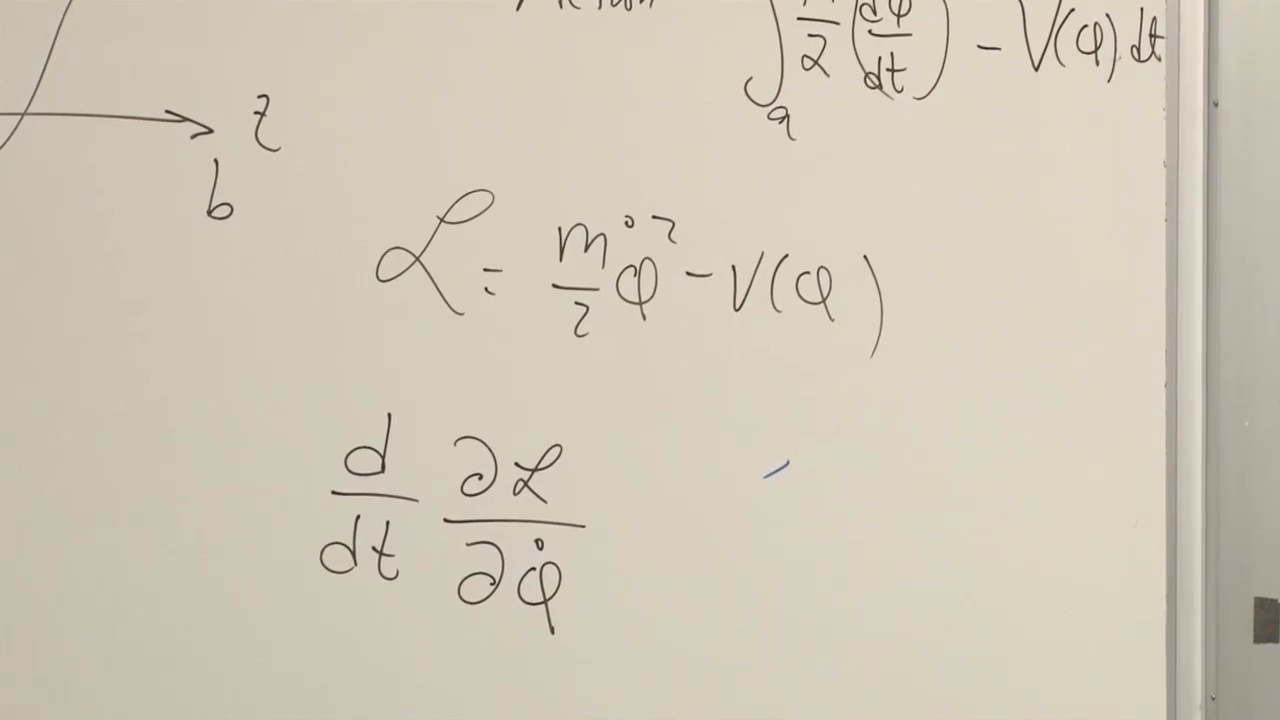
\includegraphics[width=0.90\textwidth]{lecture_04_figure_02.png}
\caption{표본화한 이력 \(\phi(t)\): 입자의 궤적이자, 새롭게 해석하면 \(0+1\)차원에서 장의 이력.}
\lectureframe{00:14:30}
\end{figure}

\begin{classroomqa}
\audiencequestion{공간 차원이 없으면 퍼텐셜은 사라지나요?}
\lecturerresponse{아닙니다. 공간적 변화는 사라져도 장에는 여전히 값이 있습니다. 에너지는 \(V(\phi)\)를 통해 그 값에 의존할 수 있습니다. 입자로 해석하면 곡선을 위아래로 옮길 때 퍼텐셜 에너지가 달라지고, 장으로 해석하면 서로 다른 \(\phi\) 값이 서로 다른 퍼텐셜 에너지를 갖습니다. \lecturetimestamp{00:15:00}}
\end{classroomqa}

\begin{classroomqa}
\audiencequestion{공간이 전혀 없는 경우 대신, 장이 시간에만 의존하는 보통의 공간을 상상해도 되나요?}
\lecturerresponse{네. 이 목적에서는 국소적인 수학이 같습니다. 모든 공간 미분이 사라지고 \(\phi(t)\)만 남습니다. 이를 \(0+1\)차원 이론이라고 부르면 축소된 구조를 분리해 볼 수 있지만, 더 큰 세계에서 공간적으로 균일한 장을 떠올려도 같은 직관을 얻을 수 있습니다. \lecturetimestamp{00:16:25}}
\end{classroomqa}

이 우회 과정의 요점이 이제 분명해졌다. 한 좌표인 시간에 의존하는 장에 대한 작용 원리를 알고 있다. 이 원리의 형태를 이용해 시공간의 모든 좌표에 의존하는 장의 작용 원리를 추측할 수 있다.

\section{시공간에 펼쳐진 장의 이력}

\subsection{곡선에서 곡면으로}

\(1+1\)차원에서 시공간 자체는 \(t\)와 \(x\)을 좌표로 하는 평면이다. 장의 값 \(\phi(x,t)\)은 세 번째 방향을 이룬다. 따라서 장의 이력은 곡선이 아니라 시공간 평면 위에 놓인 곡면이다. 스칼라장은 양수일 필요가 없으므로 곡면은 0보다 위로 솟거나 아래로 내려갈 수 있다.

\begin{figure}[htbp]
\centering
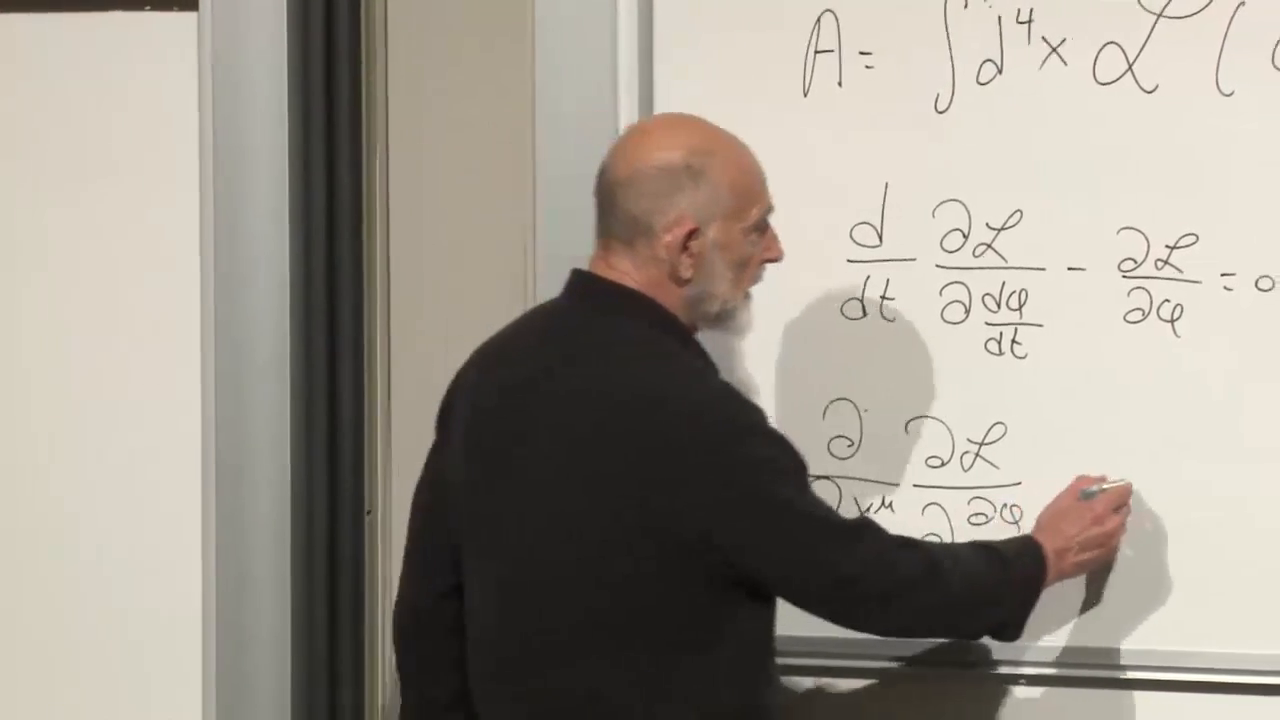
\includegraphics[width=0.90\textwidth]{lecture_04_figure_03.png}
\caption{\(1+1\)차원 시공간 평면 위의 곡면으로 나타낸 스칼라장의 이력.}
\lectureframe{00:20:46}
\end{figure}

우리의 물리적 시공간은 공간 3차원과 시간 1차원으로 이루어진 \(3+1\)차원 시공간이라고 부른다. 탁자 위의 모형은 \(2+1\)차원이고, 철사에 구슬을 꿰어 놓은 모습은 \(1+1\)차원의 세계를 떠올리게 한다. \(\phi\)을 그리려면 축 하나가 더 필요하므로 \(3+1\) 경우조차 충실하게 그릴 수는 없다. 하지만 정의는 명확하다. 완전한 이력은 모든 시공간 사건에 \(\phi\)의 값 하나를 대응시킨다.

\subsection{고정된 양 끝점에서 고정된 경계 자료로}

입자의 변분 문제에서는 양 끝점을 고정하고 그 사이의 곡선을 변분한다. 이에 대응하는 장론의 문제에서는 시공간 영역을 정하고 그 경계에서 \(\phi\)를 고정한 뒤 내부의 \(\phi\)를 변분한다. 그 영역은 \(1+1\)차원 그림의 직사각형일 수도 있고, 더 높은 차원의 시공간에 있는 적절한 임의의 영역일 수도 있다.

\begin{figure}[htbp]
\centering
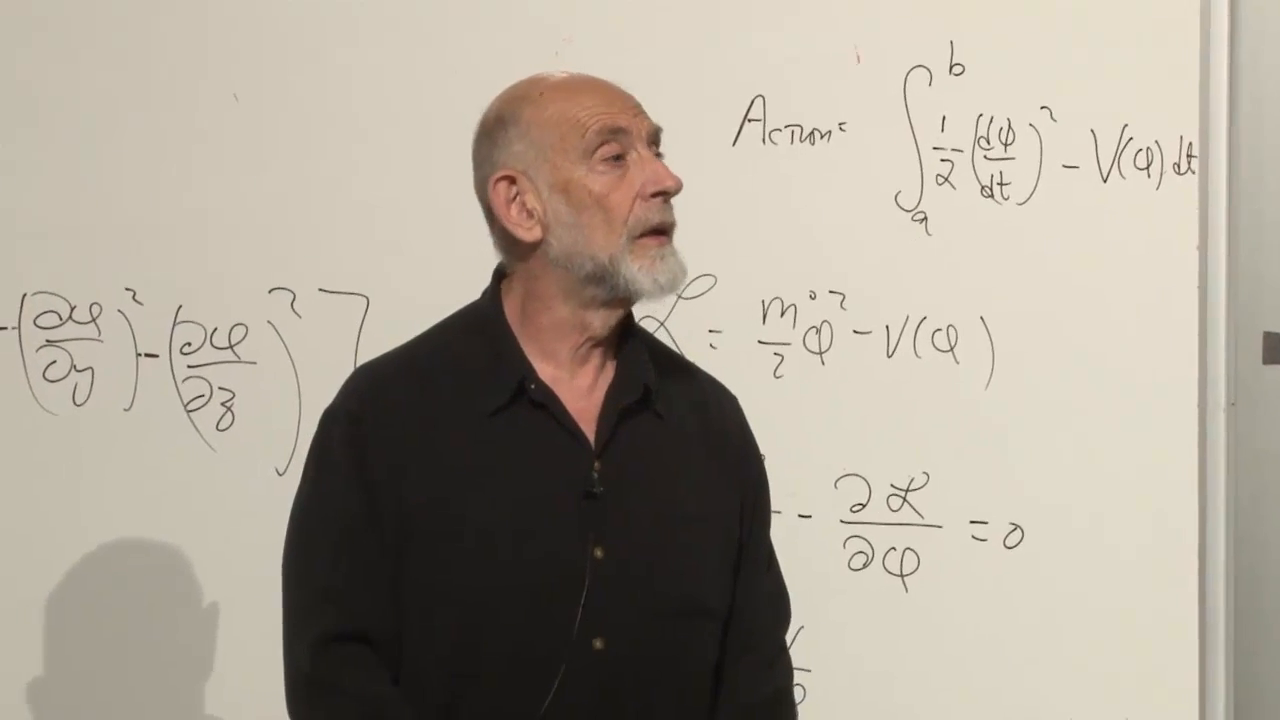
\includegraphics[width=0.90\textwidth]{lecture_04_figure_04.png}
\caption{시공간 영역의 경계 전체를 고정한 채 내부의 장을 변분한다.}
\lectureframe{00:24:52}
\end{figure}

\begin{classroomqa}
\audiencequestion{퍼텐셜이 시간에 명시적으로 의존해도 라그랑지언 정식화가 유효한가요?}
\lecturerresponse{네. 오일러--라그랑주 정식화와 해밀턴 정식화는 여전히 유효합니다. 일반적으로 사라지는 것은 에너지 보존입니다. 시간에 대한 명시적 의존성은 시간 병진 대칭성을 깨뜨립니다. 장론에서도 시공간에 대한 명시적 의존성을 허용할 수 있지만, 그에 따른 보존 법칙에 영향을 줍니다. \lecturetimestamp{00:23:49}}
\end{classroomqa}

\begin{classroomqa}
\audiencequestion{직사각형 모양의 장 영역에서는 위쪽과 아래쪽만 고정하나요, 아니면 경계 전체를 고정하나요?}
\lecturerresponse{이 변분 구성에서는 경계 전체를 고정합니다. \(1+1\)차원 직사각형의 네 변 모두를 고정합니다. 장은 내부에서만 요동할 수 있습니다. 이는 입자역학에서 양 끝점을 모두 고정하는 것에 직접 대응합니다. \lecturetimestamp{00:24:24}}
\end{classroomqa}

경계 전체를 고정한다는 것은 방정식을 유도할 때 사용하는 변분에 관한 설명이다. 이렇게 얻은 쌍곡형 장 방정식을 물리적 시간 진화 문제로 다룰 때는 적절한 초기 자료를 지정하고 방정식이 이를 미래로 전파하도록 두는 것이 더 일반적이다.

\section{작용과 장의 오일러--라그랑주 방정식}

\subsection{라그랑지언 밀도}

시공간 영역을 작은 셀들로 나누자. 작용은 각 셀의 국소적 기여를 모두 더한 값이라고 가정한다. 연속체 극한에서 그 합은 시공간 적분이 된다.
\begin{equation}
A[\phi]
=
\int_{\Omega} d^4x\,
\mathcal{L}\!\left(
\phi,\partial_\mu\phi;x^\mu
\right),
\qquad
d^4x=dt\,dx\,dy\,dz.
\label{eq:sr4-field-action}
\end{equation}
\(\mathcal{L}\)는 라그랑지언 밀도다. \(\mathcal{L}(\phi,\partial_\mu\phi;x^\mu)\)의 세미콜론은 역학적 논변과 좌표에 대한 명시적 의존 가능성을 구분한다. 균일한 폐쇄계에서는 보통 후자의 의존성이 없지만, 변분 형식은 이를 금하지 않는다.

간결한 표기
\begin{equation}
\partial_\mu\phi
\equiv
\frac{\partial\phi}{\partial x^\mu}
\end{equation}
는 시간 미분과 공간 미분을 한데 나타낸다. 강의의 성분 표기법으로는 다음과 같이 쓸 수도 있다.
\begin{equation}
\begin{aligned}
\phi_t&=\frac{\partial\phi}{\partial t},\\
\phi_x&=\frac{\partial\phi}{\partial x},\\
\phi_y&=\frac{\partial\phi}{\partial y},\\
\phi_z&=\frac{\partial\phi}{\partial z}.
\end{aligned}
\label{eq:sr4-component-derivatives}
\end{equation}
입자가 여러 좌표를 가질 수 있듯 장도 여러 개일 수 있다. 지금은 장이 \(\phi\) 하나뿐이다.

\(d^4x\)는 네 좌표에 대한 측도를 간략하게 쓴 기호일 뿐이다. 다른 차원의 시공간에서는 이를 \(d^Dx\)로 바꾸어야 한다. \(0+1\)차원 기본 모형에서는 \(D=1\)이고 \(d^1x\)는 그저 \(dt\)이다.

\begin{figure}[htbp]
\centering
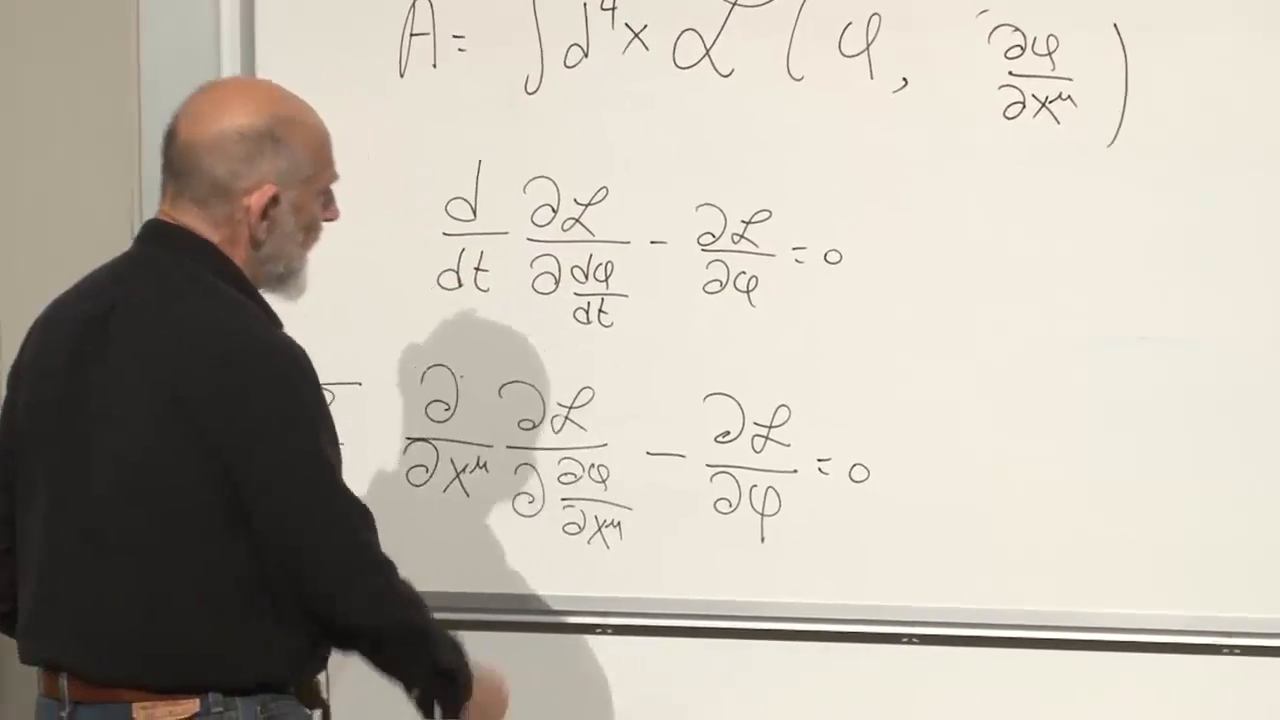
\includegraphics[width=0.90\textwidth]{lecture_04_figure_05.png}
\caption{국소 함수로 쓴 작용 밀도: \(\phi\)와 그 시공간 미분에 의존한다.}
\lectureframe{00:32:51}
\end{figure}

\begin{classroomqa}
\audiencequestion{라그랑지언 밀도도 \(x,y,z\) 자체에 의존할 수 있나요?}
\lecturerresponse{가능합니다. 입자 라그랑지언이 \(t\)에 명시적으로 의존할 수 있는 것과 같습니다. 병진 대칭인 폐쇄계에서는 보통 그렇지 않지만, 좌표에 명시적으로 의존해도 형식 자체는 유효합니다. \lecturetimestamp{00:30:29}}
\end{classroomqa}

\begin{classroomqa}
\audiencequestion{지금까지의 구성은 스칼라장에만 해당하나요, 아니면 일반적인가요?}
\lecturerresponse{지금까지의 변분 구조는 일반적입니다. 성분을 하나만 쓴 것은 스칼라장을 암시합니다. 벡터장이나 여러 장의 모음에는 성분 표지가 더 붙고, 각 성분을 모두 변분해야 합니다. \lecturetimestamp{00:31:00}}
\end{classroomqa}

\subsection{격자 모형}

촘촘한 시공간 격자에서는 미분이 이웃한 장 값 사이의 유한 차분이 된다. 그러면 작용은 여러 변수의 보통 함수가 된다. 한 방향에 점이 10개, 다른 방향에 점이 8개인 격자만으로도 장 변수는 이미 80개다. 격자를 세분할수록 변수의 수는 늘어나지만, 최소화 규칙은 여전히 간단하다. 내부의 각 점에서 장의 값에 대해 작용을 미분하고 그 결과를 0으로 둔다.

\begin{figure}[htbp]
\centering
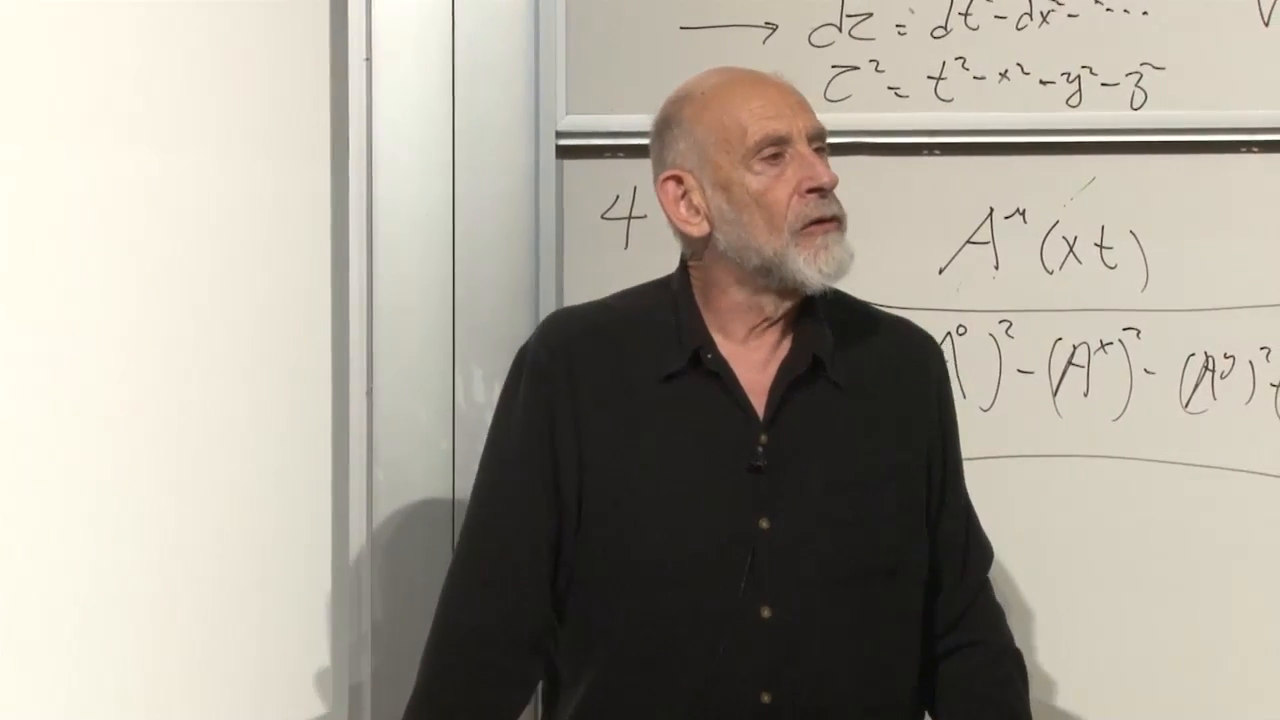
\includegraphics[width=0.90\textwidth]{lecture_04_figure_06.png}
\caption{시공간 영역을 셀들로 나누어, 연속체 극한을 취하기 전에 작용이 여러 변수의 보통 함수가 되도록 한 모습.}
\lectureframe{00:34:05}
\end{figure}

연속체 극한을 취하면 장의 오일러--라그랑주 방정식이 된다.
\begin{equation}
\boxed{
\partial_\mu
\left[
\frac{\partial\mathcal{L}}
{\partial(\partial_\mu\phi)}
\right]
-
\frac{\partial\mathcal{L}}{\partial\phi}
=0
}.
\label{eq:sr4-field-el}
\end{equation}
반복된 \(\mu\)는 모든 시공간 방향에 대해 합산한다. 합산 약식 없이 쓰면 같은 방정식은 다음과 같다.
\begin{align}
&
\frac{\partial}{\partial t}
\left(\frac{\partial\mathcal{L}}{\partial\phi_t}\right)
+
\frac{\partial}{\partial x}
\left(\frac{\partial\mathcal{L}}{\partial\phi_x}\right)
+
\frac{\partial}{\partial y}
\left(\frac{\partial\mathcal{L}}{\partial\phi_y}\right)
\nonumber\\
&\hspace{3em}
+
\frac{\partial}{\partial z}
\left(\frac{\partial\mathcal{L}}{\partial\phi_z}\right)
-
\frac{\partial\mathcal{L}}{\partial\phi}
=0.
\label{eq:sr4-field-el-expanded}
\end{align}
첫째 항은 익숙한 입자역학의 항이다. 장론에서는 각 공간 방향마다 이에 대응하는 항이 하나씩 추가된다. 마지막 항 \(-\partial\mathcal{L}/\partial\phi\)는 바뀌지 않는다.

\begin{figure}[htbp]
\centering
\includegraphics[width=0.90\textwidth]{lecture_04_figure_07.png}
\caption{1차원 오일러--라그랑주 방정식과 그 시공간 일반화를 위아래로 나란히 썼다.}
\lectureframe{00:38:44}
\end{figure}

이 분야는 연속체 역학이라고도 불린다. 자유도에 따라 같은 수학으로 유체 흐름, 탄성 변위 또는 다른 연속 매질을 기술할 수 있다.

\begin{classroomqa}
\audiencequestion{시간은 없고 공간만 있는 세계에서도 같은 방정식이 성립하나요?}
\lecturerresponse{네, 순수한 공간적 변분 문제로는 성립합니다. 물리적으로는 정적 해를 구할 때 이렇게 합니다. 장이 시간에 의존하지 않는다고 가정하고 시간 미분을 모두 버린 뒤 남은 공간 방정식을 풉니다. 시간에 따라 변하지 않는 전기장이나 자기장 구성이 그 예입니다. \lecturetimestamp{00:40:05}}
\end{classroomqa}

\section{가장 단순한 스칼라장 동역학 추측하기}

\subsection{부호가 모두 같을 수 없는 이유}

입자의 운동에너지 항 \(\tfrac12\dot\phi^2\)로 돌아가고, 중요하지 않은 전체 계수는 1로 두어 이를 일반화해 보자. 첫 추측은 다음과 같을 수 있다.
\begin{equation}
\mathcal{L}_{+}
=
\frac12
\left[
\phi_t^2+\phi_x^2+\phi_y^2+\phi_z^2
\right].
\label{eq:sr4-all-plus}
\end{equation}
이는 유용한 오답이다. 시간과 공간에 같은 부호를 부여하기 때문이다. 그 결과 얻는 방정식에는 파동 전파의 쌍곡형 구조가 나타나지 않는다. 올바른 상대론적 조합에서는 시간의 부호와 공간의 부호가 서로 반대다.

\begin{classroomqa}
\audiencequestion{모든 항의 부호가 같은 식이 틀린 것은 라그랑지언이 상대론적 불변량이어야 하기 때문인가요?}
\lecturerresponse{그것이 더 근본적인 답이며 옳습니다. 강의에서는 먼저 더 기초적인 방식으로 부호에 도달합니다. 파동은 시간에 따른 진화와 공간에 따른 변화를 구별하므로, 시간은 다른 공간 좌표와 완전히 같은 방식으로 들어갈 수 없습니다. 곧 로런츠 불변성이 이 직관을 정확한 규칙으로 만들어 줄 것입니다. \lecturetimestamp{00:43:19}}
\end{classroomqa}

특성 속도 \(c\)를 다시 포함하면 단순한 스칼라 라그랑지언 밀도는 다음과 같다.
\begin{equation}
\boxed{
\mathcal{L}
=
\frac12
\left[
\frac{1}{c^2}\phi_t^2
-\phi_x^2-\phi_y^2-\phi_z^2
\right]
-V(\phi)
}.
\label{eq:sr4-scalar-lagrangian}
\end{equation}
상대론적 장에서는 \(c\)가 빛의 속도다. 연속체 모형에서는 음속이나 탄성파의 속도 또는 다른 특성 전파 속도일 수도 있다.

전체 인자 \(1/2\)는 \(\tfrac12m\dot\phi^2\)에서와 마찬가지로 관례에 따른 것이다. 작용 전체에 0이 아닌 상수를 곱해도 정지 경로는 변하지 않는다. 이 관례에 따라 방정식에 쓰이는 매개변수의 이름과 정규화가 정해진다. 정규화를 정한 뒤에는 일관되게 사용해야 한다.

\begin{classroomqa}
\audiencequestion{공간 기울기 항을 퍼텐셜 에너지의 일부로 볼 수 있나요?}
\lecturerresponse{네. 운동에너지에서 퍼텐셜 에너지를 빼는 구성에서 운동에너지 부분에는 시간 미분이 들어간다. 공간 기울기 항과 \(V(\phi)\)를 포함해 시간 미분이 없는 항은 퍼텐셜 에너지 쪽에 속한다. 상대론적 이론에서 이 항들의 상대적 부호가 정해지는 궁극적인 이유는 로런츠 계량이다. \lecturetimestamp{00:45:37}}
\end{classroomqa}

\subsection{파동 방정식}

\eqref{eq:sr4-field-el}을 적용하자. 미분에 관한 항은 다음과 같다.
\begin{equation}
\frac{\partial\mathcal{L}}{\partial\phi_t}
=\frac{1}{c^2}\phi_t,
\qquad
\frac{\partial\mathcal{L}}{\partial\phi_i}
=-\phi_i,
\end{equation}
한편
\begin{equation}
\frac{\partial\mathcal{L}}{\partial\phi}
=-\frac{dV}{d\phi}.
\end{equation}
그러므로
\begin{equation}
\begin{aligned}
&\boxed{
\frac{1}{c^2}\frac{\partial^2\phi}{\partial t^2}
-\nabla^2\phi
+\frac{dV}{d\phi}
=0
},\\[0.5em]
\nabla^2
&=
\frac{\partial^2}{\partial x^2}
+\frac{\partial^2}{\partial y^2}\\
&\quad
+\frac{\partial^2}{\partial z^2}.
\end{aligned}
\label{eq:sr4-general-scalar-eom}
\end{equation}

\(V=0\)이면 다음과 같이 된다.
\begin{equation}
\boxed{
\frac{1}{c^2}\phi_{tt}-\nabla^2\phi=0
},
\label{eq:sr4-wave-equation}
\end{equation}
이것이 파동 방정식이다. 강의에서는 이 방정식을 알아보지만 풀이는 뒤로 미룬다. 이 방정식의 해는 속력 \(c\)으로 교란을 전파한다.

\begin{figure}[htbp]
\centering
\includegraphics[width=0.90\textwidth]{lecture_04_figure_08.png}
\caption{1차원 형태 \(c^{-2}\phi_{tt}-\phi_{xx}=0\)는 파동 방정식으로 알아볼 수 있다.}
\lectureframe{00:50:30}
\end{figure}

\subsection{결합된 조화 진동자로 이루어진 장}

이제 이차 퍼텐셜을 택하자.
\begin{equation}
V(\phi)=\frac12\mu^2\phi^2,
\qquad
\frac{dV}{d\phi}=\mu^2\phi.
\label{eq:sr4-quadratic-potential}
\end{equation}
\(\phi\)가 입자의 위치라면 이는 용수철 상수 \(\mu^2\)인 조화 진동자의 퍼텐셜이다. 장의 경우에는
\begin{equation}
\boxed{
\frac{1}{c^2}\phi_{tt}-\nabla^2\phi+\mu^2\phi=0
}.
\label{eq:sr4-klein-gordon}
\end{equation}
공간 미분을 빼면 이는 단순히 가속도에 상수와 변위를 곱한 항을 더해 0으로 놓은 식이다. 기울기 항이 이웃한 점들을 결합하여 진동자를 파동이 전파되는 연속체로 만든다. 상대론적 장론에서 \eqref{eq:sr4-klein-gordon}-- 방정식이라고 부른다. 고전적으로 \(\mu\)는 파동 전파를 수정하는 역길이 척도다.

\begin{figure}[htbp]
\centering
\includegraphics[width=0.90\textwidth]{lecture_04_figure_09.png}
\caption{이차 퍼텐셜과 복원항 \(\mu^2\phi\)이 들어간 결과 파동 방정식.}
\lectureframe{00:52:38}
\end{figure}

\begin{classroomqa}\audiencequestion{\(1/2\)는 \(V=\tfrac12\mu^2\phi^2\)에서 운동 방정식으로 넘어가면 왜 사라지는가?}\lecturerresponse{\(\phi^2\)을 미분하면 2라는 인자가 나온다. 관례에 따라 \(1/2\)을 넣는 것은 바로 \(dV/d\phi=\mu^2\phi\)가 되게 하기 위해서다. \(V(x)=\tfrac12kx^2\)가 복원력 \(-kx\)를 주는 것과 마찬가지다.\lecturetimestamp{00:53:17}}\end{classroomqa}

이 방정식은 선형이다. \(\phi\)와 그 미분이 모두 1차로만 나타난다. 운동 방정식에 \(\phi^2\)나 \(\phi\,\partial_\mu\phi\) 같은 항이 들어가면 동역학은 비선형이 된다.

\section{로런츠 스칼라와 사차원 벡터}

\subsection{작용은 기준계와 무관해야 한다}

변분 기법만으로도 여러 가능한 장 이론을 정의할 수 있다. 상대성 이론은 작용의 값과 형태가 모든 관성계에서 같아야 한다는 조건을 추가한다. 자유 입자에서는 세계선에 따라 불변 고유 시간 \(d\tau\)를 적분해 이를 만족시켰다. 장의 경우 작용은 시공간에 걸쳐 적분하므로 국소적인 구성 요소가 적절한 방식으로 변환되어야 한다.

정칙 로런츠 변환에서 시공간 측도는 불변이다.
\(d^4x'=d^4x\)
따라서 라그랑지언 밀도가 로런츠 스칼라가 되도록 요구하면 충분하다.
\begin{equation}
\mathcal{L}'(x')=\mathcal{L}(x).
\label{eq:sr4-lagrangian-scalar}
\end{equation}

\subsection{스칼라장}

스칼라장은 다음을 만족한다.
\begin{equation}
\boxed{\phi'(x')=\phi(x)}.
\label{eq:sr4-scalar-transform}
\end{equation}
좌표 \(x\)와 \(x'\)는 두 기준계에서 같은 사건을 표시한다. 관측자들이 사용하는 함수식은 달라 보일 수 있지만 그 물리적 사건에 붙는 수는 같다.

\begin{figure}[htbp]
\centering
\includegraphics[width=0.90\textwidth]{lecture_04_figure_10.png}
\caption{스칼라장의 정의 변환 법칙: \(\phi(x)=\phi'(x')\).}
\lectureframe{00:59:33}
\end{figure}

온도는 앞부분에서 직관을 얻는 데 쓰였지만, 물질 매질 속에서 움직이는 온도계는 완벽한 상대론적 사례가 아니다. 온도계 비유가 아니라 정의 \eqref{eq:sr4-scalar-transform}가 핵심이다.

\subsection{사차원 벡터}

단위계 \(c=1\)에서 \(v\)의 속도로 \(x\)축을 따라 가는 부스트는 다음과 같이 작용한다.
\begin{equation}
\begin{aligned}
t'&=\gamma(t-vx),\\
x'&=\gamma(x-vt),\\
y'&=y,\\
z'&=z,\\
\gamma&=\frac{1}{\sqrt{1-v^2}}.
\end{aligned}
\label{eq:sr4-x-boost}
\end{equation}

\begin{figure}[htbp]
\centering
\includegraphics[width=0.90\textwidth]{lecture_04_figure_11.png}
\caption{단위계 \(c=1\)에서 \(x\)축을 따라 가는 부스트에 대한 로런츠 변환.}
\lectureframe{01:02:26}
\end{figure}

부스트에 따라 서로 같은 방식으로 섞이는 네 물리량은 사차원 벡터를 이룬다. 지금까지 살펴본 예로는 \(x^\mu\), \(dx^\mu\), 사차원 속도 \(u^\mu=dx^\mu/d\tau\)가 있다. 사차원 벡터에 스칼라를 곱해도 사차원 벡터가 된다. 흐르는 상대론적 유체는 장으로 주어지는 예를 제공한다. 유체의 사차원 속도 \(u^\mu(x)\)는 사건에 따라 달라질 수 있다.

\eqref{eq:sr4-x-boost}와 같은 부스트에서 일반적인 사차원 벡터는 다음을 만족한다.
\begin{equation}
\begin{aligned}
A'^0&=\gamma(A^0-vA^x),\\
A'^x&=\gamma(A^x-vA^0),\\
A'^y&=A^y,\\
A'^z&=A^z.
\end{aligned}
\label{eq:sr4-vector-boost}
\end{equation}

일반적인 사차원 벡터 \(A^\mu=(A^0,A^x,A^y,A^z)\)에 대해 로런츠 놈
\begin{equation}
\boxed{
A_\mu A^\mu
=(A^0)^2-(A^x)^2-(A^y)^2-(A^z)^2
}
\label{eq:sr4-vector-norm}
\end{equation}
은 스칼라다. 이 값이 불변인 이유는 \begin{equation}
d\tau^2=dt^2-dx^2-dy^2-dz^2
\end{equation}가 불변인 이유와 같은 대수적 이유다. 강의에서는 일반 벡터를 나타낼 미사용 문자가 잠시 바닥나지만, 화살표를 연상시키는 제안 \(A\)을 받아 \(A\)를 사용한다.

\begin{figure}[htbp]
\centering
\includegraphics[width=0.90\textwidth]{lecture_04_figure_12.png}
\caption{일반적인 사차원 벡터장과 불변 놈을 이루는 로런츠 부호의 제곱 차.}
\lectureframe{01:09:06}
\end{figure}

\subsection{스칼라장의 미분}

스칼라장을 네 시공간 좌표에 대해 미분하면 다음 네 성분을 얻는다.
\begin{equation}
\partial_\mu\phi
=
\left(
\frac{\partial\phi}{\partial t},
\frac{\partial\phi}{\partial x},
\frac{\partial\phi}{\partial y},
\frac{\partial\phi}{\partial z}
\right)
\qquad(c=1).
\end{equation}
엄밀히 말해 \(\partial_\mu\phi\)는 공변 벡터다. 민코프스키 계량으로 지수를 올리면 \(\partial^\mu\phi\)가 된다. 여기서 성분을 사용한 논증에서는 이 구별이 문제가 되지 않지만, 수축을 명확히 정해 준다.
\begin{equation}
\boxed{
\partial_\mu\phi\,\partial^\mu\phi
=
\frac{1}{c^2}\phi_t^2
-\phi_x^2-\phi_y^2-\phi_z^2
}.
\label{eq:sr4-derivative-scalar}
\end{equation}

\begin{figure}[htbp]
\centering
\includegraphics[width=0.90\textwidth]{lecture_04_figure_13.png}
\caption{스칼라장의 일차 미분들로 구성한 불변 제곱 차.}
\lectureframe{01:13:55}
\end{figure}

\begin{classroomqa}
\audiencequestion{이 미분 조합이 라플라시안인가요?}
\lecturerresponse{아닙니다. 표시된 불변량은 일차 미분의 제곱으로 이루어져 있습니다. 라플라시안에는 이차 공간 미분이 들어갑니다. 이차 미분은 작용을 변분해 파동 방정식을 얻을 때 나타납니다. \lecturetimestamp{01:13:22}}
\end{classroomqa}

이제 \eqref{eq:sr4-scalar-lagrangian}의 부호 배열은 추측이 아니라 설명으로 정당화된다. 운동에너지와 기울기 항의 조합은 로런츠 스칼라 \(\partial_\mu\phi\,\partial^\mu\phi\)다. 따라서 가장 단순한 이차 이론은 다음과 같다.
\begin{equation}
\mathcal{L}
=
\frac12\partial_\mu\phi\,\partial^\mu\phi
-\frac12\mu^2\phi^2.
\label{eq:sr4-covariant-lagrangian}
\end{equation}

\begin{figure}[htbp]
\centering
\includegraphics[width=0.90\textwidth]{lecture_04_figure_14.png}
\caption{완성된 이차 스칼라장 라그랑지언과 그 선형 장 방정식.}
\lectureframe{01:19:12}
\end{figure}

\section{얼마나 많은 자유도가 있는가?}

스칼라를 만드는 규칙을 알면 가능한 라그랑지언은 많다. 장 \(\phi\)은 스칼라이므로 임의의 보통 함수 \(F(\phi)\)도 스칼라다. \(\phi^2\), \(\phi^3\), \(\cosh\phi\) 등이 그렇다. 수치 매개변수도 허용된다. \(\mu\) 같은 기호를 상수 계수로 넣을 수 있으며, 남는 문제는 그 차원과 물리적 의미뿐이다.

\begin{classroomqa}
\audiencequestion{라그랑지언에 질량을 넣을 수 있나요?}
\lecturerresponse{상수 매개변수는 당연히 넣을 수 있습니다. 이 단계에서는 어느 대상의 질량인지 물어야 합니다. 물리적 의미를 확인하기 전까지 \(\mu\)는 고전장론에서 단순한 수이기 때문입니다. 이차 상대론적 스칼라 이론에서는 질량 또는 역길이 척도를 정합니다. \lecturetimestamp{01:14:16}}
\end{classroomqa}

스칼라들을 곱할 수도 있다.
\begin{equation}
F(\phi)\,\partial_\mu\phi\,\partial^\mu\phi
\end{equation}
는 로런츠 불변량이다. 미분으로 만든 스칼라 자체를 제곱해 일차 미분의 고차 거듭제곱을 만들 수도 있다. 더 높은 차수의 미분도 고려할 수 있지만, 이 강의에서는 장과 그 일차 미분만 다룬다. 이것이 운동 방정식이 이차가 되는 표준적인 틀이다. 고차 미분 이론은 추가적인 동역학 자료와 불안정성이 일반적으로 생기므로 더 주의해서 다뤄야 한다.

\begin{classroomqa}
\audiencequestion{제곱 차로 만든 것이 정말 시공간의 계량인가요?}
\lecturerresponse{네. 선택한 부호 규약에서 계량은 \(dt^2-dx^2-dy^2-dz^2\)입니다. 강의에서 아직 계량이라는 말을 강조하지는 않았지만, 이는 일반상대성이론에서 핵심이 될 바로 그 시공간 기하다. \lecturetimestamp{01:19:39}}
\end{classroomqa}

\begin{classroomqa}
\audiencequestion{성분이 \(xy\)나 \(tx\)처럼 주어지는, 사차원 벡터보다 더 일반적인 대상도 있나요?}
\lecturerresponse{네. 그런 대상은 텐서입니다. 스칼라에는 시공간 지수가 없고, 벡터에는 하나 있으며, 이계 텐서에는 \(T^{xx}\), \(T^{xy}\), \(T^{tx}\) 같은 성분이 있습니다. 지금의 스칼라장 논의 대부분에서는 텐서를 피하지만, 일반상대성이론에서는 피할 수 없습니다. \lecturetimestamp{01:20:49}}
\end{classroomqa}

\begin{classroomqa}
\audiencequestion{왜 \(t\)와 \(x\)을 섞는 부스트만 다루나요? 다른 방향의 부스트는 공간축들을 다르게 섞을 수 있지 않나요?}
\lecturerresponse{물론입니다. \(y\) 방향의 부스트는 \(t\)와 \(y\)을 섞고 \(x,z\)은 그대로 둡니다. 일반적인 로런츠 변환은 공간 회전들과 선택한 축을 따른 부스트를 합성해 만들 수 있습니다. 따라서 회전 불변성과 표준 축 하나를 따른 부스트에 대한 불변성을 확인하면 충분합니다. \lecturetimestamp{01:22:06}}
\end{classroomqa}

\begin{classroomqa}
\audiencequestion{가능한 스칼라 조합이 이렇게 많은데, 그 결과로 얻는 라그랑지언이 모두 의미 있는 물리를 기술하나요?}
\lecturerresponse{고전 수준에서는 합리적인 부호, 국소성, 잘 정의된 시간 진화 문제 같은 추가 조건을 고려해도 자유도가 매우 큽니다. 잘 작동하는 기본 양자 이론을 정의하는 임의적 선택은 훨씬 적습니다. 현대 유효장론에서는 컷오프 아래에서 더 많은 상호작용을 허용하지만, 그때는 유효 범위를 명시해야 합니다. \lecturetimestamp{01:27:57}}
\end{classroomqa}

\begin{classroomqa}
\audiencequestion{장은 연속이어야 하나요?}
\lecturerresponse{여기서 다루는 매끄러운 이론에서는 그렇습니다. 불연속이 있으면 미분에 특이성이 생기고, 기울기의 제곱 항이 있으면 대개 작용과 에너지가 무한대가 됩니다. 더 특이한 형상은 추가적인 수학적 구조를 갖춰야만 다룰 수 있습니다. 여기서 전개하는 보통의 유한 에너지 장에는 해당하지 않습니다. \lecturetimestamp{01:29:29}}
\end{classroomqa}

\section{스칼라장과 결합한 입자}

\subsection{자유 입자를 다시 살펴보기}

강의의 마지막 부분에서는 고전적 수준에서 입자와 장을 함께 다룬다. 입자가 장의 들뜸이라는 양자적 설명을 다루는 단계는 아직 아니다. 대신 누군가 배경 스칼라장 \(\phi(x,t)\)을 이미 구했다고 가정하고, 입자가 그 장을 통과하며 어떻게 운동하는지 묻는다.

자유 상대론적 입자의 경우,
\begin{equation}
A_{\rm free}=-m\int d\tau.
\label{eq:sr4-free-particle-action}
\end{equation}
공간 차원이 1이고 \(c=1\)일 때,
\begin{equation}
d\tau=dt\sqrt{1-\dot x^2},
\qquad
L_{\rm free}=-m\sqrt{1-\dot x^2}.
\label{eq:sr4-free-particle-l}
\end{equation}
느린 속도로 전개했을 때 통상적인 양의 뉴턴역학적 운동에너지 항을 얻도록 마이너스 부호를 택한다:
\begin{equation}
L_{\rm free}
\approx -m+\frac12m\dot x^2+\cdots.
\end{equation}

\begin{figure}[htbp]
\centering
\includegraphics[width=0.90\textwidth]{lecture_04_figure_15.png}
\caption{불변인 자유 입자 작용을 좌표 시간에 대한 라그랑지언으로 다시 쓴 식.}
\lectureframe{01:34:31}
\end{figure}

\subsection{가장 간단한 스칼라 결합}

\(d\tau\)와 \(\phi\)는 모두 스칼라이다. 따라서 가장 간단한 선형 결합은 다음과 같다:
\begin{equation}
\boxed{
A
=
\int d\tau\,[-m+\phi(x,t)]
}.
\label{eq:sr4-coupled-action}
\end{equation}
이 선택이 유일한 것은 아니다. \(\phi\)를 임의의 함수 \(F(\phi)\)로 바꿀 수도 있다. 선형항만으로도 물리적 아이디어를 드러내기에 충분하다.

\begin{figure}[htbp]
\centering
\includegraphics[width=0.90\textwidth]{lecture_04_figure_16.png}
\caption{가장 간단한 로런츠 불변 스칼라 결합을 더한 자유 입자 작용.}
\lectureframe{01:37:21}
\end{figure}

\begin{classroomqa}
\audiencequestion{\(\phi\)는 적분 안에 계속 있어야 하나요?}
\lecturerresponse{그렇다. 장은 입자의 세계선 \(\phi(x(t),t)\)에서 평가되며, 궤적의 지점에 따라 일반적으로 값이 달라진다. 배경이 시간에 명시적으로 의존하지 않더라도, 즉 \(\phi=\phi(x)\)이더라도, 입자가 공간을 움직이면 시간에 따라 값이 변한다. 경로를 따라 일정한 장만 적분 밖으로 꺼낼 수 있다. \lecturetimestamp{01:37:47}}
\end{classroomqa}

\begin{classroomqa}
\audiencequestion{식 \(x\)의 \(\phi(x,t)\)는 입자의 위치를 뜻하나요?}
\lecturerresponse{그렇다. \(x=x(t)\)는 시간 \(t\)에서의 입자 위치이다. 작용은 주어진 시공간 장을 그 궤적을 따라 취한다. \lecturetimestamp{01:38:08}}
\end{classroomqa}

1차원 운동의 경우 \eqref{eq:sr4-coupled-action}는 다음을 준다.
\begin{equation}
L
=
-(m-\phi(x,t))\sqrt{1-\dot x^2}.
\label{eq:sr4-coupled-lagrangian}
\end{equation}
스칼라 배경은 정지 질량이 차지하던 바로 그 위치에 나타난다.
\begin{equation}
m_{\rm eff}(x,t)=m-\phi(x,t).
\label{eq:sr4-effective-mass}
\end{equation}
\(\phi\)가 거의 일정한 영이 아닌 값으로 수렴하면, 입자는 질량이 변한 것처럼 거동한다. 이는 완전한 힉스 메커니즘이 아니라 고전적인 장난감 모형일 뿐이지만, 힉스 아이디어의 핵심적인 특징, 즉 스칼라 배경이 질량항으로 입자 동역학에 들어갈 수 있다는 점을 잘 담아낸다.

\subsection{입자의 운동 방정식}

정준 운동량은 다음과 같다:
\begin{equation}
p
=
\frac{\partial L}{\partial\dot x}
=
(m-\phi)
\frac{\dot x}{\sqrt{1-\dot x^2}}.
\label{eq:sr4-coupled-momentum}
\end{equation}

\begin{figure}[htbp]
\centering
\includegraphics[width=0.90\textwidth]{lecture_04_figure_17.png}
\caption{스칼라 배경은 상대론적 정준 운동량에서 \(m\)을 \(m-\phi(x,t)\)로 대체한다.}
\lectureframe{01:43:38}
\end{figure}

라그랑지언을 위치에 대해 미분하면 다음과 같다:
\begin{equation}
\frac{\partial L}{\partial x}
=
\frac{\partial\phi}{\partial x}
\sqrt{1-\dot x^2}.
\end{equation}
작용 \eqref{eq:sr4-coupled-action}이 정하는 부호를 유지하면 오일러--라그랑주 방정식은 다음과 같다:
\begin{equation}
\boxed{
\frac{d}{dt}
\left[
(m-\phi)
\frac{\dot x}{\sqrt{1-\dot x^2}}
\right]
=
\frac{\partial\phi}{\partial x}
\sqrt{1-\dot x^2}
}.
\label{eq:sr4-coupled-eom}
\end{equation}

\begin{figure}[htbp]
\centering
\includegraphics[width=0.90\textwidth]{lecture_04_figure_18.png}
\caption{운동량과 배경장의 공간 미분으로 결합된 방정식을 세우며, 작용이 \eqref{eq:sr4-coupled-eom}의 최종 부호를 정한다.}
\lectureframe{01:45:24}
\end{figure}

\begin{classroomqa}
\audiencequestion{왜 \(\partial\phi/\partial x\)에는 \(\sqrt{1-\dot x^2}\) 인자가 남아 있나요?}
\lecturerresponse{\(\phi(x,t)\)에서 \(x\)에 대해 미분하는 것은 그 인자뿐이기 때문이다. 제곱근은 라그랑지언에서 그 인자에 곱해져 있으며, 편미분에서 \(\dot x\)를 고정하면 위치에 의존하지 않는다. 따라서 제곱근은 그대로 남는다. \lecturetimestamp{01:45:50}}
\end{classroomqa}

시간에 대한 전미분을 전개하면 다음과 같다:
\begin{align}
&(m-\phi)
\frac{d}{dt}
\left(
\frac{\dot x}{\sqrt{1-\dot x^2}}
\right)
-
\dot\phi\,
\frac{\dot x}{\sqrt{1-\dot x^2}}
\nonumber\\
&\hspace{10em}
=
\frac{\partial\phi}{\partial x}
\sqrt{1-\dot x^2}.
\label{eq:sr4-coupled-expanded}
\end{align}
배경이 정적이어서 \(\phi=\phi(x)\)이더라도, 움직이는 세계선을 따라 한 미분은 0이 아니다. 연쇄법칙을 적용하면 다음과 같다:
\begin{equation}
\boxed{
\dot\phi
=
\frac{d}{dt}\phi(x(t))
=
\frac{\partial\phi}{\partial x}\dot x
}.
\label{eq:sr4-chain-rule}
\end{equation}

\begin{classroomqa}
\audiencequestion{\(\phi\)에 시간에 대한 명시적 의존성이 없다면, 왜 \(\dot\phi\)는 0이 아닌가요?}
\lecturerresponse{입자의 위치가 변하기 때문이다. 장은 \(x(t)\)에서 취하므로 그 전미분은 \(\dot\phi=\phi_x\dot x\)이다. 정적 장이라는 말은 \(\partial\phi/\partial t=0\)라는 뜻이지, 움직이는 모든 입자가 일정한 장값을 경험한다는 뜻은 아니다. \lecturetimestamp{01:48:10}}
\end{classroomqa}

\begin{figure}[htbp]
\centering
\includegraphics[width=0.90\textwidth]{lecture_04_figure_19.png}
\caption{세계선을 따른 연쇄법칙을 적용한 뒤 결합 방정식을 전개한 마지막 단계.}
\lectureframe{01:49:11}
\end{figure}

정확한 식은 특별히 간결하지 않으며, 강의에서도 이를 감추려 하지 않는다. 그래도 저속 극한은 익숙한 형태를 갖는다. \(\sqrt{1-\dot x^2}\approx1\)이므로 선도 차수의 방정식은 다음과 같다:
\begin{equation}
\frac{d}{dt}\bigl[(m-\phi)\dot x\bigr]
\approx
\frac{\partial\phi}{\partial x}.
\end{equation}
유효 질량의 변화도 섭동으로 취급하면 다음 식을 얻는다:
\begin{equation}
(m-\phi)\ddot x
\approx
\frac{\partial\phi}{\partial x}.
\label{eq:sr4-nonrel-force}
\end{equation}
실제로 저속 라그랑지언은 다음과 같다:
\begin{equation}
L
\approx
-m+\phi+\frac12(m-\phi)\dot x^2,
\end{equation}
따라서 선도 차수에서 퍼텐셜 에너지는 \(U=-\phi\)이고 힘은 \(-dU/dx=\partial_x\phi\)이다. \(c\) 인자를 복원하여 이 뉴턴역학적 형태를 얻는 것으로 강의가 마무리된다.

입자에서 장으로 이어지는 과정이 이제 완결되었다. 입자의 이력 \(\phi(t)\)은 \(0+1\)차원 원형 모형을 제공했고, 장의 이력 \(\phi(x)\)은 작용을 시공간 적분으로 확장했다. 장의 오일러--라그랑주 방정식은 파동 동역학을 만들었고, 로런츠 스칼라는 상대론적 부호 구조를 정했다. 같은 불변 표현을 사용하면 스칼라 배경이 입자에 영향을 미치도록 할 수도 있었다.

\graphicspath{{../../../generated_course_notes/core/special_relativity/2012_spring_theoretical_minimum/chapters/lecture_05/}{../../../generated_course_notes/core/special_relativity/2012_spring_theoretical_minimum/figures/}{../../../generated_course_notes/core/special_relativity/2012_spring_theoretical_minimum/assets/}}
\chapter{입자, 장, 그리고 상대론적 표기법}

\section{강의에 앞서 다루는 도플러 편이 문제}

앞주 강의에서 남은 질문으로 논의를 시작한다. 빛의 속도에 가깝게 움직이는 관측자는 언제나 더 긴 파장을 측정할까? 그렇지는 않다. 답은 운동 방향에 달려 있다. 빛의 파동과 같은 방향으로 움직이는 관측자는 파장이 늘어나는 것을 보고, 파동과 반대 방향으로 움직이는 관측자는 파장이 짧아지는 것을 본다. 이것이 상대론적 도플러 효과다.

\begin{classroomqa}
\audiencequestion{빛의 속도에 가까운 운동은 관측되는 파장을 길게 만드는가?}
\lecturerresponse{관측자가 빛과 같은 방향으로 움직일 때만 그렇다. 관측자의 속도 방향을 반대로 바꾸면 편이 방향도 반대가 된다. 별도의 공식을 외우지 않고 로런츠 기하만으로 결과를 직접 구할 수 있다. \lecturetimestamp{00:00:13}}
\end{classroomqa}

단위계에서 \(c=1\)로 놓고, 프라임 좌표계가 속력 \(v\)로 오른쪽으로 움직인다고 하자. 오른쪽으로 진행하는 빛의 마루는 영 간격선을 따른다. 프라임이 없는 좌표계에서 파장을 1로 정규화하고, 연속하는 두 마루의 세계선을 다음과 같이 쓰자. \begin{equation}
x=t,
\qquad
x=t+1.
\label{eq:sr5-crest-lines}
\end{equation} 프라임이 없는 좌표계에서 파장은 \(t\)가 같은 순간에 두 마루 사이의 거리로 측정한다. 프라임 좌표계에서는 \(t'\)가 같은 순간에 두 마루 사이의 거리를 측정해야 한다. 따라서 계산의 핵심은 동시성의 상대성이다.

\begin{figure}[htbp]
\centering
\includegraphics[width=0.90\textwidth]{lecture_05_figure_01.png}
\caption{연속하는 오른쪽 진행 파동 마루, 빛원뿔, 그리고 움직이는 좌표계의 기울어진 축.}
\lectureframe{00:03:30}
\end{figure}

이 대목에서 강의 진행 순서에 관해 잠시 이야기한다. 여름 강의는 없다. 다음 강의 주제로는 일반상대성이론과 양자역학을 더 폭넓게 다시 다루는 방안이 모두 후보에 올라 있다. 양자장론을 공부하기 전에 조화진동자는 이해해 두어야 할 내용으로 특별히 언급된다.

\begin{classroomqa}
\audiencequestion{앞으로 적외선--자외선의 연결 관계를 다루는 강의가 있을까요?}
\lecturerresponse{그 질문은 양자역학과 중력의 접점에 속한다. 이 수업에서는 그 문제를 알아볼 만큼 양자역학을 다루지만, 먼저 중력을 전개해야 한다. 가장 자연스러운 출발점은 일반상대성이론이다. \lecturetimestamp{00:05:37}}
\end{classroomqa}

\begin{classroomqa}
\audiencequestion{기울어진 축 사이의 상대적 크기를 칠판 그림에서 눈대중으로 읽어도 될까요?}
\lecturerresponse{안 된다. 시공간 도표는 인과관계와 동시성의 기하를 나타내지만, 그림 위에서 보통의 유클리드 자로 잰 길이는 로런츠 측정값이 아니다. 관련 사건들을 정하고 로런츠 변환을 적용해야 한다. \lecturetimestamp{00:06:10}}
\end{classroomqa}

이제 계산을 이어가자. 프라임이 없는 좌표계에서 마루 사이의 간격을 1로 정규화하고, 대수적으로 프라임 좌표계에서 동시에 일어나는 두 사건을 찾는다.

로런츠 변환은 다음과 같다. \begin{equation}
t'=\gamma(t-vx),
\qquad
x'=\gamma(x-vt),
\qquad
\gamma=\frac{1}{\sqrt{1-v^2}}.
\label{eq:sr5-lorentz-doppler}
\end{equation} 프라임 좌표계의 동시성 단면을 \(t'=0\)로 택하자. 그러면 식 \eqref{eq:sr5-lorentz-doppler}에서 다음을 얻는다. \begin{equation}
t=vx.
\label{eq:sr5-primed-simultaneity}
\end{equation} 첫 번째 마루는 이 단면과 원점에서 만난다. 두 번째 마루는 \(x=t+1\)를 만족하므로, 교점은 다음 조건을 만족한다. \begin{align}
x&=vx+1,\\
x&=\frac{1}{1-v},
\qquad
t=\frac{v}{1-v}.
\end{align} 그 교점의 프라임 좌표는 다음과 같다. \begin{align}
x'
&=\frac{x-vt}{\sqrt{1-v^2}}\\
&=\frac{1-v^2}{(1-v)\sqrt{1-v^2}}\\
&=\sqrt{\frac{1+v}{1-v}}.
\end{align} 원래 파장이 1이었으므로, \begin{equation}
\boxed{
\frac{\lambda'}{\lambda}
=
\sqrt{\frac{1+\beta}{1-\beta}}
},
\qquad
\beta=\frac{v}{c}.
\label{eq:sr5-doppler}
\end{equation}이다. 이를 동치인 형태로 쓰면 다음과 같다. \begin{equation}
\frac{\lambda'}{\lambda}
=
\sqrt{\frac{c+v}{c-v}}.
\end{equation}

\begin{figure}[htbp]
\centering
\includegraphics[width=0.90\textwidth]{lecture_05_figure_02.png}
\caption{\(c\)를 복원한 도플러 인자. \(v\)의 방향을 반대로 하면 편이 인자는 역수가 된다.}
\lectureframe{00:13:40}
\end{figure}

\(v>0\)일 때 프라임 좌표계의 관측자는 빛을 따라가므로 더 긴 파장을 측정한다. \(v\)를 \(-v\)로 바꾸면 빛과 반대 방향으로 움직이는 경우가 되어 인자는 1보다 작아진다. 광선을 따라가며 관측자가 \(c\)에 가까워질 수 있다면 파장은 발산할 것이다. 진동수 편이는 그 비의 역수다.

\section{상호작용을 하나의 작용에 담아야 하는 이유}

도입 질문을 마치고 장과 입자를 다룬다. 양자장론에서는 결국 입자와 장이 동일한 들뜸을 기술하는 두 방식이 된다. 여기서는 그런 틀을 사용하지 않는다. 이 강의에서는 입자는 세계선을 따라가고 고전장은 시공간을 채운다. 당장 다룰 질문은 조금 더 소박하다. 장이 입자에 작용한다면, 입자는 어떻게 장에 되작용할까?

작용 원리는 유한 차원 모형을 통해 이 질문에 답한다. \(x(t)\)와 \(y(t)\)를 두 일반화 좌표라고 하자. 라그랑지안이 다음처럼 분리되면, \begin{equation}
L(x,\dot x,y,\dot y)
=
L_x(x,\dot x)+L_y(y,\dot y),
\label{eq:sr5-separable-l}
\end{equation} 두 오일러--라그랑주 방정식은 서로 독립이다. \begin{equation}
\frac{d}{dt}\frac{\partial L}{\partial\dot x}
=
\frac{\partial L}{\partial x},
\qquad
\frac{d}{dt}\frac{\partial L}{\partial\dot y}
=
\frac{\partial L}{\partial y}.
\end{equation} \(x\) 방정식에는 \(y\)가 들어 있지 않고, \(y\) 방정식에는 \(x\)가 들어 있지 않다.

두 변수를 상호작용시키려면 \(x\)에 관한 항과 \(y\)에 관한 항으로 분리할 수 없는 항을 더하면 된다. 간단한 예는 다음과 같다. \begin{equation}
L
=
\frac{\dot x^2}{2}
+\frac{\dot y^2}{2}
-V(x)-W(y)+\kappa xy.
\label{eq:sr5-coupled-coordinates}
\end{equation} 이제 \(x\)를 변분하면 \(y\)에 비례하는 항이 나오고, \(y\)을 변분하면 \(x\)에 비례하는 항이 나온다. 두 작용 방향 모두를 지배하는 것은 같은 혼합항이다.

\begin{figure}[htbp]
\centering
\includegraphics[width=0.90\textwidth]{lecture_05_figure_03.png}
\caption{라그랑지안의 한 항에 두 일반화 좌표가 함께 들어 있으면 두 좌표는 동역학적으로 결합된다.}
\lectureframe{00:19:00}
\end{figure}

여기서 사용하는 작용--반작용 진술이 정확히 성립하는 조건은 이렇다. 두 대상이 모두 동역학적 변수이고, 하나의 공통 작용을 두 대상에 대해 모두 변분한다. 장을 외부에서 주어진 배경으로 취급하면 장의 반응이 드러나지 않을 수 있다. 하지만 장 자체를 동역학적으로 다루면 결합항이 두 방정식을 모두 만든다.

\section{스칼라장이 입자에 작용하는 방식}

\subsection{상대론적 결합}

먼저 스칼라장 \(\phi(\mathbf{x},t)\)가 알려져 있다고 하자. 파동일 수도 있고 정적인 분포일 수도 있다. 지금은 장 자체의 방정식을 고려하지 않는다. 자유 상대론적 입자의 작용은 다음과 같다. \begin{equation}
S_{\mathrm p}
=
-m\int d\tau.
\end{equation} 직선 위의 운동에 대해 \(c=1\)로 놓으면, \begin{equation}
L_{\mathrm p}^{(0)}
=
-m\sqrt{1-\dot x^2}.
\end{equation}이다. 가장 간단한 스칼라 결합은 질량 계수를 장에 의존하는 양으로 바꾸는 것이다. \begin{equation}
\boxed{
L_{\mathrm p}
=
-\bigl[m+g\phi(x,t)\bigr]\sqrt{1-\dot x^2}
}.
\label{eq:sr5-particle-coupling}
\end{equation} 결합 상수 \(g\)는 장이 이 입자에 미치는 영향의 세기를 나타낸다. 부호는 관례에 따라 정한다. \(g\)를 \(-g\)로 바꾸면 스칼라 힘의 방향이 반대가 된다.

\begin{figure}[htbp]
\centering
\includegraphics[width=0.90\textwidth]{lecture_05_figure_04.png}
\caption{\(m\)를 국소 계수 \(m+g\phi(x,t)\)로 바꾼 자유 입자 작용.}
\lectureframe{00:24:10}
\end{figure}

\subsection{저속 입자 극한}

뉴턴 극한이 드러나도록 빛의 속도를 다시 표시하자. \begin{equation}
L_{\mathrm p}
=
-\bigl[mc^2+g\phi(x,t)\bigr]
\sqrt{1-\frac{\dot x^2}{c^2}}.
\label{eq:sr5-particle-coupling-c}
\end{equation} \(|\dot x|\ll c\)일 때는, \begin{equation}
\sqrt{1-\frac{\dot x^2}{c^2}}
=
1-\frac{\dot x^2}{2c^2}
+O\!\left(\frac{\dot x^4}{c^4}\right).
\end{equation}이다. 이를 \eqref{eq:sr5-particle-coupling-c}에 대입하면 다음과 같다. \begin{align}
L_{\mathrm p}
&=
-mc^2-g\phi
+\frac{m\dot x^2}{2}
+\frac{g\phi\,\dot x^2}{2c^2}
+O(c^{-4})\\
&\longrightarrow
\frac{m\dot x^2}{2}-g\phi(x,t),
\label{eq:sr5-nr-particle}
\end{align} 상수항 \(-mc^2\)과 \(c^{-2}\)만큼 작은 항을 버리면 얻는 결과는 보통의 형태 \(T-V\)이므로, \begin{equation}
V_{\mathrm p}(x,t)=g\phi(x,t).
\label{eq:sr5-scalar-potential}
\end{equation}이다.

\begin{figure}[htbp]
\centering
\includegraphics[width=0.90\textwidth]{lecture_05_figure_05.png}
\caption{제곱근을 전개하면 뉴턴 역학의 운동에너지 항과 스칼라 퍼텐셜 에너지 \(g\phi\)가 남는다.}
\lectureframe{00:28:50}
\end{figure}

큰 정지 에너지 상수는 오일러--라그랑주 방정식에 들어가지 않는다. 장에 의존하는 항은 방정식에 영향을 준다. 전자기학에서는 전하가 이와 비슷한 결합 세기 역할을 하지만, 실제 전자기 상호작용에는 이 스칼라 모형이 아니라 사벡터 퍼텐셜이 쓰인다.

\section{입자가 장에 되작용하는 방식}

\subsection{하나의 변분 문제}

이제 장을 단지 주어진 것으로 둘 수는 없다. 장의 배치와 입자 세계선이 함께 들어 있는 시공간 영역을 생각하자. 두 가지 모두에 대한 변분에서 전체 작용이 정지할 때 물리적 해를 얻는다. \begin{equation}
\delta S[\phi,x]=0.
\end{equation} 장을 고정한 채 세계선을 변분하면 입자 방정식을 얻는다. 세계선을 고정한 채 장을 변분하면 장 방정식을 얻는다. 두 방정식을 이어 주는 것은 두 방정식에 공통으로 들어가는 상호작용항이다.

\begin{figure}[htbp]
\centering
\includegraphics[width=0.90\textwidth]{lecture_05_figure_06.png}
\caption{스칼라장이 차지한 시공간 영역을 지나는 입자의 세계선.}
\lectureframe{00:30:30}
\end{figure}

질량이 없는 자유 스칼라장에 대해 다음과 같이 두자. \begin{equation}
S_{\mathrm f}
=
\int d^4x\,
\frac12
\left[
(\partial_t\phi)^2
-(\partial_x\phi)^2
-(\partial_y\phi)^2
-(\partial_z\phi)^2
\right].
\label{eq:sr5-free-field-action}
\end{equation} 여기서부터 다시 \(c=1\)를 사용한다. 단위를 명시하면 좌표와 장을 어떻게 정규화하느냐에 따라 시간 항에 그에 맞는 \(1/c^2\) 인자가 들어간다.

\begin{figure}[htbp]
\centering
\includegraphics[width=0.90\textwidth]{lecture_05_figure_07.png}
\caption{입자 세계선과 같은 시공간 영역에 걸쳐 쓴 장의 작용.}
\lectureframe{00:32:10}
\end{figure}

\subsection{정지한 입자와 세계선 적분}

대수를 최소화하면서 원천항을 드러내기 위해 입자를 원점에 정지시켜 두자. 그러면 인자 \(d\tau\)는 \(dt\)와 같고, \eqref{eq:sr5-particle-coupling}의 상호작용 부분은 다음과 같이 된다. \begin{equation}
S_{\mathrm{int}}
=
-g\int dt\,\phi(\mathbf{0},t).
\label{eq:sr5-worldline-interaction}
\end{equation} 이것은 세계선을 따라서만 적분하는 반면, \eqref{eq:sr5-free-field-action}는 전체 시공간에 걸쳐 적분한다. 둘을 하나의 시공간 적분으로 합치려면 입자의 위치를 선택하는 함수가 필요하다.

\begin{figure}[htbp]
\centering
\includegraphics[width=0.90\textwidth]{lecture_05_figure_08.png}
\caption{장 영역 안에 있는 정지 세계선과, 이 세계선과 합쳐야 하는 장의 작용.}
\lectureframe{00:35:35}
\end{figure}

\subsection{디랙 델타 함수}

일차원 델타 함수는 다음과 같이 정의된다.
\begin{equation}
\int_{-\infty}^{\infty}dx\,f(x)\delta(x-a)=f(a).
\label{eq:sr5-delta-definition}
\end{equation}
\(x=a\)에서 벗어나면 0이고, \(x=a\)에서 특이하며, 적분하면 단위값을 갖는다.
이 함수는 보통의 유한한 값을 갖는 함수라기보다 다음 관계로 특징지어지는 분포로 이해하는 것이 가장 적절하다.
\eqref{eq:sr5-delta-definition}

\begin{figure}[htbp]
\centering
\includegraphics[width=0.90\textwidth]{lecture_05_figure_09.png}
\caption{원점에서의 장 값을 공간 적분으로 바꾸는 델타 함수 항등식.}
\lectureframe{00:36:45}
\end{figure}

3차원에서는, \begin{equation}
\delta^3(\mathbf{x})
=
\delta(x)\delta(y)\delta(z),
\end{equation}이므로 다음이 성립한다. \begin{align}
\int d^3x\,
\phi(\mathbf{x},t)\delta^3(\mathbf{x})
&=
\int dx\,dy\,dz\,
\phi(x,y,z,t)\\
&\quad\times\delta(x)\delta(y)\delta(z)\\
&=\phi(\mathbf{0},t).
\label{eq:sr5-triple-delta}
\end{align}

\begin{classroomqa}
\audiencequestion{\(d^3x\)는 어디에서 나오는가?}
\lecturerresponse{보통의 공간 부피 요소 \(dx\,dy\,dz\)이다. 공간 차원이 1차원이면 같은 항등식에는 \(dx\)와 델타 함수 하나만 들어간다. \lecturetimestamp{00:37:09}}
\end{classroomqa}

\begin{figure}[htbp]
\centering
\includegraphics[width=0.90\textwidth]{lecture_05_figure_10.png}
\caption{3차원 델타 함수를 1차원 인자 세 개로 전개한 모습.}
\lectureframe{00:39:05}
\end{figure}

이제 식 \eqref{eq:sr5-worldline-interaction}을 다음처럼 쓸 수 있다. \begin{equation}
S_{\mathrm{int}}
=
-g\int d^4x\,
\delta^3(\mathbf{x})\phi(\mathbf{x},t).
\end{equation} 정지한 원천을 포함한 전체 작용은 다음과 같다. \begin{align}
S
=
\int d^4x
\biggl\{
&\frac12(\partial_t\phi)^2
-\frac12|\boldsymbol{\nabla}\phi|^2
\nonumber\\
&-g\delta^3(\mathbf{x})\phi
\biggr\}.
\label{eq:sr5-combined-action}
\end{align}

\begin{classroomqa}
\audiencequestion{상호작용을 시공간 작용에 넣을 때 마이너스 부호를 빠뜨린 건가요?}
\lecturerresponse{세계선 라그랑지안에는 \(-g\phi\)가 들어 있으므로, 시공간 라그랑지안 밀도에는 \(-g\delta^3(\mathbf{x})\phi\)가 들어가야 한다. 이 부호를 유지해야 장 방정식의 원천항 부호가 정해진다. \lecturetimestamp{00:41:24}}
\end{classroomqa}

\begin{figure}[htbp]
\centering
\includegraphics[width=0.90\textwidth]{lecture_05_figure_11.png}
\caption{자유 스칼라장 밀도와 국소화된 상호작용을 하나의 시공간 작용으로 합친 모습.}
\lectureframe{00:42:05}
\end{figure}

\subsection{원천이 있는 장 방정식}

\eqref{eq:sr5-combined-action}을 \(\phi\)에 대해 변분하면 다음을 얻는다. \begin{equation}
\boxed{
\partial_t^2\phi-\nabla^2\phi
=
-g\delta^3(\mathbf{x})
}.
\label{eq:sr5-sourced-wave}
\end{equation} 원점에서 떨어진 곳에서는 자유 파동 방정식이다. 원점에서는 델타 함수가 입자를 국소화된 원천으로 나타낸다.

\begin{figure}[htbp]
\centering
\includegraphics[width=0.90\textwidth]{lecture_05_figure_12.png}
\caption{원점의 점 원천이 구동하는 파동 연산자.}
\lectureframe{00:45:35}
\end{figure}

정적 해에서는 \(\partial_t\phi=0\)이므로, \begin{equation}
\boxed{
\nabla^2\phi
=
g\delta^3(\mathbf{x})
}.
\label{eq:sr5-poisson}
\end{equation}이다. 이것은 점 원천에 대한 푸아송 방정식이다. 여기서의 비유는 정전기학에 해당하며, 아직 전자기학은 아니다. 장은 여전히 스칼라 \(\phi\)이지 전자기 사퍼텐셜이 아니다.

\begin{figure}[htbp]
\centering
\includegraphics[width=0.90\textwidth]{lecture_05_figure_13.png}
\caption{원천이 있는 파동 방정식의 정적 극한. 이 식은 푸아송 방정식이다.}
\lectureframe{00:47:05}
\end{figure}

이제 상호성이 명확해졌다. 항 \(g\phi\)은 입자에 퍼텐셜 에너지를 주고, 같은 \(g\)는 입자를 \(\phi\)의 원천으로 만든다. 이 두 효과를 서로 독립적인 가정으로 두는 것이 아니다.

\subsection{움직이는 원천은 복사한다}

\(\mathbf{a}\)에 고정된 입자는 \(\delta^3(\mathbf{x}-\mathbf{a})\)로 나타낸다. 입자의 위치가 시간에 따라 변하면 원천은 다음과 같이 된다. \begin{equation}
\delta^3\!\left(\mathbf{x}-\mathbf{a}(t)\right).
\label{eq:sr5-moving-delta}
\end{equation} 시간에 따라 변하는 우변은 시간에 무관한 장으로 상쇄할 수 없다. 따라서 \(\partial_t^2\phi\) 항이 다시 필요하고, 가속하거나 진동하는 원천은 장에 파동을 일으킬 수 있다.

\begin{figure}[htbp]
\centering
\includegraphics[width=0.90\textwidth]{lecture_05_figure_14.png}
\caption{\(\mathbf{a}(t)\)로 옮겨 간 델타 함수 원천. 이에 따라 장 방정식은 시간에 의존한다.}
\lectureframe{00:50:30}
\end{figure}

\begin{classroomqa}
\audiencequestion{원천을 비상대론적으로 다룬다면 장 방정식에서 상대론은 어디에 들어 있나요?}
\lecturerresponse{왼쪽의 시공간 파동 연산자에 상대론적 전파가 담겨 있다. 입자까지 완전히 상대론적으로 다루면 고유시간 작용과 속도 인자를 유지해야 한다. 느리게 움직이는 원천이라도 시간에 따라 변하면 파동을 일으킬 수 있다. \lecturetimestamp{00:52:14}}
\end{classroomqa}

\begin{classroomqa}
\audiencequestion{\(g\phi\)의 단위는 무엇인가요?}
\lecturerresponse{입자 작용에서 \(mc^2\)와 나란히 나타나므로 에너지 단위를 갖는다. 여기서 사용하는 자연 단위 정규화에서는 \(3+1\)차원 스칼라의 질량 차원이 1이고 \(g\)는 무차원일 수 있다. 차원은 시공간 차원과 장의 정규화에 따라 달라진다. \lecturetimestamp{00:52:55}}
\end{classroomqa}

\section{사벡터, 스칼라, 그리고 계량}

성분 방정식이 길어져 더 나은 표기법이 필요해졌다. 시공간 좌표를 다음과 같이 쓰자. \begin{equation}
x^\mu=(x^0,x^1,x^2,x^3)=(t,x,y,z),
\label{eq:sr5-four-coordinate}
\end{equation} 여기서 그리스 지표는 네 성분 전체를 돈다. 네 성분으로 된 목록이라고 해서 저절로 사벡터가 되는 것은 아니다. 성분들이 \(x^\mu\)와 같이 로런츠 변환에 따라 변환할 때만 사벡터다.

\begin{figure}[htbp]
\centering
\includegraphics[width=0.90\textwidth]{lecture_05_figure_15.png}
\caption{네 시공간 좌표를 \(x^\mu\)로 모아 쓴 모습.}
\lectureframe{00:55:00}
\end{figure}

공간 성분 전체가 0이라는 진술은 한 기준계에서는 성립하지만 다른 기준계에서는 성립하지 않을 수 있다. 반면 모든 성분이 0이면 모든 로런츠 관측자가 그 벡터가 영벡터라는 데 동의한다. \(dx^\mu\)와 같은 차분도 사차원 벡터이다.

불변 고유시간 간격은 다음과 같다. \begin{equation}
d\tau^2
=
dt^2-dx^2-dy^2-dz^2.
\label{eq:sr5-proper-time}
\end{equation} 이는 좌표계에 따라 달라지는 네 성분을 갖는 것이 아니라 하나의 값만 가지므로 스칼라다.

\begin{figure}[htbp]
\centering
\includegraphics[width=0.90\textwidth]{lecture_05_figure_16.png}
\caption{사변위와 불변 고유시간 간격.}
\lectureframe{00:57:25}
\end{figure}

\subsection{민코프스키 계량}

시간 성분의 부호가 음수인 계량 부호 규약을 채택하자. \begin{equation}
\eta_{\mu\nu}
=
\operatorname{diag}(-1,1,1,1).
\label{eq:sr5-metric}
\end{equation} 공간 성분의 부호가 음수인 규약도 똑같이 타당하지만, 모든 방정식에서 한 가지 규약을 일관되게 써야 한다. \eqref{eq:sr5-metric}를 사용하면, \begin{equation}
dx^\mu dx_\mu
=
-dt^2+dx^2+dy^2+dz^2
=
-d\tau^2.
\end{equation}이다. 전체 부호는 불변성에 영향을 주지 않는다.

\begin{figure}[htbp]
\centering
\includegraphics[width=0.90\textwidth]{lecture_05_figure_17.png}
\caption{시간 성분의 부호가 음수인 민코프스키 계량을 대각 행렬로 쓴 모습.}
\lectureframe{01:00:30}
\end{figure}

계량은 지표를 내린다. \begin{equation}
A_\mu=\eta_{\mu\nu}A^\nu.
\label{eq:sr5-lower-index}
\end{equation} 이 데카르트 계량에서는, \begin{equation}
A^\mu=(A^0,A^1,A^2,A^3),
\qquad
A_\mu=(-A^0,A^1,A^2,A^3).
\label{eq:sr5-upper-lower-components}
\end{equation}이다. \(\eta^{\mu\rho}\eta_{\rho\nu}=\delta^\mu{}_\nu\)이므로 같은 계량을 한 번 더 적용하면 지표를 올린다.

\begin{figure}[htbp]
\centering
\includegraphics[width=0.90\textwidth]{lecture_05_figure_18.png}
\caption{행렬 \(\eta_{\mu\nu}\)를 곱해 지표를 내리는 과정.}
\lectureframe{01:03:00}
\end{figure}

\begin{classroomqa}
\audiencequestion{여기서 보통의 행렬 곱셈에도 정말 합이 들어 있나요?}
\lecturerresponse{그렇다. 각 출력 성분은 \(\eta\)의 한 행과 전체 벡터를 곱한 것이며, 열 지표에 대해 합한다. 대각 계량에서는 계산이 자명해 보이지만, 일반 행렬에서는 그 합이 명시적으로 드러난다. \lecturetimestamp{01:04:56}}
\end{classroomqa}

\subsection{아인슈타인 합산 규약과 자유 지표}

아인슈타인 합산 규약에서는 지표가 한 번은 위에, 한 번은 아래에 반복되면 합 기호를 생략한다. \begin{equation}
\eta_{\mu\nu}A^\nu
\equiv
\sum_{\nu=0}^{3}\eta_{\mu\nu}A^\nu.
\end{equation} 여기서 \(\nu\)는 더미 지표다. 이 지표는 합산되어 사라지므로 이름을 바꿔도 된다. 지표 \(\mu\)는 자유 지표로, 결과의 네 성분을 가리킨다. 보통 하나의 단항식에서 같은 지표가 세 번 이상 나타나면 안 된다.

전통적인 명칭은 위 지표를 \emph{반변}, 아래 지표를 \emph{공변}이라 한다. 이 강의에서는 일부러 더 쉬운 표현인 \emph{위}와 \emph{아래}를 선호하지만, 두 용어는 같은 변환 규칙을 가리킨다.

\section{수축과 스칼라의 미분}

\subsection{민코프스키 내적}

벡터와 그 지표를 내린 벡터를 수축하면 다음을 얻는다. \begin{equation}
A^\mu A_\mu
=
\eta_{\mu\nu}A^\mu A^\nu
=
-(A^0)^2+(A^1)^2+(A^2)^2+(A^3)^2.
\label{eq:sr5-vector-square}
\end{equation} 마이너스 부호를 따로 더해서는 안 된다. 그 부호는 이미 지표를 내린 시간 성분에서 나온다.

\begin{figure}[htbp]
\centering
\includegraphics[width=0.90\textwidth]{lecture_05_figure_19.png}
\caption{시간 성분과 공간 성분으로 전개한 수축 \(A^\mu A_\mu\).}
\lectureframe{01:09:30}
\end{figure}

\begin{classroomqa}
\audiencequestion{아래 지표 벡터는 행벡터로 그려야 하나요?}
\lecturerresponse{초등적인 행렬 표기에서는 행벡터로 나타낼 수 있지만, 지표 표기법은 그런 선택을 요구하지 않는다. 그 벡터를 규정하는 것은 변환 방식과 위 지표 벡터와의 수축 방식이다. \lecturetimestamp{01:10:26}}
\end{classroomqa}

\begin{classroomqa}
\audiencequestion{그리스 지표는 언제나 네 성분 모두를 가리키나요?}
\lecturerresponse{이 표기법에서는 그렇다. \(\mu,\nu\)와 같은 그리스 지표는 시공간 성분을 도는 반면, \(i,j\)와 같은 라틴 지표는 대개 공간 성분 세 개만 돈다. \lecturetimestamp{01:12:23}}
\end{classroomqa}

서로 다른 두 사벡터에도 같은 구성이 성립한다. \begin{equation}
A^\mu B_\mu
\end{equation}는 스칼라다. 간단히 보이는 증명에는 편극 항등식을 쓸 수 있다. \((A+B)^2\)와 \((A-B)^2\)가 모두 스칼라이므로, \begin{equation}
(A+B)^2-(A-B)^2=4A^\mu B_\mu
\end{equation}도 스칼라다. 이는 보통의 내적에 해당하는 민코프스키 공간의 식이다.

\begin{classroomqa}
\audiencequestion{\(A^\mu B_\mu\)는 보통의 내적과 비슷한가요?}
\lecturerresponse{그렇다. 민코프스키 계량이 시간 성분과 공간 성분 사이의 상대적인 부호를 정한다는 점만 다르다. \lecturetimestamp{01:15:44}}
\end{classroomqa}

\subsection{기울기는 공변벡터다}

\(\phi(x)\)를 스칼라장이라 하고, 여기서 \(x\)는 네 시공간 좌표 전체를 나타낸다고 하자. 이웃한 사건들 사이에서, \begin{equation}
d\phi
=
\frac{\partial\phi}{\partial x^\mu}dx^\mu
=
\partial_\mu\phi\,dx^\mu.
\label{eq:sr5-dphi}
\end{equation}이다. 좌변은 스칼라이고 \(dx^\mu\)는 사벡터다. 따라서 계수 \begin{equation}
\partial_\mu\phi
=
\left(
\partial_t\phi,
\partial_x\phi,
\partial_y\phi,
\partial_z\phi
\right)
\label{eq:sr5-gradient-lower}
\end{equation}는 공변벡터처럼 변환해야 한다. 지표를 올리면 다음과 같다. \begin{equation}
\partial^\mu\phi
=
\left(
-\partial_t\phi,
\partial_x\phi,
\partial_y\phi,
\partial_z\phi
\right).
\label{eq:sr5-gradient-upper}
\end{equation}

\begin{figure}[htbp]
\centering
\includegraphics[width=0.90\textwidth]{lecture_05_figure_20.png}
\caption{\(d\phi=\partial_\mu\phi\,dx^\mu\). 여기서 스칼라의 기울기가 공변벡터라는 점을 알 수 있다.}
\lectureframe{01:20:00}
\end{figure}

\begin{classroomqa}
\audiencequestion{\(x^\mu\)의 위 지표가 분모의 \(\partial/\partial x^\mu\)에 나타날 때 아래 지표로 바뀌나요?}
\lecturerresponse{그렇다. 좌표 미분 \(dx^\mu\)은 반변적으로 변환하므로, 그 쌍대인 미분 연산자 \(\partial_\mu=\partial/\partial x^\mu\)는 공변적으로 변환한다. 이 덕분에 \(d\phi=\partial_\mu\phi\,dx^\mu\)는 스칼라가 된다. \lecturetimestamp{01:20:00}}
\end{classroomqa}

\subsection{불변 스칼라장 밀도}

두 미분 벡터를 수축하면 다음과 같다. \begin{align}
\partial_\mu\phi\,\partial^\mu\phi
&=
-(\partial_t\phi)^2
+(\partial_x\phi)^2
+(\partial_y\phi)^2
+(\partial_z\phi)^2.
\end{align} 따라서 자유 스칼라장의 밀도는 간단히 다음처럼 쓸 수 있다. \begin{equation}
\boxed{
\mathcal L_0
=
-\frac12
\partial_\mu\phi\,\partial^\mu\phi
}.
\label{eq:sr5-compact-density}
\end{equation} 이는 \eqref{eq:sr5-free-field-action}의 성분별 밀도와 같다.

\begin{figure}[htbp]
\centering
\includegraphics[width=0.90\textwidth]{lecture_05_figure_21.png}
\caption{수축한 하나의 식으로 간결하게 쓴 스칼라장의 운동에너지 밀도.}
\lectureframe{01:25:10}
\end{figure}

\begin{classroomqa}
\audiencequestion{수축한 1계 미분식이 라플라시안인가요?}
\lecturerresponse{아니다. 라플라시안에는 2계 공간 미분이 들어간다. 이 식은 1계 미분들의 곱으로 이루어진 라그랑지안 밀도다. \lecturetimestamp{01:24:38}}
\end{classroomqa}

물리적 사건에서 스칼라 밀도의 값은 좌표계와 무관하다. proper 로런츠 변환의 행렬식은 절댓값이 1이므로 측도 \(d^4x\)도 불변이다. 따라서 \begin{equation}
S=\int d^4x\,\mathcal L
\end{equation}은 불변이다. 좌표계와 무관한 작용에서 얻은 오일러--라그랑주 방정식은 모든 관성계에서 같은 형태를 갖는다.

\section{갈릴레이 극한}

\begin{classroomqa}
\audiencequestion{뉴턴 역학의 라그랑지안도 상대성 원리를 만족해야 했나요?}
\lecturerresponse{그렇다. 앞서 강조하지 않았을 뿐이다. 뉴턴 역학의 방정식은 로런츠 변환의 \(c\to\infty\)극한인 갈릴레이 변환에 대해 불변이다. 이 극한에서 사라지는 것은 동시성의 상대성이다. \lecturetimestamp{01:27:16}}
\end{classroomqa}

그 극한을 살펴보기 위해 \(c\)를 복원하고 \(x\) 방향 부스트를 쓰자. \begin{equation}
x'
=
\frac{x-vt}{\sqrt{1-v^2/c^2}},
\qquad
t'
=
\frac{t-vx/c^2}{\sqrt{1-v^2/c^2}}.
\label{eq:sr5-lorentz-c}
\end{equation} \(c\to\infty\)를 취하면 다음과 같다. \begin{equation}
\boxed{
x'=x-vt,
\qquad
t'=t
}.
\label{eq:sr5-galilean}
\end{equation} 이것이 갈릴레이 변환이다. 뉴턴 역학은 모든 관성계에서 법칙의 형태가 같다는 상대성 원리를 유지하지만, 모든 관측자가 공유하는 절대 시간도 가정한다.

\begin{figure}[htbp]
\centering
\includegraphics[width=0.90\textwidth]{lecture_05_figure_22.png}
\caption{\(c\to\infty\)를 취하기 전의 로런츠 부스트. 극한에서는 갈릴레이 변환식 \(x'=x-vt\)과 \(t'=t\)가 남는다.}
\lectureframe{01:29:40}
\end{figure}

\begin{classroomqa}
\audiencequestion{위 지표 벡터와 아래 지표 벡터는 부호만 바뀌어 다르게 변환하나요?}
\lecturerresponse{여기서 사용하는 고정된 데카르트 계량에서는 이미 알려진 벡터의 지표를 내릴 때 시간 성분의 부호만 바뀐다. 그러나 이들의 로런츠 변환 법칙은 단순히 임의로 정한 부호 규약이 아니라 서로 쌍대인 법칙이다. 계량이 한 법칙을 다른 법칙으로 변환해 준다. \lecturetimestamp{01:31:19}}
\end{classroomqa}

\begin{classroomqa}
\audiencequestion{좌표의 일반적인 함수는 무엇이든 스칼라인가요?}
\lecturerresponse{아니다. 각 좌표점에 숫자 하나가 대응한다는 것만으로는 충분하지 않다. 그 숫자는 모든 좌표계에서 같은 사건에 대해 같은 물리적 값을 나타내야 한다. 에너지 밀도는 반례다. 상자를 부스트하면 측정되는 에너지와 부피가 모두 바뀌므로 관측자들은 같은 밀도값을 얻지 않는다. \lecturetimestamp{01:33:23}}
\end{classroomqa}

사속도의 한 성분도 또 다른 예다. 사속도 전체는 벡터지만, 시간 성분은 부스트에 따라 달라지므로 그 자체는 스칼라가 아니다.

\section{클라인--고든 장}

\subsection{조화진동자의 장 아날로그}

스칼라장 밀도로 돌아가 가장 간단한 이차 퍼텐셜을 더하자. \begin{equation}
\boxed{
\mathcal L
=
\frac12
\left[
(\partial_t\phi)^2
-|\boldsymbol{\nabla}\phi|^2
-\mu^2\phi^2
\right]
}.
\label{eq:sr5-kg-density}
\end{equation} 이는 장론에서 다음 식에 해당한다. \begin{equation}
L_{\mathrm{osc}}
=
\frac12\dot q^2-\frac12\mu^2q^2.
\end{equation} 각 공간점은 국소적으로 진동자처럼 작용하고, 기울기 항은 이웃한 점들을 결합한다.

\begin{figure}[htbp]
\centering
\includegraphics[width=0.90\textwidth]{lecture_05_figure_23.png}
\caption{이차 스칼라장 밀도와 그에 해당하는 조화진동자 모형.}
\lectureframe{01:38:20}
\end{figure}

장에 대한 오일러--라그랑주 방정식은 다음과 같다. \begin{equation}
\partial_\mu
\left[
\frac{\partial\mathcal L}
{\partial(\partial_\mu\phi)}
\right]
-
\frac{\partial\mathcal L}{\partial\phi}
=0.
\label{eq:sr5-field-el}
\end{equation} 이를 \eqref{eq:sr5-kg-density}에 적용하면, \begin{equation}
\boxed{
\partial_t^2\phi-\nabla^2\phi+\mu^2\phi=0
}.
\label{eq:sr5-kg}
\end{equation}를 얻는다. 이것이 클라인--고든 방정식이다. 시간 성분의 부호가 음수인 규약과 \(\Box=\partial_\mu\partial^\mu=-\partial_t^2+\nabla^2\)를 사용하면 같은 방정식은 \((\Box-\mu^2)\phi=0\)이다.

\begin{figure}[htbp]
\centering
\includegraphics[width=0.90\textwidth]{lecture_05_figure_24.png}
\caption{이 밀도에서 유도되는 클라인--고든 방정식.}
\lectureframe{01:40:00}
\end{figure}

역사적으로 이 방정식은 처음에 상대론적 단입자 파동 방정식으로 연구되었다. 특히 양의 확률 밀도를 얻는 데 어려움이 있어 그 해석에는 문제가 생겼다. 오늘날 적절한 틀은 상대론적 장론이다. 이 틀에서 방정식은 자유 스칼라장과 상호작용하는 스칼라장의 자유 한계를 기술한다.

\subsection{평면파 모드}

\eqref{eq:sr5-kg}는 계수가 상수인 선형 방정식이므로 평면파 해를 다음과 같이 가정하자. \begin{equation}
\phi(x)
=
\exp\!\left[
-i\omega t+i\mathbf{k}\cdot\mathbf{x}
\right].
\label{eq:sr5-plane-wave}
\end{equation} \begin{equation}
k_\mu=(-\omega,k_x,k_y,k_z),
\end{equation}이면 지수부는 \(ik_\mu x^\mu\)이다.

\begin{figure}[htbp]
\centering
\includegraphics[width=0.90\textwidth]{lecture_05_figure_25.png}
\caption{성분으로 쓴 평면파 가정과 \(e^{ik_\mu x^\mu}\)로 나타낸 형태.}
\lectureframe{01:44:00}
\end{figure}

미분하면 다음과 같다. \begin{equation}
\partial_t^2\phi=-\omega^2\phi,
\qquad
\nabla^2\phi=-|\mathbf{k}|^2\phi.
\end{equation} 이를 \eqref{eq:sr5-kg}에 대입하면 다음을 얻는다. \begin{equation}
\left(
-\omega^2+|\mathbf{k}|^2+\mu^2
\right)\phi=0.
\end{equation} 따라서 영이 아닌 모드가 존재하려면 다음 조건을 만족해야 한다. \begin{equation}
\boxed{
\omega^2=|\mathbf{k}|^2+\mu^2
},
\qquad
\omega=\pm\sqrt{|\mathbf{k}|^2+\mu^2}.
\label{eq:sr5-dispersion}
\end{equation}

\begin{figure}[htbp]
\centering
\includegraphics[width=0.90\textwidth]{lecture_05_figure_26.png}
\caption{평면파를 대입한 결과로 얻는 상대론적 분산 관계.}
\lectureframe{01:47:00}
\end{figure}

자연 단위계에서 \(\mu\)는 질량에 해당한다. 양자 들뜸에 대해 상수를 복원하면, \begin{equation}
E=\hbar\omega,
\qquad
\mathbf{p}=\hbar\mathbf{k},
\qquad
\mu=\frac{mc}{\hbar},
\end{equation}는 \eqref{eq:sr5-dispersion}을 다음 식으로 바꾼다. \begin{equation}
E^2=p^2c^2+m^2c^4.
\end{equation} 양의 진동수 가지와 음의 진동수 가지는 모두 고전적 해 공간에 속한다. 일반해는 이 모드들을 중첩해 얻는다.

\begin{classroomqa}
\audiencequestion{클라인--고든 방정식은 어디에서 나왔나요?}
\lecturerresponse{이차 로런츠 스칼라 밀도에 장에 대한 오일러--라그랑주 방정식을 적용하면 바로 얻어진다. 간단한 이차 밀도가 선형 장 방정식을 만들기 때문에 이 예를 택했다. \lecturetimestamp{01:47:59}}
\end{classroomqa}

\begin{classroomqa}
\audiencequestion{자연계에서 클라인--고든 방정식을 따르는 것은 무엇인가요?}
\lecturerresponse{자유 고전 스칼라장이 그렇다. 힉스장 요동은 스칼라이므로 자유 근사에서는 클라인--고든 형태를 따른다. 다만 실제 힉스장에는 상호작용과 게이지 결합도 있다. \lecturetimestamp{01:50:41}}
\end{classroomqa}

\section{질량 편이로서의 스칼라 배경장}

이제 입자 작용을 다시 살펴보자.
\begin{equation}
S_{\mathrm p}
=
-\int d\tau\,
\bigl[m+g\phi(x)\bigr].
\label{eq:sr5-final-particle-action}
\end{equation}
\(\phi\)가 일정한 배경값 \(\phi_0\)를 가지면, 입자는 질량이 다음과 같은 것처럼 운동한다.
\begin{equation}
\boxed{
m_{\mathrm{eff}}=m+g\phi_0
}.
\label{eq:sr5-effective-mass}
\end{equation}
기본 항 \(m\)이 사라지면, 스칼라 배경이 고유시간에 곱해지는 계수 전체를 제공할 수 있다.

\begin{figure}[htbp]
\centering
\includegraphics[width=0.90\textwidth]{lecture_05_figure_27.png}
\caption{장에 의존하는 입자 작용 위에, 간결한 장 오일러--라그랑주 방정식을 함께 제시해 강의의 두 주제를 연결한다.}
\lectureframe{01:51:30}
\end{figure}

이는 힉스 질량 생성을 의도적으로 단순화한 모형이다. 표준 모형에서 페르미온의 질량은 힉스 진공 기댓값과의 유카와 결합에서 생기며, 개략적으로 \(m_f\propto y_f v\)와 같이 나타난다. 한편 \(W\)와 \(Z\)의 질량은 게이지 공변 힉스 운동항에서 생긴다. 이 장난감 모형의 세계선 결합은 핵심 발상을 담고 있다--영이 아닌 스칼라 배경이 관성 질량을 바꾼다는 점을--완전한 전약 이론을 재현하지는 않으면서 말이다. 앞서 확립한 상호성은 여전히 성립한다. 같은 상호작용을 장에 대해 변분하면 입자가 장의 원천이 된다. 장은 입자에 작용하고, 입자도 장에 반작용한다.

\subsection{복소 지수 함수가 유용한 이유}

장이 물리적으로 복소수일 필요는 없다. 오일러 공식에 따르면
\begin{equation}
e^{i(\omega t-\mathbf{k}\cdot\mathbf{x})}
=
\cos(\omega t-\mathbf{k}\cdot\mathbf{x})
+i\sin(\omega t-\mathbf{k}\cdot\mathbf{x}).
\end{equation}
방정식이 실수 계수를 갖는 선형 방정식이므로 실수부와 허수부는 각각 실수해다. 두 해는 위상이 한 주기의 사분의 일만큼 어긋난 파동이며, 이들의 임의의 실수 선형 결합도 다시 해가 된다.

\begin{classroomqa}\audiencequestion{실수부를 취하면 허수부는 어떻게 해서 0이 되는 건가요?}\lecturerresponse{아닙니다. 복소 지수 함수는 코사인과 사인이라는 서로 독립적인 두 실수해를 하나로 나타냅니다. 어느 한쪽만 취해도 되고, 실수 선형결합을 만들어도 됩니다. 미분이 곱셈으로 바뀌기 때문에 지수 함수를 사용하는 것입니다. \lecturetimestamp{01:53:29}}\end{classroomqa}

\begin{figure}[htbp]\centering
\includegraphics[width=0.90\textwidth]{lecture_05_figure_28.png}\caption{위상이 어긋난 두 실수 파동인 코사인과 사인으로 분해한 복소 평면파.}\lectureframe{01:56:00}\end{figure}

\begin{classroomqa}\audiencequestion{초전도체에서 전자기장이 질량을 얻는 것도 같은 종류의 현상인가요?}\lecturerresponse{밀접하게 관련되어 있습니다. 초전도체에서는 응축체가 매질 안에서 전자기장에 유효 질량을 부여하고, 그 결과 마이스너 효과가 나타납니다. 이를 완전히 설명하려면 전자기장을 다루어야 하므로 여기서는 뒤로 미룹니다. \lecturetimestamp{01:56:14}}\end{classroomqa}

\begin{classroomqa}\audiencequestion{힉스 메커니즘을 힉스 입자가 공간을 날아다니며 질량을 나눠 주는 것으로 그려도 되나요?}\lecturerresponse{아닙니다. 여기서 중요한 것은 힉스장의 배경값이지, 개별 힉스 입자들이 흘러가는 것이 아닙니다. 이 장난감 작용에서는 배경이 입자의 질량 역할을 하는 계수를 바꿀 뿐입니다. \lecturetimestamp{01:57:31}}\end{classroomqa}

\begin{classroomqa}\audiencequestion{같은 스칼라 배경과 결합하더라도 결합 상수가 다르면 질량도 달라질 수 있나요?}\lecturerresponse{그렇습니다. 변화량은 결합 상수 \(g\)에 비례합니다. 표준 모형에서 서로 다른 페르미온이 같은 힉스 배경으로부터 서로 다른 질량을 얻는 이유가 바로 유카와 결합 상수가 서로 다르기 때문입니다. \lecturetimestamp{01:58:04}}\end{classroomqa}

\begin{classroomqa}\audiencequestion{\(\phi\) 자체가 질량항인가요?}\lecturerresponse{이 장난감 모형에서 \(g\phi_0\)는 역학적으로 모든 면에서 질량 계수에 더해지는 항으로 기능합니다. 결합 상수와 배경값을 모두 고려해야 합니다. \lecturetimestamp{01:58:42}}\end{classroomqa}

\begin{classroomqa}
\audiencequestion{힉스 배경이 사라지면 모든 입자가 질량이 없어질까요?}
\lecturerresponse{아닙니다. 전자, 쿼크, 약한 게이지 보손은 보통의 전약 질량 기여분을 잃게 됩니다. 중성미자의 경우에는 중성미자에 질량을 부여하는 메커니즘에 따라 세부 사항이 달라집니다. 배경값이 사라진다고 해서 스칼라 부문 자체도 반드시 질량이 없어지는 것은 아닙니다. 양성자와 중성자 질량의 대부분은 대신 QCD의 결합과 가둠에서 비롯되므로 힉스 장이 직접 만들어 내는 것이 아닙니다. \lecturetimestamp{01:58:51}}\end{classroomqa}

그럼에도 원자에 미치는 결과는 극적이다. 보어 길이 척도는 자연 단위계에서 다음과 같이 주어진다.
\begin{equation}
a_0\sim\frac{1}{\alpha m_e}
\end{equation}
전자 질량을 0에 가까이 보내면 통상적인 원자 길이 척도는 무한히 커지며, 보통의 국소화된 원자는 더는 존재할 수 없게 된다. 양성자와 중성자는 질량의 대부분이 동역학적인 양자 색역학 에너지에서 비롯되므로 직접적인 영향은 훨씬 작다.

이제 여러 요소가 하나의 연속된 논증을 이룬다. 로런츠 기하가 관측되는 파장을 좌우한다. 하나의 작용에 있는 혼합항 하나가 두 동역학계가 서로 영향을 주게 한다. 스칼라장은 입자의 퍼텐셜인 동시에 그 입자가 원천이 되는 장이 된다. 계량과 지표 표기법은 로런츠 불변성을 드러내며, 가장 단순한 이차 불변 밀도는 클라인--고든 파동을 낳는다. 마지막으로 일정한 스칼라 배경은 같은 결합을 질량 변화로 바꾼다. 처음부터 끝까지 이어지는 방법은 다음과 같다. 불변 작용을 세우고, 모든 동역학적 대상을 변분한 다음, 그 결과로 얻은 방정식에서 상호작용의 물리를 읽어 낸다.
\graphicspath{{../../../generated_course_notes/core/special_relativity/2012_spring_theoretical_minimum/chapters/lecture_06/}{../../../generated_course_notes/core/special_relativity/2012_spring_theoretical_minimum/figures/}{../../../generated_course_notes/core/special_relativity/2012_spring_theoretical_minimum/assets/}}
\chapter{텐서와 상대론적 로런츠 힘}

오늘은 스칼라장에서 전기역학으로 넘어갑니다. 앞서 살펴본 내용에서 유용한 유형을 확인했습니다. 하나의 작용으로 장이 입자에 미치는 작용과 입자가 장에 되미치는 작용을 모두 기술할 수 있습니다. 궁극적으로 이 유형을 전자기장에 적용하겠지만, 먼저 계산의 대칭성을 드러낼 만큼 강력한 표기법이 필요합니다.

이 예비 작업은 단순한 장식이 아닙니다. 마이너스 부호, 0, 등호, 벡터 표기에는 그렇지 않으면 말로 되풀이해야 할 개념이 압축되어 있습니다. 텐서 표기법도 상대론에서 같은 역할을 합니다. 위 첨자와 아래 첨자, 축약, 변환 법칙을 갖추고 나면 전기력과 자기력이 하나의 4차원 방정식으로 자연스럽게 모입니다.

\section{4차원 벡터와 첨자 표기의 간결함}

\subsection{위 성분과 아래 성분}

그리스 첨자는 시공간의 네 좌표를 모두 취하고, 라틴 첨자는 세 공간 좌표만 취합니다:
\begin{equation}
\mu,\nu,\rho,\sigma=0,1,2,3,
\qquad
m,n=1,2,3.
\end{equation}
일반적인 반변 4차원 벡터는 \(A^\mu=(A^0,A^1,A^2,A^3)\)입니다.
여기서 사용하는 규약에 따르면,
\begin{equation}
\eta_{\mu\nu}
=
\begin{pmatrix}
-1&0&0&0\\
0&1&0&0\\
0&0&1&0\\
0&0&0&1
\end{pmatrix},
\qquad
A_\mu=\eta_{\mu\nu}A^\nu .
\label{eq:sr6-metric-lowering}
\end{equation}
따라서 첨자를 내리면 시간 성분의 부호가 바뀌고 공간 성분은 그대로입니다:
\begin{equation}
A_0=-A^0,
\qquad
A_m=A^m.
\label{eq:sr6-component-lowering}
\end{equation}
평탄한 시공간에서는 이 연산이 의미하는 바가 전부입니다. 다만 일반상대론에서는 같은 표기법이 더 풍부한 기하학적 의미를 갖게 됩니다.

\begin{figure}[htbp]\centering
\includegraphics[width=0.90\textwidth]{lecture_06_figure_01.png}\caption{민코프스키 계량과 4차원 벡터 첨자를 내리는 성분 규칙.}\lectureframe{00:07:45}\end{figure}

아인슈타인 합산 규약에서는 같은 첨자가 한 번은 위에, 한 번은 아래에 반복될 때 합산합니다. 따라서 축약
\begin{equation}
A_\mu B^\mu
=
-A^0B^0+A^1B^1+A^2B^2+A^3B^3
\label{eq:sr6-vector-contraction}
\end{equation}
은 스칼라입니다. 합이 위 첨자와 아래 첨자가 반복되는 형태가 아니면 합산 기호를 명시하겠습니다--.

\subsection{미분 연산자는 아래 첨자를 갖는다}

네 미분 연산자를 다음과 같이 모아 씁니다.
\begin{equation}
\partial_\mu
\equiv
\frac{\partial}{\partial x^\mu}.
\end{equation}
스칼라장 \(\phi(x)\)에 작용시키면 공변 벡터 \(\partial_\mu\phi\)를 이룹니다. 첨자가 어디에 놓이는지 가장 빠르게 확인하려면 무한소 변위를 살펴보면 됩니다:
\begin{equation}
d\phi
=
\frac{\partial\phi}{\partial x^\mu}\,dx^\mu
=
\partial_\mu\phi\,dx^\mu.
\label{eq:sr6-total-differential}
\end{equation}
좌변은 이웃한 사건에서의 스칼라값 차이이므로 스칼라입니다. \(dx^\mu\)가 반변이므로, 여기에 축약되는 대상은 공변이어야 합니다.

\begin{classroomqa}\audiencequestion{\(x^\mu\)에 위 첨자가 있는데, \(x^\mu\)에 대해 미분하면 왜 아래 첨자가 생기나요?}\lecturerresponse{미소 변화량 \(d\phi=\partial_\mu\phi\,dx^\mu\)은 스칼라이기 때문입니다. 반변 변위와 축약해 스칼라를 만들려면 공변 기울기가 필요합니다. 따라서 미분 첨자의 위치는 분수의 글자 모양이 아니라 변환 법칙으로 정해집니다. \lecturetimestamp{00:10:10}}\end{classroomqa}

\begin{figure}[htbp]\centering
\includegraphics[width=0.90\textwidth]{lecture_06_figure_02.png}\caption{\(d\phi\)이 스칼라 미분량이므로 \(\partial_\mu\phi\)은 공변 벡터임을 알 수 있다.}\lectureframe{00:11:05}\end{figure}

같은 규칙으로 또 다른 스칼라를 얻습니다. \(B^\mu(x)\)가 4차원 벡터장이라면,
\begin{equation}
\partial_\mu B^\mu
\label{eq:sr6-four-divergence}
\end{equation}
은 그 4차원 발산입니다. 시간 성분에 대한 시간 미분과 대응하는 공간 성분들에 대한 세 공간 미분을 하나로 묶습니다.

\begin{figure}[htbp]\centering
\includegraphics[width=0.90\textwidth]{lecture_06_figure_03.png}\caption{두 스칼라 축약: \(A_\mu B^\mu\)와 4차원 발산 \(\partial_\mu B^\mu(x)\).}\lectureframe{00:14:00}\end{figure}

이 모든 규칙에는 3차원 대응물이 있습니다. 유클리드 3차원 공간에서 계량은 항등행렬이므로 라틴 첨자를 올리거나 내려도 달라지는 것이 없습니다. 그러므로 편리한 경우에는 공간 첨자를 위아래로 바꿔 쓰되, 시공간 첨자는 계속 엄밀히 구별하겠습니다.

\section{행렬로 나타낸 로런츠 변환}

스칼라와 벡터는 변환하는 방식으로 정의됩니다. 스칼라는 값이 그대로 유지되지만, 반변 4차원 벡터는 다음을 따릅니다.
\begin{equation}
(A^\mu)'=L^\mu{}_\nu A^\nu.
\label{eq:sr6-vector-transform}
\end{equation}
눈에 보이는 첨자 \(\mu\)는 양변에 나타나는 자유 첨자입니다. 반복 첨자 \(\nu\)는 합산되며 최종 성분 방정식에는 남지 않습니다.

여기서 \emph{로런츠 변환}에는 공간 회전과 부스트가 모두 포함됩니다. 부스트는 어느 축을 따라서든 일어날 수 있으며, 부스트와 회전을 합성하면 일반적인 변환을 만들 수 있습니다. 공간 회전 자체는 시간 좌표를 바꾸지 않습니다.

\begin{classroomqa}\audiencequestion{공간을 회전하면 시간은 전혀 영향을 받지 않나요?}\lecturerresponse{그렇습니다. 일반적인 공간 회전에서는 시간 성분이 변하지 않습니다. 시간과 공간을 섞는 변환들과 함께 이런 회전도 로런츠 군에 포함됩니다. \lecturetimestamp{00:16:27}}\end{classroomqa}

\(v\)의 속력으로 \(x\)축 방향으로 부스트할 때, \(c=1\)이면
\begin{equation}
L^\mu{}_\nu
=
\begin{pmatrix}
\gamma&-\gamma v&0&0\\
-\gamma v&\gamma&0&0\\
0&0&1&0\\
0&0&0&1
\end{pmatrix},
\qquad
\gamma=\frac{1}{\sqrt{1-v^2}}.
\label{eq:sr6-boost-matrix}
\end{equation}
\((t,x,y,z)^{\mathsf T}\)를 곱하면
\begin{equation}
\begin{aligned}
t'&=\gamma(t-vx),\\
x'&=\gamma(x-vt),\\
y'&=y,\\
z'&=z.
\end{aligned}
\end{equation}
행렬을 칠판에 완성할 때, 수업에서는 영인 항들과 단위값을 갖는 두 항을 채워 넣습니다.

\begin{figure}[htbp]\centering
\includegraphics[width=0.90\textwidth]{lecture_06_figure_04.png}\caption{열벡터 \((t,x,y,z)^{\mathsf T}\)에 작용하는 \(x\) 방향 부스트 행렬.}\lectureframe{00:21:35}\end{figure}

반면 \(y\)--\(z\) 평면에서 각도 \(\theta\)만큼 회전하면 다음과 같습니다.
\begin{equation}
R_{yz}(\theta)
=
\begin{pmatrix}
1&0&0&0\\
0&1&0&0\\
0&0&\cos\theta&\sin\theta\\
0&0&-\sin\theta&\cos\theta
\end{pmatrix}.
\label{eq:sr6-yz-rotation}
\end{equation}
이는 다음을 뜻합니다.
\begin{equation}
y'=y\cos\theta+z\sin\theta,
\qquad
z'=-y\sin\theta+z\cos\theta,
\end{equation}
한편 \(t\)와 \(x\)는 그대로 유지됩니다. \eqref{eq:sr6-boost-matrix}와 \eqref{eq:sr6-yz-rotation} 같은 행렬의 곱으로 더 일반적인 로런츠 변환을 만들 수 있습니다.

\begin{figure}[htbp]\centering
\includegraphics[width=0.90\textwidth]{lecture_06_figure_05.png}\caption{\(y\)--\(z\) 평면에서 일어나는 순수 회전. \(t\)와 \(x\)는 변하지 않는다.}\lectureframe{00:23:10}\end{figure}

공변 벡터는 첨자의 위치가 반대인 행렬을 사용해 변환합니다:
\begin{equation}
(A_\mu)'=M_\mu{}^\nu A_\nu.
\label{eq:sr6-covector-transform}
\end{equation}
칠판 앞에서 청중이 지적한 대로, 잠시 반복된 자유 첨자가 있습니다. 좌변의 합산되지 않는 \(\mu\)는 우변에도 합산되지 않는 첨자로 나타나야 합니다. 두 행렬은 같은 물리적 기준계 변환을 나타내며 다음 관계를 만족합니다.
\begin{equation}
M=\eta L\eta,
\qquad
\eta^{-1}=\eta.
\label{eq:sr6-M-L-relation}
\end{equation}
마지막 항등식은 \(\eta\)의 모든 대각 성분이 자기 자신의 역원이라는 사실에서 바로 따릅니다.

\begin{figure}[htbp]\centering
\includegraphics[width=0.90\textwidth]{lecture_06_figure_06.png}\caption{반변 변환 법칙과 공변 변환 법칙, 그리고 둘 사이의 관계 \(M=\eta L\eta\).}\lectureframe{00:25:20}\end{figure}

이제 핵심 개념을 사용할 수 있습니다. 4차원 벡터란 그 성분이 시공간 좌표와 나란히 변환하는 대상입니다.

\section{텐서: 첨자마다 하나씩 적용되는 변환}

\subsection{벡터의 곱에서 정의까지}

스칼라는 계수 0 텐서이고, 벡터는 계수 1 텐서이며, 첨자가 둘인 대상은 계수 2 텐서입니다. 두 벡터에서 시작해 다음을 만듭니다.
\begin{equation}
T^{\mu\nu}=A^\mu B^\nu.
\label{eq:sr6-simple-tensor}
\end{equation}
성분은 \(4\times4=16\)개입니다. 성분에는 \(A^0B^0\)와 \(A^0B^1\)부터 \(A^3B^3\)까지가 있습니다.
기호 \(T^{\mu\nu}\)는 성분 하나가 아니라 이 배열 전체를 나타냅니다.

각 벡터를 따로 변환하면
\begin{align}
(A^\mu)'&=L^\mu{}_\sigma A^\sigma,\\
(B^\nu)'&=L^\nu{}_\tau B^\tau,
\end{align}
을 얻고, 따라서
\begin{equation}
(T^{\mu\nu})'
=
L^\mu{}_\sigma L^\nu{}_\tau T^{\sigma\tau}.
\label{eq:sr6-rank-two-transform}
\end{equation}
이 성립합니다.
텐서의 각 첨자에는 각자의 로런츠 행렬이 적용됩니다. 더미 첨자 \(\sigma\)와 \(\tau\)는 각 쌍 안에서 일관성을 유지하는 한 임의로 이름을 바꿀 수 있습니다.

\begin{classroomqa}\audiencequestion{이 재배열은 행렬과 벡터 성분이 서로 교환된다고 가정하나요?}\lecturerresponse{여기서 다루는 것은 서로 교환하지 않는 양자 연산자가 아니라 보통의 고전적인 수이므로 서로 교환됩니다. 게다가 같은 로런츠 행렬이 두 첨자 모두에 작용합니다. 이 계산에는 순서 문제가 없습니다. \lecturetimestamp{00:31:56}}\end{classroomqa}

이 규칙은 계수 3으로 바로 확장됩니다:
\begin{equation}
(T^{\mu\nu\lambda})'
=
L^\mu{}_\sigma
L^\nu{}_\tau
L^\lambda{}_\kappa
T^{\sigma\tau\kappa},
\label{eq:sr6-rank-three-transform}
\end{equation}
다른 계수에서도 마찬가지입니다. 특정하게 벡터들을 곱해 표현할 수 있느냐가 아니라 이 변환 법칙이 텐서를 정의합니다.
예를 들어,
\begin{equation}
A^\mu B^\nu+C^\mu D^\nu
\end{equation}
도 텐서입니다. 일반적으로 두 벡터의 곱 하나로 나타낼 수 없어도 그렇습니다.

\begin{figure}[htbp]\centering
\includegraphics[width=0.90\textwidth]{lecture_06_figure_07.png}\caption{벡터의 곱에서 계수 2 및 계수 3 텐서의 변환 법칙으로 이어지는 칠판 전개.}\lectureframe{00:33:20}\end{figure}

\begin{classroomqa}\audiencequestion{계수 2 텐서의 행렬 곱을 성분별로 쓰면 어떤 뜻인가요?}\lecturerresponse{출력 첨자 둘을 고정하고 숨은 첨자 둘에 대해 합산합니다. 예를 들면 다음과 같습니다.
\[
(T^{31})'=L^3{}_\sigma L^1{}_\tau T^{\sigma\tau}.
\]
\(\sigma\)와 \(\tau\)가 각각 네 값을 취하므로 이 출력 성분 하나에는 항이 16개 들어 있습니다. \lecturetimestamp{00:34:35}}\end{classroomqa}

\begin{figure}[htbp]\centering
\includegraphics[width=0.90\textwidth]{lecture_06_figure_08.png}\caption{\((T^{31})'\)를 전개하면 서로 독립인 두 합산이 드러난다.}\lectureframe{00:35:55}\end{figure}

텐서 방정식에는 결정적인 장점이 있습니다. 두 텐서의 성분이 한 기준계에서 같으면, 변환 법칙에 따라 모든 기준계에서 두 텐서가 같습니다. 달리 말해, 한 기준계에서 텐서의 모든 성분이 영이면 모든 기준계에서 텐서 전체가 영입니다. 성분 하나만 영이라고 해서 충분한 것은 아닙니다. 모든 성분이 영이어야 합니다. 따라서 텐서 사이에 쓴 방정식은 한 관성계에서 다른 관성계로 옮겨도 참입니다.

\subsection{텐서 첨자의 올림과 내림}

텐서의 첨자를 내리는 방법은 벡터의 첨자를 내리는 방법과 정확히 같습니다:
\begin{equation}
T^\mu{}_\nu=T^{\mu\sigma}\eta_{\sigma\nu}.
\label{eq:sr6-tensor-lowering}
\end{equation}
\eqref{eq:sr6-metric-lowering}의 대각 계량에서는 시간 첨자를 내릴 때마다 마이너스 부호가 하나씩 붙습니다. 따라서
\begin{equation}
T_{00}=T^{00},
\qquad
T_{01}=-T^{01}.
\label{eq:sr6-tensor-component-signs}
\end{equation}
첫 번째 등식에는 부호 변화가 두 번 있고, 두 번째에는 한 번만 있습니다.

\begin{figure}[htbp]\centering
\includegraphics[width=0.90\textwidth]{lecture_06_figure_09.png}\caption{텐서 첨자 두 개를 내리는 예: 시간 첨자가 둘이면 마이너스 부호가 두 개, 시간 첨자가 하나이면 하나가 붙는다.}\lectureframe{00:41:00}\end{figure}

\begin{classroomqa}\audiencequestion{공변 형태와 반변 형태를 모두 유지하면 어떤 점이 유용한가요? 표기를 간결하게 하는 것 말고도 이유가 있나요?}\lecturerresponse{현재 계산에서 얻는 직접적인 이점은 축약이 간결해지고 민코프스키 부호를 자동으로 관리할 수 있다는 점입니다. 벡터와 쌍대벡터 사이에는 더 깊은 기하학적 구별이 있지만, 이는 일반상대론에서 다루는 편이 낫습니다. 평탄한 시공간에서는 첨자 규칙이 매우 효율적이어서 보통 이를 직접 사용합니다. \lecturetimestamp{00:41:26}}\end{classroomqa}

\begin{classroomqa}\audiencequestion{텐서에는 항상 성분이 네 개 있나요, 아니면 상대론에서만 그런가요?}\lecturerresponse{각 첨자가 취하는 값의 범위는 공간의 차원으로 정해집니다. 4차원 시공간에서 계수 1 텐서의 성분은 네 개이고 계수 2 텐서의 성분은 16개입니다. 3차원에서는 각각 세 개와 아홉 개입니다. 텐서의 변환 규칙 자체는 차원에 의존하지 않습니다. \lecturetimestamp{00:42:55}}\end{classroomqa}

\begin{classroomqa}\audiencequestion{공변 대상과 반변 대상을 더 기하학적으로 설명할 수 있나요?}\lecturerresponse{그렇습니다. 기하학적 해석이 있지만 지금 이를 따라가면 전기역학을 더 미루게 됩니다. 이 강의에서는 변환 및 첨자 조작 규칙으로 충분합니다. 기하학적 구별은 일반상대론에서 피할 수 없는 주제가 됩니다. \lecturetimestamp{00:43:51}}\end{classroomqa}

\section{대칭성, 반대칭성, 전자기 텐서}

일반적인 계수 2 텐서에서는 첨자를 맞바꾸면 성분이 달라집니다:
\begin{equation}
T^{\mu\nu}\neq T^{\nu\mu}.
\end{equation}
실제로 \(A^\mu B^\nu\)와 \(A^\nu B^\mu\)는 일반적으로 서로 다르므로, 특정 성분 \(A^0B^1\)와 \(A^1B^0\)도 같을 필요가 없습니다.

중요한 특수한 경우가 두 가지 있습니다. 대칭 텐서는 다음을 만족합니다.
\begin{equation}
T^{\mu\nu}=T^{\nu\mu},
\end{equation}
구체적인 대칭 조합은 다음과 같습니다.
\begin{equation}
A^\mu B^\nu+A^\nu B^\mu.
\end{equation}
반대칭 텐서는 다음을 만족합니다.
\begin{equation}
F^{\mu\nu}=-F^{\nu\mu},
\label{eq:sr6-antisymmetry}
\end{equation}
다음 조합도 마찬가지입니다.
\begin{equation}
A^\mu B^\nu-A^\nu B^\mu.
\end{equation}
\eqref{eq:sr6-antisymmetry}에서 두 첨자를 같게 놓으면
\begin{equation}
F^{00}=-F^{00},
\qquad
F^{00}=0,
\end{equation}
을 얻으며, 같은 논리로 모든 대각 성분이 사라집니다. 따라서 \(4\times4\) 반대칭 텐서에는 서로 독립인 성분이 여섯 개 있습니다.

\begin{figure}[htbp]
\centering
\includegraphics[width=0.90\textwidth]{lecture_06_figure_10.png}
\caption{칠판에 비교해 놓은 대칭 이계 텐서와 반대칭 이계 텐서.}
\lectureframe{00:47:20}
\end{figure}

이 여섯 성분은 전기장의 세 성분과 자기장의 세 성분에 정확히 대응합니다. 칠판에 적은 부호 규약을 쓰면,
\begin{equation}
F^{\mu\nu}
=
\begin{pmatrix}
0&-E_1&-E_2&-E_3\\
E_1&0&-B_3&B_2\\
E_2&B_3&0&-B_1\\
E_3&-B_2&B_1&0
\end{pmatrix}.
\label{eq:sr6-em-field-tensor}
\end{equation}
대각선을 기준으로 반사하면 모든 부호가 바뀝니다. 따라서 전기장과 자기장은 상대론적으로 서로 독립된 대상이 아닙니다. 부스트는 시간과 공간을 섞듯이 두 장을 섞을 수 있습니다. 한 기준계에서 순수하게 전기장만 있던 장이 다른 기준계에서는 자기장 성분을 가질 수 있습니다.

\begin{figure}[htbp]\centering
\includegraphics[width=0.90\textwidth]{lecture_06_figure_11.png}\caption{서로 독립인 여섯 성분 \(\mathbf E\)와 \(\mathbf B\)로 이루어진 완성된 반대칭 배열.}\lectureframe{00:50:20}\end{figure}

\eqref{eq:sr6-em-field-tensor}를 적은 칠판을 그대로 둔 채 논의는 입자 동역학으로 넘어갑니다. 이제 기호 \(A_\mu\)를 다시 사용하지만, 앞선 예에서 나온 일반적인 벡터가 아니라 전자기 4차원 퍼텐셜을 뜻합니다.

\section{하전 입자의 작용}

출발점은 두 가지입니다. 장 자체의 동역학을 살펴보면 맥스웰 방정식으로 이어지고, 주어진 장 속에서 움직이는 하전 입자를 살펴보면 로런츠 힘으로 이어집니다. 여기서는 입자부터 시작하겠습니다.

저속도에서 목표로 삼는 식은
\begin{equation}
m\mathbf a
=
e\left(\mathbf E+\mathbf v\times\mathbf B\right),
\label{eq:sr6-nonrel-lorentz-force}
\end{equation}
입니다. 가우스 단위계에서는 자기력 항에 계수 \(1/c\)가 곱해집니다. \(c=1\)로 놓겠습니다. \eqref{eq:sr6-nonrel-lorentz-force}의 두 항은 3차원 벡터 표기로는 서로 다르게 보이지만, 상대론에서는 하나의 대상의 일부임이 드러나야 합니다.

\begin{figure}[htbp]\centering
\includegraphics[width=0.90\textwidth]{lecture_06_figure_12.png}\caption{불변 작용이 재현해야 하는 결과인 비상대론적 로런츠 힘.}\lectureframe{00:54:00}\end{figure}

\subsection{자유 운동과 벡터 퍼텐셜}

자유 상대론적 입자에 대해서는,
\begin{equation}
S_{\mathrm{free}}
=
-m\int_1^2 d\tau
=
\int_{t_1}^{t_2}dt\,
\left[-m\sqrt{1-\dot{\mathbf x}^{\,2}}\right],
\label{eq:sr6-free-action}
\end{equation}
이며,
\begin{equation}
\dot{\mathbf x}^{\,2}
=
(\dot x^1)^2+(\dot x^2)^2+(\dot x^3)^2.
\end{equation}
입니다. 대괄호 안의 양은 자유 입자의 라그랑지안입니다. 운동량과 에너지는 앞서 구했습니다. 여기서는 작용을 유지하고 장에 의존하는 항을 무엇을 더할 수 있는지 살펴보겠습니다.

\begin{figure}[htbp]\centering
\includegraphics[width=0.90\textwidth]{lecture_06_figure_13.png}\caption{세계선에 따라 누적되는 고유시간으로 나타낸 자유 입자의 작용.}\lectureframe{00:55:10}\end{figure}

전자기학의 기본 변수는 4차원 벡터 퍼텐셜 \(A_\mu(x)\)입니다. 여기서 전기장과 자기장을 유도하겠습니다. 세계선의 작은 구간 \(dx^\mu\)에 대해 축약
\begin{equation}
A_\mu(x)\,dx^\mu
\end{equation}
은 스칼라입니다. 한 끝점에서 다른 끝점까지 이러한 스칼라 미소량을 더하면 로런츠 불변인 상호작용을 얻습니다.
\begin{equation}
S_{\mathrm{int}}
=
-e\int_1^2 A_\mu(x)\,dx^\mu.
\label{eq:sr6-interaction-action}
\end{equation}
계수 \(e\)는 전하입니다. 전체 부호는 역사적으로 정해진 전하 규약에 따릅니다. 규약을 바꾸면 \(e\)에 붙는 부호가 바뀌지만 이론의 내용은 달라지지 않습니다.

\begin{figure}[htbp]\centering
\includegraphics[width=0.90\textwidth]{lecture_06_figure_14.png}\caption{세계선 구간과 4차원 퍼텐셜의 축약으로 스칼라 미소량 \(A_\mu dx^\mu\)를 만든다.}\lectureframe{00:59:20}\end{figure}

\subsection{보통 시간으로 쓴 형태}

익숙한 오일러--라그랑주 방정식을 사용하려면 \eqref{eq:sr6-interaction-action}에 \(dt\)를 곱하고 나누어야 합니다. 다음 관계가 성립하므로
\begin{equation}
\frac{dx^0}{dt}=1,
\qquad
\frac{dx^m}{dt}=\dot x^m,
\end{equation}
전체 작용은 다음과 같습니다.
\begin{equation}
S
=
\int dt\,
\left[
-m\sqrt{1-\dot{\mathbf x}^{\,2}}
-eA_0(x,t)
-e\dot x^m A_m(x,t)
\right].
\label{eq:sr6-complete-particle-action}
\end{equation}
따라서
\begin{equation}
\boxed{
L
=
-m\sqrt{1-\dot{\mathbf x}^{\,2}}
-eA_0
-e\dot x^mA_m
}.
\label{eq:sr6-charged-lagrangian}
\end{equation}
입니다. 지금은 \(A_\mu(x,t)\)가 주어진 외부장입니다. 변분하는 것은 장이 아니라 세계선입니다.

\begin{figure}[htbp]\centering
\includegraphics[width=0.90\textwidth]{lecture_06_figure_15.png}\caption{보통 시간의 라그랑지안으로 다시 쓴 세계선의 불변 결합.}\lectureframe{01:05:20}\end{figure}

\section{로런츠 힘을 직접 계산하기}

공간 성분 \(x^m\)에 대한 오일러--라그랑주 방정식은 다음과 같습니다.
\begin{equation}
\frac{d}{dt}\frac{\partial L}{\partial\dot x^m}
=
\frac{\partial L}{\partial x^m}.
\label{eq:sr6-EL}
\end{equation}
속도에 대해 미분하면
\begin{equation}
\frac{\partial L}{\partial\dot x^m}
=
\frac{m\dot x_m}{\sqrt{1-\dot{\mathbf x}^{\,2}}}
-eA_m.
\label{eq:sr6-canonical-momentum}
\end{equation}
을 얻습니다.
불행히도 문자 \(m\)는 질량과 공간 첨자 양쪽에 쓰입니다. 문맥으로 구별할 수 있습니다. \eqref{eq:sr6-canonical-momentum}에서 첫 번째 \(m\)는 질량이고, 아래 첨자 \(m\)는 세 공간 성분 중 하나를 나타냅니다.

\begin{figure}[htbp]\centering
\includegraphics[width=0.90\textwidth]{lecture_06_figure_16.png}\caption{운동량의 미분에는 역학적 항과 벡터 퍼텐셜 항이 모두 들어간다.}\lectureframe{01:09:20}\end{figure}

\begin{classroomqa}\audiencequestion{좌변을 처음 계산할 때 항 하나가 빠진 것 아닌가요?}\lecturerresponse{그렇습니다. 자유 입자 항만 미분하면 \(-e\dot x^mA_m\)의 속도 의존성을 빠뜨립니다. 전체 미분은 \(m\dot x_m/\sqrt{1-\dot{\mathbf x}^{\,2}}-eA_m\)입니다. 이 보정항은 시간 미분을 취할 때 전기력과 자기력 양쪽에 일부를 보태므로 꼭 필요합니다. \lecturetimestamp{01:08:18}}\end{classroomqa}

\eqref{eq:sr6-EL}의 우변은
\begin{equation}
\frac{\partial L}{\partial x^m}
=
-e\,\partial_mA_0
-e\,\dot x^n\partial_mA_n.
\label{eq:sr6-position-derivative}
\end{equation}
입니다. 따라서
\begin{equation}
\frac{d}{dt}
\left(
\frac{m\dot x_m}{\sqrt{1-\dot{\mathbf x}^{\,2}}}
-eA_m
\right)
=
-e\,\partial_mA_0
-e\,\dot x^n\partial_mA_n.
\label{eq:sr6-EL-expanded}
\end{equation}

\begin{classroomqa}\audiencequestion{이 계산에서 공변 공간 성분과 반변 공간 성분을 서로 바꾸어 쓴 것 아닌가요?}\lecturerresponse{첨자를 올리고 내리기는 했지만, 라틴 공간 첨자에 해당하는 계량의 유클리드 공간 블록은 항등행렬입니다. 따라서 \(x_m=x^m\)이고 \(A_m=A^m\)입니다. 부호가 바뀌는 것은 시간 첨자뿐입니다. \lecturetimestamp{01:09:29}}\end{classroomqa}

\begin{classroomqa}\audiencequestion{반복되는 라틴 첨자도 합산하나요?}\lecturerresponse{그렇습니다. 반복되는 라틴 첨자는 \(1\)부터 \(3\)까지 합산하고, 반복되는 그리스 첨자는 \(0\)부터 \(3\)까지 합산합니다. 공간 방정식 하나를 표시하는 \(m\)처럼 하나만 있는 첨자는 자유 첨자이므로 합산하지 않습니다. 질량을 나타내는 기호는 첨자가 아닙니다. \lecturetimestamp{01:10:00}}\end{classroomqa}

\begin{figure}[htbp]\centering
\includegraphics[width=0.90\textwidth]{lecture_06_figure_17.png}\caption{벡터 퍼텐셜의 전미분을 전개하기 전 오일러--라그랑주 방정식.}\lectureframe{01:14:20}\end{figure}

\subsection{움직이는 세계선을 따른 연쇄 법칙}

시간에 따라 변하지 않는 장이라도 입자가 서로 다른 위치를 지나면서 그 경로를 따라 변합니다. 전미분은 다음과 같습니다.
\begin{equation}
\frac{dA_m(x(t),t)}{dt}
=
\partial_0A_m+\dot x^n\partial_nA_m.
\label{eq:sr6-convective-derivative}
\end{equation}
첫째 항은 시간에 대한 명시적 의존성을 나타내고, 둘째 항은 \(x^n(t)\)를 통한 암묵적 시간 의존성을 나타냅니다.

\begin{figure}[htbp]\centering
\includegraphics[width=0.90\textwidth]{lecture_06_figure_18.png}\caption{벡터 퍼텐셜은 시간에 명시적으로 의존하고, 입자가 공간을 지나 움직이는 데 따라 암묵적으로도 변한다.}\lectureframe{01:17:20}\end{figure}

\eqref{eq:sr6-convective-derivative}를 \eqref{eq:sr6-EL-expanded}에 대입하고 장 항을 우변으로 옮기면
\begin{equation}
\begin{aligned}
m\frac{d}{dt}
\left(
\frac{\dot x_m}{\sqrt{1-\dot{\mathbf x}^{\,2}}}
\right)
&=
e\left(\partial_0A_m-\partial_mA_0\right)
\\
&\quad +e\dot x^n
\left(\partial_nA_m-\partial_mA_n\right).
\end{aligned}
\label{eq:sr6-grouped-force}
\end{equation}
마침내 계산을 정리하는 원리를 찾았습니다. 첫 번째 괄호 안의 항은 속도와 무관하고, 두 번째 항은 속도에 선형입니다. 전기력과 자기력의 구분이 바로 이와 같습니다.

\begin{figure}[htbp]\centering
\includegraphics[width=0.90\textwidth]{lecture_06_figure_19.png}\caption{속도와 무관한 전기력 항과 속도에 의존하는 반대칭 항으로 묶은 힘 항들.}\lectureframe{01:23:40}\end{figure}

유도 과정의 규약에 따라 전기장 성분을 다음과 같이 정의합니다.
\begin{equation}
E_m=\partial_0A_m-\partial_mA_0.
\label{eq:sr6-electric-from-potential}
\end{equation}
공간 반대칭 조합
\begin{equation}
C_{mn}
\equiv
\partial_nA_m-\partial_mA_n
\label{eq:sr6-spatial-curl-tensor}
\end{equation}
에는 벡터 퍼텐셜의 회전의 서로 독립인 세 성분이 들어 있습니다. 방향은 다음을 만족하도록 정합니다.
\begin{equation}
\dot x^nC_{mn}
=
\left(\mathbf v\times\mathbf B\right)_m.
\end{equation}
따라서 방정식 \eqref{eq:sr6-grouped-force}은 \eqref{eq:sr6-nonrel-lorentz-force}의 상대론적 운동량 형태입니다. 시간 미분 아래에 있는 인자는 단순한 뉴턴 역학의 속도가 아니라 단위 질량당 상대론적 운동량입니다.

직접 손으로 유도 과정을 다시 해볼 만합니다. \eqref{eq:sr6-charged-lagrangian}에서 시작해 \eqref{eq:sr6-EL}의 양변을 계산하고, 연쇄 법칙을 적용한 뒤, 속도 의존성에 따라 항을 묶어 보세요. 이 연습으로 변분 역학, 다변수 미적분학, 전기역학을 함께 익힐 수 있습니다.

\begin{classroomqa}\audiencequestion{전자기 상호작용으로 \(-e\int A_\mu dx^\mu\)를 택하는 이유는 무엇인가요?}\lecturerresponse{궁극적으로 결합의 형태는 실험으로 결정되지만, 두 가지 구조적 조건을 보면 이것이 자연스러운 첫 번째 후보입니다. 작용은 궤적을 따라 국소적인 미소량을 모아 만들며, 각 미소량은 스칼라여야 합니다. 스칼라 \(dx^\mu dx_\mu=d\tau^2\)는 이미 자유 입자의 작용으로 표현되어 있습니다. \(dx^\mu\)를 장 \(A_\mu\)와 축약하는 것이 장에 의존하는 가장 단순한 새 스칼라입니다. 더 복잡한 스칼라도 쓸 수 있으며, 뒤에서 게이지 불변성이 선택의 폭을 더 좁혀 줄 것입니다. \lecturetimestamp{01:25:34}}\end{classroomqa}

\begin{classroomqa}\audiencequestion{최소 작용 원리로 맥스웰 방정식도 유도할 수 있나요?}\lecturerresponse{그렇습니다. 지금 다루는 작용은 주어진 전자기장 속 입자의 운동을 기술합니다. 맥스웰 방정식을 얻으려면 장 자체의 작용을 더하고, 앞서 스칼라장에서 했듯이 장 자체를 변분해야 합니다. \lecturetimestamp{01:28:58}}\end{classroomqa}

\begin{classroomqa}\audiencequestion{묶어 쓴 힘 방정식에서 합산은 어디에 있나요?}\lecturerresponse{자유 첨자 \(m\)는 세 성분 방정식 중 하나를 표시하며 합산하지 않습니다. \(\dot x^n(\partial_nA_m-\partial_mA_n)\)에서 반복되는 \(n\)는 \(1,2,3\)에 대해 합산합니다. 아인슈타인 표기법 없이 쓰면 이 항에 명시적인 \(\sum_{n=1}^{3}\)가 붙습니다. \lecturetimestamp{01:29:26}}\end{classroomqa}

\begin{classroomqa}\audiencequestion{통상적인 공식을 미리 가정하는 대신 \(\partial_0A_m-\partial_mA_0\)를 전기장으로 식별하는 이유는 무엇인가요?}\lecturerresponse{작용을 통해 입자의 속도에는 의존하지 않고 위치와 시간에 의존하는 힘 항을 얻었습니다. 이것이 바로 전기장의 작동상 역할입니다. 나머지 반대칭 항은 속도에 곱해지므로 자기력의 역할을 합니다. 이 계산은 별도의 정의를 미리 대입하는 대신 힘 법칙에서 장을 발견하는 과정으로 볼 수 있습니다. \lecturetimestamp{01:31:05}}\end{classroomqa}

\section{명시적 공변성을 갖는 힘 법칙}

\eqref{eq:sr6-grouped-force}의 좌변은 아직 4차원 형태가 분명히 드러나도록 쓰이지 않았습니다. 4차원 속도를 도입하면
\begin{equation}
u^\mu=\frac{dx^\mu}{d\tau}.
\label{eq:sr6-four-velocity}
\end{equation}
공간 성분은 다음을 만족합니다.
\begin{equation}
u^m
=
\frac{dx^m}{d\tau}
=
\frac{\dot x^m}{\sqrt{1-\dot{\mathbf x}^{\,2}}}.
\end{equation}
공간 방정식에 \(dt/d\tau\)를 곱하면 \(d/dt\)는 \(d/d\tau\)로 바뀝니다:
\begin{equation}
\frac{dt}{d\tau}\frac{d}{dt}
=
\frac{d}{d\tau}.
\end{equation}
따라서 좌변은 고유 가속도의 공간 성분이 됩니다.
\begin{equation}
m\frac{d^2x^m}{d\tau^2}.
\end{equation}

우변도 시간과 공간을 나누지 않고 쓸 수 있습니다.
\begin{equation}
m\frac{d^2x^m}{d\tau^2}
=
e\left(\partial_\nu A_m-\partial_mA_\nu\right)
\frac{dx^\nu}{d\tau}.
\label{eq:sr6-spatial-covariant-force}
\end{equation}
\(\nu=0\)에서는 전기장 괄호를 재현하고, \(\nu=1,2,3\)에서는 자기장 괄호를 재현합니다.

이제 양변 모두 4차원 벡터의 변환 성질을 갖습니다. 따라서 세 공간 방정식은 다음 방정식의 성분입니다.
\begin{equation}
\boxed{
m\frac{d^2x^\mu}{d\tau^2}
=
e\left(\partial_\nu A^\mu-\partial^\mu A_\nu\right)u^\nu
}.
\label{eq:sr6-covariant-force}
\end{equation}
다음과 같이 정의하면
\begin{equation}
F_{\mu\nu}
\equiv
\partial_\mu A_\nu-\partial_\nu A_\mu,
\label{eq:sr6-F-from-A}
\end{equation}
이 강의에서 사용한 첨자 순서와 상호작용 부호에 따라 동등한 간결한 형태는 다음과 같습니다.
\begin{equation}
m\frac{du^\mu}{d\tau}
=
-eF^\mu{}_\nu u^\nu.
\label{eq:sr6-covariant-force-F}
\end{equation}
\editorialnote{전기역학 교재마다 계량의 부호 규약, \(A_\mu\)의 정의, 전하, \(F_{\mu\nu}\) 사이에 부호를 다르게 배분합니다. \eqref{eq:sr6-covariant-force}과 \eqref{eq:sr6-covariant-force-F}은 작용 \(-e\int A_\mu dx^\mu\)에서 얻은 부호와 첨자 순서를 유지합니다. 불변인 내용은 퍼텐셜의 반대칭화된 미분입니다.}

\begin{figure}[htbp]\centering
\includegraphics[width=0.90\textwidth]{lecture_06_figure_20.png}\caption{고유시간을 사용해 세 공간 방정식을 하나의 4차원 벡터 방정식으로 모은다.}\lectureframe{01:42:40}\end{figure}

\begin{classroomqa}\audiencequestion{네 번째인 시간 성분 방정식을 더해도 되는 이유는 무엇인가요? \(d^2x^0/d\tau^2\)가 단순히 0인가요?}\lecturerresponse{일반적으로 0은 아닙니다. \(x^0=t\)이지만 입자의 속도가 변하면 \(dt/d\tau=\gamma\)도 변합니다. 결정적인 논거는 공변성입니다. 스칼라 작용은 로런츠 불변 방정식을 보장합니다. 공간 성분이 하나의 4차원 벡터 방정식의 성분임을 확인하면, 로런츠 변환은 이들을 시간 성분과 섞습니다. 그러므로 나머지 세 방정식에 네 번째 방정식도 함께 있어야 합니다. \lecturetimestamp{01:42:40}}\end{classroomqa}

\subsection{네 번째 성분의 의미}

세 공간 성분은 상대론적으로 다음을 나타냅니다.
\begin{equation}
\frac{d\mathbf p}{dt}=\mathbf F.
\end{equation}
에너지와 운동량은 그 자체로 4차원 벡터의 성분이므로, 시간 성분은 이에 대응하는 에너지 균형을 나타내야 합니다. 3차원 벡터로 쓰면,
\begin{equation}
\frac{dK}{dt}=\mathbf F\cdot\mathbf v.
\label{eq:sr6-work-energy}
\end{equation}
이는 장이 입자에 한 일의 변화율을 나타냅니다. 자기력은 \(\mathbf v\)에 수직이므로 일을 하지 않습니다. 전기력은 입자의 에너지를 바꿉니다.

\begin{classroomqa}\audiencequestion{공변성으로 네 번째 방정식을 형식적으로 얻는다면, 그 방정식이 물리적 의미를 갖는다는 것을 어떻게 알 수 있나요?}\lecturerresponse{처음 세 성분은 힘이 운동량을 바꾼다고 말합니다. 네 번째 성분은 일이 에너지를 바꾼다고 말합니다: \(dK/dt=\mathbf F\cdot\mathbf v\). 에너지와 운동량이 하나의 4차원 벡터를 이루므로, 장에 대한 반응 역시 네 성분으로 이루어진 하나의 진술이어야 합니다. \lecturetimestamp{01:45:20}}\end{classroomqa}

\begin{figure}[htbp]\centering
\includegraphics[width=0.90\textwidth]{lecture_06_figure_21.png}\caption{공간 법칙 \(d\mathbf p/dt=\mathbf F\)과 그 시간 성분 짝인 일--에너지 관계.}\lectureframe{01:47:10}\end{figure}

이 방법은 최종적으로 식을 간결하게 만드는 것보다 중요합니다. 작용을 변분하기 전에 스칼라여야 한다고 요구했습니다. 그 결과 얻은 방정식은 나중에 대칭성을 억지로 보완하지 않고도 텐서 형태로 재구성할 수 있었습니다. 현대 장론에서는 이것이 일반적인 설계 원칙이 됩니다. 라그랑지안이 문제의 대칭성을 따르도록 구성하는 것입니다.

\section{국소성, 로런츠 불변성, 그리고 다음 대칭성}

상대론적 장론에서는 세 가지 원리가 거듭 등장합니다. 그중 두 가지는 이미 사용했고, 세 번째는 다음에 다루겠습니다.

\subsection{국소성}

국소성이란 입자나 장의 변화가 시공간에서 무한소로 가까운 곳에서 일어나는 일에 의해 좌우된다는 뜻입니다. 입자는 멀리 떨어진 무관한 값이 아니라 자신의 세계선 위에서 평가한 장에 반응합니다. 한 점의 장은 그 점의 근방에 있는 장과 그 미분에 반응하며, 임의의 먼 곳의 값이나 미래의 자료에 직접 반응하지 않습니다.

장에 대해서 작용은 다음과 같은 국소형을 취한다
\begin{equation}
S
=
\int d^3x\,dt\,
\mathcal L\!\left(\phi,\partial_\mu\phi\right).
\label{eq:sr6-local-action}
\end{equation}
적분은 시공간의 각 점에서 오는 기여를 하나씩 더한다. 일계 도함수는 이웃한 점들과의 비교를 나타내며, 변분 원리는 미분방정식을 도출한다. 서로 멀리 떨어진 점의 장들을 결합하는 비국소 곱을 생각할 수도 있지만, 그런 곱이 만드는 방정식에서는 이곳의 반응이 저곳의 조건에 직접 의존하게 된다. 여기서 부과하는 국소 구조는 그런 것이 아니다. 고계 도함수를 포함하는 작용도 가능하며 흥미로운 주제이지만, 지금의 구성을 위해서는 필요하지 않다.

\begin{figure}[htbp]
\centering
\includegraphics[width=0.90\textwidth]{lecture_06_figure_22.png}
\caption{장과 그 주변에서의 도함수로 이루어진 밀도의 시공간 적분으로 표현한 국소성.}
\lectureframe{01:51:00}
\end{figure}

\begin{classroomqa}
\audiencequestion{\(\partial_\mu\phi\)은 네 개의 도함수 성분을 나타내나요?}
\lecturerresponse{그렇습니다. 이는 시간 도함수와 \(\phi\)의 세 공간 도함수를 하나의 공변 4벡터로 모아 나타냅니다.\lecturetimestamp{01:52:25}}
\end{classroomqa}

\begin{classroomqa}
\audiencequestion{국소성 원리에서 \emph{가까운}이라는 말은 어떻게 정량화하나요?}
\lecturerresponse{도함수로 정량화합니다. 일계 도함수는 한 점에서의 장과 무한소만큼 이웃한 점들에서의 장 값을 비교합니다. 국소 라그랑지안은 같은 시공간 점에 있는 장들과 그 도함수 중 유한 개에 의존합니다.\lecturetimestamp{01:52:55}}
\end{classroomqa}

\begin{classroomqa}
\audiencequestion{방금 마친 입자 계산에 장의 국소성 개념은 어떻게 적용되나요?}
\lecturerresponse{입자 라그랑지안은 세계선 위에서 국소적입니다. 속도를 통해 이웃한 세계선 위치들에 의존하고, 입자의 현재 위치에서 평가한 전자기 퍼텐셜에도 의존합니다. 여기서 입자의 가속도는 멀리 떨어진 점의 장에 직접 의존하지 않습니다.\lecturetimestamp{01:53:31}}
\end{classroomqa}

\subsection{로런츠 불변성}

로런츠 불변성은 라그랑지안을 스칼라들로 구성하여 구현한다. 관찰자마다 이 스칼라들을 시간 성분과 공간 성분으로 다르게 분해할 수 있지만, 작용에는 동의한다. 따라서 변분으로 얻은 텐서 방정식은 모든 관성계에서 같은 형태를 갖는다.

\subsection{게이지 불변성}

게이지 불변성은 남은 원리다. 여기서는 이를 언급만 하고 아직 정의하지 않는다. 다음 단계에서 이 원리는 4퍼텐셜의 어떤 특징이 물리적으로 의미 있는지를 제약하고, 맥스웰 방정식을 만들어 내는 장 작용을 이끄는 역할을 한다.

\begin{figure}[htbp]
\centering
\includegraphics[width=0.90\textwidth]{lecture_06_figure_23.png}
\caption{세 가지 구성 원리: 국소성, 로런츠 불변성, 게이지 불변성.}
\lectureframe{01:55:40}
\end{figure}

이 원리들은 일반상대성이론, 양자전기역학, Yang--Mills 이론, 표준 모형에서 거듭 등장한다. 입자 종의 수와 같은 세부 사항은 이론마다 달라지지만, 국소성과 대칭성이 더 근본적인 틀을 제공한다. 따라서 실질적인 과제는 오일러--라그랑주 계산을 다시 따라가며 모든 지표와 묶인 항을 빠짐없이 설명할 수 있을 때까지 살펴보는 것이다. 그러면 게이지 불변성이 같은 전자기 작용에 대한 다음 제약 조건으로 등장한다.

\graphicspath{{../../../generated_course_notes/core/special_relativity/2012_spring_theoretical_minimum/chapters/lecture_07/}{../../../generated_course_notes/core/special_relativity/2012_spring_theoretical_minimum/figures/}{../../../generated_course_notes/core/special_relativity/2012_spring_theoretical_minimum/assets/}}
\chapter{게이지 불변성과 벡터 퍼텐셜의 필요성}

물리학을 시작하기 전에 실무적인 사항 두 가지를 말씀드리겠습니다. 강의자가 벨기에에 있는 동안 다음 모임은 쉬지만, 강의는 열 번을 모두 마칠 때까지 계속됩니다. 오늘 저녁 강의의 필기 노트도 촉박하게 준비했습니다. 수업 웹사이트에 올릴 수 있도록 누군가 스캔해 준다면, 유난히 느린 스캐너에서 노트를 구해 주는 셈입니다.

지난 강의는 수학적으로 내용이 빽빽했습니다. 그렇지 않은 척하기보다 핵심 계산을 다시 살펴보겠습니다. 이 강좌의 목표는 다음 단계로 나아가는 데 필요한 구조를 갖춘 진정한 이론적 최소 내용을 다루는 것입니다. 물리학을 잃지 않고 수학을 덜어낼 수 있다면 그렇게 할 이유는 충분합니다. 그러나 정확한 법칙에는 정량적 진술이 필요하고, 정량적 진술에는 수학이 필요합니다. 표기법이 난해해질 수 있지만, 물리학자들이 사제들의 언어로 주제를 숨기려 한다는 뜻은 아닙니다.

자연을 더 간명하게 정식화하는 방법이 아직 발견되지 않았을 수도 있다. 파인먼이 농담했듯이, 물리학의 모든 방정식을 제곱해 그 값을 모두 더한 다음 합을 영으로 두면 된다. 그러면 각 제곱이 0이어야 하므로 방정식 하나가 나오지만, 새로운 이해를 얻지는 못한다. 단순함이란 표기를 압축하는 데 그치지 않고 체계를 조직하는 발상을 찾아내는 것이다. 청중 가운데 누군가 그런 발상은 젊은 사람에게서 나와야 한다는 말에 이의를 제기하자, 그 지적은 기꺼이 받아들여진다. 통찰에는 나이가 중요하지 않다.

\lectureoverview{먼저 로런츠 스칼라를 알아보는 데 필요한 지표 표기법을 되짚겠습니다. 그런 다음 상대론적 이론을 위한 네 가지 원리를 정식화하고, 전하를 띤 입자의 유도를 처음부터 다시 살펴본 뒤, 작용의 끝점 항과 전자기장 텐서의 불변성이라는 두 방식으로 게이지 불변성을 발견하겠습니다.}

\section{지표 표기법 다시 보기}

\subsection{일부 지표를 위 첨자로 쓰는 이유}

다음과 같이 두겠습니다.
\begin{equation}
x^\mu=(t,x,y,z),
\qquad
\mu=0,1,2,3,
\end{equation}
계량은 다음과 같습니다.
\begin{equation}
\eta_{\mu\nu}
=
\operatorname{diag}(-1,1,1,1).
\label{eq:sr7-metric}
\end{equation}
좌표와 좌표 변위에는 위 첨자를 붙입니다.
\begin{equation}
dx^\mu=(dt,dx,dy,dz).
\end{equation}
이 좌표에 대한 미분에는 아래 첨자를 붙입니다.
\begin{equation}
\partial_\mu
\equiv
\frac{\partial}{\partial x^\mu}.
\label{eq:sr7-gradient}
\end{equation}
어느 계열을 위 첨자, 어느 계열을 아래 첨자라고 부를지는 왼쪽과 오른쪽이라는 이름처럼 관례에 따릅니다. 그러나 일단 관례를 정하면 두 계열의 변환 법칙이 서로 다르므로 일관되게 따라야 합니다.

\begin{classroomqa}\audiencequestion{지표를 언제 위 첨자로 쓰고 언제 아래 첨자로 써야 하나요?}\lecturerresponse{좌표와 변위, 그리고 이들과 같은 방식으로 변환하는 대상에는 위 첨자를 붙입니다. 미분과 미분처럼 변환하는 대상에는 아래 첨자를 붙입니다. 어느 계열을 위 첨자라고 부를지는 관례에 따르지만, 두 변환 법칙의 차이는 관례가 아닙니다. \lecturetimestamp{00:05:03}}\end{classroomqa}

스칼라 함수 \(s(x)\)의 전미분은 다음과 같습니다.
\begin{equation}
ds
=
\frac{\partial s}{\partial x^\mu}\,dx^\mu
=
\partial_\mu s\,dx^\mu.
\label{eq:sr7-total-differential}
\end{equation}
풀어 쓰면 다음과 같습니다.
\begin{equation}
ds
=
\frac{\partial s}{\partial t}\,dt
+\frac{\partial s}{\partial x}\,dx
+\frac{\partial s}{\partial y}\,dy
+\frac{\partial s}{\partial z}\,dz.
\end{equation}
간결한 표현은 풀어 쓴 식과 정확히 같은 뜻입니다. 새로운 법칙이 아니라, 매번 네 항을 모두 끌고 다니지 않고도 스칼라 구조를 알아볼 수 있게 해 주는 표기법입니다.

\begin{figure}[htbp]\centering
\includegraphics[width=0.90\textwidth]{lecture_07_figure_01.png}\caption{아래 첨자 그래디언트와 위 첨자 변위를 조합해 만든 스칼라 미분.}\lectureframe{00:08:20}\end{figure}

아인슈타인 합산 규약은 이제 자명합니다. 위 첨자와 아래 첨자에 각각 한 번씩 반복되는 지표에 대해 합합니다. 따라서 \eqref{eq:sr7-total-differential}의 축약은 스칼라입니다. 벡터와 쌍대벡터에 대한 더 깊은 기하학적 해석이 있지만, 그 논의는 일반상대성이론에서 다루겠습니다.

\subsection{지표 올리기}

모든 4-벡터는 계량으로 연결되는 위 첨자형과 아래 첨자형을 가집니다.
\begin{equation}
A_\mu=\eta_{\mu\nu}A^\nu.
\end{equation}
\eqref{eq:sr7-metric}을 사용하면,
\begin{equation}
A_0=-A^0,
\qquad
A_m=A^m,
\qquad m=1,2,3.
\label{eq:sr7-lowering}
\end{equation}
따라서 지표를 올리거나 내리면 시간 성분의 부호가 바뀌고 공간 성분은 바뀌지 않습니다. 미분 연산자에도 같은 규칙이 적용됩니다.
\begin{equation}
\begin{aligned}
\partial_\mu
&=
\left(
\frac{\partial}{\partial t},
\frac{\partial}{\partial x},
\frac{\partial}{\partial y},
\frac{\partial}{\partial z}
\right),\\[0.5em]
\partial^\mu
&=
\left(
-\frac{\partial}{\partial t},
\frac{\partial}{\partial x},
\frac{\partial}{\partial y},
\frac{\partial}{\partial z}
\right).
\end{aligned}
\label{eq:sr7-raised-gradient}
\end{equation}

\begin{figure}[htbp]\centering
\includegraphics[width=0.90\textwidth]{lecture_07_figure_02.png}\caption{아래 첨자형과 위 첨자형 미분 연산자. 시간 성분의 부호만 바뀐다.}\lectureframe{00:12:30}\end{figure}

\begin{classroomqa}\audiencequestion{편미분에는 항상 아래 첨자를 붙이나요? 위 첨자로 올릴 수도 있나요?}\lecturerresponse{연산자 \(\partial/\partial x^\mu\)는 자연스럽게 \(\partial_\mu\), 즉 공변 벡터로 표현됩니다. 계량을 적용하면 \(\partial^\mu=\eta^{\mu\nu}\partial_\nu\)을 얻습니다. 평탄한 시공간에서는 시간 성분의 부호만 바뀝니다. \lecturetimestamp{00:11:00}}\end{classroomqa}

불변 간격은 익숙한 예입니다.
\begin{equation}
x_\mu x^\mu
=
x^2+y^2+z^2-t^2.
\label{eq:sr7-interval}
\end{equation}
위 첨자 하나와 아래 첨자 하나를 축약하면 로런츠 스칼라가 됩니다. 표기법을 세심하게 다루는 이유는 이 간단한 식별 규칙 때문입니다.

\section{이론을 세우는 네 가지 원리}

실험에서 새로운 현상이 발견되어 그 이론을 정식화하려 한다고 합시다. 네 가지 원리가 탐색의 틀을 제공합니다. 나중에 다듬어야 할 수도 있지만, 현재까지 성공한 모든 근본 이론은 이 틀에 들어맞습니다.

\subsection{작용 원리}

첫 번째 요구 조건은 작용입니다. 입자 역학에서는
\begin{equation}
I[x]
=
\int dt\,L(x,\dot x),
\label{eq:sr7-particle-action-general}
\end{equation}
끝점을 고정한 변분에 대해 물리적 경로가 정지값을 가집니다.
\begin{equation}
\delta I=0.
\end{equation}
그 결과 방정식은 다음과 같습니다.
\begin{equation}
\frac{d}{dt}
\left(
\frac{\partial L}{\partial\dot x^m}
\right)
=
\frac{\partial L}{\partial x^m}.
\label{eq:sr7-EL}
\end{equation}

작용 원리는 미적 장식이 아닙니다. 대칭과 보존 법칙을 연결하는 틀입니다. 작용의 시간 병진 대칭은 에너지 보존을, 공간 병진 대칭은 운동량 보존을 낳으며, 다른 보존량들도 관련 대칭에서 비롯됩니다. 작용 자체가 보존 법칙인 것은 아니지만, 대칭이 보존 법칙으로 이어지게 하는 구조입니다.

\subsection{국소성}

두 번째 요구 조건은 국소성입니다. 바이올린 현의 한 지점을 건드리면 먼저 인접한 부분이 반응합니다. 그 옆 부분이 다음에 반응하면서 교란이 전파됩니다. 결국 현 전체에 영향이 미칠 수 있지만, 짧은 시간 동안의 직접적인 영향은 국소적입니다.

입자의 경우 국소성은 궤적을 따라 평가되는 라그랑지안으로 표현됩니다. 라그랑지안은 같은 시각의 위치와 속도에 의존하며, 임의로 멀리 떨어진 두 시각의 값에는 의존하지 않습니다. 장 \(\phi(x)\)에 대해서는 다음과 같습니다.
\begin{equation}
I[\phi]
=
\int d^4x\,
\mathcal L\!\left(\phi,\partial_\mu\phi\right).
\label{eq:sr7-local-field-action}
\end{equation}
한 사건에서의 밀도는 그 지점의 장과 1계 미분에 의존합니다. 이곳의 장과 아무 관계 없이 멀리 떨어진 지점의 장을 직접 곱한 항은 들어 있지 않습니다.

\begin{figure}[htbp]\centering
\includegraphics[width=0.90\textwidth]{lecture_07_figure_03.png}\caption{국소성 원리 아래 제시한 입자 작용과 장 작용.}\lectureframe{00:19:30}\end{figure}

이 때문에 운동 방정식은 국소 미분 방정식입니다. 미분은 무한소로 가까운 값들을 비교합니다. 국소적이지 않은 대안으로는 현재의 가속도를 전혀 다른 시각의 힘과 연결하거나, 멀리 떨어진 두 시각의 속도를 세 번째 시각의 힘과 연결하는 법칙을 생각할 수 있습니다. 이런 법칙도 수학적으로는 상상할 수 있지만 국소성 원리에 어긋납니다.

\begin{classroomqa}\audiencequestion{양자 얽힘은 이 국소성 원리와 모순되나요?}\lecturerresponse{여기서 말하는 동역학적 의미에서는 그렇지 않습니다. 얽힘은 상관관계를 만들지만, 앨리스가 국소적으로 가한 조작으로 밥의 축약 상태를 바꾸거나 제어 가능한 신호를 순간적으로 보낼 수는 없습니다. 동전 비유는 이 차이를 잘 보여 줍니다. 한 동전을 보면 상대방이 가진 상관된 동전이 무엇인지 알 수 있지만, 멀리 있는 동전에 작용하는 것은 아닙니다. 양자 상관관계는 이 고전적 비유보다 더 풍부하지만, 여전히 초광속 신호 전달을 가능하게 하지는 않습니다. \lecturetimestamp{00:20:02}}\end{classroomqa}

\subsection{로런츠 불변성}

세 번째 요구 조건은 모든 관성계에서 법칙의 형태가 같아야 한다는 것입니다. 실용적인 구성 원리는 간단합니다. 라그랑지안이 로런츠 스칼라여야 하며, 따라서 작용이 불변이어야 합니다. 위--아래 첨자 축약인 \(\partial_\mu\phi\,\partial^\mu\phi\) 등이 기본 구성 요소입니다.

일반상대성이론에서는 이 진술이 확장됩니다. 적분함수는 스칼라 밀도이며, 불변성은 로런츠 변환에서 임의의 좌표 변환으로 확장됩니다. 이러한 정교화는 현재 원리를 대체하는 것이 아니라, 곡률 시공간에서의 형태입니다.

\begin{classroomqa}\audiencequestion{로런츠 불변성은 특수상대성이론에만 적용되는 규칙인가요, 아니면 정말 일반적인 원리인가요?}\lecturerresponse{평탄한 시공간의 비중력 문제에서는 로런츠 불변성이 올바른 진술입니다. 곡률 시공간에서는 스칼라 라그랑지안을 적절한 스칼라 밀도로 바꾸고, 임의의 좌표 변환에 대한 불변성을 요구합니다. 이 정교화를 제외하면 같은 구성 철학이 유지됩니다. \lecturetimestamp{00:24:16}}\end{classroomqa}

\begin{classroomqa}\audiencequestion{입자 라그랑지안과 장 라그랑지안 밀도의 차원은 어떻게 되나요?}\lecturerresponse{입자 라그랑지안의 차원은 에너지입니다. \(I=\int dt\,d^3x\,\mathcal L\)에서 공간 적분 요소가 부피를 제공하므로 \(\mathcal L\)의 차원은 단위 부피당 에너지입니다. 이를 공간에 대해 적분하면 에너지 차원의 보통 라그랑지안을 얻습니다. \lecturetimestamp{00:25:49}}\end{classroomqa}

\subsection{게이지 불변성}

네 번째 요구 조건은 게이지 불변성입니다. 여기서는 일부러 그 의미를 아직 분명히 밝히지 않겠습니다. 청중 한 사람이 유용한 예상을 내놓습니다. 물리를 바꾸지 않고 라그랑지안에 어떤 항들을 더할 수 있는 것 아닐까요? 핵심에 가까운 말이지만, ‘어떤’이라는 단어가 거의 모든 일을 하게 됩니다.

\begin{figure}[htbp]\centering
\includegraphics[width=0.90\textwidth]{lecture_07_figure_04.png}\caption{칠판에 정리한 국소성, 스칼라 구성, 로런츠 불변성, 게이지 불변성.}\lectureframe{00:27:00}\end{figure}

전하 입자 계산에 이미 게이지 불변성이 들어 있으므로 정의는 뒤로 미루겠습니다. 계산을 다시 살펴보는 것은 우회가 아닙니다. 벡터 퍼텐셜이 왜 필연적으로 도입되는지, 또 도입된 뒤 왜 중복성이 생기는지 보여 줄 것입니다.

\section{벡터 퍼텐셜이 필요한 이유}

느리게 움직이는 전하 입자에 대해 얻으려는 식은 익숙한 로런츠 힘 법칙입니다.
\begin{equation}
m\mathbf a
=
e\left(
\mathbf E+\mathbf v\times\mathbf B
\right).
\label{eq:sr7-lorentz-target}
\end{equation}

\begin{figure}[htbp]\centering
\includegraphics[width=0.90\textwidth]{lecture_07_figure_05.png}\caption{벡터 퍼텐셜을 다시 도입하기 전에 적은 익숙한 힘 법칙.}\lectureframe{00:29:08.870}\end{figure}

\eqref{eq:sr7-lorentz-target}에는 벡터 퍼텐셜이 나오지 않습니다. \(\mathbf E\)와 \(\mathbf B\)만으로 운동 방정식을 직접 쓸 수 있습니다. 더 근본적인 어려움은 구조에 있습니다. 강의에서 사용한 국소성과 로런츠 불변성의 가정 아래에서는 전하 입자와 장, 위치, 속도 사이의 상호작용을 이들만으로 직접 세계선 작용에 쓸 수 없습니다. 국소 스칼라 결합을 구성하려면 퍼텐셜 \(A_\mu\)이 필요합니다.

\begin{classroomqa}\audiencequestion{\(\mathbf E\)와 \(\mathbf B\)만으로 힘 법칙을 쓸 수 있는데, 왜 \(A_\mu\)을 도입하나요?}\lecturerresponse{운동 방정식이 있다고 해서 작용 원리까지 주어진 것은 아니기 때문입니다. 이 강의에서 다루는 국소적이고 로런츠 불변인 틀 안에서 전하 입자의 작용을 구성하려면 4-퍼텐셜이 필요합니다. 장만으로 힘을 나타낼 수는 있지만, 힘을 스칼라 세계선 작용에서 유도할 수 있게 해 주는 것은 퍼텐셜입니다. \lecturetimestamp{00:29:06}}\end{classroomqa}

\subsection{세계선 작용}

후보 작용은 자유 항과 상호작용 항으로 이루어집니다.
\begin{equation}
I[x]
=
-m\int d\tau
-e\int A_\mu(x)\,dx^\mu.
\label{eq:sr7-worldline-action}
\end{equation}
첫째 항은 궤적의 미소 구간마다 고유시간 길이를 더합니다. 구성상 스칼라입니다. 둘째 항에서는 \(A_\mu(x)\)를 입자가 있는 사건에서 평가하고 변위 \(dx^\mu\)와 축약합니다. 이 증분도 스칼라이며 세계선을 따라 국소적입니다.

\begin{figure}[htbp]\centering
\includegraphics[width=0.90\textwidth]{lecture_07_figure_06.png}\caption{전하 입자 작용의 두 항과 국소적인 축약 \(A_\mu(x)dx^\mu\).}\lectureframe{00:31:20}\end{figure}

\subsection{보통 시간으로 작용 다시 쓰기}

익숙한 오일러--라그랑주 방정식을 쓰려면 세계선의 각 증분을 \(dt\)으로 나눕니다.
\begin{equation}
\frac{d\tau}{dt}
=
\sqrt{1-\dot{\mathbf x}^{\,2}},
\qquad
\dot{\mathbf x}^{\,2}
=
\dot x^2+\dot y^2+\dot z^2.
\end{equation}
\(dx^\mu/dt\)의 네 성분은 다음과 같습니다.
\begin{equation}
\frac{dx^\mu}{dt}
=
\left(1,\dot x,\dot y,\dot z\right).
\end{equation}
따라서,
\begin{align}
I
&=
\int dt\,
\left[
-m\sqrt{1-\dot{\mathbf x}^{\,2}}
-eA_\mu\frac{dx^\mu}{dt}
\right]
\notag\\
&=
\int dt\,
\left[
-m\sqrt{1-\dot{\mathbf x}^{\,2}}
-e\left(A_0+A_m\dot x^m\right)
\right].
\label{eq:sr7-action-in-t}
\end{align}
보통 시간으로 나타낸 라그랑지안은 다음과 같습니다.
\begin{equation}
\begin{aligned}
L(x,\dot x,t)
&=
-m\sqrt{1-\dot{\mathbf x}^{\,2}}
\\
&\quad -e\left[
A_0(x,t)+A_m(x,t)\dot x^m
\right].
\end{aligned}
\label{eq:sr7-lagrangian}
\end{equation}

\begin{figure}[htbp]\centering
\includegraphics[width=0.90\textwidth]{lecture_07_figure_07.png}\caption{보통 시간에 대한 적분으로 다시 쓴 세계선 작용과 그 피적분함수에서 읽어낸 라그랑지안.}\lectureframe{00:35:30}\end{figure}

이 단계에서는 발상의 과정이 끝났습니다. 라그랑지안을 정하고 나면 나머지는 기계적인 계산입니다. 계산이 길고 지루할 수 있지만, 그 지루함이 헛된 것은 아닙니다. 바로 그 과정에서 전기적, 자기적, 상대론적 구조가 드러납니다. 강의자는 원리를 발견하는 일이 즐거운 부분이고, 그 결과를 모두 유도하는 일은 대학원생들에게 맡기는 일이라고 농담합니다.

\begin{classroomqa}\audiencequestion{\(A_m\)이나 \(\dot x^m\)의 공간 지표는 이 계산에서 위아래로 올리거나 내릴 수 있나요?}\lecturerresponse{그렇습니다. 공간 계량은 항등행렬이므로 라틴 지표를 올리거나 내려도 성분 값은 바뀌지 않습니다. 부호에 주의해야 하는 지표는 시간 지표입니다. \lecturetimestamp{00:34:10}}\end{classroomqa}

\section{오일러--라그랑주 계산}

\subsection{정준 운동량과 현장에서 바로잡은 식}

공간 성분 \(x^m\) 하나를 택합니다. \eqref{eq:sr7-lagrangian}의 자유 항을 미분하면 다음을 얻습니다.
\begin{equation}
\frac{m\dot x_m}{\sqrt{1-\dot{\mathbf x}^{\,2}}}
=
m u_m,
\qquad
u^\mu\equiv\frac{dx^\mu}{d\tau}.
\end{equation}
칠판에 처음 적은 계산은 여기서 멈춥니다. 청중이 누락을 지적하며 바로잡습니다. 상호작용 항도 \(\dot x^m\)에 의존합니다. 전체 미분은 다음과 같습니다.
\begin{equation}
\frac{\partial L}{\partial\dot x^m}
=
\frac{m\dot x_m}{\sqrt{1-\dot{\mathbf x}^{\,2}}}
-eA_m
=
m u_m-eA_m.
\label{eq:sr7-canonical-momentum}
\end{equation}

\begin{classroomqa}\audiencequestion{\(\partial L/\partial\dot x^m\)의 첫 번째 식에는 전자기 항의 기여가 빠져 있나요?}\lecturerresponse{그렇습니다. \(-eA_n\dot x^n\)를 \(\dot x^m\)에 대해 미분하면 \(-eA_m\)이 기여합니다. 따라서 올바른 정준 운동량은 기계적 운동량만이 아니라 \(m u_m-eA_m\)입니다.
\lecturetimestamp{00:37:24}}\end{classroomqa}

\begin{figure}[htbp]\centering
\includegraphics[width=0.90\textwidth]{lecture_07_figure_08.png}\caption{기계적 항과 퍼텐셜 항을 모두 포함한 수정된 정준 운동량.}\lectureframe{00:38:30}\end{figure}

\subsection{움직이는 경로를 따라 미분하기}

오일러--라그랑주 방정식의 좌변은 다음과 같습니다.
\begin{equation}
\frac{d}{dt}
\left(
\frac{\partial L}{\partial\dot x^m}
\right)
=
m\frac{du_m}{dt}
-e\frac{dA_m(x(t),t)}{dt}.
\end{equation}
퍼텐셜이 변하는 이유는 두 가지입니다. 시간에 명시적으로 의존할 수 있고, 입자가 퍼텐셜의 공간적 변화 속을 움직일 수도 있습니다. 연쇄 법칙을 쓰면 다음과 같습니다.
\begin{equation}
\frac{dA_m}{dt}
=
\partial_0A_m
+\dot x^n\partial_nA_m.
\label{eq:sr7-chain-rule}
\end{equation}
풀어 쓰면 둘째 항은 다음을 뜻합니다.
\begin{equation}
\dot x\,\frac{\partial A_m}{\partial x}
+\dot y\,\frac{\partial A_m}{\partial y}
+\dot z\,\frac{\partial A_m}{\partial z}.
\end{equation}

\begin{figure}[htbp]\centering
\includegraphics[width=0.90\textwidth]{lecture_07_figure_09.png}\caption{\(A_m\)의 시간 미분에 들어 있는 명시적 변화 항과 대류 항.}\lectureframe{00:42:10}\end{figure}

우변은 다음과 같습니다.
\begin{equation}
\frac{\partial L}{\partial x^m}
=
-e\partial_mA_0
-e\dot x^n\partial_mA_n.
\label{eq:sr7-spatial-derivative-L}
\end{equation}
자유 항은 위치에 명시적으로 의존하지 않습니다. \eqref{eq:sr7-spatial-derivative-L}에서 \(m\)는 방정식 하나를 선택하는 자유 지표이고, \(n\)는 합산되는 반복 더미 지표입니다. 더미 지표의 이름을 바꾸어도 결과는 같습니다. 이 구분을 확인하느라 강의자는 항들을 합치기 전에 지표 문자에 잠시 주의를 기울입니다.

양변을 같게 놓고 정리하면 다음과 같습니다.
\begin{equation}
m\frac{du_m}{dt}
=
e\left(
\partial_0A_m-\partial_mA_0
\right)
+e\dot x^n
\left(
\partial_nA_m-\partial_mA_n
\right).
\label{eq:sr7-grouped-force}
\end{equation}

\begin{figure}[htbp]\centering
\includegraphics[width=0.90\textwidth]{lecture_07_figure_10.png}\caption{속도와 무관한 괄호 항과 속도에 선형인 반대칭 괄호 항으로 나눈 힘.}\lectureframe{00:49:30}\end{figure}

\subsection{전기장과 자기장 알아보기}

첫째 괄호에는 입자 속도가 들어 있지 않습니다. 이 작용에서 사용한 관례에 따라 다음과 같이 정의합니다.
\begin{equation}
E_m
\equiv
\partial_0A_m-\partial_mA_0.
\label{eq:sr7-E-from-A}
\end{equation}
이 항은 전기장과 정확히 같은 작용을 합니다. 둘째 괄호는 공간 지표에 대해 반대칭입니다.
\begin{equation}
C_{mn}
\equiv
\partial_nA_m-\partial_mA_n.
\label{eq:sr7-C}
\end{equation}
독립 성분 세 개는 공간 퍼텐셜의 컬이며, 강의에서 사용한 방향 관례에 따라 다음과 같이 됩니다.
\begin{equation}
\dot x^n C_{mn}
=
\left(\mathbf v\times\mathbf B\right)_m.
\label{eq:sr7-magnetic-identification}
\end{equation}
구체적인 성분 확인은 칠판에서 연습 문제로 남겨 둡니다. 구조적 대응은 이미 분명합니다. 벡터의 반대칭 공간 미분에는 성분이 세 개 있으며, 이는 \(\mathbf B\)가 가지는 성분 수와 정확히 같고 속도에 곱해집니다.

\begin{figure}[htbp]\centering
\includegraphics[width=0.90\textwidth]{lecture_07_figure_11.png}\caption{로런츠 힘의 전기적 부분과 자기적 부분으로 식별한 두 미분 괄호 항.}\lectureframe{00:52:00}\end{figure}

따라서 식 \eqref{eq:sr7-grouped-force}은 벡터 퍼텐셜 작용에서 로런츠 힘을 다시 얻었습니다. 더 중요한 결과도 있습니다. 나중에 장 텐서가 될 반대칭 미분을 드러냈습니다.

\section{보통 시간에서 4-벡터 방정식으로}

\subsection{고유시간으로 변환하기}

\eqref{eq:sr7-grouped-force}의 좌변은 뉴턴 역학의 가속도 \(d\mathbf v/dt\)가 아닙니다. 4-속도 성분을 보통 시간에 대해 미분한 것입니다.
\begin{equation}
\frac{du^m}{dt}
=
\frac{du^m}{d\tau}\frac{d\tau}{dt}.
\end{equation}
방정식에 \(dt/d\tau\)을 곱합니다. 그러면
\begin{equation}
\dot x^n\frac{dt}{d\tau}
=
\frac{dx^n}{dt}\frac{dt}{d\tau}
=
u^n,
\qquad
\frac{dt}{d\tau}=u^0.
\end{equation}
공간 방정식은 다음과 같습니다.
\begin{align}
m\frac{du^m}{d\tau}
&=
e\left(
\partial_0A_m-\partial_mA_0
\right)u^0
\notag\\
&\quad
+e\left(
\partial_nA_m-\partial_mA_n
\right)u^n.
\label{eq:sr7-proper-spatial}
\end{align}

\begin{figure}[htbp]\centering
\includegraphics[width=0.90\textwidth]{lecture_07_figure_12.png}\caption{인자 \(dt/d\tau\)는 보통 속도를 4-속도 성분으로 바꾸어 준다.}\lectureframe{00:56:30}\end{figure}

좌변은 고유 가속도입니다.
\begin{equation}
\frac{du^\mu}{d\tau}
=
\frac{d^2x^\mu}{d\tau^2}.
\end{equation}
이는 4-벡터입니다. 따라서 우변도 계수 2 텐서가 \(u^\nu\)에 작용하는 형태로 구성되어야 합니다.

\subsection{장 텐서와 힘 법칙}

다음 관례를 택합니다.
\begin{equation}
F_{\mu\nu}
\equiv
\partial_\mu A_\nu-\partial_\nu A_\mu.
\label{eq:sr7-F-definition}
\end{equation}
이 텐서는 반대칭입니다.
\begin{equation}
F_{\mu\nu}=-F_{\nu\mu}.
\end{equation}
\eqref{eq:sr7-worldline-action}에서 상호작용 항에 사용한 부호를 적용하면 간결한 방정식은 다음과 같습니다.
\begin{equation}
\boxed{
m\frac{du^\mu}{d\tau}
=
-eF^\mu{}_\nu u^\nu
}.
\label{eq:sr7-covariant-force}
\end{equation}
이를 \(F_{\mu\nu}\)라는 이름을 붙이기 전의 형태로 쓰면 다음과 같습니다.
\begin{equation}
m\frac{du^\mu}{d\tau}
=
e\left(
\partial_\nu A^\mu-\partial^\mu A_\nu
\right)u^\nu.
\end{equation}
계량, 전하, 퍼텐셜의 관례에 따라 전체 부호는 다르게 배분됩니다. 불변인 내용은 퍼텐셜의 반대칭 미분과 그것을 4-속도와 축약하는 것입니다.

\begin{figure}[htbp]\centering
\includegraphics[width=0.90\textwidth]{lecture_07_figure_13.png}\caption{4-속도에 작용하는 계수 2 장 텐서로 표현한 고유시간 방정식.}\lectureframe{00:58:25}\end{figure}

\begin{classroomqa}\audiencequestion{유도 과정에서는 공간 방정식 세 개를 얻었습니다. 네 번째 방정식도 추가해도 되는 이유는 무엇인가요?}\lecturerresponse{스칼라 작용은 결과가 로런츠 공변적임을 보장합니다. 양변의 차이가 4-벡터임을 알아보면, 로런츠 변환은 그 공간 성분과 시간 성분을 서로 섞습니다. 4-벡터 방정식에 성분이 세 개뿐일 수는 없습니다. 공간 성분에 시간 성분도 함께 있어야 합니다. \lecturetimestamp{00:59:40}}\end{classroomqa}

\begin{classroomqa}\audiencequestion{\((1,2,3,4)\)처럼 숫자를 나열한 것 자체가 로런츠 불변인 4-벡터인가요?}\lecturerresponse{아닙니다. 그런 숫자들은 선택한 한 기준계에서 벡터의 성분일 수 있지만, 성분은 변환됩니다. 2차원에서도 성분이 \((1,2)\)인 벡터는 회전한 기준계에서 \((0,\sqrt5)\)로 나타낼 수 있습니다. 기하학적 벡터는 그대로 있지만, 수치로 된 성분 목록은 그렇지 않습니다. \lecturetimestamp{01:00:28}}\end{classroomqa}

\begin{figure}[htbp]\centering
\includegraphics[width=0.90\textwidth]{lecture_07_figure_14.png}\caption{벡터와 같은 방향의 축으로 다시 표현한 2성분 벡터.}\lectureframe{01:02:00}\end{figure}

\begin{classroomqa}\audiencequestion{목표가 보통 시간을 고유시간으로 바꾸는 것이었다면, 왜 \(\partial_0A_m=\partial A_m/\partial t\)가 여전히 나오나요?}\lecturerresponse{모든 \(t\) 기호를 없애려는 것이 목표는 아니었습니다. 동역학을 명백한 4-벡터 표기법으로 쓰려는 것이었습니다. 연산자 \(\partial_0\)는 공변 4-그래디언트의 시간 성분이며, \(\partial_m\)는 그 공간 성분입니다. 이 연산자는 4차원 텐서 안에 들어갑니다. \lecturetimestamp{01:05:10}}\end{classroomqa}

강의자는 이 대목에서 국소성을 다시 설명합니다. 국소 방정식은 한 사건에서의 가속도를 같은 사건에서의 장 및 속도와 연결합니다. 현재의 가속도를 멀리 떨어진 시각의 힘과 연결하지는 않습니다.

\begin{figure}[htbp]\centering
\includegraphics[width=0.90\textwidth]{lecture_07_figure_15.png}\caption{미분 방정식으로서의 동역학을 통해 국소성을 다시 설명하는 공변 힘 방정식.}\lectureframe{01:05:50}\end{figure}

\subsection{전자기장 성분 표시하기}

모든 지표를 위에 둔 텐서에 대해 칠판에서 사용한 관례는 다음과 같습니다.
\begin{equation}
F^{\mu\nu}
=
\begin{pmatrix}
0&-E_x&-E_y&-E_z\\
E_x&0&B_z&-B_y\\
E_y&-B_z&0&B_x\\
E_z&B_y&-B_x&0
\end{pmatrix}.
\label{eq:sr7-F-matrix}
\end{equation}
행 지표는 \(\mu\)이고, 열 지표는 \(\nu\)입니다. 시간--공간 성분에는 전기장이 들어가고, 공간--공간 블록에는 자기장이 들어갑니다. 반대칭성 때문에 대각 성분은 0이며, 표시된 성분 16개는 서로 독립적인 성분 6개로 줄어듭니다.

\begin{figure}[htbp]\centering
\includegraphics[width=0.90\textwidth]{lecture_07_figure_16.png}\caption{시간--공간 위치에 전기장 성분이, 공간 블록에 자기장 성분이 들어 있는 완성된 전자기장 텐서.}\lectureframe{01:12:10}\end{figure}

\begin{classroomqa}\audiencequestion{텐서의 어느 지표가 행을, 어느 지표가 열을 나타내는지 정하는 표준 규칙이 있나요?}\lecturerresponse{표시 방식의 관례일 뿐입니다. 여기서는 첫째 지표 \(\mu\)를 세로 방향으로, 둘째 지표 \(\nu\)를 가로 방향으로 놓습니다. 이 관례를 밝히고 나면 모든 성분을 모호함 없이 읽을 수 있습니다. 시간 지표를 올리면 부호가 생기지만 행--열 관례는 바뀌지 않습니다. \lecturetimestamp{01:09:01}}\end{classroomqa}

\begin{classroomqa}\audiencequestion{어떤 지표 배치에서 반대칭성이 유지되나요?}\lecturerresponse{텐서 \(F_{\mu\nu}\)와 \(F^{\mu\nu}\)는 반대칭입니다. 혼합 성분 배열 \(F^\mu{}_\nu\)는 보통의 행렬 전치에 대해 반대칭이 아닙니다. 시간 지표 하나를 올리면 전기장 성분의 부호가 바뀌어 시간--공간 쌍은 대칭이 되는 반면, 순수 공간 자기장 블록은 반대칭으로 남습니다. 강의자는 칠판에서 반대 경우를 잠시 검토했다가 기각한 뒤 이 결론에 이릅니다. \lecturetimestamp{01:13:18}}\end{classroomqa}

\section{불변성이란 무엇인가?}

이제야 네 번째 원리로 돌아가겠습니다. 불변성이란 운동 방정식을 바꾸지 않는 변환입니다. 작용 자체가 정확히 그대로일 수도 있고, 변분 방정식에 영향을 주지 않는 경계 항만큼 바뀔 수도 있습니다.

\subsection{질량이 없는 스칼라장의 상수만큼의 이동}

공간 차원이 하나인 질량 없는 스칼라 방정식을 생각해 보자.
\begin{equation}
\frac{\partial^2\phi}{\partial t^2}
-\frac{\partial^2\phi}{\partial x^2}
=0,
\label{eq:sr7-wave}
\end{equation}
이 방정식은 다음 라그랑지언에서 얻어진다.
\begin{equation}
\mathcal L_0
=
-\frac12\partial_\mu\phi\,\partial^\mu\phi.
\label{eq:sr7-massless-L}
\end{equation}
\(\phi\)가 해라면 다음도 해다.
\begin{equation}
\phi\longrightarrow\phi+c,
\label{eq:sr7-constant-shift}
\end{equation}
여기서 \(c\)은 상수다. \(c\)의 모든 도함수는 0이므로 방정식도 도함수만으로 이루어진 라그랑지언도 변하지 않는다.

\begin{figure}[htbp]\centering
\includegraphics[width=0.90\textwidth]{lecture_07_figure_17.png}\caption{질량 없는 파동 방정식, 그 미분 라그랑지안, 그리고 상수만큼의 이동 \(\phi\mapsto\phi+c\).}\lectureframe{01:17:10}\end{figure}

이제 질량 항을 더해 봅시다.
\begin{equation}
\frac{\partial^2\phi}{\partial t^2}
-\frac{\partial^2\phi}{\partial x^2}
+\mu^2\phi
=0,
\end{equation}
\begin{equation}
\mathcal L_\mu
=
-\frac12\partial_\mu\phi\,\partial^\mu\phi
-\frac{\mu^2}{2}\phi^2.
\label{eq:sr7-massive-L}
\end{equation}
미분 항은 \(\phi\mapsto\phi+c\) 아래에서 그대로지만, \(\phi^2\)은 그렇지 않습니다. 두 이론 모두 타당하지만, 하나에는 이동 불변성이 있고 다른 하나에는 없습니다.

\begin{figure}[htbp]\centering
\includegraphics[width=0.90\textwidth]{lecture_07_figure_18.png}\caption{상수만큼의 이동 불변성을 깨뜨리는 질량 항.}\lectureframe{01:18:50}\end{figure}

\subsection{한 학생이 경계 항을 먼저 알아보다}

청중 한 사람이 더 날카로운 검증을 제안한다.
\begin{equation}
\phi(x,t)\longrightarrow\phi(x,t)+x.
\label{eq:sr7-linear-shift}
\end{equation}
\(x\)의 이계 도함수는 0이므로 질량 없는 파동 방정식은 여전히 성립한다. 작용은 좀 더 자세히 살펴보아야 한다. \(x\)와 \(t\)는 독립 변수이므로,
\begin{equation}
\frac{\partial x}{\partial t}=0,
\qquad
\frac{\partial x}{\partial x}=1.
\end{equation}
공간 방향 항은 다음과 같이 변한다.
\begin{align}
-\frac12
\left[
\partial_x(\phi+x)
\right]^2
&=
-\frac12
\left(
\partial_x\phi+1
\right)^2
\notag\\
&=
-\frac12(\partial_x\phi)^2
-\partial_x\phi
-\frac12.
\label{eq:sr7-linear-shift-L}
\end{align}
새로 생긴 항은 상수항과 전미분항이다. 상수항은 오일러--라그랑주 방정식을 바꾸지 않는다. \(\partial_x\phi\)를 적분하면 공간 경계에서의 값만 남으므로, 통상적인 고정 경계 조건 아래에서는 운동 방정식도 변하지 않는다.

\begin{figure}[htbp]\centering
\includegraphics[width=0.90\textwidth]{lecture_07_figure_19.png}\caption{제안된 이동 \(\phi\mapsto\phi+x\)과 상수 및 전미분 항을 드러내는 미분의 제곱.}\lectureframe{01:22:40}\end{figure}

\begin{classroomqa}
\audiencequestion{라그랑지언 밀도는 변하는데도 \(\phi\mapsto\phi+x\)는 질량 없는 장 방정식을 보존하는가?}
\lecturerresponse{그렇다. \(x\)의 이계 도함수는 0이므로 방정식은 변하지 않는다. 라그랑지언은 상수항과 공간 방향 전미분항만큼 변한다. 이 항들은 작용의 수치에 고정된 벌크 상수와 경계값을 더하지만, 고정 경계 조건 아래에서 오일러--라그랑주 방정식은 바꾸지 않는다. \lecturetimestamp{01:20:00}}
\end{classroomqa}

\begin{classroomqa}\audiencequestion{\(\partial x/\partial t\)는 왜 0인가요?}\lecturerresponse{\(x\)와 \(t\)는 장을 기술하는 독립 좌표이기 때문입니다. \(t\)에 대한 편미분은 \(x\)를 고정한 채 취합니다. \lecturetimestamp{01:22:22}}\end{classroomqa}

학생은 전자기학에 필요한 도구를 알아냈습니다. 전미분은 작용의 표현을 바꿀 수 있지만, 작용의 정지 경로는 바꾸지 않습니다.

\section{전하 입자의 게이지 불변성}

\subsection{4-그래디언트 더하기}

상호작용 항으로 돌아갑시다.
\begin{equation}
I_{\mathrm{int}}
=
-e\int A_\mu\,dx^\mu.
\end{equation}
충분히 매끄러운 임의의 스칼라를 \(\Lambda(x)\)라 하고, 퍼텐셜을 다음과 같이 바꿉니다.
\begin{equation}
A_\mu
\longrightarrow
A'_\mu
=
A_\mu+\partial_\mu\Lambda.
\label{eq:sr7-gauge-transformation}
\end{equation}
그래디언트 \(\partial_\mu\Lambda\)는 \(A_\mu\)와 같은 공변 지표 구조를 가지므로 두 항의 합은 잘 정의됩니다.

\begin{figure}[htbp]\centering
\includegraphics[width=0.90\textwidth]{lecture_07_figure_20.png}\caption{세계선 결합과 변환 \(A_\mu\mapsto A_\mu+\partial_\mu\Lambda\).}\lectureframe{01:24:50}\end{figure}

작용의 변화는
\begin{align}
\Delta I_{\mathrm{int}}
&=
-e\int \partial_\mu\Lambda\,dx^\mu
\notag\\
&=
-e\int d\Lambda
\notag\\
&=
-e\left[
\Lambda(x_2)-\Lambda(x_1)
\right].
\label{eq:sr7-gauge-boundary}
\end{align}
무한소 세계선 구간마다
\(\partial_\mu\Lambda\,dx^\mu\)는 정확히
\(d\Lambda\)만큼의 증가량이다. 이 증가량들을 더하면 중간 항들이 상쇄되어 최종 끝점 값과 초기 끝점 값의 차이만 남는다.

\begin{figure}[htbp]
\centering
\includegraphics[width=0.90\textwidth]{lecture_07_figure_21.png}
\caption{경로를 따라 적분한 기울기 항은 양 끝점에서의 차이 \(\Lambda(x_2)-\Lambda(x_1)\)이다.}
\lectureframe{01:28:10}
\end{figure}

변분 원리는 \(x_1\)과
\(x_2\)를 고정한 채 서로 가까운 궤적들을 비교한다. 따라서 \eqref{eq:sr7-gauge-boundary}에 있는 추가 항은 허용되는 모든 변분에서 동일하다.
\begin{equation}
\delta\Delta I_{\mathrm{int}}=0.
\end{equation}
그러므로 정지 궤적은 바뀌지 않는다. 이것이 끝점에 관한 진술로서의 게이지 불변성이다.

\begin{classroomqa}\audiencequestion{\(\Lambda\)는 임의의 스칼라 함수여도 되나요?}\lecturerresponse{네. 단, 도함수와 작용이 잘 정의되려면 필요한 매끄러움과 경계 조건을 만족해야 합니다. 매개변수가 하나의 전역 상수가 아니라 시공간의 임의의 함수이므로 이 변환은 국소적입니다. \lecturetimestamp{01:28:40}}\end{classroomqa}

\(A_\mu\)에 그래디언트를 더하는 것을 게이지 변환이라고 한다. ‘게이지’라는 말은 역사적으로 물려받은 용어다. 강의에서는 이를 프랑스어처럼 발음하지 말라고 유머를 섞어 단호하게 경고한다. 이름보다 중요한 것은 변환의 작용이다.

\subsection{장 텐서를 이용한 직접 증명}

운동 방정식은 퍼텐셜 자체가 아니라 \(F_{\mu\nu}\)에 의존한다. \eqref{eq:sr7-gauge-transformation}에 따라,
\begin{align}
F'_{\mu\nu}
&=
\partial_\mu
\left(
A_\nu+\partial_\nu\Lambda
\right)
-
\partial_\nu
\left(
A_\mu+\partial_\mu\Lambda
\right)
\notag\\
&=
F_{\mu\nu}
+
\partial_\mu\partial_\nu\Lambda
-
\partial_\nu\partial_\mu\Lambda
\notag\\
&=
F_{\mu\nu}.
\label{eq:sr7-F-gauge-invariant}
\end{align}
통상적인 평탄 시공간에서 매끄러운 스칼라 함수의 편미분은 서로 교환된다. 따라서 추가된 두 항은 상쇄된다. 그러므로 장 텐서와 그 안에 포함된 전기장 및 자기장, 그리고 힘의 법칙은 모두 게이지 불변이다.

\begin{figure}[htbp]\centering
\includegraphics[width=0.90\textwidth]{lecture_07_figure_22.png}\caption{게이지 변환으로 생기는 두 이계 도함수는 편미분의 교환성 때문에 상쇄된다.}\lectureframe{01:33:50}\end{figure}

두 증명은 서로 반대 방향에서 같은 순환 논리를 완성한다. 작용은 끝점이 고정된 경우에만 변하고, 운동 방정식은 변하지 않는 장 텐서에만 의존한다.

\section{중복성이 뜻하는 것}

\subsection{유일하지 않은 대상을 왜 도입하나요?}

자연스럽게 제기되는 의문은 명확하다. \(A_\mu\)가 유일하지 않다면 왜 이를 도입했을까? 성분값에 중복 정보가 들어 있더라도 국소 로런츠 불변 작용에는 꼭 필요하기 때문이다. 여러 퍼텐셜이 같은 전자기장을 나타낸다.
\begin{equation}
A_\mu
\sim
A_\mu+\partial_\mu\Lambda.
\end{equation}
물리적인 것은 동치류이며, 특정한 대표 원소는 기술 방식의 선택이다.

\begin{classroomqa}\audiencequestion{게이지를 바꾸면 실용적인 이점이 있나요?}\lecturerresponse{네. 적절한 \(\Lambda\)를 택하면 퍼텐셜의 한 성분을 간단하게 만들거나 문제의 한 특징을 명확히 드러낼 수 있습니다. 국소적으로, 또 적절한 경계 조건 아래에서는 \(A_0\)를 포함해 특정 성분 하나가 사라지도록 게이지를 선택할 수 있는 경우가 많습니다. 다른 게이지를 택하면 또 다른 특징을 더 명확히 드러낼 수 있습니다. \lecturetimestamp{01:35:43}}\end{classroomqa}

\begin{classroomqa}\audiencequestion{게이지 불변성은 같은 실험을 두 로런츠 기준계에서 기술하는 것과 비슷한가요?}\lecturerresponse{아닙니다. 로런츠 변환은 서로 다른 관찰자가 지닌 물리적으로 의미 있는 기준계를 비교합니다. 게이지 변환은 하나의 기술 방식 안에 있는 중복성입니다. 서로 다른 퍼텐셜이 같은 장을 나타냅니다. 수학적으로 둘 다 불변성이지만, 그 해석은 서로 다릅니다. \lecturetimestamp{01:37:07}}\end{classroomqa}

구조적인 차이도 있다. 회전에는 고정된 전역 각도가 쓰이며, 보통 각 점마다 서로 다른 각도로 축을 회전시키지는 않는다. 게이지 변환은 함수 전체 \(\Lambda(x)\)로 매개화된다. 이처럼 위치에 따라 달라지는 자유도가 게이지 불변성을 국소적으로 만든다.

\begin{classroomqa}\audiencequestion{그래디언트를 더하는 것이 게이지 불변성의 일반적인 정의인가요?}\lecturerresponse{아벨 전자기 이론에서는 그렇습니다. 그것이 변환입니다. 양--밀스 이론에는 퍼텐셜에 추가적인 내부 구조가 있는 더 복잡한 비아벨 버전이 있지만, 같은 발상은 그대로 유지됩니다. 서로 다른 국소 기술 방식이 동일한 물리를 나타냅니다. \lecturetimestamp{01:39:27}}\end{classroomqa}

\begin{classroomqa}\audiencequestion{게이지 변환은 문제의 여러 부분을 부각하는 수학적 도구에 불과한가요?}\lecturerresponse{계산과 해석에 유용한 도구이지만, 그 역할에는 제약이 있습니다. 방정식을 간단하게 만들거나 어떤 성질을 드러낼 수는 있어도 최종적인 게이지 불변 예측은 바꿀 수 없습니다.
\lecturetimestamp{01:40:22}}\end{classroomqa}

\subsection{다른 장과 다른 퍼텐셜}

다른 이론의 게이지 퍼텐셜도 흔히 \(A\)로 표기하며 시공간 지표 \(\mu\)를 가진다. 이 퍼텐셜들을 구별하는 것은 다른 대칭성과 관련된 추가적인 내부 구조다. 강의에서는 성급한 공식을 제시하지 않고 그 구조에 대한 설명을 뒤로 미룬다.

\begin{classroomqa}\audiencequestion{다른 장 이론의 벡터 퍼텐셜은 어떤 형태인가요?}\lecturerresponse{이 퍼텐셜도 여전히 시공간 벡터처럼 변환하며 흔히 \(A_\mu\)로 쓴다. 다만 내부 대칭성과 관련된 추가 지표와 대수적 구조를 지닌다. 이것이 양--밀스 이론으로 들어가는 출발점이며, 여기서는 의도적으로 다루지 않는다. \lecturetimestamp{01:41:02}}\end{classroomqa}

\begin{classroomqa}\audiencequestion{정말로 \(\mathbf E\)와 \(\mathbf B\)만으로 국소 로런츠 불변인 하전 입자 작용을 직접 쓸 수 없나요?}\lecturerresponse{여기서 밝힌 가정 아래에서는 그렇습니다. 강의는 이를 정리로 제시하지만 증명하지는 않습니다. 작용 원리와 국소성, 로런츠 불변성을 유지하려면 퍼텐셜을 도입해야 하며, 그러면 게이지 중복성은 자동으로 나타납니다.
\lecturetimestamp{01:42:18}}\end{classroomqa}

\subsection{측정 가능한 것은 무엇인가?}

\(A_\mu\)의 국소적인 값 자체는 게이지 불변이 아니다. 물리적 측정으로 그 값을 유일하게 결정할 수 있다면, 이를 \(\partial_\mu\Lambda\)만큼 바꾸었을 때 물리적 결과도 달라져야 한다. 이는 방금 증명한 불변성에 어긋난다. 측정 가능한 예측은 현재의 고전적 논의에서 \(F_{\mu\nu}\)처럼 게이지 불변인 양으로 구성해야 한다.

\begin{classroomqa}\audiencequestion{자연은 왜 그토록 꾸준히 게이지 이론을 택하나요?}\lecturerresponse{강의에서는 고전적 수준에서 최종적인 이유를 제시하지 않습니다. 양자역학은 더 깊은 관점을 제공하지만, 그 영역에서도 일반적인 답이 완전히 밝혀진 것은 아닙니다. 이미 분명한 점은 게이지 중복성으로 구성된 이론의 독특한 아름다움과 대칭성, 간결성입니다.
\lecturetimestamp{01:43:36}}\end{classroomqa}

\begin{classroomqa}\audiencequestion{벡터 퍼텐셜 자체를 측정할 수 있나요?}\lecturerresponse{게이지에 따라 달라지는 국소 성분값으로는 측정할 수 없습니다. 측정은 물리적 과정이며, 모든 물리적 예측은 \(A_\mu\mapsto A_\mu+\partial_\mu\Lambda\)에 영향을 받지 않아야 합니다. 측정할 수 있는 것은 퍼텐셜과 장의 게이지 불변 특성입니다.
\lecturetimestamp{01:44:18}}\end{classroomqa}

\begin{classroomqa}\audiencequestion{\(A_\mu\)를 그래디언트가 아닌 양만큼 바꾸면 어떻게 되나요?}\lecturerresponse{일반적으로 \(F_{\mu\nu}\)가 바뀌므로 그 변화는 검출할 수 있습니다. 반면 순수 게이지 퍼텐셜 \(A_\mu=\partial_\mu\Lambda\)는 \(F_{\mu\nu}=0\)를 만족하고 전자기력을 가하지 않습니다. 그러면 자유 입자는 직선 세계선을 따라 움직입니다. \lecturetimestamp{01:45:22}}\end{classroomqa}

따라서 게이지 불변성은 버려도 되는 요령이 아니다. 전기역학과 양--밀스 이론, 표준 모형, 중력에는 모두 어떤 형태로든 게이지 중복성이 있다. 이 양상은 독특하다. 이론을 정식화하려면 보조량이 필요하지만, 그 양의 일부를 바꾸어도 물리는 달라지지 않는다. 이 독특함이 바로 이론을 조직하는 힘이기도 하다.

\section{게이지 불변성의 논리}

강의는 의도적으로 우회적인 경로를 택했다. 먼저 스칼라 수축이 로렌츠 불변 작용의 문법이므로 위--아래 첨자 표기 체계를 되살렸다. 이어 작용, 국소성, 로렌츠 불변성, 게이지 불변성이라는 네 가지 원리를 제시했다. 하전 입자 계산을 다시 구성하는 동안 네 번째 원리는 정의되지 않은 채 남아 있었다.

그 계산은 국소 스칼라 작용으로 시작해
\begin{equation}
I
=
-m\int d\tau
-e\int A_\mu dx^\mu,
\end{equation}
통상적인 시간의 라그랑지언과 모든 오일러--라그랑주 도함수를 거친 다음 전기력과 자기력에 의한 로런츠 힘을 다시 얻었다. 고유 시간으로 쓰면 결과는 다음과 같이 정리된다.
\begin{equation}
m\frac{du^\mu}{d\tau}
=
-eF^\mu{}_\nu u^\nu,
\qquad
F_{\mu\nu}
=
\partial_\mu A_\nu-\partial_\nu A_\mu.
\end{equation}

스칼라 장의 예들은 마지막 단계를 준비했다. 전미분은 경계에서만 작용을 바꿀 수 있다. 따라서
\begin{equation}
A_\mu\longrightarrow A_\mu+\partial_\mu\Lambda
\end{equation}
는 고정된 끝점 값만큼 세계선 작용을 바꾸며, 혼합 편미분의 교환성 때문에 \(F_{\mu\nu}\)는 바뀌지 않는다. 그러므로 벡터 퍼텐셜은 필요하지만 유일하지는 않다. 게이지 불변성이란 이러한 비유일성이 물리가 아니라 기술 방식에 속한다는 진술이다.

\graphicspath{{../../../generated_course_notes/core/special_relativity/2012_spring_theoretical_minimum/chapters/lecture_08/}{../../../generated_course_notes/core/special_relativity/2012_spring_theoretical_minimum/figures/}{../../../generated_course_notes/core/special_relativity/2012_spring_theoretical_minimum/assets/}}
\chapter{상대론적 장으로서의 전기와 자기}

주어진 전자기장 속에서 대전 입자가 어떻게 운동하는지 살펴보았다. 문제의 나머지 절반은 아직 다루지 않았다. 장 자체, 즉 전기장과 자기장이 어떻게 변하는지, 전하와 전류가 어떻게 그 원천으로 작용하는지이다. 맥스웰 방정식이 이 질문들에 답한다. 하지만 방정식을 쓰기에 앞서, 전기장과 자기장의 상대론적 구조가 불가피해진 물리적 수수께끼를 되짚어 볼 만하다.

여기서는 의도적으로 형식론에서 한발 물러선다. 작용 원리는 다시 다루겠지만, 아직은 아니다. 먼저 다른 곳에서 시작하는 이유는 전기장과 자기장의 동역학을 작용으로부터 유도하기 전에, 두 장이 왜 하나의 대상의 일부여야 하는지 살펴보기 위해서다.

\section{아인슈타인 논문 첫 문단의 수수께끼}

벨기에를 방문했을 때 초기 솔베이 회의에 관한 이야기를 나누다가 아인슈타인의 1905년 논문 \emph{운동하는 물체의 전기역학에 대하여}로 화제가 옮겨 갔다. 논문의 첫 문단은 동기를 놀라울 만큼 간결하게 제시한다. 동일한 전자기 현상이 두 관성계에서 겉보기에는 서로 다른 설명을 받는다. 한 관찰자는 그 효과를 자기적인 것으로, 다른 관찰자는 전기적인 것으로 설명한다. 관측되는 운동은 서로 일치하므로, 두 설명이 서로 다른 두 가지 물리를 나타낼 수는 없다.

이제 이 논문을 이 강의에서 다룬 수준으로 이해할 수 있다. 모든 계산을 따라가지 않더라도, 답을 제시하기 전에 올바른 질문을 던지는 첫 문단은 읽어 볼 가치가 있다. 물리적 사건은 그대로인데 전기적 설명과 자기적 설명은 어떻게 달라질 수 있을까?

\subsection{전하와 자석, 그리고 두 가지 설명}

\(y\) 방향을 향하는 자기장을 두고, 전하가 \(x\)축을 따라 움직인다고 하자. 실험실 기준계에서는 전기장이 사라지므로 힘은 자기력이다:
\begin{equation}
\mathbf F=q\,\mathbf v\times\mathbf B.
\end{equation}
힘은 나머지 횡방향을 향한다. 강의에서 칠판에 빠르게 그린 축은 오른손 법칙의 부호를 하나하나 정하려는 것이 아니다. 중요한 점은 힘이 \(\mathbf v\)와 \(\mathbf B\) 모두에 수직이며, 전하의 부호를 바꾸면 힘의 방향도 반대가 된다는 것이다.

\begin{classroomqa}\audiencequestion{그림에서 힘은 위쪽을 향하나요, 아래쪽을 향하나요?}\lecturerresponse{전하의 부호에 따라 달라진다. 좌표축의 방향과 \(q\)의 부호가 정해지면 오른손 법칙으로 방향을 결정할 수 있다. 여기서 논의하는 데에는 횡방향 힘이 존재한다는 사실만 중요하다. \lecturetimestamp{00:07:13}}\end{classroomqa}

아인슈타인은 고립된 입자 대신 도선을 설명했다. 원자들은 대략 고정된 격자를 이루고, 이동 가능한 전하 운반자들은 그 안에서 움직인다. 20세기 초에는 도선에 흐르는 전류가 자유 대전 입자 하나의 궤적보다 관측하기도 훨씬 쉬웠다. 여기서는 이 구분이 본질적이지 않다. 자기장 속에서 움직이는 전하 운반자는 동일한 로런츠 힘을 받는다.

\begin{figure}[H]\centering
\includegraphics[width=\linewidth]{lecture_08_figure_01.png}\caption{아인슈타인의 전기역학 수수께끼를 다시 설명하는 데 쓰인 움직이는 전하, 횡방향 자기장, 자석의 배치.}\par\smallskip
\textit{강의 화면: 00:07:00.}\end{figure}

이번에는 도선이나 시험 전하는 고정해 두고 자석만 움직이자. 자기 배치가 변하면 기전력이 생기며, 국소적인 설명에서는 이를 전기장이라고 한다. 그 전기장은 정지해 있는 전하를 같은 횡방향으로 민다. 따라서 두 가지 설명은 다음과 같다.
\begin{align}
\text{moving charge, fixed magnet:}\quad&
q\,\mathbf v\times\mathbf B,
\\
\text{fixed charge, moving magnet:}\quad&
q\,\mathbf E'.
\end{align}
상대 운동은 동일하다. 그러므로 상대론은 한 기준계에서 순수하게 자기적인 장이 다른 기준계에서는 어떻게 전기 성분을 갖게 되는지 설명해야 한다.

전기와 자기는 서로 분리된 물질이 아니다. 하나의 상대론적 장이 기준계에 따라 전기적인 부분과 자기적인 부분으로 나뉘어 보이는 것이다. 아인슈타인은 아직 현대적인 장 텐서 표기법을 갖고 있지 않았고, 이 문단에서 필요한 기준계 변환을 로런츠 변환이라고 부르지도 않았다. 그렇지만 변환에 관한 질문은 이미 온전히 제기되어 있다.

\section{전자기장 텐서}

전기장과 자기장의 정보를 함께 담을 수 있는 대상은 반대칭 텐서다.
\begin{equation}
F_{\mu\nu}
=
\partial_\mu A_\nu-\partial_\nu A_\mu.
\label{eq:field-tensor-definition}
\end{equation}
그리스 첨자는 \(0,1,2,3\)의 값을 가지며, \(x^0=t\)이다. 라틴 첨자는 세 공간 방향의 값을 갖는다. 반대칭성
\begin{equation}
F_{\mu\nu}=-F_{\nu\mu},
\end{equation}
에 따라 대각 성분은 0이고 독립 성분은 여섯 개만 남는다. 이 여섯 성분은 정확히 \(\mathbf E\)의 세 성분과 \(\mathbf B\)의 세 성분이다.

대각 성분이 \begin{equation}
\eta_{\mu\nu}=\operatorname{diag}(-1,1,1,1),
\end{equation}인 대부분 양의 계량과 앞선 강의의 대전 입자 작용에서 이어받은 규약을 사용하여 다음과 같이 정의한다.
\begin{align}
E_m&=F_{0m}
=\partial_0A_m-\partial_mA_0,
\label{eq:e-from-a}
\\
B_i&=(\boldsymbol\nabla\times\mathbf A)_i.
\label{eq:b-from-a}
\end{align}
첫째 줄을 쓰는 과정에서 강의 중 공간 첨자 하나가 잘못 적혔다. 위에 쓴 식이 올바른 관계다. 자유 공간 첨자는 양변에서 일치해야 한다.

\begin{figure}[H]\centering
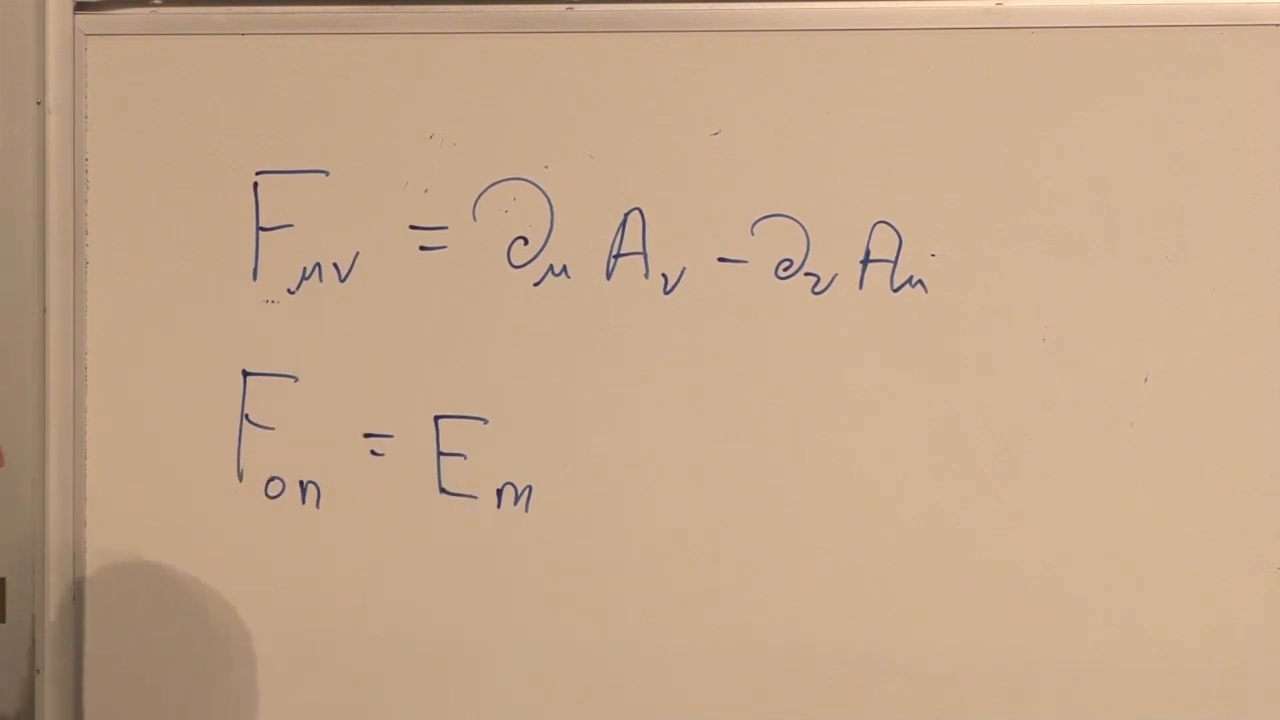
\includegraphics[width=\linewidth]{lecture_08_figure_02.png}\caption{장 텐서의 정의와 전기장으로 식별되는 시간--공간 혼합 성분.}\par\smallskip
\textit{강의 화면: 00:13:15.}\end{figure}

자기장과의 관계는 같은 정의의 공간 부분이다. 예를 들어
\begin{equation}
B_x
=
\partial_yA_z-\partial_zA_y
=
F_{yz},
\end{equation}
나머지 두 성분은 순환 치환으로 얻는다.

\begin{figure}[H]\centering
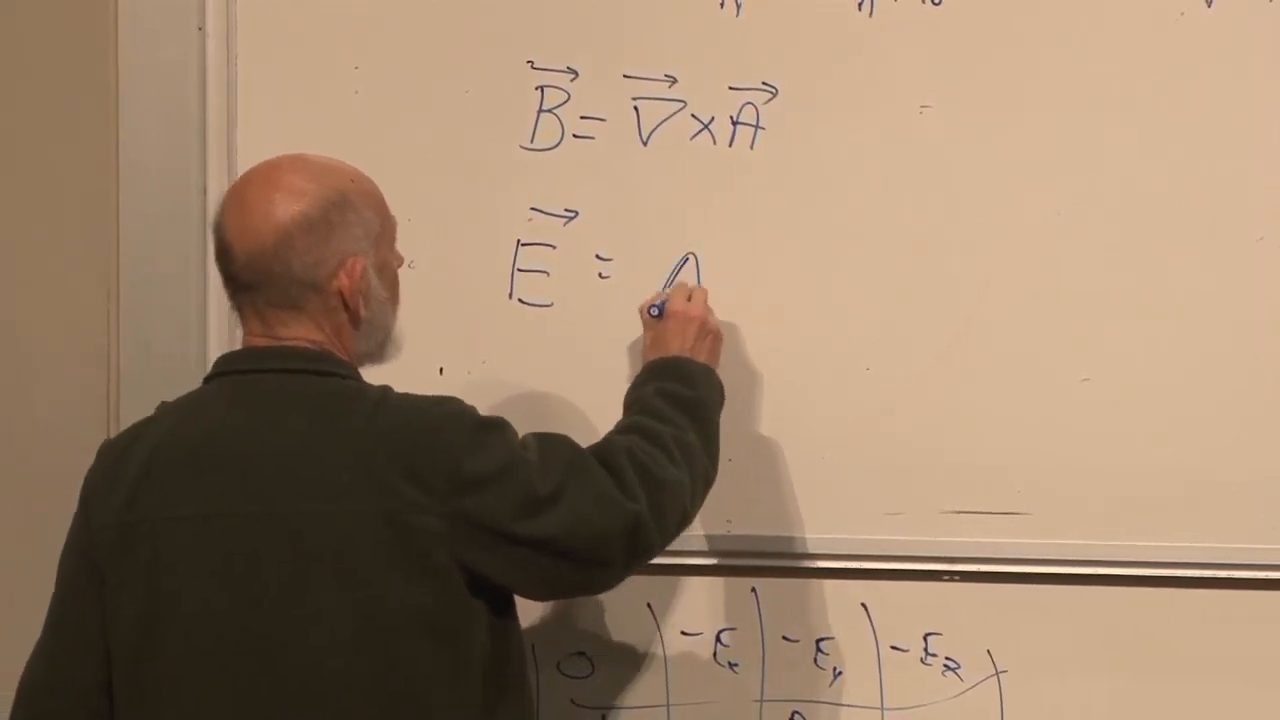
\includegraphics[width=\linewidth]{lecture_08_figure_03.png}\caption{칠판에 모아 쓴 전기장의 벡터 퍼텐셜 식과 자기장의 회전.}\par\smallskip
\textit{강의 화면: 00:14:00.}\end{figure}

\subsection{성분 배열}

첫 번째 텐서 첨자를 행, 두 번째 첨자를 열의 표지로 삼고, 순서는 \(0,x,y,z\)로 하자. 그러면
\begin{equation}
F_{\mu\nu}
=
\begin{pmatrix}
0&E_x&E_y&E_z\\
-E_x&0&B_z&-B_y\\
-E_y&-B_z&0&B_x\\
-E_z&B_y&-B_x&0
\end{pmatrix}.
\label{eq:f-lower-matrix}
\end{equation}
시간--공간 혼합 성분에는 \(\mathbf E\)가 들어 있고, 공간 \(3\times3\) 블록에는 \(\mathbf B\)가 들어 있다. 아래쪽 삼각 영역은 위쪽 삼각 영역을 반사해 부호를 바꾼 것뿐이므로 새로운 정보가 아니다.

\begin{figure}[H]\centering
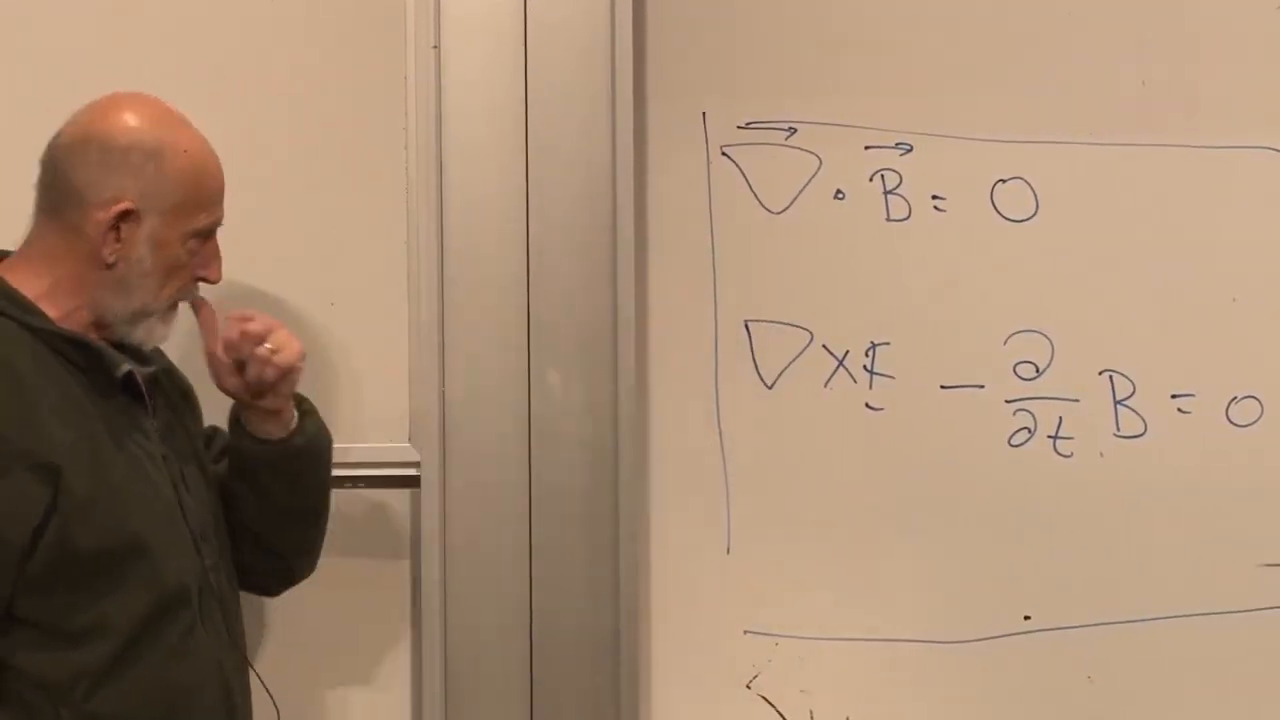
\includegraphics[width=\linewidth]{lecture_08_figure_04.png}\caption{전기 성분과 자기 공간 블록을 갖춘 아래 첨자 전자기장 텐서.}\par\smallskip
\textit{강의 화면: 00:17:15.}\end{figure}

두 첨자를 모두 올리면 모든 전기 성분의 부호가 바뀌고 자기 성분은 그대로다.
\begin{equation}
F^{\mu\nu}
=
\begin{pmatrix}
0&-E_x&-E_y&-E_z\\
E_x&0&B_z&-B_y\\
E_y&-B_z&0&B_x\\
E_z&B_y&-B_x&0
\end{pmatrix}.
\label{eq:f-upper-matrix}
\end{equation}
전기 성분에는 시간 첨자가 하나 있으므로 부호가 한 번 바뀐다. 자기 성분에는 공간 첨자가 두 개 있으므로 부호가 바뀌지 않는다.

\begin{classroomqa}\audiencequestion{행렬을 제대로 읽었다면 자기 성분에는 시간 첨자가 없는 건가요?}\lecturerresponse{그렇다. 자기 성분은 순수한 공간 블록에 놓인다. 전기 성분은 첫째 행과 첫째 열에 있는 시간--공간 혼합 성분이다. \lecturetimestamp{00:18:55}}\end{classroomqa}

\section{순수 자기장을 부스트하기}

\(x\)방향으로 부스트하고 \(c=1\)이라 하자.
\begin{align}
t'&=\gamma(t-vx),
&
x'&=\gamma(x-vt),
&
y'&=y,
&
z'&=z,
\end{align}
여기서
\begin{equation}
\gamma=\frac{1}{\sqrt{1-v^2}}.
\end{equation}
행렬로 쓰면 다음과 같다.
\begin{equation}
x'^\mu
=
\Lambda^\mu{}_\nu x^\nu,
\qquad
\Lambda^\mu{}_\nu
=
\begin{pmatrix}
\gamma&-\gamma v&0&0\\
-\gamma v&\gamma&0&0\\
0&0&1&0\\
0&0&0&1
\end{pmatrix}.
\label{eq:x-boost}
\end{equation}

\begin{classroomqa}\audiencequestion{부스트 행렬에서 마이너스 부호가 빠진 것 아닌가요?}\lecturerresponse{그렇다. 시간--공간 비대각 성분에는 \(t'=\gamma(t-vx)\)와 \(x'=\gamma(x-vt)\)에 필요한 마이너스 부호가 들어간다. 장을 변환하기 전에 이를 바로잡는다. \lecturetimestamp{00:23:50}}\end{classroomqa}

\begin{figure}[H]\centering
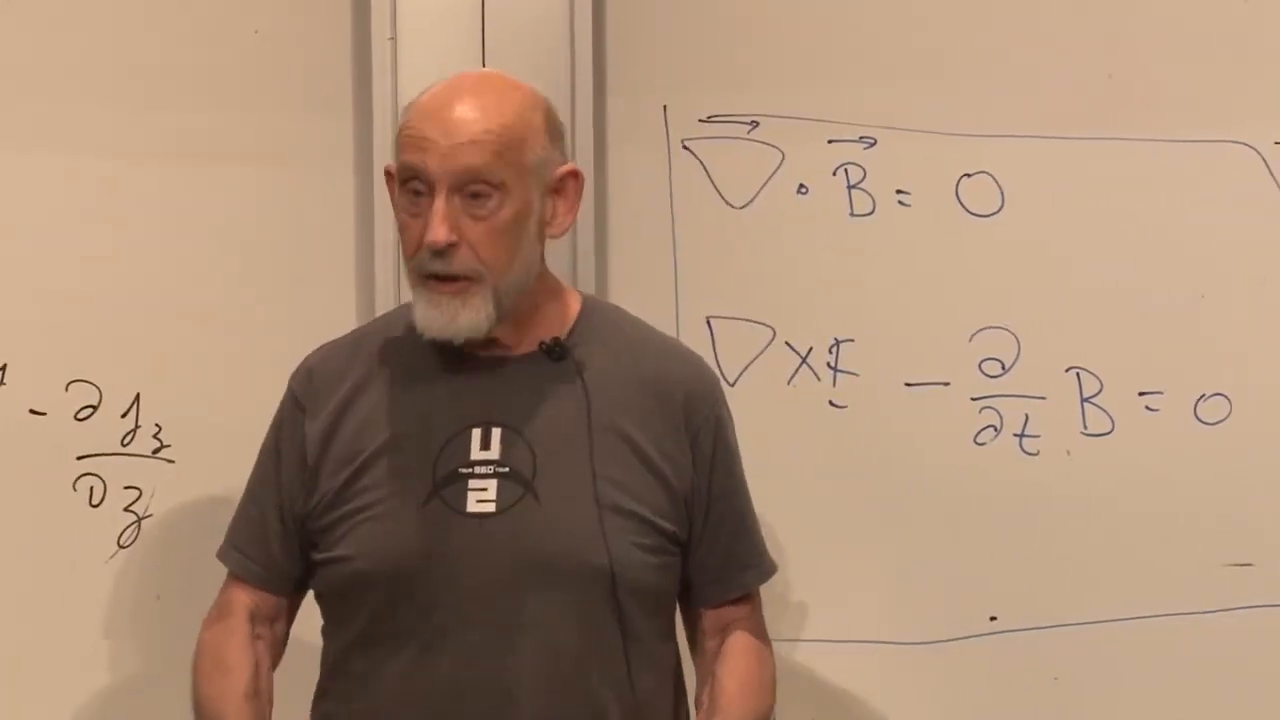
\includegraphics[width=\linewidth]{lecture_08_figure_05.png}\caption{\(x\)축을 따른 운동에 대한 수정된 로런츠 부스트 행렬.}\par\smallskip
\textit{강의 화면: 00:24:00.}\end{figure}

모든 위 첨자 텐서 지수는 위 첨자 벡터 지수처럼 변환한다. 따라서
\begin{equation}
F'^{\mu\nu}
=
\Lambda^\mu{}_\sigma
\Lambda^\nu{}_\tau
F^{\sigma\tau}.
\label{eq:f-boost-law}
\end{equation}
반복된 \(\sigma\)와 \(\tau\)는 더미 지수다. 지수가 더 많은 텐서라면 지수마다 변환 행렬 하나씩이 나타난다.

\begin{figure}[H]\centering
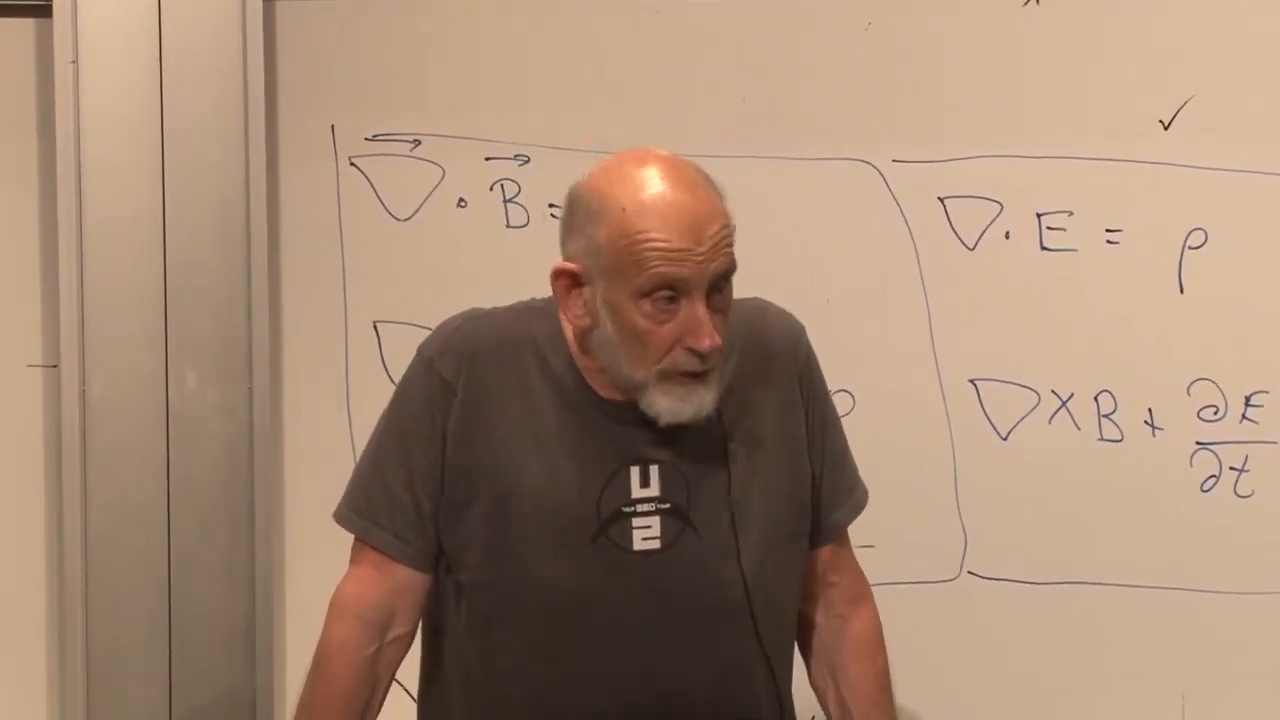
\includegraphics[width=\linewidth]{lecture_08_figure_06.png}\caption{랭크 2 로런츠 변환 법칙. 장 텐서의 각 지수마다 부스트 행렬 하나가 곱해진다.}\par\smallskip
\textit{강의 화면: 00:26:40.}\end{figure}

\subsection{전기장 성분으로 바뀌는 성분}

프라임이 붙지 않은 기준계에 자기장 \(B_y\)만 있다고 하자. ~\eqref{eq:f-upper-matrix}의 규약에 따르면 관련된 독립 성분은
\begin{equation}
F^{xz}=-B_y.
\end{equation}
프라임이 붙은 전기장의 \(z\)성분을 나타내는 혼합 성분 \(F'^{0z}\)을 구하려 한다. \eqref{eq:f-boost-law}에서
\begin{align}
F'^{0z}
&=
\Lambda^0{}_\sigma
\Lambda^z{}_\tau F^{\sigma\tau}
\\
&=
\Lambda^0{}_x\Lambda^z{}_zF^{xz}
\\
&=
(-\gamma v)(1)(-B_y)
=
\gamma vB_y.
\end{align}을 얻는다. 이 규약에서는 \(F'^{0z}=-E'_z\)이므로
\begin{equation}
E'_z=-\gamma vB_y.
\label{eq:boosted-electric-field}
\end{equation}
부호는 정해 둔 축과 장의 규약에 따라 달라진다. 계산에서 변하지 않는 핵심은
\begin{equation}
\lvert E'_z\rvert
=
\gamma\lvert vB_y\rvert
\ne0.
\end{equation}
원래 장에는 독립적인 자기 성분이 하나뿐이므로 이중 합은 이 항 하나만 남는다.

\begin{figure}[H]\centering
\includegraphics[width=\linewidth]{lecture_08_figure_07.png}\caption{부스트 뒤에 선택한 텐서 성분. 원래 자기 성분에 곱해지는 인자는 \(\gamma v\)이다.}\par\smallskip
\textit{강의 화면: 00:32:30.}\end{figure}

프라임이 붙은 기준계가 전하와 함께 움직이도록 하자. 그러면 전하는 정지하므로 전하가 받는 힘에서 자기적 부분 \(q\,\mathbf v'\times\mathbf B'\)은 없다. 그렇다고 힘이 사라지는 것은 아니다. 힘은 \(q\mathbf E'\)이다. 실험실 관찰자가 보는 자기력과 전하와 함께 움직이는 관찰자가 보는 전기력은 동일한 사건에 대한 두 가지 설명이다.

이것이 아인슈타인 논문 첫 문단의 수수께끼에 대한 답이다. 이 질문에 강의에서 대략 처음 40분을 썼다. 역사적으로 보면 아인슈타인은 이 문제를 훨씬 더 오래 붙들고 있었다는 농담도 있다. 전기장과 자기장이 섞인다는 구호를 하나의 명시적인 텐서 성분으로 보여 주므로, 이 계산에 시간을 들일 만하다.

\section{맥스웰 방정식: 항등식과 동역학}

이제 전하에 작용하는 힘에서 장 방정식으로 넘어가자. 다음 강의에서는 작용으로부터 장 방정식을 유도할 것이다. 여기서는 우선 방정식들을 제시하고, 서로 다른 두 가지 논리적 역할을 이해하며, 항등식에 근거한 절반을 공변 형식으로 표현하는 것이 목적이다.

\begin{classroomqa}\audiencequestion{이 방정식들은 이미 유도하지 않았나요?}\lecturerresponse{주어진 전자기장 속에서 대전 입자의 운동 방정식은 유도했다. 맥스웰 방정식은 전하와 전류에 대한 장의 반응을 포함하여 장 자체의 운동 방정식을 나타낸다. \lecturetimestamp{00:35:10}}\end{classroomqa}

\begin{classroomqa}\audiencequestion{맥스웰 방정식은 몇 개인가요?}\lecturerresponse{성분 방정식으로는 스칼라 방정식이 8개다. 벡터 표기법에서는 이를 스칼라 방정식 2개와 3성분 벡터 방정식 2개로 묶어, 관례적으로 맥스웰 방정식 4개라고 부른다. \lecturetimestamp{00:35:24}}\end{classroomqa}

\(c=1\)이고 통상적인 진공 상수들이 전하와 전류의 정의에 흡수된 단위를 계속 사용한다. 8개 성분 방정식 가운데 4개는 정의 \(F=dA\)에서 따른다. 이들은 운동학적 항등식이다. 나머지 4개는 동역학적 방정식이며, 장의 작용이 달라지면 함께 달라질 수 있다.

\subsection{기본 벡터 연산 세 가지}

미분 가능한 3차원 벡터장 \(\mathbf A\)에 대해
\begin{align}
(\boldsymbol\nabla\times\mathbf A)_x
&=
\partial_yA_z-\partial_zA_y,
\\
\boldsymbol\nabla\cdot\mathbf A
&=
\partial_xA_x+\partial_yA_y+\partial_zA_z.
\end{align}
나머지 회전 성분은 \(x\to y\to z\to x\)를 순환 치환해 얻는다. 스칼라장 \(s\)에 대해서는
\begin{equation}
\boldsymbol\nabla s
=
(\partial_xs,\partial_ys,\partial_zs).
\end{equation}
따라서 회전은 벡터이고, 발산은 스칼라이며, 기울기는 벡터다.

\begin{classroomqa}\audiencequestion{회전과 발산의 정의를 처음부터 전부 복습할 필요가 있나요?}\lecturerresponse{성분별 정의는 적어 두었지만 나머지 성분을 모두 전개할 필요는 없다. 좌표 표지를 순환시키면 얻을 수 있다. \lecturetimestamp{00:37:32}}\end{classroomqa}

매끄러운 함수의 편미분은 교환 가능하므로 다음 두 항등식이 성립한다.
\begin{align}
\boldsymbol\nabla\cdot
(\boldsymbol\nabla\times\mathbf A)
&=0,
\label{eq:div-curl}
\\
\boldsymbol\nabla\times
(\boldsymbol\nabla s)
&=\mathbf0.
\label{eq:curl-grad}
\end{align}

\begin{classroomqa}
\audiencequestion{컬의 발산이 사라짐을 보이는 성분별 증명을 전부 써 볼까요?}
\lecturerresponse{수강생들은 쓰지 않기로 한다. 성분을 전개하면 \(\partial_x\partial_yA_z\)와 \(-\partial_y\partial_xA_z\) 같은 항들이 쌍으로 나타나며, 미분 순서를 바꿀 수 있으므로 서로 상쇄된다. \lecturetimestamp{00:40:13}}
\end{classroomqa}

\begin{figure}[H]\centering
\includegraphics[width=\linewidth]{lecture_08_figure_08.png}\caption{맥스웰 방정식의 절반을 얻는 데 쓰인 회전의 발산과 기울기의 회전 항등식.}\par\smallskip
\textit{강의 화면: 00:41:40.}\end{figure}

\subsection{벡터 퍼텐셜에서는 자기 원천이 생기지 않는다}

~\eqref{eq:b-from-a}의 발산을 취하면
\begin{equation}
\boldsymbol\nabla\cdot\mathbf B
=
\boldsymbol\nabla\cdot
(\boldsymbol\nabla\times\mathbf A)
=0.
\label{eq:div-b-zero}
\end{equation}
운동 방정식은 사용하지 않았다. 이 결과는 퍼텐셜 표현과 매끄러운 편미분만으로 따른다.

\begin{figure}[H]\centering
\includegraphics[width=\linewidth]{lecture_08_figure_09.png}\caption{자기장의 발산이 회전의 발산으로 환원된다.}\par\smallskip
\textit{강의 화면: 00:43:05.}\end{figure}

\begin{classroomqa}\audiencequestion{전기장의 발산은 무엇인가요?}\lecturerresponse{사용하는 단위계에서는 전하 밀도, 즉 \(\boldsymbol\nabla\cdot\mathbf E=\rho\)이다. 점전하는 전기력선이 원천에서 퍼져 나가는 대표적인 예다. \lecturetimestamp{00:43:20}}\end{classroomqa}

기초적인 수준에서 보면 ~\eqref{eq:div-b-zero}은 자기 전하 밀도가 없다는 뜻이다. 매끄럽고 전역적으로 정의된 벡터 퍼텐셜로는 자기 단극자 원천을 만들 수 없다. 다만 이 진술에는 나중에 조건을 덧붙여야 한다. 겹치는 패치에서 정의된 퍼텐셜이나 특이한 게이지 선택을 사용하면 자기 단극자를 기술할 수 있다. 강의에서는 이 정교한 논의를 뒤로 미룬다.

\subsection{전기 퍼텐셜에서 얻는 패러데이 방정식}

식~\eqref{eq:e-from-a}을 삼차원 벡터 표기로 쓰면 다음과 같다.
\begin{equation}
\mathbf E
=
\frac{\partial\mathbf A}{\partial t}
-\boldsymbol\nabla A_0.
\label{eq:e-vector-potential}
\end{equation}
\(A_0\)는 사차원 벡터의 성분이지만, 통상적인 공간 회전에서는 스칼라이다. 컬을 취하면 다음과 같다.
\begin{align}
\boldsymbol\nabla\times\mathbf E
&=
\boldsymbol\nabla\times
\frac{\partial\mathbf A}{\partial t}
-
\boldsymbol\nabla\times
(\boldsymbol\nabla A_0)
\\
&=
\frac{\partial}{\partial t}
(\boldsymbol\nabla\times\mathbf A)
\\
&=
\frac{\partial\mathbf B}{\partial t}.
\end{align}
공간 컬은 시간 미분과 교환되며, 기울기의 컬은 사라진다.

\begin{figure}[H]\centering
\includegraphics[width=\linewidth]{lecture_08_figure_10.png}\caption{자기장의 회전과 전기 퍼텐셜 식, 그리고 회전 계산의 시작을 함께 적은 칠판 모습.}\par\smallskip
\textit{강의 화면: 00:47:45.}\end{figure}

따라서 비동차항이 없는 성분 방정식 4개는 다음과 같다.
\begin{align}
\boldsymbol\nabla\cdot\mathbf B&=0,
\label{eq:homogeneous-div}
\\
\boldsymbol\nabla\times\mathbf E
-\frac{\partial\mathbf B}{\partial t}
&=\mathbf0.
\label{eq:homogeneous-curl}
\end{align}
첫째는 스칼라 방정식 하나이고, 둘째는 3성분 벡터 방정식이다.

\begin{figure}[H]\centering
\includegraphics[width=\linewidth]{lecture_08_figure_11.png}\caption{퍼텐셜의 정의에서 직접 얻은 원천이 없는 맥스웰 방정식 쌍.}\par\smallskip
\textit{강의 화면: 00:48:45.}\end{figure}

\subsection{동역학에 해당하는 절반}

나머지 방정식은 다음과 같다.
\begin{align}
\boldsymbol\nabla\cdot\mathbf E&=\rho,
\label{eq:gauss-electric}
\\
\boldsymbol\nabla\times\mathbf B
+\frac{\partial\mathbf E}{\partial t}
&=-\mathbf J.
\label{eq:ampere-maxwell}
\end{align}
이 방정식들은 \(F=dA\)에서 따르지 않는다. 원천이 어떻게 장을 만들고 변화시키는지를 기술하며, 다음 강의에서 전자기 작용으로부터 유도할 것이다. 전류 항의 마이너스 부호는 이미 정한 규약으로 결정된다. 즉 \(F_{0i}=E_i\), \(F_{ij}=\epsilon_{ijk}B_k\), 그리고 \(\partial_\mu F^{\mu\nu}=J^\nu\)이다. 강의 중 칠판에는 처음에 \(\mathbf J\)가 이 마이너스 부호 없이 우변에 적혔다. 그 결과 전하 보존 법칙과 맞지 않는 점을 다음 강의에서 알아차리고 바로잡는다.

\begin{classroomqa}\audiencequestion{회전 방정식 우변에는 어떤 종류의 물리량이 있나요?}\lecturerresponse{좌변이 3차원 벡터이므로 우변도 3차원 벡터이며, 이를 전류 밀도 \(\mathbf J\)라고 한다. 가우스 방정식 우변은 3차원 스칼라 전하 밀도 \(\rho\)다. \lecturetimestamp{00:50:36}}\end{classroomqa}

\begin{figure}[H]\centering
\includegraphics[width=\linewidth]{lecture_08_figure_12.png}\caption{항등식에 근거한 쌍과 원천이 있는 동역학적 쌍으로 묶어 쓴 맥스웰 방정식 4개.}\par\smallskip
\textit{강의 화면: 00:50:40.}\end{figure}

\section{시공간의 흐름으로서의 전하와 전류}

이제 기호 \(\rho\)와 \(\mathbf J\)에 기하학적 의미를 부여해야 한다. 전하 밀도는 단위 부피당 전하이고, 전류 밀도는 단위 시간 동안 방향이 정해진 면을 통과하는 전하량이다. 강의에서는 두 양을 모두 세계선에서 출발해 설명한다. 그래야 나중에 이들이 하나의 4-벡터로 합쳐지는 일이 우연처럼 보이지 않을 것이다.

\subsection{옆 칠판에 보이는 내용에 관한 수업 중 여담}

세계선을 그리기 전에 옆 강의실에 보이는 방정식들 때문에 잠시 수업에서 벗어나 이야기를 나눈다. 곧 개설될 강좌에서는 양자장론과 현대 수학과의 관련성을 이해하는 데 필요한 배경을 얻고 싶어 하는 수학 교수진에게 양자역학을 소개할 예정이었다. 어려움은 양쪽 모두에 있다. 물리학자는 암묵적으로 익힌 물리학적 사고방식을 명시적으로 설명해야 하고, 수학자는 형식적 구조가 무엇을 기술하도록 고안되었는지 배워야 한다.

\begin{classroomqa}\audiencequestion{그 강의는 누가 힘들어할까요?}\lecturerresponse{아마 양쪽 모두일 것이다. 익숙하지 않은 청중을 가르치는 물리학자와, 형식론의 바탕이 되는 물리학적 사고방식에 부딪히는 수학자 모두 그렇다. 그래도 그 강의는 재미있을 것으로 예상된다. 이어서 수업은 전하와 전류로 돌아간다. \lecturetimestamp{00:53:20}}\end{classroomqa}

\subsection{전하 밀도}

시간을 세로축으로 그리고, 나머지 축은 3차원 공간을 나타내도록 하자. 대전 입자들은 세계선을 그린다. 한 시각을 고정하고 부피가 \(\Delta V\)인 작은 공간 정육면체를 그 세계선 다발에 걸쳐 놓은 뒤, 그 안에 있는 입자들의 전하를 모두 더한다. 전하 밀도는
\begin{equation}
\rho(t,\mathbf x)
=
\lim_{\Delta V\to0}
\frac{\Delta Q}{\Delta V}.
\label{eq:charge-density}
\end{equation}
칠판에 그린 2차원 정사각형은 3차원 정육면체를 나타낸다. 네 차원을 평면 칠판에 그릴 수 없어 공간 방향 하나를 생략했을 뿐이다.

\begin{figure}[H]\centering
\includegraphics[width=\linewidth]{lecture_08_figure_13.png}\caption{작은 공간 셀을 통과하는 대전 입자들의 세계선. \(\rho=\Delta Q/\Delta V\).}\par\smallskip
\textit{강의 화면: 00:57:20.}\end{figure}

\subsection{전류 밀도}

시공간 셀을 옆으로 돌려 보자. \(J_x\)를 정의하려면 \(yz\)면 안에 놓인 작은 창의 넓이 \(\Delta A_x\)를 택한다. 이 창은 \(x\)축에 수직이다. \(\Delta t\) 동안 음의 \(x\) 쪽에서 양의 \(x\) 쪽으로 통과하는 순전하량을 센다.
\begin{equation}
J_x
=
\lim_{\Delta A_x,\Delta t\to0}
\frac{\Delta Q_x}{\Delta A_x\,\Delta t}.
\label{eq:jx-window}
\end{equation}
방향이 부호를 정한다. \(y\)와 \(z\)에 수직인 창으로도 같은 방식으로 \(J_y\)와 \(J_z\)을 정의한다.

칠판 그림은 그리기 어려운 점을 그대로 드러낸다. \(yz\)면에 놓인 창은 벽의 창보다 천장에 난 창처럼 보인다. 한 번에 표시할 수 있는 축보다 관련된 축이 더 많기 때문이다. 스케치는 명확하지 않아도 불변인 정의 자체는 모호하지 않다.

\begin{classroomqa}\audiencequestion{그림에서 창은 천장에 나 있는 건가요?}\lecturerresponse{방에 비유하자면 그렇다. 중요한 것은 창의 면이 \(x\) 방향에 수직이라는 점이다. 넓이가 \(yz\)인 면은 그 면을 통과하는 \(x\) 방향 전류를 잰다. \lecturetimestamp{00:59:38}}\end{classroomqa}

\begin{figure}[H]\centering
\includegraphics[width=\linewidth]{lecture_08_figure_14.png}\caption{횡방향 창을 통과하는 전하 전류. \(J_x=\Delta Q/(\Delta A\,\Delta t)\).}\par\smallskip
\textit{강의 화면: 01:01:40.}\end{figure}

\begin{figure}[H]\centering
\includegraphics[width=\linewidth]{lecture_08_figure_15.png}\caption{세 공간축에 수직인 창을 통과하는 전하량으로 정의한 전류의 세 성분.}\par\smallskip
\textit{강의 화면: 01:02:40.}\end{figure}

네 물리량은 서로 짝을 이루는 방식으로 정의된다. 한순간의 공간 부피는 시간축에 수직인 초곡면이므로, \(\rho\)은 시간축에 수직인 창을 통과하는 전하 흐름이다. \(J_i\)는 공간축에 수직인 창들을 통과하는 흐름이다.

\begin{classroomqa}\audiencequestion{네 성분은 시간 방향의 흐름 하나와 공간 방향의 흐름 세 개인가요?}\lecturerresponse{그렇게 생각하면 정확하다. 공간 부피는 시간축에 수직인 창이고, 세 횡방향 면은 각각 \(x\), \(y\), \(z\)에 수직인 창이다. 이 네 가지 플럭스는 함께 묶인다. \lecturetimestamp{01:04:14}}\end{classroomqa}

이로부터 반변 4-전류를 생각할 수 있다.
\begin{equation}
J^\mu
=
(\rho,J_x,J_y,J_z).
\label{eq:four-current}
\end{equation}

\begin{classroomqa}\audiencequestion{계량은 어디에 들어가나요? 이 전류는 공변인가요, 반변인가요?}\lecturerresponse{여기서 정의한 \(\rho\)과 세 \(J_i\)는 \(J^\mu\)의 성분이며, 위 첨자를 가진 반변 4-벡터를 이룬다. \(J_\mu\)가 필요하면 계량을 이용해 지수를 내린다. 공변적인 맥스웰 방정식의 표현을 보면 위 첨자를 택한 것이 왜 자연스러운지 알 수 있다. \lecturetimestamp{01:04:48}}\end{classroomqa}

\section{휴식 시간의 막간: 블랙홀 근처의 신호}

예정된 휴식 시간에 질문은 앞서 나눈 블랙홀 이야기로 이어진다. 전기역학에서 벗어난 여담이지만, 수업 중 상당한 토론이 오갔고 서로 다른 관찰자의 설명을 구분하는 같은 사고방식을 보여 준다.

\begin{classroomqa}\audiencequestion{멀리 떨어진 관찰자에게 낙하하는 물체가 사건의 지평선 근처에서 느려지는 것으로 보인다면, 블랙홀은 과거에 낙하한 모든 물체로 덮여 보이나요?}\lecturerresponse{슈바르츠실트 좌표 시간으로 기술하면 고전적인 낙하 물체는 점근적으로 사건의 지평선에 접근하는 것으로 보인다. 물질이 차례로 쌓여 지평선 근처의 층이 점점 압축되는 모습을 그려 볼 수 있다. 하지만 관측 가능한 실제 신호는 점점 더 지연되고 적색편이되며 희미해진다. 보통의 국소 진동수로 방출된 빛은 처음에는 가시광선으로 도착하고, 이어 적외선, 마이크로파, 전파로 도착하며, 광자 하나하나의 에너지도 줄어든다. 현실적인 원거리 검출기라면 얼어붙은 듯한 밝은 물체를 영원히 보지는 못한다. 그것은 희미해져 어둠 속으로 사라진다.
\lecturetimestamp{01:06:11}}\end{classroomqa}

낙하하는 관찰자의 시계와 그 관찰자가 국소적으로 켠 손전등은 그 관찰자에게 평범하게 보인다. 원거리 관찰자의 설명이 달라지는 것은 진동수와 도착률이 적색편이되기 때문이다. 에너지와 대역폭이 유한하므로, 메시지 중 마지막으로 분해해 볼 수 있는 부분이 사실상 존재한다.

\begin{classroomqa}\audiencequestion{물체가 점근적으로 사건의 지평선에 접근하는 건가요?}\lecturerresponse{원거리 관찰자의 슈바르츠실트 좌표 설명에서는 그렇다. 양자역학적으로는 희미해지는 신호를 블랙홀의 호킹 복사와도 구별해야 한다. 충분히 늦은 시각에는 약하게 적색편이된 신호가 블랙홀 자체에서 나오는 복사의 배경에 묻혀 관측되지 않게 된다. \lecturetimestamp{01:09:24}}\end{classroomqa}

\begin{classroomqa}\audiencequestion{적색편이된 파장이 관측 가능한 우주의 크기를 넘어 커지면 어떻게 되나요?}\lecturerresponse{실제로는 그 한계에 도달하기 훨씬 전에 신호를 잃어버린다. 강의에서는 대략적인 호킹 복사 그림으로, 빛이 블랙홀을 가로지르는 시간마다 전형적인 양자 하나 정도가 방출된다고 설명한다.
\[
t_{\rm cross}\sim\frac{R_s}{c}.
\]
큰 블랙홀의 복사는 극도로 약하다. 적색편이된 낙하 신호는 우주론적 파장 한계에 이르기 훨씬 전에 검출 불가능해진다. \lecturetimestamp{01:09:50}}\end{classroomqa}

\begin{classroomqa}\audiencequestion{블랙홀의 수명 내내 통과 시간당 양자 하나 정도라는 방출률이 일정한가요?}\lecturerresponse{아니다. 증발하는 슈바르츠실트 블랙홀은 크기가 줄어들므로 통과 시간은 짧아지고 호킹 온도는 올라간다. 따라서 방출은 점점 빨라진다. 순간적인 반지름으로 나타낸 차원 추정은 여전히 유용하지만, 반지름은 일정하지 않다. 이에 따라 전형적인 호킹 파장은 증발이 진행될수록 짧아진다. \lecturetimestamp{01:11:42}}\end{classroomqa}

휴식 시간이 끝나고 재킷을 벗은 뒤, \(\rho\)와 \(\mathbf J\)로 돌아간다.

\section{전하의 국소 보존}

전하 보존을 다음과 같이만 말하고 싶은 유혹이 있다.
\begin{equation}
\frac{dQ_{\rm universe}}{dt}=0.
\end{equation}
하지만 이 진술은 너무 약하다. 전체 전하가 변하지 않은 채 실험실에서 사라진 전하가 즉시 알파 센타우리로, 혹은 더 멀리 떨어진 머리털자리 은하단으로 다시 나타날 수도 있기 때문이다. 그런 법칙은 실험적으로 검증할 여지가 거의 없다.

더 강한 진술은 국소적이다. 어떤 영역 안의 전하가 변할 수 있는 것은 그 영역의 경계를 통과할 때뿐이다. 한 점을 둘러싸는 작은 상자를 놓자. 상자 안의 전하가 증가하면 여섯 면을 통과하는 순전류가 안쪽을 향해야 한다. 전하가 감소하면 순전류는 바깥쪽을 향해야 한다.

\subsection{마주 보는 면을 통과하는 플럭스}

\(x\)에 수직인 두 면을 보자. 한 면의 안쪽 방향 기여는 \(x\)의 한 값에서 계산하고, 반대쪽 면의 기여는 그로부터 작은 거리만큼 떨어진 곳에서 계산한다. 두 기여의 차이를 상자 폭으로 나눈 값은 다음에 가까워진다.
\begin{equation}
-\partial_xJ_x.
\end{equation}
양의 \(J_x\)를 \(x\)가 증가하는 방향으로 흐르는 것으로 정의했지만 바깥쪽 플럭스는 상자 안의 전하를 감소시키므로 마이너스 부호가 붙는다. \(y\)면과 \(z\)면의 쌍도 마찬가지로 각각 \(-\partial_yJ_y\)와 \(-\partial_zJ_z\)를 기여한다. 따라서
\begin{equation}
\frac{\partial\rho}{\partial t}
=
-\partial_xJ_x-\partial_yJ_y-\partial_zJ_z
=
-\boldsymbol\nabla\cdot\mathbf J.
\end{equation}
동등하게,
\begin{equation}
\boxed{
\frac{\partial\rho}{\partial t}
+\boldsymbol\nabla\cdot\mathbf J=0
}.
\label{eq:continuity}
\end{equation}

\begin{figure}[H]\centering
\includegraphics[width=\linewidth]{lecture_08_figure_16.png}\caption{국소 보존 법칙 \(\dot\rho=-\boldsymbol\nabla\cdot\mathbf J\)과, 경계면의 전류를 통해 그 법칙이 나타나는 작은 상자.}\par\smallskip
\textit{강의 화면: 01:20:45.}\end{figure}

통상 이 식을 연속 방정식이라고 부른다. 강의에서는 \emph{국소 보존}이라는 이름을 선호한다. 연속이라는 말은 수학적 매끄러움 조건을 떠올리게 할 수 있지만, 물리적 내용은 전류가 그 사이를 흐르지 않는 한 전하가 여기서 사라졌다가 저기서 다시 나타날 수 없다는 것이다.

\subsection{맥스웰이 변위 전류를 도입해야 했던 이유}

식~\eqref{eq:continuity}은 맥스웰 방정식에 독립적으로 추가되는 식이 아니다. 가우스 법칙을 시간에 대해 미분하고 앙페르--맥스웰 법칙의 발산을 취하면 다음과 같다.
\begin{align}
\frac{\partial\rho}{\partial t}
&=
\boldsymbol\nabla\cdot
\frac{\partial\mathbf E}{\partial t},
\\
-\boldsymbol\nabla\cdot\mathbf J
&=
\boldsymbol\nabla\cdot
(\boldsymbol\nabla\times\mathbf B)
+
\boldsymbol\nabla\cdot
\frac{\partial\mathbf E}{\partial t}
\\
&=
\boldsymbol\nabla\cdot
\frac{\partial\mathbf E}{\partial t}.
\end{align}
따라서 두 좌변은 같으며, 이에 따라 \(\partial_t\rho=-\boldsymbol\nabla\cdot\mathbf J\)가 되고, 이는 정확히 식~\eqref{eq:continuity}이다. 구조적으로 중요한 점은 전하 보존과 발산 관계가 서로 양립하려면 \(\mathbf E\), 즉 변위 전류 항의 시간 미분이 꼭 필요하다는 것이다.

\begin{classroomqa}
\audiencequestion{전하를 포함하는 두 맥스웰 방정식이 어디서 나오는지는 아직 보이지 않았죠?}
\lecturerresponse{그렇다. 이 방정식들은 다음에 작용으로부터 유도할 동역학적 목표다. 정자기 컬 법칙은 맥스웰 이전부터 알려져 있었고, 맥스웰의 결정적인 시간 의존성 추가 항은 변위 전류였다. 이 항이 있어야 장 방정식이 국소 전하 보존과 양립한다. \lecturetimestamp{01:23:15}}
\end{classroomqa}

발산을 상세히 계산하는 과정은 강의에서 연습문제로 남겨 두지만, 그 결론은 선택 사항이 아니다. 맥스웰 방정식은 전하 보존을 요구한다.

\section{4-전류와 그 발산}

식~\eqref{eq:continuity}을 성분별로 쓰면 다음과 같다.
\begin{equation}
\frac{\partial\rho}{\partial t}
+
\frac{\partial J_x}{\partial x}
+
\frac{\partial J_y}{\partial y}
+
\frac{\partial J_z}{\partial z}
=0.
\label{eq:continuity-components}
\end{equation}

\begin{figure}[H]
\centering
\includegraphics[width=\linewidth]{lecture_08_figure_17.png}
\caption{국소 전하 보존을 시간 미분 하나와 공간 미분 세 개로 전개한 식.}
\par\smallskip
\textit{강의 시각: 01:25:40.}
\end{figure}

\(J^\mu\)를 식~\eqref{eq:four-current}으로 정의하면, 네 항은 하나의 수축으로 표현된다.
\begin{equation}
\boxed{\partial_\mu J^\mu=0}.
\label{eq:four-current-conservation}
\end{equation}
\(\partial_\mu\)의 아래 첨자는 \(J^\mu\)의 위 첨자와 수축하므로, 그 결과는 로런츠 스칼라이다. 기하학적 창 구성은 이미 이러한 변환 법칙을 시사했다. \(\rho\)와 전류의 세 성분은 같은 전하 흐름을 네 방향에서 본 것이다.

\begin{figure}[H]
\centering
\includegraphics[width=\linewidth]{lecture_08_figure_18.png}
\caption{성분 \((\rho,J_x,J_y,J_z)\)을 \(J^\mu\)로 모아 4-기울기와 수축한다.}
\par\smallskip
\textit{강의 시각: 01:27:10.}
\end{figure}

\begin{classroomqa}
\audiencequestion{\(\rho\)의 시간 미분은 언제 편미분이 되었나요?}
\lecturerresponse{처음부터 편미분이었다. 우리는 공간 상자를 고정해 두고 시간에 따라 그 안의 전하 밀도가 어떻게 변하는지 묻는다. 움직이는 궤적을 따라가는 것이 아니므로, 여기서 \(\dot\rho\)는 고정된 \(x,y,z\)에서의 \(\partial\rho/\partial t\)를 뜻한다.
\lecturetimestamp{01:28:20}}
\end{classroomqa}

\section{공변 형식으로 쓴 동차 방정식}

이제 필요한 대상들이 갖추어졌다.
\begin{itemize}
\item \(\mathbf E\)와 \(\mathbf B\)는 반대칭 텐서 \(F_{\mu\nu}\)의 서로 독립인 여섯 성분이고,
\item \(\rho\)와 \(\mathbf J\)는 \(J^\mu\)의 네 성분이며,
\item 국소 보존은 스칼라 방정식 \(\partial_\mu J^\mu=0\)이다.
\end{itemize}
이번 강의에서 남은 과제는 동차 맥스웰 방정식 쌍, 즉 식~\eqref{eq:homogeneous-div}과 식\eqref{eq:homogeneous-curl}을 하나의 텐서 방정식으로 쓰는 것이다.

\subsection{순환 미분}

답은 다음과 같다.
\begin{equation}
\boxed{
\partial_\sigma F_{\nu\tau}
+
\partial_\nu F_{\tau\sigma}
+
\partial_\tau F_{\sigma\nu}
=0
}.
\label{eq:bianchi}
\end{equation}
세 항에서는 미분 지수와 장 텐서의 두 지수가 순환적으로 자리를 바꾼다. 이를 흔히 다음과 같이 줄여 쓴다.
\begin{equation}
\partial_{[\sigma}F_{\nu\tau]}=0,
\end{equation}
여기서 대괄호는 반대칭화를 뜻한다.

\begin{figure}[H]
\centering
\includegraphics[width=\linewidth]{lecture_08_figure_19.png}
\caption{동차 맥스웰 방정식들을 하나로 묶어 나타내는 순환형 세 지표 방정식.}
\par\smallskip
\textit{강의 시점: 01:33:20.}
\end{figure}

\subsection{세 지수가 모두 공간 지수인 경우}

다음과 같이 두자.
\begin{equation}
(\sigma,\nu,\tau)=(x,y,z).
\end{equation}
그러면 다음과 같다.
\begin{align}
0
&=
\partial_xF_{yz}
+
\partial_yF_{zx}
+
\partial_zF_{xy}
\\
&=
\partial_xB_x+\partial_yB_y+\partial_zB_z
\\
&=
\boldsymbol\nabla\cdot\mathbf B.
\end{align}
따라서 식~\eqref{eq:bianchi}에서 세 지수가 모두 공간 지수인 성분은 자기장의 발산이 없다는 조건과 정확히 일치한다.

\begin{figure}[H]
\centering
\includegraphics[width=\linewidth]{lecture_08_figure_20.png}
\caption{순환 항등식에서 모든 지표가 공간 지표인 성분을 \(\partial_xB_x+\partial_yB_y+\partial_zB_z=0\)로 줄인 식.}
\par\smallskip
\textit{강의 시점: 01:35:30.}
\end{figure}

\subsection{시간 지수 하나}

예를 들어 다음을 택하자.
\begin{equation}
(\sigma,\nu,\tau)=(y,x,0).
\end{equation}
그러면 식~\eqref{eq:bianchi}은 전기장 성분의 공간 미분 두 개와 자기장 성분의 시간 미분 하나를 결합한다.
\begin{equation}
\partial_yF_{x0}
+
\partial_xF_{0y}
+
\partial_0F_{yx}
=0.
\end{equation}
식~\eqref{eq:f-lower-matrix}의 행렬을 이용하면 이는 다음 방정식의 한 성분이다.
\begin{equation}
\boldsymbol\nabla\times\mathbf E
-\frac{\partial\mathbf B}{\partial t}
=\mathbf0,
\end{equation}
상대 부호는 반대칭성에 의해 정해진다. 공간 지수의 다른 조합을 택하면 컬 방정식의 나머지 두 성분을 얻는다.

\begin{figure}[H]
\centering
\includegraphics[width=\linewidth]{lecture_08_figure_21.png}
\caption{파라데이 방정식의 한 성분을 얻는 시간 지표 하나와 공간 지표 둘의 성분 확인.}
\par\smallskip
\textit{강의 시점: 01:38:20.}
\end{figure}

직접 증명할 수도 있다. 식~\eqref{eq:field-tensor-definition}을 식~\eqref{eq:bianchi}에 대입하면 2계 미분 항 여섯 개가 나타나며, 편미분끼리 교환되므로 쌍을 이루어 상쇄된다. 이는 발산의 컬과 기울기의 컬에 관한 항등식을 4차원으로 확장한 것이다.

\begin{classroomqa}
\audiencequestion{비앙키라는 이름에 \(h\)가 들어가나요?}
\lecturerresponse{그렇다. 이 순환 방정식은 전자기 비앙키 항등식이며, 일반 상대성이론에도 나타나는 기하학적 항등식의 특수한 경우다. 더 깊은 기하학적 해석은 뒤로 미룬다.
\lecturetimestamp{01:40:28}}
\end{classroomqa}

\subsection{쓰인 성분은 64개인데 방정식은 네 개뿐인 이유}

각각 네 가지 값을 가질 수 있는 세 지표는 \(4^3=64\)개의 방정식을 만드는 듯하다. 반대칭성으로 중복을 제거하면 다음과 같다.
\begin{itemize}
\item 두 지표가 같으면 순환식은 항등적으로 사라진다.
\item 세 지표가 모두 서로 다르면, 순열에 따라 부호만 달라질 뿐 같은 방정식이 나온다.
\item 사차원에는 서로 다른 지표 세 개로 이루어진 순서 없는 조합이 \(\binom{4}{3}=4\)개뿐이다.
\end{itemize}
모든 지표가 서로 다른 순서 있는 세 지표의 배열은 \(24\)개이며, 이는 각각 여섯 순열로 이루어진 네 묶음으로 나뉜다. 나머지 \(40\)개의 배열은 사라진다. 서로 독립인 네 방정식은 자기장 발산 방정식 하나와 패러데이 방정식의 세 성분이다.

\begin{classroomqa}
\audiencequestion{장 텐서에는 서로 독립인 성분이 여섯 개뿐인데, 3지수 식에는 방정식이 64개나 있는 것 같습니다. 왜 네 개만 남나요?}
\lecturerresponse{지수가 반복되면 0이 되고, 서로 다른 세 지수의 순열은 부호만 다른 같은 관계를 나타낸다. 따라서 겉보기에는 64개인 성분이 서로 독립인 네 방정식으로 줄어든다.
\lecturetimestamp{01:41:58}}
\end{classroomqa}

식~\eqref{eq:bianchi}은 텐서 방정식임이 명백하므로 로런츠 공변적이다. 매끄러운 단일 퍼텐셜 기술에서는 자기 전하 밀도와 자기 전류가 모두 없다는 뜻이기도 하다. 동역학적 원천 항 방정식 쌍은 강의에서 도달한 바로 그 지점에서 남겨 둔다. 그 공변 방정식과 작용으로부터의 유도는 다음 시간에 다룬다.

\section{쌍대성과 자기 홀극 문제}

마지막 질문은 전기 원천과 자기 원천 사이의 겉보기 비대칭으로 돌아간다. 진공에서 맥스웰 방정식은 전기--자기 쌍대성 회전을 허용한다.
\begin{equation}
\mathbf E\longrightarrow\mathbf B,
\qquad
\mathbf B\longrightarrow-\mathbf E.
\label{eq:duality-quarter-turn}
\end{equation}
이는 축이 \(\mathbf E\)와 \(\mathbf B\)인 추상적인 평면에서의 90도 회전이지, 두 기호를 단순히 맞바꾸는 반사가 아니다. 전기 원천과 자기 원천이 모두 있을 때는 전기 및 자기 4-전류도 동시에 회전해야 한다.

\begin{figure}[H]
\centering
\includegraphics[width=\linewidth]{lecture_08_figure_22.png}
\caption{마무리하는 전기--자기 쌍대성 그림: 단순한 맞바꿈이 아니라 \(E\)-\(B\) 평면에서의 사분의 일 회전.}
\par\smallskip
\textit{강의 장면: 01:45:00.}
\end{figure}

\begin{classroomqa}
\audiencequestion{전기장과 자기장을 맞바꾸는 대칭성이 있다면, 왜 전기장 성분은 시간--공간 성분이고 자기장 성분은 공간--공간 성분인가요?}
\lecturerresponse{그 구분은 \(F_{\mu\nu}\) 안에서 기준계에 따라 달라지며, 원천이 없는 방정식은 쌍대성 회전을 허용한다. 올바른 연산은 \(\mathbf E\to\mathbf B\)와 \(\mathbf B\to-\mathbf E\)이며, 자기 전하를 포함한다면 원천 전류도 같은 방식으로 회전시켜야 한다. 단순히 맞바꾸면 필요한 부호를 놓치게 된다. \lecturetimestamp{01:43:25}}
\end{classroomqa}

\begin{classroomqa}
\audiencequestion{이렇게 간결한 텐서 그림에서는 자기 홀극이 의미 없어지나요?}
\lecturerresponse{아니다. 자기 홀극은 공간 전체에서 매끄러운 벡터 퍼텐셜 하나로 나타낼 수 없다는 뜻이다. 퍼텐셜을 여러 영역에서 이어 붙이거나, 게이지에 따라 달라지는 방식으로 특이점을 두거나, 동등한 쌍대 기술로 바꾸어야 한다. 기본적인 자기 홀극은 관측된 적이 없으며, 강의에서는 밤이 끝날 무렵 문제를 억지로 결론짓는 대신 자기 홀극이 형식 체계에 어떻게 들어맞는지 나중에 다시 다루겠다고 한다.
\lecturetimestamp{01:45:50}}
\end{classroomqa}

따라서 강의는 경계가 분명한 지점에서 끝난다. 상대성이론은 전기장과 자기장이 서로 섞이는 이유를 설명했다. 퍼텐셜의 정의를 통해 동차 맥스웰 방정식과 그 비앙키 형식을 얻었다. 전하 흐름은 4-전류가 되었고, 국소 보존은 \(\partial_\mu J^\mu=0\)가 되었다. 이제 남은 것은 동역학이다. 전자기 작용과 원천을 포함한 공변 장 방정식이 그 과제다.

\graphicspath{{../../../generated_course_notes/core/special_relativity/2012_spring_theoretical_minimum/chapters/lecture_09/}{../../../generated_course_notes/core/special_relativity/2012_spring_theoretical_minimum/figures/}{../../../generated_course_notes/core/special_relativity/2012_spring_theoretical_minimum/assets/}}
\chapter{전자기파와 맥스웰 작용}

\lectureoverview{먼저 소스가 없는 맥스웰 방정식을 풀어 평면파를 구하고, 그 방정식으로부터 파의 편광과 장의 기하학적 형태, 전파 속도를 결정한다. 이어 더 근본적인 질문을 살펴본다. 어떤 국소적이고 로렌츠 불변이며 게이지 불변인 작용이 동역학적 맥스웰 방정식을 만들어 내는가? 그 답은 전자기장, 전하 보존, 게이지 불변성을 하나의 구조로 엮어 준다.}

\section{맥스웰 방정식의 두 계열}

평면 전자기파에서 시작하자. 여기서 \emph{plane}은 기하학적 용어이지, 꾸밈이 없다는 뜻의 \emph{plain}이 아니다. 먼저 구체적인 질문을 던져 보자. 이런 파는 어떤 모양이며, 그 형태는 맥스웰 방정식에서 어떻게 나오는가?

파를 다루기 전에 방정식을 두 열로 정리해 두면 편리하다. 진공에서는 다음과 같다.
\begin{align}
\nabla\cdot\mathbf B&=0,
&
\dot{\mathbf B}&=\nabla\times\mathbf E,
\label{eq:homogeneous-vector}
\\
\nabla\cdot\mathbf E&=0,
&
\dot{\mathbf E}&=-\,\nabla\times\mathbf B.
\label{eq:dynamical-vector-vacuum}
\end{align}
부호가 대부분 양수인 계량과
\begin{equation}
\eta_{\mu\nu}=\operatorname{diag}(-1,1,1,1)
\end{equation}
강의에서 사용하는 규약
\begin{equation}
F_{\mu\nu}
=
\partial_\mu A_\nu-\partial_\nu A_\mu,
\qquad
F_{0i}=E_i,
\qquad
F_{ij}=\epsilon_{ijk}B_k.
\label{eq:course-f-convention}
\end{equation}
을 적용하면, 같은 두 계열을 다음과 같이 쓸 수 있다.
\begin{align}
\partial_\mu F_{\nu\sigma}
+\partial_\nu F_{\sigma\mu}
+\partial_\sigma F_{\mu\nu}
&=0,
\label{eq:bianchi-l9}
\\
\partial_\mu F^{\mu\nu}
&=0.
\label{eq:vacuum-maxwell-covariant}
\end{align}

\begin{figure}[H]
\centering
\includegraphics[width=\linewidth]{lecture_09_figure_01.png}
\caption{진공 맥스웰 방정식의 두 계열과 그 공변식. 순환 방정식은 항등식이고, 축약된 방정식은 동역학을 기술한다.}
\par\smallskip
\textit{강의 화면: 00:03:30.}
\end{figure}

두 행의 차이는 중요하다. 방정식 \eqref{eq:bianchi-l9}은 퍼텐셜 \(A_\mu\)이 존재한다는 사실에서 항등적으로 따라온다. 각 항이 이계 미분이고 항들이 쌍을 이루어 상쇄되기 때문이다. 따라서 이는 비앙키 항등식이다. 반면 방정식 \eqref{eq:vacuum-maxwell-covariant}은 운동 방정식이다. 전자기 라그랑지안을 바꾸면 달라지는 것은 바로 이 계열이다.

칠판에 적힌 작은 관찰 하나가 이 장에서 두 가지 역할을 한다. 맥스웰 방정식에 나오는 모든 장에는 미분이 작용한다. 이 사실은 평면파의 상대 위상을 제약하고, 뒤에서는 게이지 불변성을 자연스럽게 만들어 준다.

\section{\texorpdfstring{\(z\)}{z}축을 따라 진행하는 평면파}

좌표축을 선택하여 파동이 \(z\)축을 따라 진행하도록 하자.
이렇게 해도 일반성을 잃지 않는다. 다른 방향으로 진행하는 파동도 축을 회전하면 이 형태로 나타낼 수 있다. 파수를 \(k\)라 하고,
\begin{equation}
\lambda=\frac{2\pi}{k},
\end{equation}
진동수를 \(\omega\)라 하자. 운동 방정식을 적용하기 전에, 여섯 성분 모두에 공통 위상
\begin{equation}
\theta=kz-\omega t:
\end{equation}
을 사용하여 다음과 같이 쓰자.
\begin{align}
E_x(z,t)&=\epsilon_x\sin\theta,
&
B_x(z,t)&=\beta_x\sin\theta,
\nonumber\\
E_y(z,t)&=\epsilon_y\sin\theta,
&
B_y(z,t)&=\beta_y\sin\theta,
\label{eq:plane-wave-ansatz}\\
E_z(z,t)&=\epsilon_z\sin\theta,
&
B_z(z,t)&=\beta_z\sin\theta.
\nonumber
\end{align}
여섯 그리스 문자는 상수 진폭이다.

\begin{figure}[H]
\centering
\includegraphics[width=\linewidth]{lecture_09_figure_02.png}
\caption{맥스웰 방정식이 허용되지 않는 진폭을 제거하기 전의 여섯 성분 평면파 가정.}
\par\smallskip
\textit{강의 화면: 00:08:45.}
\end{figure}

왜 \(\mathbf E\)와 \(\mathbf B\)에 같은 사인 의존성을 먼저 가정하는가? 한 장은 \(\sin\theta\)에 비례하고 다른 장은 \(\cos\theta\)에 비례한다고 해 보자. 컬 방정식의 한쪽에서 시간 미분을 하고 다른 쪽에서 공간 미분을 하면 서로 다른 삼각함수가 나온다. 그러면 모든 \(z\)와 \(t\)에 대해 등식이 성립할 수 없다. 일정한 공통 위상은 허용되지만, \(z\)의 원점을 옮기면 이를 없앨 수 있다. 따라서 이 가정은 별도의 동역학 법칙이 아니다. 미분 방정식이 요구하는 위상 관계를 가장 간단히 나타낸 것이다.

아직 맥스웰 방정식은 하나도 사용하지 않았다. 진행 방향과 파장, 편리한 위상 원점만 정했다. 이제 방정식이 어떤 진폭이 남을지 결정한다.

\subsection{발산 제약 조건}

장들이 \(z\)과 \(t\)에만 의존하므로,
\begin{equation}
\nabla\cdot\mathbf E
=
\partial_xE_x+\partial_yE_y+\partial_zE_z
=
\partial_zE_z.
\end{equation}
진공에서는 모든 위상에서 이 값이 0이어야 하므로,
\begin{equation}
\epsilon_z=0.
\label{eq:epsilon-z-zero}
\end{equation}
자기장에도 같은 논리를 적용하면
\begin{equation}
\beta_z=0.
\label{eq:beta-z-zero}
\end{equation}
두 장 모두 진행 방향 성분이 없다. 파동은 횡파이다.

횡방향 \(xy\)평면에는 회전 자유도가 남아 있다. \((\epsilon_x,\epsilon_y)\)는 보통의 2차원 벡터이므로 횡축을 회전하여
\begin{equation}
\epsilon_y=0,
\qquad
\epsilon_x\ne0.
\label{eq:polarization-axis}
\end{equation}
로 둘 수 있다. 이는 선형 편광을 선택한 것이지 물리학을 제한한 것이 아니다.

\begin{figure}[H]
\centering
\includegraphics[width=\linewidth]{lecture_09_figure_03.png}
\caption{종방향 진폭이 사라지고 횡방향 전기장 축을 선택했다.}
\par\smallskip
\textit{강의 화면: 00:14:30.}
\end{figure}

\subsection{컬 방정식}

\(\dot{\mathbf E}=-\nabla\times\mathbf B\)의 \(x\)성분을 보자. 장은 \(z\)에만 의존하므로,
\begin{equation}
\dot E_x
=
-\left(\nabla\times\mathbf B\right)_x
=
\partial_zB_y.
\end{equation}
파동 가정을 대입하면
\begin{align}
-\omega\epsilon_x\cos\theta
&=
k\beta_y\cos\theta,
\nonumber\\
\beta_y
&=
-\,\epsilon_x\frac{\omega}{k}.
\label{eq:beta-y-epsilon}
\end{align}
같은 맥스웰 방정식의 \(y\)성분은 다음과 같다.
\begin{equation}
\dot E_y
=
-\left(\partial_zB_x\right).
\end{equation}
편광을 선택했으므로 좌변은 0이다. 따라서
\begin{equation}
\beta_x=0.
\label{eq:beta-x-zero}
\end{equation}

\begin{figure}[H]
\centering
\includegraphics[width=\linewidth]{lecture_09_figure_04.png}
\caption{성분별 컬 계산으로 \(\epsilon_x\)와 \(\beta_y\)의 관계를 구하고 남은 자기장 진폭을 없앤다.}
\par\smallskip
\textit{강의 화면: 00:20:15.}
\end{figure}

따라서 기하학적 배치는 다음과 같이 정해진다.
\begin{equation}
\mathbf E\parallel\hat{\mathbf x},
\qquad
\mathbf B\parallel\hat{\mathbf y},
\qquad
\mathbf k\parallel\hat{\mathbf z}.
\end{equation}
전기장, 자기장, 진행 방향은 서로 수직이다.

\begin{figure}[H]
\centering
\includegraphics[width=0.94\linewidth]{lecture_09_figure_05.png}
\caption{횡방향 전기장과 자기장의 진동이 \(z\)축을 따라 진행하는 칠판 그림.}
\par\smallskip
\textit{강의 화면: 00:23:15.}
\end{figure}

다른 컬 방정식에서도 독립적인 진폭 관계가 나온다. 그 \(y\)성분은
\begin{equation}
\dot B_y=(\nabla\times\mathbf E)_y=\partial_zE_x,
\end{equation}
이므로
\begin{align}
-\omega\beta_y\cos\theta
&=
k\epsilon_x\cos\theta,
\nonumber\\
\epsilon_x
&=
-\,\beta_y\frac{\omega}{k}.
\label{eq:epsilon-beta-y}
\end{align}

\begin{figure}[H]
\centering
\includegraphics[width=\linewidth]{lecture_09_figure_06.png}
\caption{횡파 그림 위에 적힌 두 진폭 사이의 상호 관계.}
\par\smallskip
\textit{강의 화면: 00:25:00.}
\end{figure}

방정식 \eqref{eq:beta-y-epsilon}과 \eqref{eq:epsilon-beta-y}을 결합하면 분산 관계를 얻는다.
\begin{equation}
\left(\frac{\omega}{k}\right)^2=1.
\end{equation}
선택한 방향으로 진행하는 양의 진동수 파에 대해서는
\begin{equation}
\omega=k
\qquad
(c=1).
\label{eq:omega-k}
\end{equation}
따라서 공통 위상은
\begin{equation}
\theta=k(z-t).
\end{equation}
가 된다. 통상적인 단위를 복원하면
\begin{equation}
\omega=ck,
\qquad
\theta=k(z-ct).
\label{eq:restore-c-wave}
\end{equation}
즉 파형은 빛의 속도로 변형 없이 이동한다. 칠판에서 사용하는 단위계에서는 전기장과 자기장의 진폭 크기가 같다. 두 진폭 사이의 상대적인 마이너스 부호는 방향 규약이다. 이는 선택한 \(y\)축이 어느 쪽을 가리키는지를 나타내며, 한 장이 다른 장보다 사분의 일 주기 늦다는 뜻은 아니다.

\begin{figure}[H]
\centering
\includegraphics[width=\linewidth]{lecture_09_figure_07.png}
\caption{\(\omega=k\)를 적용한 뒤 얻은 최종 평면파 형태.}
\par\smallskip
\textit{강의 화면: 00:26:45.}
\end{figure}

\begin{classroomqa}
\audiencequestion{\(\omega\)와 \(k\)는 단위가 서로 다르지 않나요?}
\lecturerresponse{통상적인 단위계에서는 그렇습니다. \(\omega\)는 시간의 역수이고 \(k\)는 길이의 역수입니다. \(c=1\)에서는 시간과 길이의 단위가 같습니다. \(c\)를 복원하면 \(\omega=k\)가 \(\omega=ck\)로 바뀌며, 이는 차원 분석의 요구와 정확히 일치합니다. \lecturetimestamp{00:25:55}}
\end{classroomqa}

\begin{classroomqa}
\audiencequestion{평면파에서 전기장과 자기장은 언제나 같은 위상인가요?}
\lecturerresponse{두 장은 같은 위상 의존성을 갖습니다. 부호를 포함한 진폭은 마이너스 부호만큼 다를 수 있는데, 이는 \(180^\circ\)의 반전이라고 표현할 수 있습니다. 그러나 맥스웰 방정식은 이 선형 편광 평면파에서 \(90^\circ\)만큼의 사인--코사인 위상차를 허용하지 않습니다. 원편광은 횡방향 성분들을 조합하여 만들기 때문에 더 세심한 표현이 필요하지만, 성분별로 적용되는 이 맥스웰 관계는 달라지지 않습니다. \lecturetimestamp{00:27:31}}
\end{classroomqa}

\begin{classroomqa}
\audiencequestion{두 장이 동시에 0을 지나면 에너지는 여전히 보존되나요?}
\lecturerresponse{그렇습니다. 파가 지나갈 때 고정된 한 지점의 에너지 밀도는 진동하지만, 에너지가 사라진 것이 아니라 이동한 것입니다. 한 시점에 한 영역에 있던 에너지는 잠시 뒤 그 옆 영역에 놓입니다. 포인팅 플럭스로 더 완전하게 표현되는 국소적 에너지 수송을 고려하면, 에너지 밀도의 변화와 보존 법칙은 양립합니다.
\lecturetimestamp{00:28:15}}
\end{classroomqa}

맥스웰 방정식은 선형이다. 진폭 \(\epsilon_x\)는 클 수도 작을 수도 있고, \(\beta_y\)는 그 진폭으로부터 정해지며, 해를 더하거나 빼도 다시 해가 된다. 따라서 서로 다른 방향으로 진행하는 파들을 중첩할 수 있다. 이 짧은 계산은 해 볼 가치가 있다. 전자기학을 설명하면서 전자기파를 근거 없이 인용된 결과로 남겨 두어서는 안 된다.

\begin{classroomqa}
\audiencequestion{처음부터 \(\mathbf E\)와 \(\mathbf B\)의 위상이 같다고 가정하고 유도한 건가요?}
\lecturerresponse{공통 위상을 가정 형태로 적기는 했지만, 그것은 독립적인 물리적 가정이 아닙니다. 컬 방정식의 양쪽에서 각각 장을 미분하므로, 방정식이 자명하지 않은 상대 위상을 배제합니다. 그 뒤 공통 위상 이동은 원점을 옮겨 없앨 수 있습니다. \lecturetimestamp{00:29:56}}
\end{classroomqa}

\begin{classroomqa}
\audiencequestion{두 번째 관계 \(\epsilon_x=-\beta_y\omega/k\)는 어디서 나왔나요?}
\lecturerresponse{첫 번째 관계는 \(\dot{\mathbf E}=-\nabla\times\mathbf B\)에서 나왔습니다. 두 번째는 같은 성분 계산에서 \(\mathbf E\)와 \(\mathbf B\)을 맞바꾸어 적용한 짝이 되는 방정식 \(\dot{\mathbf B}=\nabla\times\mathbf E\)에서 얻습니다. \(\omega^2=k^2\)를 구하려면 두 관계가 모두 필요합니다.
\lecturetimestamp{00:30:25}}
\end{classroomqa}

\section{미분 방정식만으로는 충분하지 않은 이유}

이제 특정 해에서 이론의 구조로 논의를 옮겨 가자. 최소 작용 원리는 에너지 보존과 운동량 보존, 그리고 이들이 시공간 대칭과 맺는 관계를 정리해 준다. 보존된다고 부를 만한 에너지도, 쓸모 있는 대칭 원리도 없는 미분 방정식은 얼마든지 만들 수 있다. 하지만 맥스웰 방정식은 라그랑지안에서 나와야 한다.

동역학을 기술하는 계열만 유도하면 된다.
\begin{equation}
\partial_\mu F^{\mu\nu}=J^\nu.
\label{eq:target-sourced-maxwell}
\end{equation}
비앙키 계열은 이미 \(F_{\mu\nu}\)의 정의에서 따라온다. 3차원 벡터 표기에서 우리의 규약은 다음을 준다.
\begin{align}
\nabla\cdot\mathbf E&=\rho,
\label{eq:gauss-source}
\\
\dot{\mathbf E}+\nabla\times\mathbf B&=-\,\mathbf J.
\label{eq:ampere-course-sign}
\end{align}
\eqref{eq:ampere-course-sign}의 마이너스 부호가 중요하다. 이는 \eqref{eq:target-sourced-maxwell}을 \eqref{eq:course-f-convention} 규약으로 썼을 때의 성분 형태이며, 강의 끝부분의 실시간 부호 확인에서 다시 확인하게 된다.

\begin{figure}[H]
\centering
\includegraphics[width=\linewidth]{lecture_09_figure_08.png}
\caption{파동 해에서 작용 원리로 넘어갈 때의 맥스웰 방정식 전체가 적힌 칠판.}
\par\smallskip
\textit{강의 화면: 00:32:45.}
\end{figure}

\section{국소적 상대론적 장 이론}

첫 번째 원리는 국소성이다. 작용은 같은 시공간 점에서의 장과 그 일차 미분으로 만든 밀도를 시공간 전체에 걸쳐 적분한 것이다.
\begin{equation}
S=\int d^4x\,\mathcal L(\phi,\phi_{,\mu}),
\qquad
\phi_{,\mu}\equiv\partial_\mu\phi.
\label{eq:local-action}
\end{equation}
쉼표는 미분을 간결하게 표기한 것이다. 두 번째 원리는 로렌츠 불변성이다. \(\mathcal L\)는 스칼라여야 한다.

\subsection{스칼라장으로 미리 연습하기}

4-벡터를 변분하기 전에 스칼라장 하나로 방법을 연습하자. 국소적인 로렌츠 스칼라는 퍼텐셜 \(U(\phi)\)와 두 미분의 수축에 의존할 수 있다.
\begin{equation}
\mathcal L_\phi
=
-\frac12\,\partial_\mu\phi\,\partial^\mu\phi-U(\phi).
\label{eq:scalar-lagrangian}
\end{equation}
부호가 대부분 양수인 계량을 사용하면
\begin{equation}
\partial_\mu\phi\,\partial^\mu\phi
=
-\dot\phi^{\,2}+|\nabla\phi|^2,
\end{equation}
이므로
\begin{equation}
\mathcal L_\phi
=
\frac12\dot\phi^{\,2}
-\frac12|\nabla\phi|^2
-U(\phi).
\end{equation}
시간 미분의 위 첨자는 아래 첨자일 때와 부호가 다르지만, 공간 미분의 위 첨자와 아래 첨자는 부호가 같다.

\begin{classroomqa}
\audiencequestion{미분 지수를 위에 두는 것과 아래에 두는 것은 어떤 의미가 있나요?}
\lecturerresponse{그렇습니다. 지수를 올리면 역계량과 수축합니다. 계량 부호 규약이 \((-+++)\)일 때,
\(\partial^0=-\partial_0\)인 반면
\(\partial^i=\partial_i\)입니다. 그래서 시간 미분 항의 부호는 세 공간 미분 항의 부호와 반대입니다.
\lecturetimestamp{00:38:02}}
\end{classroomqa}

장에 대한 오일러--라그랑주 방정식은 다음과 같다.
\begin{equation}
\partial_\mu\left(
\frac{\partial\mathcal L}{\partial\phi_{,\mu}}
\right)
=
\frac{\partial\mathcal L}{\partial\phi}.
\label{eq:field-el}
\end{equation}
\eqref{eq:scalar-lagrangian}에 대해서는
\begin{equation}
\frac{\partial\mathcal L_\phi}{\partial\phi_{,\mu}}
=
-\partial^\mu\phi,
\qquad
\frac{\partial\mathcal L_\phi}{\partial\phi}
=
-U'(\phi),
\end{equation}
따라서
\begin{equation}
\Box\phi=U'(\phi),
\qquad
\Box\equiv\partial_\mu\partial^\mu.
\end{equation}
동등하게 쓰면
\begin{equation}
\ddot\phi-\nabla^2\phi=-U'(\phi).
\label{eq:scalar-wave}
\end{equation}
칠판에는 \(x\) 미분항만 적혀 있고, \(y\)와 \(z\) 항은 생략되어 있다. 결과는 퍼텐셜로 인한 힘 항이 있는 익숙한 파동 방정식이다.

\begin{figure}[H]
\centering
\includegraphics[width=\linewidth]{lecture_09_figure_09.png}
\caption{국소성, 로렌츠 불변 스칼라 라그랑지안, 장 이론의 오일러--라그랑주 방정식.}
\par\smallskip
\textit{강의 화면: 00:41:00.}
\end{figure}

전자기장 계산도 같은 변분 절차를 따르지만, 장이 네 개이고 지수가 더 많다.

\section{게이지 불변성이 맥스웰 스칼라를 선택한다}

세 번째 원리는 게이지 불변성이다. 우선 \(J^\mu=0\)로 두고 자유장을 생각하자. 게이지 변환은 다음과 같다.
\begin{equation}
A_\mu\longrightarrow A_\mu+\partial_\mu\chi.
\label{eq:gauge-transform}
\end{equation}
혼합 이계 미분은 서로 교환되므로 장 텐서는 변하지 않는다.
\begin{align}
F_{\mu\nu}
&\longrightarrow
F_{\mu\nu}
+\partial_\mu\partial_\nu\chi
-\partial_\nu\partial_\mu\chi
\nonumber\\
&=F_{\mu\nu}.
\end{align}

로렌츠 불변성만으로는 스칼라 \begin{equation}
A_\mu A^\mu.
\end{equation}도 허용된다. 하지만 \eqref{eq:gauge-transform}에 따라 변하므로 맥스웰 이론에서는 허용되지 않는다. 이 식의 지수는 장 성분을 나타내며 미분을 뜻하지 않는다. 미분은 \(A_{\nu,\mu}=\partial_\mu A_\nu\)처럼 쉼표로 표시한다.

\begin{figure}[H]
\centering
\includegraphics[width=\linewidth]{lecture_09_figure_10.png}
\caption{게이지 변환과 게이지 불변이 아니어서 배제되는 로렌츠 스칼라 \(A_\mu A^\mu\).}
\par\smallskip
\textit{강의 화면: 00:43:40.}
\end{figure}

따라서 자유 라그랑지안은 \(F_{\mu\nu}\)로 구성해야 한다.
선형 대각합은 성립하지 않는다:
\begin{equation}
F^\mu{}_\mu=0.
\end{equation}
반대칭성 때문에 모든 대각 성분은 0이다:
\begin{equation}
F_{00}=F_{11}=F_{22}=F_{33}=0.
\end{equation}
지표를 올리면 부호가 바뀔 수는 있지만, 0이 다른 값으로 바뀌지는 않는다.

\begin{figure}[H]\centering
\includegraphics[width=\linewidth]{lecture_09_figure_11.png}\caption{반대칭 장 텐서의 선형 대각합을 시도한 결과와 사라지는 대각 성분.}
\par\smallskip
\textit{강의 화면: 00:47:00.}
\end{figure}

처음으로 0이 아닌 로런츠 스칼라는 이차항이다:
\begin{equation}
F_{\mu\nu}F^{\mu\nu}.
\label{eq:f2-scalar}
\end{equation}
수축 결과를 바로 인용하는 대신 풀어 써 보자. 혼합 성분에는 전기장이 들어 있다. 시간 지표를 올리면 마이너스 부호가 생기고, \(0i\)와 \(i0\) 두 순서가 모두 나타난다:
\begin{equation}
\sum_i\left(F_{0i}F^{0i}+F_{i0}F^{i0}\right)
=-2E^2.
\end{equation}
순수 공간 성분에는 자기장이 들어 있다. 공간 지표를 올려도 부호는 바뀌지 않으며, 여기서도 두 순서가 모두 나타난다:
\begin{equation}
\sum_{i<j}\left(F_{ij}F^{ij}+F_{ji}F^{ji}\right)
=2B^2.
\end{equation}
따라서
\begin{equation}
F_{\mu\nu}F^{\mu\nu}=2(B^2-E^2),
\qquad
-F_{\mu\nu}F^{\mu\nu}=2(E^2-B^2).
\label{eq:f2-eb}
\end{equation}

\begin{figure}[H]
\centering
\includegraphics[width=\linewidth]{lecture_09_figure_12.png}
\caption{전기장과 자기장의 크기로 나타낸 수축의 최종 결과.}
\par\smallskip
\textit{강의 화면: 00:51:00.}
\end{figure}

\begin{classroomqa}\audiencequestion{\(F_{00}\)도 0인가?}\lecturerresponse{그렇다. \(F_{00}\)를 포함해 반대칭 텐서의 모든 대각 성분은 0이다. \(\mathbf E\)을 나타내는 비대각 혼합 성분과 \(\mathbf B\)를 나타내는 비대각 공간 성분만 기여한다.
\lecturetimestamp{00:51:36}}\end{classroomqa}

관례적인 정규화는 다음과 같다.
\begin{equation}
\boxed{
\mathcal L_{\mathrm{EM}}
=
-\frac14F_{\mu\nu}F^{\mu\nu}
}
\label{eq:maxwell-lagrangian}
\end{equation}
또는
\begin{equation}
\mathcal L_{\mathrm{EM}}
=
\frac12(E^2-B^2).
\label{eq:maxwell-lagrangian-eb}
\end{equation}
마이너스 부호는 전기장 항에 익숙한 양의 부호를 준다. 계수 \(1/4\)은 반대칭 성분 쌍이 두 번 나타나는 것을 보정해 관례적인 계수 \(1/2\)을 남긴다. 자유 작용 전체에 0이 아닌 상수를 곱해도 소스가 없는 방정식은 바뀌지 않지만, 이 정규화는 표준 소스 결합에 맞는다.

\section{자유 전자기장의 변분}

독립 변수인 장은 다음과 같다.
\begin{equation}
A_0,\qquad A_x,\qquad A_y,\qquad A_z.
\end{equation}
각 성분 \(A_\nu\)에 대해 오일러--라그랑주 방정식은 다음과 같다.
\begin{equation}
\partial_\mu\left(
\frac{\partial\mathcal L}{\partial A_{\nu,\mu}}
\right)
=
\frac{\partial\mathcal L}{\partial A_\nu},
\qquad
A_{\nu,\mu}\equiv\partial_\mu A_\nu.
\label{eq:vector-el-comma}
\end{equation}
쉼표 표기에서 지수의 위치는 천천히 살펴볼 만하다. 첫 번째 지수는 \(A\)의 어떤 성분이 장인지 나타내고, 두 번째 지수는 미분하는 좌표를 나타낸다.

이 표기법에서
\begin{equation}
F_{\mu\nu}
=
A_{\nu,\mu}-A_{\mu,\nu}.
\label{eq:f-comma-consistent}
\end{equation}
이는 정확히 \eqref{eq:course-f-convention}이다. 쉼표로 표시한 지수의 순서를 말로 거꾸로 쓰면 중간에 마이너스 부호가 바뀐다. 성분별 계산을 해 보면 유용한 이유가 여기에 있다.

\begin{figure}[H]
\centering
\includegraphics[width=\linewidth]{lecture_09_figure_13.png}
\caption{네 퍼텐셜 성분을 독립적인 장으로 놓은 뒤 쉼표 표기로 나타낸 장 텐서.}
\par\smallskip
\textit{강의 화면: 00:55:30.}
\end{figure}

\begin{figure}[H]
\centering
\includegraphics[width=\linewidth]{lecture_09_figure_14.png}
\caption{벡터 퍼텐셜 미분으로 명시적으로 쓴 맥스웰 라그랑지안.}
\par\smallskip
\textit{강의 화면: 00:56:45.}
\end{figure}

\subsection{대표 미분 하나}

미분항 \(A_{x,y}=\partial_yA_x\)를 하나 고르자. 전체 합에서 \(xy\)항과 \(yx\)항의 기여는 다음과 같다.
\begin{align}
\mathcal L_{\mathrm{EM}}
&\supset
-\frac14\left(F_{xy}F^{xy}+F_{yx}F^{yx}\right)
\nonumber\\
&=
-\frac12F_{xy}^2
\nonumber\\
&=
-\frac12\left(A_{x,y}-A_{y,x}\right)^2.
\label{eq:isolated-xy-piece}
\end{align}
제곱하면 부호가 사라지므로 마지막 등식은 문제가 없다.
\(A_{x,y}-A_{y,x}=F_{yx}=-F_{xy}\).

\begin{figure}[H]
\centering
\includegraphics[width=\linewidth]{lecture_09_figure_15.png}
\caption{대표 미분항 \(A_{x,y}\)와 분리해 낸 반대칭 성분의 제곱.}
\par\smallskip
\textit{강의 화면: 01:00:45.}
\end{figure}

미분하면
\begin{align}
\frac{\partial\mathcal L_{\mathrm{EM}}}
{\partial A_{x,y}}
&=
-\left(A_{x,y}-A_{y,x}\right)
\nonumber\\
&=
F_{xy}.
\label{eq:component-variation}
\end{align}
칠판에서는 미분 지수가 칠판의 순서를 따르는 텐서에 마이너스 부호를 붙여 이 결과를 요약한다. 강의 전체에서 사용하는 정의 \eqref{eq:course-f-convention}에 따르면 불변인 식은 다음과 같다.
\begin{equation}
\frac{\partial\mathcal L_{\mathrm{EM}}}
{\partial(\partial_\mu A_\nu)}
=
-F^{\mu\nu}.
\label{eq:maxwell-canonical-derivative}
\end{equation}
예를 들어 \(\partial_yA_x\)의 경우에는 \(-F^{yx}=F^{xy}\)가 되어, 정확히 \eqref{eq:component-variation}와 일치한다. 따라서 겉으로 보이는 부호 차이는 지수 순서를 정리하는 과정에서 생긴 것일 뿐이다.

\begin{figure}[H]
\centering
\includegraphics[width=\linewidth]{lecture_09_figure_16.png}
\caption{퍼텐셜 미분항 하나에 대해 미분하기 전 선택한 제곱을 전개한 모습.}
\par\smallskip
\textit{강의 화면: 01:03:00.}
\end{figure}

\begin{classroomqa}
\audiencequestion{성분 미분에서 \(1/2\) 인자는 어떻게 된 건가요?}
\lecturerresponse{제곱을 미분하면 2가 나오므로 \(1/2\)와 상쇄됩니다.
\[
\frac{d}{dx}\left[-\frac12x^2\right]=-x.
\]
앞서 \(1/4\)에서 \(1/2\)로 바뀐 것은 순서가 있는 두 텐서 성분 \(xy\)와 \(yx\)에서 비롯됐습니다. \lecturetimestamp{01:03:29}}
\end{classroomqa}

진공 라그랑지안에는 미분되지 않은 퍼텐셜이 없다.
\begin{equation}
\frac{\partial\mathcal L_{\mathrm{EM}}}{\partial A_\nu}=0.
\end{equation}
이를 \eqref{eq:vector-el-comma}에 대입하면
\begin{equation}
-\partial_\mu F^{\mu\nu}=0,
\end{equation}
또는 동등하게
\begin{equation}
\boxed{\partial_\mu F^{\mu\nu}=0.}
\label{eq:free-maxwell-from-action}
\end{equation}

\begin{figure}[H]
\centering
\includegraphics[width=\linewidth]{lecture_09_figure_17.png}
\caption{일반화한 성분별 결과를 오일러--라그랑주 방정식에 대입한다.}
\par\smallskip
\textit{강의 화면: 01:09:00.}
\end{figure}

작용 전체를 변분하면 같은 결론을 더 간결하게 얻는다.
\begin{align}
\delta S_{\mathrm{EM}}
&=
-\frac12\int d^4x\,
F^{\mu\nu}
\left(\partial_\mu\delta A_\nu
-\partial_\nu\delta A_\mu\right)
\nonumber\\
&=
-\int d^4x\,F^{\mu\nu}\partial_\mu\delta A_\nu
\nonumber\\
&=
\int d^4x\,
\left(\partial_\mu F^{\mu\nu}\right)\delta A_\nu,
\label{eq:global-maxwell-variation}
\end{align}
여기서는 경계항을 버렸다. 첫째 줄의 두 항은 반대칭성으로 합쳐진다. \(\delta A_\nu\)가 임의이므로 \eqref{eq:free-maxwell-from-action}가 따라온다.

\begin{classroomqa}
\audiencequestion{제곱항 하나만 떼어 낸 것은 자기장이 \(z\) 방향만 향한다고 가정한 건가요?}
\lecturerresponse{아닙니다. 살펴보기 위해 전체 합에서 한 항을 뽑아낸 것이며, 그 뒤에는 생략 부호가 들어가야 합니다. 나머지 공간 성분 쌍에서 다른 자기장 성분들이 나오고, 시간--공간 성분 쌍에서는 전기장 성분들이 나옵니다. \lecturetimestamp{01:08:05}}
\end{classroomqa}

\begin{classroomqa}
\audiencequestion{공간 지수 두 개 대신 시간 지수 하나를 선택하면 결과가 달라지나요?}
\lecturerresponse{일반적인 미분 결과는 같으며, 계량 부호는 지수를 올리는 과정에서 반영됩니다. 공간 지수 두 개를 선택하면 자기장 성분이 나오고, 시간 지수 하나와 공간 지수 하나를 선택하면 전기장 성분이 나옵니다. 반대칭 공식 \eqref{eq:maxwell-canonical-derivative}은 두 경우를 모두 포괄합니다.
\lecturetimestamp{01:08:46}}
\end{classroomqa}

\begin{classroomqa}
\audiencequestion{여전히 \(J^\mu=0\)라고 가정하고 있나요?}
\lecturerresponse{자유장 유도에서만 그렇습니다. 게이지 불변 운동항을 확인하려고 전류를 잠시 0으로 두었습니다. 이제 전류를 다시 넣고, 맥스웰 방정식의 우변을 만들어 내는 추가 항이 무엇인지 살펴보겠습니다. \lecturetimestamp{01:09:41}}
\end{classroomqa}

대수 자체는 어렵지 않지만, 그저 지켜보는 데 그치지 말고 직접 전개해야 한다. 지수의 연쇄를 한 번 따라가 보는 것만으로는 오래 기억에 남지 않지만, 손으로 직접 전개하면 남는다.

\section{보존되는 4-전류}

소스는 4-전류다.
\begin{equation}
J^\mu=(\rho,\mathbf J).
\end{equation}
시간 성분은 전하 밀도이고, 공간 성분은 서로 수직인 세 면을 통과하는 전하 흐름이다. 또는 크기가 작은 고정 상자를 생각하면
\begin{equation}
\frac{\partial\rho}{\partial t}
+\nabla\cdot\mathbf J=0.
\label{eq:continuity-vector-l9}
\end{equation}
상자 안의 전하가 줄어들 수 있는 것은 경계를 통해 빠져나갈 때뿐이다. 공변 표기로는
\begin{equation}
\boxed{\partial_\mu J^\mu=0.}
\label{eq:continuity-covariant-l9}
\end{equation}

\begin{figure}[H]
\centering
\includegraphics[width=\linewidth]{lecture_09_figure_18.png}
\caption{소스 결합을 도입하기 전에 다시 살펴보는 전하 밀도, 공간 전류, 작은 상자 해석.}
\par\smallskip
\textit{강의 화면: 01:14:45.}
\end{figure}

\section{소스 결합과 게이지 불변성}

전류와 퍼텐셜에 각각 선형인 가장 간단한 국소 로렌츠 스칼라는 다음과 같다.
\begin{equation}
S_{\mathrm{int}}
=
-\int d^4x\,J^\mu A_\mu.
\label{eq:interaction-action}
\end{equation}
전체 부호는 규약에 따른다. 강의에서는 전하 부호의 역사적 선택을 결국 벤저민 프랭클린 탓으로 돌릴 수도 있다는 농담을 한다. 핵심은 일관된 부호 규약 하나를 어디서나 사용해야 한다는 점이다.

처음에는 \eqref{eq:interaction-action}가 게이지 불변으로 보이지 않는다. \eqref{eq:gauge-transform}에 따라
\begin{equation}
\delta_\chi S_{\mathrm{int}}
=
-\int d^4x\,J^\mu\partial_\mu\chi.
\label{eq:gauge-variation-interaction}
\end{equation}

\begin{figure}[H]
\centering
\includegraphics[width=\linewidth]{lecture_09_figure_19.png}
\caption{게이지 변환 \(A_\mu\mapsto A_\mu+\partial_\mu\chi\)에 따른 상호작용 작용과 그 변화.}
\par\smallskip
\textit{강의 화면: 01:16:45.}
\end{figure}

기본적인 방식으로 작동 원리를 보려면 수축을 전개하면 된다.
\begin{equation}
J^\mu\partial_\mu\chi
=
J^0\partial_0\chi
+J^1\partial_1\chi
+J^2\partial_2\chi
+J^3\partial_3\chi.
\end{equation}
전류가 큰 실험실 안에 국한되어 있거나 충분히 빠르게 감소하여 경계에서 사라진다고 가정하자. 각 항을 부분 적분한다. 예를 들어 첫 번째 공간 좌표에 대해서는
\begin{align}
-\int d^4x\,J^1\partial_1\chi
&=
-\int dt\,dx^2\,dx^3
\left[J^1\chi\right]_{x^1=-\infty}^{x^1=+\infty}
\nonumber\\
&\quad
+\int d^4x\,\chi\,\partial_1J^1
\nonumber\\
&=
\int d^4x\,\chi\,\partial_1J^1.
\end{align}
시간 항과 나머지 두 공간 항에도 같은 연산을 적용한다.

\begin{figure}[H]
\centering
\includegraphics[width=\linewidth]{lecture_09_figure_20.png}
\caption{부분 적분하기 전에 전개한 네 개의 게이지 변분 항.}
\par\smallskip
\textit{강의 화면: 01:19:15.}
\end{figure}

\begin{figure}[H]
\centering
\includegraphics[width=\linewidth]{lecture_09_figure_21.png}
\caption{게이지 함수에서 전류로 미분을 옮기는 대표적인 부분 적분.}
\par\smallskip
\textit{강의 화면: 01:20:45.}
\end{figure}

네 성분을 모두 모으면
\begin{equation}
\delta_\chi S_{\mathrm{int}}
=
\int d^4x\,\chi\,\partial_\mu J^\mu.
\label{eq:gauge-variation-continuity}
\end{equation}
따라서
\begin{equation}
\partial_\mu J^\mu=0
\quad\Longrightarrow\quad
\delta_\chi S_{\mathrm{int}}=0.
\end{equation}
가정한 경계 조건 아래에서, 소스 상호작용이 게이지 불변일 필요충분조건은 전류가 국소적으로 보존된다는 것이다.

\begin{classroomqa}\audiencequestion{\(\nabla\cdot\mathbf J=0\)만 요구하면 충분한가?}\lecturerresponse{아니다. 네 항이 모두 필요하다:
\[
\partial_\mu J^\mu
=
\dot\rho+\nabla\cdot\mathbf J=0.
\]
첫 번째 항은 고정된 상자 안에서 전하 밀도가 변하는 양이다. 그 변화로 보상된다면 공간 발산이 0이 아니어도 된다. \lecturetimestamp{01:22:00}}\end{classroomqa}

\section{소스가 있는 맥스웰 방정식}

전자기 라그랑지안 밀도 전체는 다음과 같다.
\begin{equation}
\boxed{
\mathcal L
=
-\frac14F_{\mu\nu}F^{\mu\nu}
-J^\mu A_\mu.
}
\label{eq:full-maxwell-lagrangian}
\end{equation}
소스 항에는 \(A_\nu\)의 미분이 없으므로 \eqref{eq:maxwell-canonical-derivative}는 바꾸지 않고, 다음을 기여한다.
\begin{equation}
\frac{\partial\mathcal L}{\partial A_\nu}=-J^\nu.
\end{equation}
따라서 오일러--라그랑주 방정식은
\begin{equation}
-\partial_\mu F^{\mu\nu}=-J^\nu,
\end{equation}
또는
\begin{equation}
\boxed{\partial_\mu F^{\mu\nu}=J^\nu.}
\label{eq:sourced-maxwell-from-action}
\end{equation}

\begin{figure}[H]
\centering
\includegraphics[width=\linewidth]{lecture_09_figure_22.png}
\caption{대표적인 오일러--라그랑주 미분과 함께 표시한 자유장 항과 소스 항.}
\par\smallskip
\textit{강의 화면: 01:25:00.}
\end{figure}

보존되지 않는 전류를 주어진 소스로 사용하면 두 가지 문제가 동시에 생긴다. 상호작용 작용은 게이지 불변이 아니게 되고, 소스가 있는 맥스웰 방정식은 서로 모순된다. 경계를 통과하는 보상 흐름이 없는데 전하가 영역 안에서 그냥 사라질 수는 없다.

\section{맥스웰 방정식은 보존 법칙을 되돌려 준다}

장 방정식에서 호환성을 바로 확인할 수 있다. \eqref{eq:sourced-maxwell-from-action}에 \(\partial_\nu\)를 작용시키면
\begin{equation}
\partial_\nu J^\nu
=
\partial_\nu\partial_\mu F^{\mu\nu}
=0,
\label{eq:antisymmetry-implies-continuity}
\end{equation}
미분의 두 지수 \(\mu\leftrightarrow\nu\)에 대해 대칭이고 \(F^{\mu\nu}\)는 반대칭이기 때문이다.

강의에서는 이를 삼차원 벡터 형태로도 확인하는데, 그 과정에서 아직 남아 있는 부호 오류가 드러난다. 가우스 법칙에서 시작하자:
\begin{equation}
\rho=\nabla\cdot\mathbf E.
\end{equation}
시간에 대해 미분하면
\begin{equation}
\dot\rho=\nabla\cdot\dot{\mathbf E}.
\label{eq:rho-dot-div-edot}
\end{equation}
칠판에 잠정적으로 적힌 방정식은 다음과 같다.
\begin{equation}
\dot{\mathbf E}
=
-\nabla\times\mathbf B+\mathbf J.
\label{eq:provisional-wrong-source-sign}
\end{equation}
이 식의 발산을 취하면 다음을 얻는다.
\begin{equation}
\dot\rho=\nabla\cdot\mathbf J,
\end{equation}
회전의 발산은 사라지기 때문이다. 이는 \eqref{eq:continuity-vector-l9}와 모순된다.

\begin{figure}[H]
\centering
\includegraphics[width=\linewidth]{lecture_09_figure_23.png}
\caption{잘못된 연속 방정식 부호를 내는 잠정적인 플러스 \(\mathbf J\) 항 방정식.}
\par\smallskip
\textit{강의 화면: 01:27:00.}
\end{figure}

불일치는 숨겨져 있지 않다. 계산을 실시간으로 되짚고, 필요한 연속 방정식을 밝힌 뒤, 청중 한 사람이 방정식을 확인하여 소스 항의 부호를 찾아낸다. 규약에 일관된 성분 방정식은
\begin{equation}
\boxed{
\dot{\mathbf E}+\nabla\times\mathbf B=-\,\mathbf J,
}
\label{eq:corrected-source-sign}
\end{equation}
또는
\begin{equation}
\dot{\mathbf E}
=
-\nabla\times\mathbf B-\mathbf J.
\end{equation}
이다. 이제 방정식 \eqref{eq:rho-dot-div-edot}과 \eqref{eq:corrected-source-sign}를 결합하면
\begin{align}
\dot\rho
&=
\nabla\cdot
\left(-\nabla\times\mathbf B-\mathbf J\right)
\nonumber\\
&=
-\nabla\cdot\mathbf J,
\end{align}
을 얻으며, 이는 정확히 국소 전하 보존이다.

\begin{figure}[H]
\centering
\includegraphics[width=\linewidth]{lecture_09_figure_24.png}
\caption{수정된 소스 부호와 그로부터 되찾은 연속 방정식.}
\par\smallskip
\textit{강의 화면: 01:31:00.}
\end{figure}

\begin{classroomqa}
\audiencequestion{우변의 전류 항은 \(-\mathbf J\)여야 하지 않나요?}
\lecturerresponse{강의 전체에서 사용한 장 텐서 규약에 따르면 \(\partial_\mu F^{\mu\nu}=J^\nu\)의 공간 성분은
\(\dot{\mathbf E}+\nabla\times\mathbf B=-\mathbf J\)입니다.
이렇게 고치면 발산 계산에서 \(\dot\rho+\nabla\cdot\mathbf J=0\)가 나오며, 앞서 공변 작용을 유도한 결과는 달라지지 않습니다. \lecturetimestamp{01:30:17}}
\end{classroomqa}

\section{어떤 원리가 근본적인가?}

\begin{classroomqa}\audiencequestion{논리가 순환적인가? 작용을 게이지 불변으로 만들기 위해 전하 보존을 사용한 다음, 작용으로 맥스웰 방정식을 유도했고, 맥스웰 방정식은 전하 보존을 함의한다.}\lecturerresponse{서로 양립하는 진술이지, 결론을 전제로 삼는 순환 논증은 아니다. 관측된 맥스웰 방정식에서 출발해 연속 방정식을 발견한 다음, \(-J^\mu A_\mu\)가 게이지 불변 결합임을 알아볼 수 있다. 또는 국소성, 로런츠 불변성, 게이지 불변성과 작용에서 출발할 수도 있다. 게이지 불변성은 보존 전류를 요구하고, 작용은 맥스웰 방정식을 준다. 또는 전하가 국소적으로 사라지지 않는다는 물리적 사실을 출발점으로 삼을 수도 있다. 어느 경로를 택해도 같은 구조에 도달한다. \lecturetimestamp{01:31:11}}\end{classroomqa}

가장 간결한 구성 경로를 묻는다면, 국소성, 로런츠 불변성, 게이지 불변성과 라그랑지안 원리의 결합은
\begin{equation}
-\frac14F_{\mu\nu}F^{\mu\nu}-J^\mu A_\mu
\end{equation}
를 선택하며, 따라서 맥스웰의 동역학 방정식으로 이어진다. 이 삼각형의 어느 요소가 더 근본적인지 말하는 것은 어느 정도 취향의 문제다. 중요한 것은 세 요소가 서로 맞물린다는 사실이다.

\section{‘\emph{게이지}’라는 말의 유래}

\begin{classroomqa}\audiencequestion{수학적 내용은 분명한데, 여기서 \emph{게이지}라는 말은 무슨 뜻인가?}\lecturerresponse{이 명칭은 시대착오적인 역사적 용어다. 게이지는 기준 압력에 대한 압력처럼, 선택된 영점을 가리킬 수 있다. 헤르만 바일은 처음에 이 개념을 국소적인 길이의 기준과 연결했지만, 그 해석은 올바른 물리가 아니었다. 자유도가 양자 파동함수의 위상과 올바르게 연결된 뒤에도 이 용어는 살아남았다. 지금의 고전적 계산에서는 \(A_\mu\)를 \(\partial_\mu\chi\)만큼 바꾸어도 기술상의 영점만 바뀌고 \(F_{\mu\nu}\)는 바뀌지 않는다. 더 깊은 양자적 의미는 뒤에서 다룬다.
\lecturetimestamp{01:34:49}}\end{classroomqa}

역사적 명칭 때문에 핵심 진술이 흐려져서는 안 된다. \eqref{eq:gauge-transform}로 서로 연결된 퍼텐셜은 같은 전자기장을 나타낸다. 따라서 게이지 자유도는 퍼텐셜을 사용한 기술에서의 중복성이며, 장 텐서는 게이지 불변이다.

\section{맥스웰 방정식의 두 계열은 왜 비대칭적으로 보이는가}

\begin{classroomqa}\audiencequestion{전기장과 자기장이 대칭적이라면, 왜 맥스웰 방정식의 한 계열은 비앙키 항등식으로 나타나고 다른 계열은 운동 방정식에서 나오는가?}\lecturerresponse{소스가 없는 전자기학에서는 쌍대 퍼텐셜을 도입하여 두 역할을 맞바꿀 수 있다. 그러면 운동 방정식이었던 것이 비앙키 항등식이 되고, 그 반대도 성립한다. 물리적 비대칭성은 소스에서 비롯된다. 전하는 관측되었지만 기본 자기 홀극은 관측되지 않았다. 전하를 서로 바꾸는 정확한 통상 대칭이 있다면, 그에 대응하는 스펙트럼을 가진 자기 전하도 있을 것으로 예상되지만 관측되지 않는다. 더 정교한 이론에는 여전히 자기 전하나 전기--자기 쌍대성이 포함될 수 있지만, 이는 지금의 유도 범위를 벗어난다. \lecturetimestamp{01:37:11}}\end{classroomqa}

따라서 소스가 없는 방정식에는 전기--자기 교환 구조가 있지만, 관측된 소스 부문은 전기적 기술을 택한다. 이는 단순한 표기 관례 이상이지만, 자유 평면파에서 보이는 대칭성을 무효화하지는 않는다.

\section{지금까지 세운 구조}

강의에서 따라온 전개를 이제 마무리할 수 있다:
\begin{enumerate}
\item 맥스웰 방정식은 평면파가 횡파이고 전기장과 자기장이 서로 직교하며 분산 관계가 \(\omega=ck\)임을 강제한다.
\item 비앙키 방정식은 퍼텐셜에서 따라 나오는 항등식이고, 수축된 방정식은 동역학적 방정식이다.
\item 국소성과 로런츠 불변성은 작용 밀도로 이끌며, 게이지 불변성은 \(A_\mu A^\mu\)을 배제하고 \(F_{\mu\nu}\)로 만든 스칼라를 선택한다.
\item 자유 작용
      \(-\tfrac14F_{\mu\nu}F^{\mu\nu}\)는 진공 맥스웰 방정식을 준다.
\item 상호작용 항 \(-J^\mu A_\mu\)는 전류가 연속 방정식을 만족할 때, 그리고 그때에만 게이지 불변이다.
\item 소스가 있는 작용은
      \(\partial_\mu F^{\mu\nu}=J^\nu\)를 주며, 반대칭성으로부터
      \(\partial_\mu J^\mu=0\)가 다시 나온다.
\end{enumerate}

이 안에는 라그랑주 역학, 상대론적 장 이론, 전기역학, 로런츠 불변성, 게이지 불변성, 국소 전하 보존이라는 많은 구조가 하나의 논증으로 엮여 있다. 이를 소화할 수 있는 믿을 만한 방법은 방정식부터 다시 시작해 각 미분과 부호를 손으로 하나씩 따라가는 것이다.
\graphicspath{{../../../generated_course_notes/core/special_relativity/2012_spring_theoretical_minimum/chapters/lecture_10/}{../../../generated_course_notes/core/special_relativity/2012_spring_theoretical_minimum/figures/}{../../../generated_course_notes/core/special_relativity/2012_spring_theoretical_minimum/assets/}}
\chapter{에너지, 운동량, 그리고 전자기장}

마지막 강의는 바로잡을 사항으로 시작해 아인슈타인 방정식의 우변에 놓일 대상으로 끝난다. 이 과정은 곁길로 빠지는 것이 아니다. 먼저 전기장의 부호 규약을 명확히 해야 하고, 이어 운동량의 서로 다른 세 가지 의미를 구분해야 한다. 이런 준비를 마친 뒤에야 장 이론을 공간의 각 점마다 자유도가 하나씩 있는 보통의 역학으로 읽을 수 있다. 그러면 해밀토니안, 국소 에너지 밀도, 뇌터 운동량, 전자기 에너지, 포인팅 벡터가 하나의 연속된 논증에서 차례로 도출된다.

\section{일관되게 유지해야 하는 부호 규약}

예비 노트를 수강생들에게 게시하기로 했지만, 이 문제는 강의 중에 직접 정리할 만큼 중요하다. Byron은 강의의 표기법 내부에 모순이 있는 것이 아니라, 그 표기법이 거의 모든 다른 곳에서 쓰이는 표기법과 일치하지 않는다는 점을 알아차렸다. 방정식을 매번 처음부터 유도할 때 생기는 직업상의 위험이다. 내부적으로는 일관된 사적 규약이 통용되는 표기법과 어긋날 수 있다.

표준 Maxwell--Franklin 규약에는 \(\mathbf E_M\)를, 앞선 강의에서 사용한 규약에는 \(\mathbf E_L\)를 쓰자. 강의의 공변 성분 \(A_0\)을 사용하면 두 규약은 다음과 같다.
\begin{align}
\mathbf E_M
  &= -\dot{\mathbf A}+\boldsymbol{\nabla}A_0,
&
\mathbf E_L
  &= +\dot{\mathbf A}-\boldsymbol{\nabla}A_0
   =-\mathbf E_M .
\label{eq:two-electric-conventions}
\end{align}많은 책에서는 대신 스칼라 퍼텐셜 \(\Phi=-A_0\)를 도입한다. 그러면 첫 번째 식은 다음과 같이 된다.
\(\mathbf E_M=-\dot{\mathbf A}-\boldsymbol{\nabla}\Phi\)
자기장은 바뀌지 않는다.
\begin{equation}
\mathbf B=\boldsymbol{\nabla}\times\mathbf A.
\label{eq:B-from-A-opening}
\end{equation}

\(c=1\)인 유리화 단위계에서 표준 Maxwell--Franklin 방정식은 다음과 같다.
\begin{align}
\boldsymbol{\nabla}\times\mathbf E_M&=-\dot{\mathbf B},
&
\boldsymbol{\nabla}\cdot\mathbf B&=0,
\nonumber\\
\boldsymbol{\nabla}\times\mathbf B&=\dot{\mathbf E}_M+\mathbf J_F,
&
\boldsymbol{\nabla}\cdot\mathbf E_M&=\rho_F .
\label{eq:maxwell-franklin}
\end{align}
Benjamin Franklin이 역사적으로 선택한 규약은 전하의 부호를 정한다. 이 규약에서 전자는 음전하를 띤다. 강의의 규약에서는 전하원의 표기도 반대로 바뀐다.
\begin{equation}
\mathbf J_L=-\mathbf J_F,
\qquad
\rho_L=-\rho_F.
\label{eq:source-convention-map}
\end{equation}
\(\mathbf E_L=-\mathbf E_M\)을 대입하면 다음을 얻는다.
\begin{align}
\boldsymbol{\nabla}\times\mathbf E_L&=+\dot{\mathbf B},
&
\boldsymbol{\nabla}\cdot\mathbf B&=0,
\nonumber\\
\boldsymbol{\nabla}\times\mathbf B&=-\dot{\mathbf E}_L-\mathbf J_L,
&
\boldsymbol{\nabla}\cdot\mathbf E_L&=\rho_L .
\label{eq:maxwell-course-convention}
\end{align}

\begin{figure}[H]\centering

\includegraphics[width=\linewidth]{lecture_10_figure_01.png}\caption{Maxwell--Franklin 규약과 강의 규약을 칠판에 모두 비교한 내용.}\par\smallskip
\textit{강의 영상 시각: 00:07:10.}\end{figure}

어느 표기법을 택하느냐에 따라 측정 가능한 결과가 달라지지는 않는다. 중요한 것은 일관성이다. 특히 계산한 장을 발표된 실험값과 비교할 때는 더욱 그렇다. 아이러니하게도 강연자의 연구에서는 이런 직접적인 수치 비교를 할 일이 거의 없었던 탓에, 반대 부호가 강의에서 지적될 때까지 눈에 띄지 않았다. 이 장의 뒤쪽에서 전자기장을 계산할 때는 표준 장 \(\mathbf E\equiv\mathbf E_M\)을 사용하겠다.

\section{운동량이라 불리는 서로 다른 세 가지 양}

이제 \emph{운동량}이라는 말을 풀어 구분해야 한다. 역학적 운동량, 정준 운동량, 뇌터 운동량은 간단한 문제에서는 서로 같을 수 있지만, 한 양을 달리 표현한 세 가지 방식은 아니다. 일반적인 계에서는 이들의 수치가 서로 다를 수 있다.

\subsection{역학적 운동량}

전체 질량이 \(M\)인 물체의 역학적 운동량은 다음과 같다.
\begin{equation}
\mathbf P_{\mathrm{mech}}=M\dot{\mathbf X}_{\mathrm{cm}}.
\label{eq:mechanical-momentum}
\end{equation}
입자 하나의 경우 \(\mathbf X_{\mathrm{cm}}\)는 단순히 그 입자의 위치다. 복합 물체에서는 질량중심이라는 한정이 필수적이다.

\begin{figure}[H]\centering
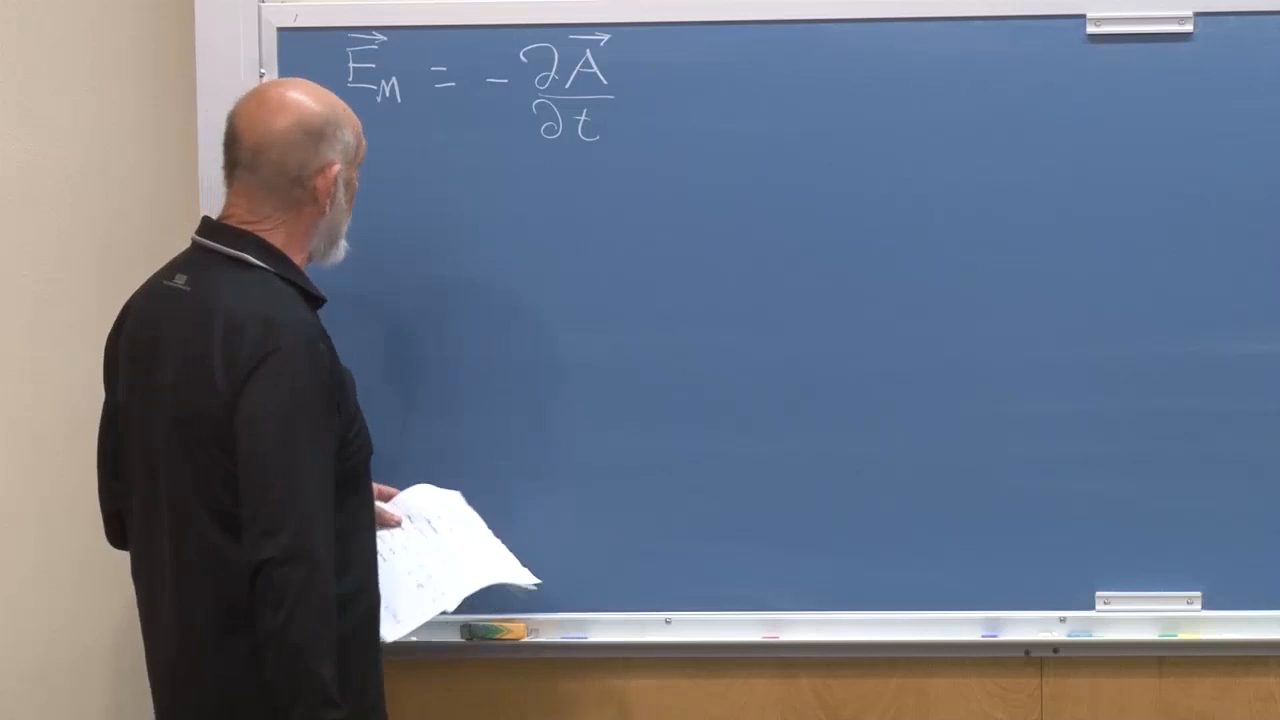
\includegraphics[width=\linewidth]{lecture_10_figure_02.png}\caption{역학적 운동량을 질량과 질량중심 속도의 곱으로 정의한다.}\par\smallskip
\textit{강의 영상 시각: 00:11:15.}\end{figure}

\subsection{정준 운동량}

역학이 다음과 같이 기술된다고 하자.
\(L(q_i,\dot q_i)\). \(q_i\)에 켤레인 정준 운동량은 다음과 같다.
\begin{equation}
p_i=\frac{\partial L}{\partial\dot q_i}.
\label{eq:canonical-momentum}
\end{equation}
\begin{equation}
L=\frac12 m\dot{\mathbf x}^{\,2}-V(\mathbf x),
\label{eq:simple-particle-lagrangian}
\end{equation}의 경우에는 \(\mathbf p=m\dot{\mathbf x}\)이므로 정준 운동량과 역학적 운동량이 우연히 일치한다.

\begin{figure}[H]\centering
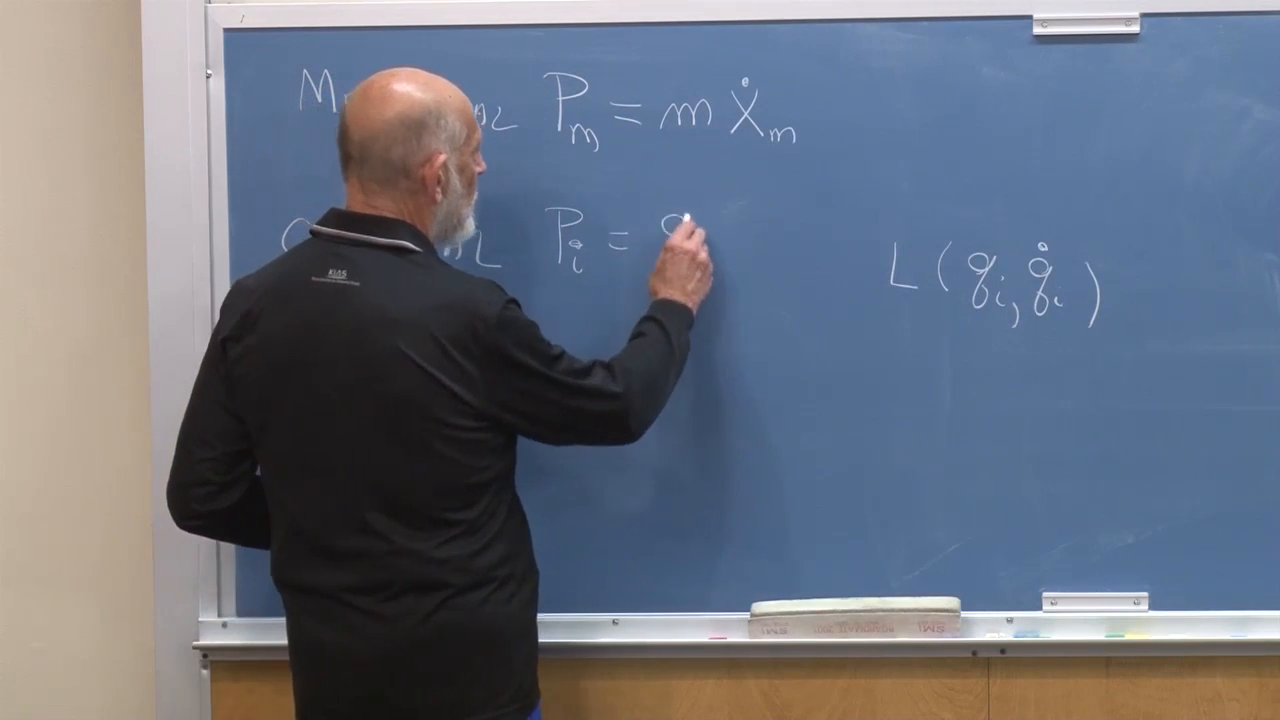
\includegraphics[width=\linewidth]{lecture_10_figure_03.png}\caption{단순한 입자 라그랑지안과 나란히 나타낸 역학적 운동량과 정준 운동량.}\par\smallskip
\textit{강의 영상 시각: 00:13:40.}\end{figure}

자기장 속의 하전 입자는 유용한 반례다. 칠판에 적은 부호 규약을 따르면
\begin{equation}
L=\frac12m\dot{\mathbf x}^{\,2}-V(\mathbf x)
  -e\,\dot{\mathbf x}\cdot\mathbf A(\mathbf x),
\label{eq:magnetic-particle-lagrangian}
\end{equation}
따라서
\begin{equation}
p_i=m\dot x_i-eA_i.
\label{eq:magnetic-canonical-shift}
\end{equation}
전하 또는 상호작용 항의 규약을 바꾸면 식에 나타나는 부호는 달라지지만, 핵심은 같다. 정준 운동량에는 벡터 퍼텐셜의 기여가 들어가며, 단순히 \(m\dot x_i\)인 것은 아니다. 해밀턴 방정식은 정준 변수를 사용한다. 나중에 장에 의존하는 항을 방정식의 반대편으로 옮기면 뉴턴 역학처럼 보이는 가속도 식을 얻을 수 있지만, 그렇게 식을 정리해도 정의 자체는 바뀌지 않는다.

\begin{figure}[H]\centering
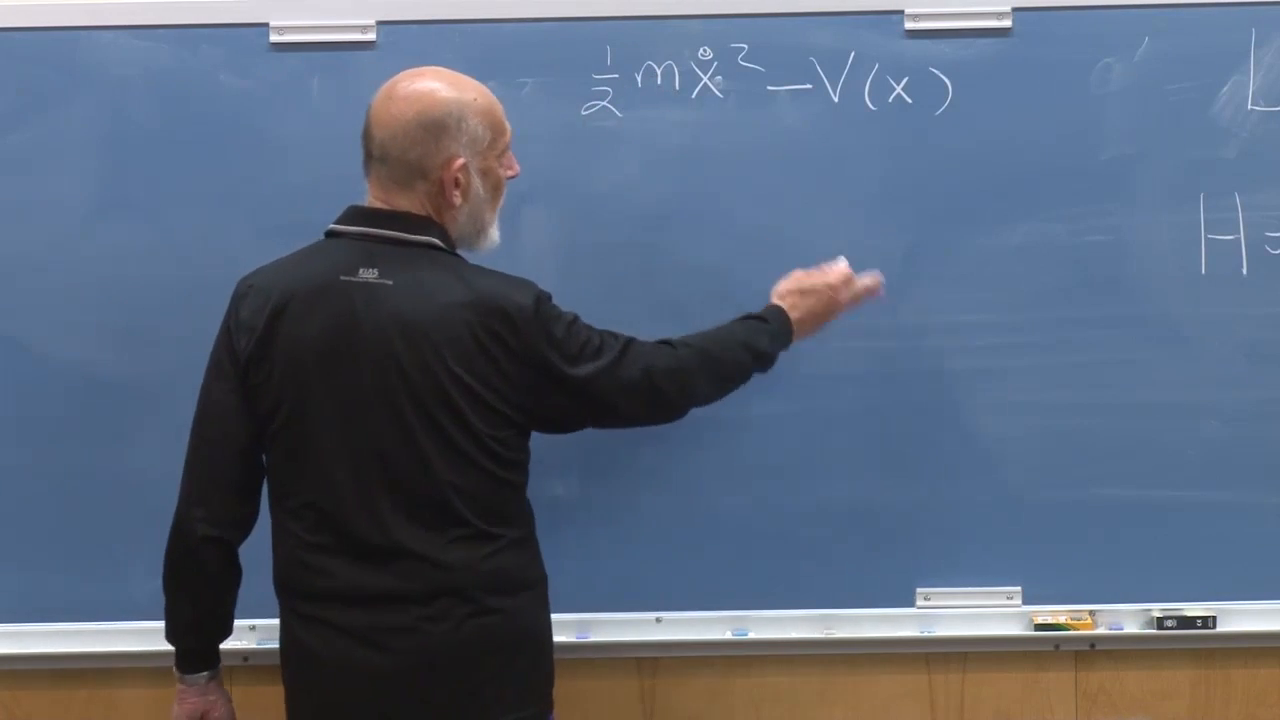
\includegraphics[width=\linewidth]{lecture_10_figure_04.png}\caption{벡터 퍼텐셜 항 때문에 정준 운동량은 역학적 운동량과 달라진다.}\par\smallskip
\textit{강의 영상 시각: 00:15:50.}\end{figure}

\subsection{뇌터 운동량}

세 번째 운동량은 공간 병진 대칭성에 대응하는 보존 전하다. 라그랑지안을 불변으로 두는 무한소 대칭 변환
\begin{equation}
q_i\longrightarrow q_i+\delta q_i
\end{equation}
에 대해 뇌터 정리는 무한소 매개변수의 정규화에 따라 다음을 준다.
\begin{equation}
Q=\sum_i p_i\,\delta q_i.
\label{eq:noether-charge-mechanics}
\end{equation}
여기에 나타나는 \(p_i\)는 정준 운동량이다. 대칭이 균일 병진이고 정준 운동량이 역학적 운동량과 우연히 같다면, \(Q\)는 익숙한 전체 운동량으로 환원된다. 더 복잡한 계에서는 그 일치를 가정하지 말고 증명해야 한다.

\begin{figure}[H]\centering
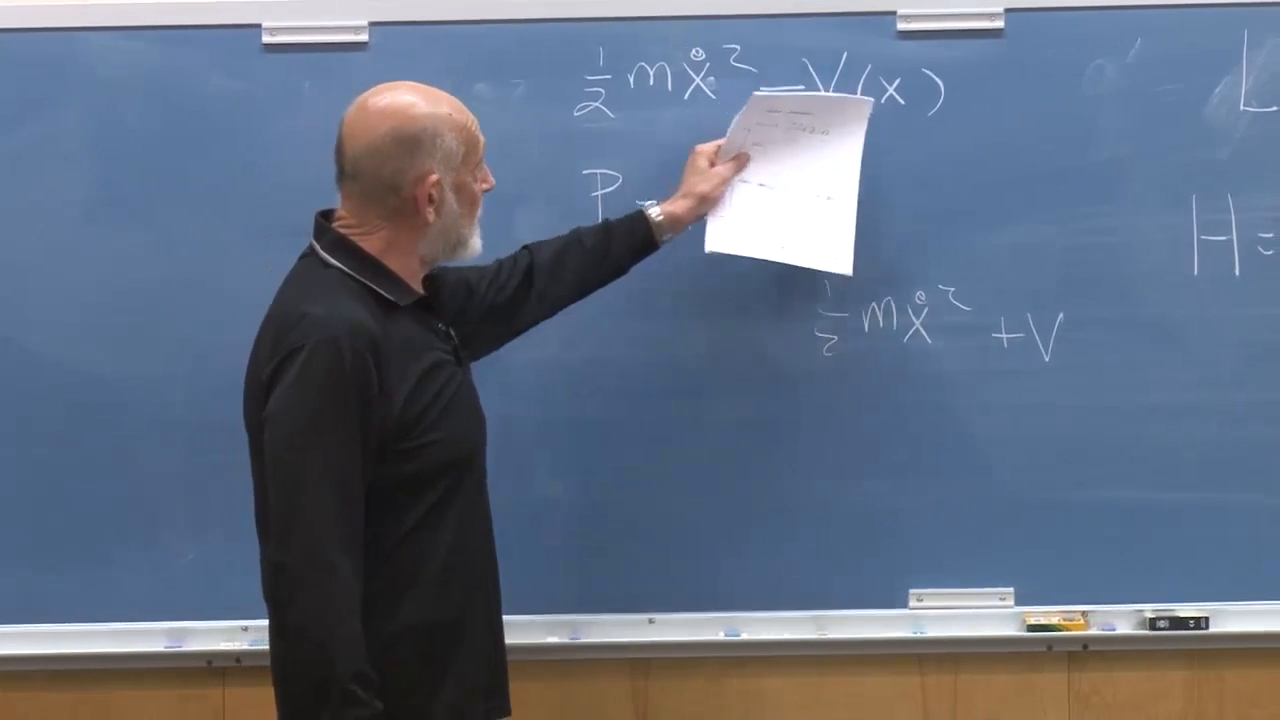
\includegraphics[width=\linewidth]{lecture_10_figure_05.png}\caption{정준 운동량과 좌표의 무한소 변화로 구성한 뇌터 전하.}\par\smallskip
\textit{강의 영상 시각: 00:19:00.}\end{figure}

\section{해밀토니안으로서의 에너지}

공간 병진은 운동량으로 이어지고, 시간 병진은 에너지로 이어진다. 라그랑지안이 시간에 명시적으로 의존하지 않으면 해밀토니안
\begin{equation}
H=\sum_i p_i\dot q_i-L
\label{eq:hamiltonian-definition}
\end{equation}
은 보존된다. 이것은 라그랑지안의 르장드르 변환이지, 식을 보고 부호를 바꾸는 규칙이 아니다.

\begin{figure}[H]\centering
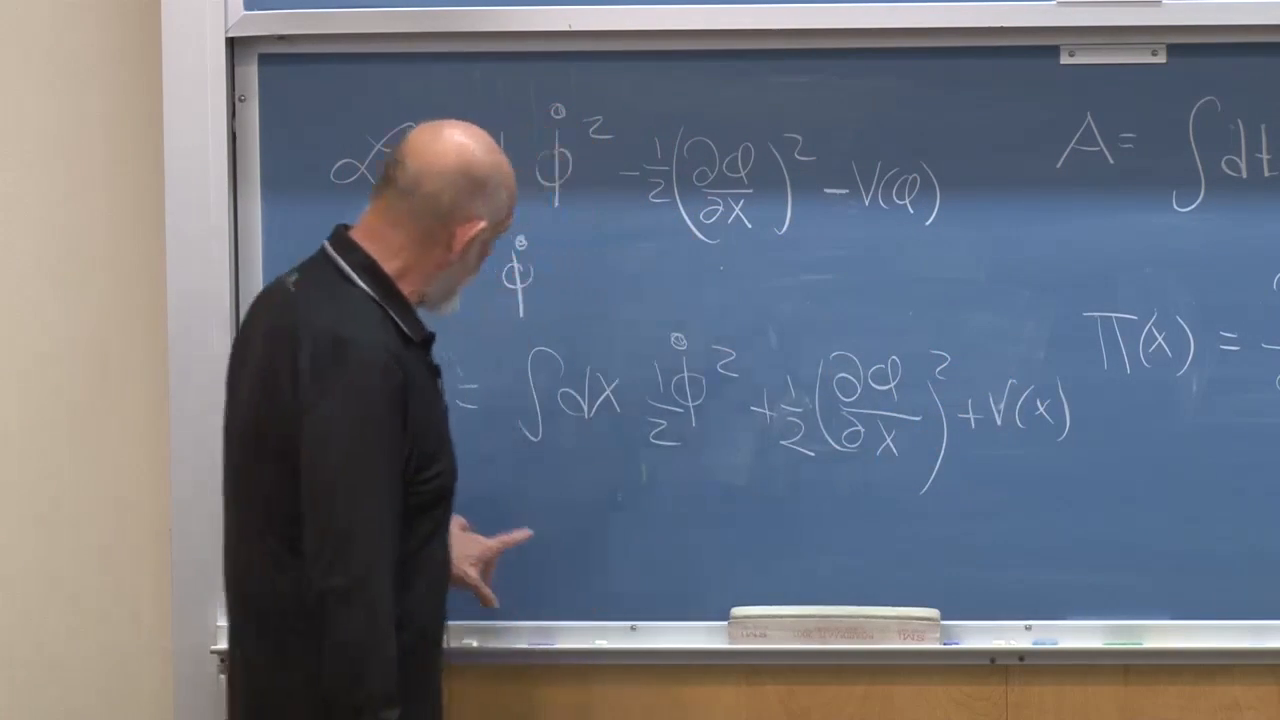
\includegraphics[width=\linewidth]{lecture_10_figure_06.png}\caption{일반적인 라그랑지안의 르장드르 변환으로 쓴 해밀토니안.}\par\smallskip
\textit{강의 영상 시각: 00:22:55.}\end{figure}

입자 하나의 예에서는
\begin{align}
p&=m\dot x,
\nonumber\\
H&=p\dot x-L\\
&=m\dot x^2
  -\left(\frac12m\dot x^2-V(x)\right)\\
&=\frac12m\dot x^2+V(x).
\label{eq:particle-hamiltonian}
\end{align}
따라서 라그랑지안은 운동에너지에서 퍼텐셜 에너지를 뺀 것이고, 해밀토니안은 운동에너지와 퍼텐셜 에너지를 더한 것이다.

\begin{figure}[H]\centering
\includegraphics[width=\linewidth]{lecture_10_figure_07.png}\caption{입자 계산을 통해 \(H=T+V\)가 \(H=p\dot x-L\)에서 어떻게 나오는지 보인다.}\par\smallskip
\textit{강의 영상 시각: 00:24:20.}\end{figure}

속도에 대한 모든 의존성이 표준적인 양의 이차 운동에너지 항이고 나머지 항에는 속도가 들어 있지 않다면, 속도가 없는 부분의 부호를 바꾸어 해밀토니안을 바로 읽어 낼 수 있다. 이 지름길은 앞으로 여러 번 쓰일 것이다. 여기서 다루는 예에서는 르장드르 변환이 이처럼 단순한 형태이므로 이 방법이 안전하다.

\section{장은 공간의 각 점에 연속적으로 무한히 많은 좌표가 있는 역학계다}

장 이론의 역학적 구조를 드러내기 위해 관성계를 하나 정하고, 잠시 각 식에 로런츠 공변성이 명시적으로 드러나야 한다는 요구를 내려놓자. 고전역학에는 시간축과 좌표 \(q_i(t)\)가 있다. 스칼라장에는 시간축과 좌표 \(\phi(\mathbf x,t)\)가 있다. 이산 표지 \(i\)가 연속 표지 \(\mathbf x\)로 바뀌었을 뿐이다.
\begin{equation}
q_i(t)\quad\longrightarrow\quad\phi(\mathbf x,t).
\label{eq:discrete-to-field}
\end{equation}
공간의 각 점에서 장이 갖는 값은 자유도 하나에 해당한다. 여기서 \(\mathbf x\)는 어떤 자유도를 가리키는 표지이지, 그 자체가 일반화 좌표는 아니다.

\begin{figure}[H]\centering
\includegraphics[width=\linewidth]{lecture_10_figure_08.png}\caption{공간 격자를 이용해 각 점의 장 값을 별도의 역학적 자유도로 나타낸 그림.}\par\smallskip
\textit{강의 영상 시각: 00:30:15.}\end{figure}

\begin{classroomqa}\audiencequestion{처음부터 장을 \(\phi(\mathbf x,t)\)라고 쓰면 안 되나요?}\lecturerresponse{그것이 완전한 표기법이다. 임시 표기 \(\phi(\mathbf x)\)는 흔히 \(q_i\)라고 쓰면서 각 \(q_i\)가 시간에 따라 변한다는 점을 염두에 두는 것처럼, 공통된 시간 인자를 생략한다. 표지 \(i\), 또는 이제는 \(\mathbf x\)가 논의 중인 자유도가 무엇인지 알려 준다. \lecturetimestamp{00:32:43}}\end{classroomqa}

\begin{classroomqa}\audiencequestion{서로 이웃한 점의 장 값은 정말 독립적인 좌표인가요? 연속성은 무엇이 보장하나요?}\lecturerresponse{이 값들은 독립적인 정준 좌표다. 이웃한 점들의 값을 서로 같게 두어 매끄러움을 강제하는 것은 아니다. 매끄러움은 동역학적으로 선택된다. 해밀토니안에는 양의 기울기 에너지 항이 있으므로, 거리가 점점 작아지는 두 점 사이에 고정된 불연속이 있으면 에너지 비용이 계속 커진다. 따라서 유한 에너지인 배치는 연속체 극한에서 매끄럽다. \lecturetimestamp{00:33:09}}\end{classroomqa}

공간 미분을 쓰면 이웃한 자유도 사이의 결합이 명시적으로 드러난다. 격자 간격이 \(\epsilon\)일 때,
\begin{equation}
\partial_x\phi(x,t)
  =\lim_{\epsilon\to0}
   \frac{\phi(x+\epsilon,t)-\phi(x,t)}{\epsilon}.
\label{eq:field-finite-difference}
\end{equation}
이 식은 서로 가까운 두 좌표에 의존하지만 일반화 속도는 포함하지 않는다. 역학적 비유에서 이것은 라그랑지안의 좌표 의존성에 해당하며 \(\dot q_i\) 의존성에는 해당하지 않는다.

\begin{figure}[H]\centering
\includegraphics[width=\linewidth]{lecture_10_figure_09.png}\caption{격자에서 이웃한 장 값의 차로 나타낸 공간 미분.}\par\smallskip
\textit{강의 영상 시각: 00:31:40.}\end{figure}

이제 작용을 명시적인 역학 형태로 쓸 수 있다.
\begin{align}
S&=\int dt\,L,
\nonumber\\
L&=\int d^3x\,
\mathcal L\!\left(
\phi,\dot\phi,\boldsymbol{\nabla}\phi
\right),
\nonumber\\
S&=\int dt\,d^3x\,
\mathcal L\!\left(
\phi,\dot\phi,\boldsymbol{\nabla}\phi
\right).
\label{eq:field-action-split}
\end{align}
필기체 문자 \(\mathcal L\)는 라그랑지안 밀도다. 이를 공간에 대해 적분하면 시간에 대해 다시 적분하는 보통의 라그랑지안을 얻는다. 국소 이론에서는 각 점의 장과 그 점에서의 미분을 통해서만 점들 사이에 결합이 생긴다. 시간과 공간을 분리하면 잠시 로런츠 공변성이 드러나지 않지만, 역학적 구조는 명확해진다.

\begin{figure}[H]\centering
\includegraphics[width=\linewidth]{lecture_10_figure_10.png}\caption{시간 적분과 라그랑지안 밀도의 공간 적분으로 나누어 쓴 장의 작용.}\par\smallskip
\textit{강의 영상 시각: 00:36:40.}\end{figure}

\section{정준 장 운동량과 해밀토니안 밀도}

장 좌표의 속도는 \(\dot\phi(\mathbf x,t)\)이다. 즉, 한 고정된 점에서 장이 시간에 따라 변하는 비율이다. 한 공간점에서 다른 공간점으로 이동하는 운동을 뜻하지 않는다. 따라서 장에 켤레인 정준 운동량 자체도 장이다.
\begin{equation}
\Pi(\mathbf x,t)
 =\frac{\partial\mathcal L}{\partial\dot\phi(\mathbf x,t)}.
\label{eq:field-canonical-momentum}
\end{equation}
여러 장 \(\phi_a\)이 있으면 각각에 대해 운동량 장 \(\Pi_a\)가 하나씩 있다.

르장드르 변환의 이산 합은 공간 적분으로 바뀐다.
\begin{align}
H
 &=\int d^3x\,
   \left[\Pi\dot\phi-\mathcal L\right]
  =\int d^3x\,\mathcal H,
\nonumber\\
\mathcal H
 &=\Pi\dot\phi-\mathcal L .
\label{eq:field-hamiltonian-density}
\end{align}
적분 안의 양이 에너지 밀도다.

\begin{figure}[H]\centering
\includegraphics[width=\linewidth]{lecture_10_figure_11.png}\caption{장에 대한 르장드르 변환과 이를 국소 에너지 밀도의 적분으로 해석한 식.}\par\smallskip
\textit{강의 영상 시각: 00:42:40.}\end{figure}

\begin{classroomqa}\audiencequestion{한 점에서 전체 라그랑지안을 \(\dot\phi\)에 대해 미분한 것을 그 점의 국소 밀도에 대한 미분으로 바꾸어도 되는 이유는 무엇인가요?}\lecturerresponse{공간 적분을 연속적인 합이라고 생각하면 된다. 여기서 가정한 국소성에 따르면 속도 \(\dot\phi(\mathbf x)\)는 바로 그 점에 해당하는 항에만 나타난다. 그 속도 하나에 대해 미분하면 다른 모든 항은 사라진다. 공간 미분은 이웃한 장 값들을 결합할 수 있지만, 이 이론에서는 이웃한 점의 시간 미분을 끌어들이지 않는다. \lecturetimestamp{00:51:56}}\end{classroomqa}

\subsection{스칼라장}

공간 차원이 하나일 때 다음을 취하자.
\begin{equation}
\mathcal L
 =\frac12\dot\phi^2
  -\frac12(\partial_x\phi)^2
  -V(\phi).
\label{eq:scalar-field-lagrangian}
\end{equation}
이는 앞서 사용한 로런츠 스칼라를 공변성이 명시적으로 드러나지 않는 형태로 쓴 것이다. 시간 미분과 공간 미분 사이의 상대적인 마이너스 부호는 민코프스키 계량에서 나온다. 정준 운동량은
\begin{equation}
\Pi=\dot\phi,
\label{eq:scalar-pi}
\end{equation}
이고 해밀토니안은 다음과 같다.
\begin{equation}
H=\int dx\,
\left[
\frac12\dot\phi^2
+\frac12(\partial_x\phi)^2
+V(\phi)
\right].
\label{eq:scalar-field-hamiltonian}
\end{equation}
계산 도중 퍼텐셜을 잠시 \(V(x)\)라고 불렀다가 수강생들이 \(V(\phi)\)로 바로잡았다. 장을 통해 간접적으로 위치에 의존할 수는 있지만, 병진 불변인 이론에서는 지정된 외부 \(x\) 의존성이 없다.

\begin{figure}[H]\centering
\includegraphics[width=\linewidth]{lecture_10_figure_12.png}\caption{스칼라 라그랑지안 밀도, 켤레 운동량, 양의 해밀토니안을 한 칠판에 모아 쓴 모습.}\par\smallskip
\textit{강의 영상 시각: 00:47:05.}\end{figure}

시간 미분이 전혀 없는 부분 전체가 퍼텐셜 에너지 역할을 한다. 여기에는 \(V(\phi)\)와 기울기 에너지 \(\frac12(\partial_x\phi)^2\)가 모두 포함된다. 라그랑지안은 어느 부호를 가져도 되지만, 안정한 에너지는 아래로 유계여야 한다.

\begin{classroomqa}\audiencequestion{\(V(\phi)\)는 음수일 수 있나요?}\lecturerresponse{그렇다. 유한한 하한이 있다면 상수를 더해 고전적 장 방정식을 바꾸지 않고도 최솟값을 0으로 만들 수 있다. 아래로 유계가 아닌 퍼텐셜은 불안정성을 뜻한다. 장의 에너지를 한계 없이 낮출 수 있기 때문이다. 안정한 진공은 상수인 장이 이동된 퍼텐셜의 최솟값에 놓인 상태다. \lecturetimestamp{00:49:03}}\end{classroomqa}

앞서 던진 연속성 질문에 이제 정량적으로 답할 수 있다. 격자 간격 \(\epsilon\)을 사이에 둔 불연속 \(\Delta\phi\)은 다음 기여를 한다.
\begin{equation}
\frac12(\partial_x\phi)^2
\sim\frac12\left(\frac{\Delta\phi}{\epsilon}\right)^2.
\label{eq:gradient-cost}
\end{equation}
\(\epsilon\to0\)일 때 고정된 불연속은 임의로 큰 에너지 밀도를 만든다. 따라서 유한 에너지는 들쭉날쭉한 배치를 억제한다.

\begin{figure}[H]\centering
\includegraphics[width=\linewidth]{lecture_10_figure_13.png}\caption{칠판 그림에서 매끄러운 장과 급격한 변화를 대비하며 유지한 스칼라 에너지 식.}\par\smallskip
\textit{강의 영상 시각: 00:54:20.}\end{figure}

\section{국소 에너지와 \texorpdfstring{\(T^{00}\)}{00}의 의미}

에너지 밀도에는 간결한 이름이 붙어 있다.
\begin{equation}
T^{00}=\mathcal H=\Pi\dot\phi-\mathcal L.
\label{eq:T00-definition}
\end{equation}
위첨자 0이 두 개 붙은 것은 서로 별개의 두 가지 진술을 나타낸다. 에너지는 에너지--운동량 사벡터의 시간 성분 \(P^0\)이고, 밀도는 보존 전류의 시간 성분이다. 따라서 \(T^{00}\)는 사차원 운동량의 시간 성분 밀도다.

\begin{figure}[H]\centering
\includegraphics[width=\linewidth]{lecture_10_figure_14.png}\caption{국소적으로 나타내고 \(T^{00}\)와 동일시한 장의 에너지.}\par\smallskip
\textit{강의 영상 시각: 01:00:00.}\end{figure}

상대론적 국소 이론에서 보존은 하나의 전역적인 수가 변하지 않는다는 말에 그치지 않는다. 에너지가 실험실에서 사라졌다가 알파 센타우리에서 다시 나타날 수는 없다. 어떤 영역 안에서 일어난 변화는 그 경계를 통과하는 플럭스로 설명되어야 한다. 국소 형태로 쓰면
\begin{equation}
\partial_\mu T^{\mu\nu}=0,
\label{eq:stress-energy-continuity}
\end{equation}
첫 번째 첨자는 밀도 또는 플럭스의 방향을, 두 번째 첨자는 전달되는 성분 \(P^\nu\)을 나타낸다.

\begin{classroomqa}\audiencequestion{\(T^{00}\)를 밀도라고 부른다는 것은 전체 에너지를 이것의 적분으로 구한다는 뜻인가요?}\lecturerresponse{그렇다.
\(E=P^0=\int d^3x\,T^{00}\). 국소 밀도는 장에 대한 르장드르 변환의 적분함수다. 한 지점에서의 변화는 이웃한 지점들 사이를 흐르는 에너지 전류로 보상된다. \lecturetimestamp{00:59:06}}\end{classroomqa}

\section{공간 병진에서 나오는 운동량 밀도}

이제 이산 합을 공간 적분으로 바꾸어 뇌터 공식을 다시 보자. \(m\) 방향으로 작은 병진을 하면 수동적 규약에서 장은 다음과 같이 변한다.
\begin{equation}
\delta\phi
  =\phi(\mathbf x)-\phi(\mathbf x-\boldsymbol{\epsilon})
  =\epsilon^m\partial_m\phi+O(\epsilon^2),
\label{eq:translated-field-change}
\end{equation}
능동 병진과 수동 병진을 서로 바꾸면 전체 부호도 바뀐다. 이 규약을 정하면 물리적 생성자가 정해진다. \(\epsilon^m\)을 묶어 내면 뇌터 운동량은 다음 구조를 갖는다.
\begin{equation}
P_m\ \propto\ \int d^3x\,\Pi\,\partial_m\phi.
\label{eq:scalar-noether-momentum}
\end{equation}

\begin{figure}[H]\centering
\includegraphics[width=\linewidth]{lecture_10_figure_15.png}\caption{병진된 장 분포와 그 무한소 변화를 나타내는 미분.}\par\smallskip
\textit{강의 영상 시각: 01:04:20.}\end{figure}

\begin{classroomqa}\audiencequestion{무한소 병진량 \(\epsilon\)을 운동량 식에 남겨 두지 않은 이유는 무엇인가요?}\lecturerresponse{뇌터 전하는 먼저 \(\epsilon\)에 비례하는 형태로 얻어진다. 운동량은 임의의 병진 매개변수에 곱해지는 계수로 정의하므로, \(\epsilon\)로 나누어 없앤다. 보존량에 고정된 상수를 곱해도 보존 여부는 달라지지 않지만, 계수를 추출하면 표준 정규화를 얻는다. \lecturetimestamp{01:04:45}}\end{classroomqa}

\begin{classroomqa}\audiencequestion{연속체 적분에서 병진 간격이 \(dx\)가 되나요?}\lecturerresponse{두 양은 서로 다른 극한에서 나온다. 공간 표지로 붙은 자유도들의 합을 적분으로 바꿀 때 측도 \(dx\)가 생긴다. 병진 매개변수 \(\epsilon\)는 대칭 변환을 나타내며 뇌터 전하에서 인수로 묶어 낸다. 중간 단계의 추론에서 둘 다 무한소이지만, 역할은 서로 다르다. \lecturetimestamp{01:05:16}}\end{classroomqa}

강의의 표기법에서 운동량의 \(m\)성분 밀도는 다음과 같다.
\begin{equation}
T^{0m}=\Pi\,\partial_m\phi,
\label{eq:scalar-momentum-density}
\end{equation}
병진 부호 규약은 위와 같이 정했다. 스칼라 이론에서는 \(\Pi=\dot\phi\)이므로 이는 다음에 비례한다.
\(\dot\phi\,\partial_m\phi\).

\begin{figure}[H]\centering
\includegraphics[width=\linewidth]{lecture_10_figure_16.png}\caption{칠판에 쓴 뇌터 운동량 밀도 \(T^{0m}=\Pi\,\partial_m\phi\).}\par\smallskip
\textit{강의 영상 시각: 01:07:10.}\end{figure}

이는 파동이 실제로 운반하는 운동량이다. 병진 불변성은 장, 입자, 전하원, 장치를 모두 함께 병진할 때만 성립한다. 자유롭게 매달린 판이 광 펄스를 흡수하면 판은 반동을 받는다. 보통 빛에서는 효과가 아주 작지만, 충분히 강한 레이저는 작은 표적을 압축할 만큼 큰 운동량을 전달할 수 있다. 보존되는 전체 운동량은 입자와 장을 함께 포함한다.

\subsection{뉴턴 방정식에 해당하는 것은 무엇인가?}

식~\eqref{eq:scalar-field-lagrangian}에서 유도한 장의 오일러--라그랑주 방정식은 다음과 같다.
\begin{equation}
\ddot\phi-\nabla^2\phi=-\frac{dV}{d\phi}.
\label{eq:scalar-equation-of-motion}
\end{equation}
이는 장 이론에서 뉴턴 법칙에 해당한다.

\begin{figure}[H]\centering
\includegraphics[width=\linewidth]{lecture_10_figure_17.png}\caption{해밀토니안 및 운동량 밀도와 나란히 나타낸 스칼라장 방정식.}\par\smallskip
\textit{강의 영상 시각: 01:12:55.}\end{figure}

\begin{classroomqa}\audiencequestion{장에 대해 뉴턴 법칙에 해당하는 것은 무엇인가요?}\lecturerresponse{오일러--라그랑주 장 방정식이다. 여기서는 힘 항 \(-V'(\phi)\)가 있는 파동 방정식이다. \(m\ddot x=-V'(x)\)에 해당하는 역할은 다음이 한다.
\(\ddot\phi-\nabla^2\phi=-V'(\phi)\)
\lecturetimestamp{01:11:48}}\end{classroomqa}

\begin{classroomqa}\audiencequestion{제안된 장 라그랑지안이 옳은지는 어떻게 알 수 있나요? 장 방정식을 이미 알아야 하나요?}\lecturerresponse{어느 방향으로도 진행할 수 있다. 역사적으로는 뉴턴이나 맥스웰의 경우처럼 실험에서 방정식을 추론한 다음 작용을 찾을 수 있다. 현대 이론에서는 장의 종류, 국소성, 대칭성, 허용되는 소수의 항에서 출발해 방정식을 유도하고 예측을 검증하는 경우가 많다. 여기 적힌 스칼라장은 기본 장을 나타낼 수도 있지만, 구성 입자들에서 연속체 작용을 유도한 밧줄의 횡변위를 나타낼 수도 있다. \lecturetimestamp{01:12:55}}\end{classroomqa}

\section{시간 성분 게이지에서의 전자기장}

앞서 구한 성분 \(T^{00}\)와 \(T^{0m}\)는 에너지--운동량 텐서에 속한다. 나머지 성분은 에너지와 운동량의 플럭스를 나타낸다. 이 텐서는 나중에 중력의 원천이 되지만, 당장은 전자기장이 구체적인 예를 제공한다.

기본 전자기 좌표는 사중 퍼텐셜 \(A_\mu\)이다. 게이지 자유도에 따라 다음과 같이 변환할 수 있다:
\begin{equation}
A_\mu\longrightarrow A'_\mu=A_\mu+\partial_\mu S
\label{eq:gauge-transformation-lecture10}
\end{equation}
이때 \(F_{\mu\nu}\)는 변하지 않는다. \(S\)가 다음 조건을 만족하도록 택하자:
\begin{equation}
\partial_tS=-A_0.
\label{eq:temporal-gauge-choice}
\end{equation}
예를 들어, 각 공간 위치에서 \(A_0\)를 시간에 대해 적분할 수 있다. 그러면 변환된 시간 성분은 사라진다:
\begin{equation}
A'_0=A_0+\partial_tS=0.
\label{eq:temporal-gauge}
\end{equation}
이것이 시간 게이지다. 이 게이지를 택하면 \(A_0\)는 동역학적 좌표 목록에서 제외되지만, 가우스 법칙은 제약 조건으로 남고 시간에 무관한 잔여 게이지 자유도도 남는다.

\begin{figure}[H]\centering
\includegraphics[width=\linewidth]{lecture_10_figure_18.png}\caption{\(A_0=0\)이 되도록 \(\partial_tS=-A_0\)를 풀어 이용한 게이지 자유도.}\par\smallskip
\textit{강의 영상 시각: 01:20:15.}\end{figure}

이제부터 \(\mathbf E\)는 표준 Maxwell 전기장을 뜻한다고 하자. 게이지를 고정하기 전에는
\begin{equation}
E_m=-\partial_tA_m+\partial_mA_0,
\qquad
\mathbf B=\boldsymbol{\nabla}\times\mathbf A.
\label{eq:E-B-general-potential}
\end{equation}
시간 성분 게이지에서는 다음처럼 단순해진다.
\begin{equation}
\mathbf E=-\dot{\mathbf A},
\qquad
\mathbf B=\boldsymbol{\nabla}\times\mathbf A.
\label{eq:E-B-temporal-gauge}
\end{equation}
\(\mathbf A\)의 시간 미분은 전기장을, 공간 미분은 자기장을 만든다.

\begin{figure}[H]\centering
\includegraphics[width=\linewidth]{lecture_10_figure_19.png}\caption{시간 성분 게이지에서의 전기장과 자기장: \(\mathbf E=-\dot{\mathbf A}\) 및 \(\mathbf B=\nabla\times\mathbf A\).}\par\smallskip
\textit{강의 영상 시각: 01:23:50.}\end{figure}

\section{전자기 정준 운동량과 에너지}

자유 Maxwell 라그랑지안 밀도는 다음과 같다.
\begin{equation}
\mathcal L_{\mathrm{EM}}
 =-\frac14F_{\mu\nu}F^{\mu\nu}
 =\frac12\left(\mathbf E^2-\mathbf B^2\right).
\label{eq:maxwell-lagrangian-energy-lecture}
\end{equation}
시간 성분 게이지에서는
\begin{equation}
\mathcal L_{\mathrm{EM}}
 =\frac12\dot{\mathbf A}^{\,2}
  -\frac12(\boldsymbol{\nabla}\times\mathbf A)^2.
\label{eq:maxwell-lagrangian-temporal}
\end{equation}
스칼라장과 정확히 같은 형태다. 시간 미분의 제곱에서 공간 미분의 제곱을 뺀다.

\begin{figure}[H]\centering
\includegraphics[width=\linewidth]{lecture_10_figure_20.png}\caption{\(\mathbf A\)의 공간 성분에 대한 역학적 장 라그랑지안으로 다시 쓴 Maxwell 라그랑지안.}\par\smallskip
\textit{강의 영상 시각: 01:28:10.}\end{figure}

각 성분 \(A_m\)에는 정준 운동량이 하나씩 대응한다.
\begin{equation}
\Pi_m
 =\frac{\partial\mathcal L_{\mathrm{EM}}}
        {\partial\dot A_m}
 =\dot A_m
 =-E_m.
\label{eq:em-canonical-momentum}
\end{equation}
이는 규약이 중요한 이유를 구체적으로 보여 준다. 앞서 사용한 반대 전기장 규약에서는 마지막 식에 나타나는 부호가 바뀌지만, 정준 미분 자체는 바뀌지 않는다.

\begin{figure}[H]\centering
\includegraphics[width=\linewidth]{lecture_10_figure_21.png}\caption{\(A_x,A_y,A_z\)에 대응하는 세 운동량 장. 각각 해당 시간 미분과 같으며, 따라서 표준 전기장의 음수다.}\par\smallskip
\textit{강의 영상 시각: 01:30:20.}\end{figure}

이제 해밀토니안의 지름길을 정당화할 수 있다. 시간 미분이 없는 항의 부호를 바꾸면 된다. 전자기 에너지 밀도는
\begin{equation}
T^{00}_{\mathrm{EM}}
 =\mathcal H_{\mathrm{EM}}
 =\frac12\left(\mathbf E^2+\mathbf B^2\right),
\label{eq:em-energy-density}
\end{equation}
이고 전체 에너지는
\begin{equation}
H_{\mathrm{EM}}
 =\int d^3x\,
\frac12\left(\mathbf E^2+\mathbf B^2\right).
\label{eq:em-total-energy}
\end{equation}
이다. 라그랑지안 밀도와 달리 에너지 밀도는 음수가 될 수 없다.

\begin{figure}[H]\centering
\includegraphics[width=\linewidth]{lecture_10_figure_22.png}\caption{양의 값을 갖는 전자기 해밀토니안 밀도 \(\frac12(\mathbf E^2+\mathbf B^2)\).}\par\smallskip
\textit{강의 영상 시각: 01:32:00.}\end{figure}

진공 속 평면파에서는 \(\mathbf E\perp\mathbf B\)이고 두 장은 같은 위상으로 진동한다. \(c=1\)인 단위계에서는 두 장의 크기가 같다. 따라서 전기장과 자기장이 파동 에너지를 똑같이 나누어 가진다.
\begin{equation}
u_E=\frac12\mathbf E^2,
\qquad
u_B=\frac12\mathbf B^2,
\qquad
u_E=u_B.
\label{eq:plane-wave-energy-halves}
\end{equation}

\section{전자기 운동량의 유도}

이제 뇌터 병진 공식을 세 장 \(A_m\)에 대해 합산해야 한다. 물리적 운동량이 파동의 진행 방향을 향하도록 병진 부호를 정하면, \(n\)성분은 다음과 같다.
\begin{equation}
P_n
 =\int d^3x\,E_m\,\partial_nA_m,
\label{eq:em-canonical-noether-momentum}
\end{equation}
여기서 \(m\)에 대해 합한다. 강의에서는 부호 문제를 의도적으로 짚고 넘어간다. 부호는 앞서 정한 전기장 규약과 능동 또는 수동 병진의 선택에 달려 있다. 게이지 불변인 물리적 결과로 부호를 확정할 수 있다.

\begin{figure}[H]\centering
\includegraphics[width=\linewidth]{lecture_10_figure_23.png}\caption{세 성분의 벡터 퍼텐셜로 확장한 스칼라장 뇌터 공식.}\par\smallskip
\textit{강의 영상 시각: 01:36:40.}\end{figure}

적분함수에는 여전히 물리장만이 아니라 게이지 퍼텐셜이 들어 있다. \(E_m\partial_mA_n\)를 더하고 빼면
\begin{align}
E_m\partial_nA_m
 &=
 E_m\left(\partial_nA_m-\partial_mA_n\right)
 +E_m\partial_mA_n.
\label{eq:add-subtract-em-momentum}
\end{align}
첫 번째 항은 외적이다.
\begin{equation}
E_m\left(\partial_nA_m-\partial_mA_n\right)
  =(\mathbf E\times\mathbf B)_n.
\label{eq:cross-product-component}
\end{equation}
두 번째 항에는 부분적분을 적용한다.
\begin{align}
\int d^3x\,E_m\partial_mA_n
 &=
\int_{\partial V}d\Sigma_m\,E_mA_n
-\int d^3x\,A_n\partial_mE_m.
\label{eq:em-momentum-integration-parts}
\end{align}
장이 경계에서 충분히 빨리 감소해 경계항이 사라지고, 전하원이 없는 영역이라 \(\boldsymbol{\nabla}\cdot\mathbf E=0\)이면 두 번째 항은 기여하지 않는다.

\begin{figure}[H]\centering
\includegraphics[width=\linewidth]{lecture_10_figure_24.png}\caption{부분적분으로 더한 항을 \(\nabla\cdot\mathbf E\)로 옮긴 모습.}\par\smallskip
\textit{강의 영상 시각: 01:40:00.}\end{figure}

따라서 강의의 단위계에서 장의 전체 운동량은 다음과 같다.
\begin{equation}
\mathbf P_{\mathrm{EM}}
 =\int d^3x\,\mathbf E\times\mathbf B,
\qquad
\mathbf g_{\mathrm{EM}}
 =\mathbf E\times\mathbf B,
\label{eq:em-momentum-density}
\end{equation}
벡터 \(\mathbf g_{\mathrm{EM}}\)는 전자기 운동량 밀도다.

\begin{figure}[H]\centering
\includegraphics[width=\linewidth]{lecture_10_figure_25.png}\caption{게이지 퍼텐셜로 나타낸 식을 게이지 불변 운동량 \(\int d^3x\,\mathbf E\times\mathbf B\)로 정리했다.}\par\smallskip
\textit{강의 영상 시각: 01:41:10.}\end{figure}

\begin{classroomqa}\audiencequestion{어디에서 \(\boldsymbol{\nabla}\cdot\mathbf E=0\)를 사용했나요? 전하가 있으면 어떻게 되나요?}\lecturerresponse{부분적분 뒤에 남는 부피항을 없앨 때 사용했다. 따라서 위에서 제시한 장만을 다루는 유도는 자유 전자기파에 적용된다. 전하가 있으면 그 항은 0이 아니므로 하전 물질의 운동량도 포함해야 한다. 병진 불변성과 운동량 보존은 물질--장 전체 계에 관한 것이다. \lecturetimestamp{01:41:55}}\end{classroomqa}

\subsection{파동 운동량의 방향}

평면파에서 \(\mathbf E\), \(\mathbf B\), 진행 방향은 오른손 좌표계를 이룬다. 반 파장만큼 진행하면 \(\mathbf E\)와 \(\mathbf B\)가 모두 방향을 바꾼다.
\begin{equation}
(-\mathbf E)\times(-\mathbf B)
 =\mathbf E\times\mathbf B.
\label{eq:poynting-sign-reversal}
\end{equation}
따라서 운동량 밀도는 진동 내내 한 방향을 유지하며, 그 방향은 파동의 진행 방향이다.

\begin{figure}[H]\centering
\includegraphics[width=\linewidth]{lecture_10_figure_26.png}\caption{평면파의 기하: 전기장과 자기장은 함께 방향을 바꾸지만, 두 장의 외적은 계속 진행축을 향한다.}\par\smallskip
\textit{강의 영상 시각: 01:43:10.}\end{figure}

이 때문에 빛의 압력은 실제로 존재한다. 흡수되면 장의 운동량이 물질로 전달되고, 반사되면 빛의 운동량 방향이 뒤집혀 반사체에 법선 성분의 두 배까지 전달될 수 있다.

\section{퍼텐셜과 관측 가능한 장의 접점}

\(A_\mu\)와 관측 가능한 장이 만나는 접점은 어디일까? 수업을 마무리하며 학생들은 이 질문을 던진다. 그 접점은 바로 다음과 같다.
\begin{align}
E_n&=-\partial_tA_n+\partial_nA_0,
\nonumber\\
B_n&=\epsilon_{nmk}\partial_mA_k.
\label{eq:potential-field-contact}
\end{align}
시간 게이지를 택하면 \(A_0\) 항은 사라지지만 물리적 장은 바뀌지 않는다.

\begin{figure}[H]
\centering
\includegraphics[width=\linewidth]{lecture_10_figure_27.png}
\caption{시간 게이지에서 계산한 뒤 복원한 일반적인 전기장 관계식과, 그 아래에 다시 제시한 공변 스칼라 라그랑지안.}
\par\smallskip
\textit{강의 화면: 01:45:40.}
\end{figure}

\begin{classroomqa}
\audiencequestion{벡터 퍼텐셜과 전기장 및 자기장은 정확히 어떻게 연결되는가?}
\lecturerresponse{전기장은 공간 퍼텐셜의 시간 미분과 \(A_0\)의 공간 미분을 결합한 것이고, 자기장은 공간 퍼텐셜의 회전이다. 시간 게이지에서는 다음처럼 간단해진다.
\(\mathbf E=-\dot{\mathbf A}\) 그리고
\(\mathbf B=\nabla\times\mathbf A\).
\lecturetimestamp{01:44:15}}
\end{classroomqa}

\begin{classroomqa}
\audiencequestion{퍼텐셜은 \(\mathbf E\)와 \(\mathbf B\)보다 더 근본적인가?}
\lecturerresponse{작용과 게이지 원리는 \(A_\mu\)를 사용해 가장 자연스럽게 정식화되므로, 퍼텐셜은 구조적으로 근본적인 변수다. 그러나 \(A_\mu\)는 유일하지 않다. 게이지 변환으로 서로 연결된 퍼텐셜은 같은 물리를 나타내며, 국소 장은 게이지 불변이다. 두 진술은 서로 양립한다. 근본 변수라고 해서 반드시 직접 관측 가능해야 하는 것은 아니다. \lecturetimestamp{01:46:36}}
\end{classroomqa}

\begin{classroomqa}
\audiencequestion{게이지 퍼텐셜 자체가 힘을 가할 수 있는가?}
\lecturerresponse{게이지에 의존하는 표현으로부터 게이지에 의존하는 측정 가능 힘이 생길 수는 없다. 작용에서는 전하를 띤 물질이 퍼텐셜과 결합하지만, 고전적인 로런츠 힘은 게이지 불변인 전기장과 자기장만으로 완전히 쓸 수 있다.
\lecturetimestamp{01:47:49}}
\end{classroomqa}

\begin{classroomqa}
\audiencequestion{전기장과 자기장이 서로 교차하고 정적이라면,
그 운동량은 반드시 영이어야 하는가?}
\lecturerresponse{장 자체의 운동량은 반드시 영일 필요는 없다:
\(\mathbf E\times\mathbf B\)는 두 장이 모두 시간에 따라 변하지 않더라도 영이 아닐 수 있다. 닫힌 정적 장치에서 전체 운동량 수지에는 전하, 전류, 지지 구조물, 그리고 기계적 운동량이나 숨은 운동량도 포함된다. 전체 운동량이 균형을 이루어야 한다는 간단한 강의실 답변은 올바른 보존 법칙의 진술이다. 장의 기여분만 영이라고 두는 것은 지나치게 강한 주장이다.
\lecturetimestamp{01:48:01}}
\end{classroomqa}

\section{하나의 텐서, 포인팅 벡터의 두 가지 의미}

에너지--운동량 텐서는 모든 밀도와 플럭스를 한데 정리한다.
\begin{align}
T^{00}&=\text{energy density},\\
T^{0i}&=\text{\(i\)-momentum density},\\
T^{i0}&=\text{energy flux in the \(i\)-direction},\\
T^{ij}&=\text{\(j\)-momentum flux in the \(i\)-direction}.
\label{eq:stress-energy-components}
\end{align}
예를 들어 \(T^{31}\)는 단위 시간당 \(x\)-운동량이 \(z\) 방향을 법선으로 하는 단위 면적을 통과하는 양이다. 공간 성분 블록 \(T^{ij}\)은 응력 텐서다.

\begin{figure}[H]
\centering
\includegraphics[width=\linewidth]{lecture_10_figure_28.png}
\caption{칠판에는 밀도와 플럭스 성분이 에너지--운동량 텐서로 정리되기 시작한다.}
\par\smallskip
\textit{강의 화면: 01:51:10.}
\end{figure}

여기서 다루는 상대론적 계에서는 물리적인 에너지--운동량 텐서를 대칭으로 택할 수 있다.
\begin{equation}
T^{\mu\nu}=T^{\nu\mu}.
\label{eq:stress-energy-symmetry}
\end{equation}
따라서
\begin{equation}
T^{0i}=T^{i0}.
\label{eq:momentum-density-energy-flux}
\end{equation}
\(i\)-운동량의 밀도는 \(c=1\)일 때 \(i\) 방향의 에너지 플럭스와 같다. 이것이 청중의 마지막 질문, 곧 포인팅 벡터가 실제로 단위 면적당 전력인지에 대한 답이다.

\begin{classroomqa}
\audiencequestion{\(\mathbf E\times\mathbf B\)는 운동량 밀도가 아니라 전력 밀도인가?}
\lecturerresponse{둘 다다. \(T^{\mu\nu}\)의 대칭성에 따라 운동량 밀도 \(T^{0i}\)는 에너지 플럭스 \(T^{i0}\)와 같다. 그러므로 \(\mathbf S=\mathbf E\times\mathbf B\)는 단위 시간당 단위 면적을 통과하는 에너지이며, \(c=1\) 단위계에서는 단위 부피당 운동량이기도 하다. 통상적인 단위를 복원하면 \(\mathbf g=\mathbf S/c^2\).
\lecturetimestamp{01:48:20}}
\end{classroomqa}

\begin{figure}[H]
\centering
\includegraphics[width=\linewidth]{lecture_10_figure_29.png}
\caption{운동량 밀도와 에너지 플럭스를 같게 두는 대칭 텐서 관계를 칠판에 포인팅 벡터로 표시했다.}
\par\smallskip
\textit{강의 화면: 01:53:50.}
\end{figure}

\section{일반상대성이론으로 가는 다리}

강의는 고전역학, 장 이론, 전자기학을 하나의 구조로 엮으며 마무리된다.
\begin{enumerate}
\item 시간 병진 대칭성은 해밀토니안과 에너지를 준다.
\item 공간 병진 대칭성은 뇌터 운동량을 준다.
\item 이산적인 좌표를 공간상의 각 점에 붙은 장으로 바꾸면 합은 적분으로, 보존량은 국소 밀도로 바뀐다.
\item 게이지를 고정하면 관측량을 바꾸지 않은 채 맥스웰 장의 역학적 좌표를 드러낼 수 있다.
\item 맥스웰 해밀토니안은 다음을 주고,
\(\frac12(\mathbf E^2+\mathbf B^2)\) 공간 병진은 다음을 준다.
\(\mathbf E\times\mathbf B\).
\item 대칭 에너지--운동량 텐서는 에너지 밀도, 운동량 밀도, 에너지 플럭스, 응력을 하나로 통합한다.
\end{enumerate}

다음 단계에서 필요한 물리량이 바로 이것이다. 일반상대성이론에서 에너지--운동량 텐서는 아인슈타인 장방정식의 원천으로 나타난다. 따라서 마지막 강의는 전자기학 계산을 덧붙이는 데 그치지 않고, 물질과 장이 시공간에 어떻게 곡률을 부여하는지를 기술하는 언어를 마련했다.

\end{document}